%% LLT: Turn off some annoying warnings...
\RequirePackage{silence}
\WarningFilter{titlesec}{Non standard sectioning command}
\WarningFilter{scrreprt}{Usage of package}
\WarningFilter{scrreprt}{Activating an ugly workaround}

% **************************************************
% Document Class Definition
% **************************************************
\documentclass[%
	paper=A4,					% paper size --> A4 is default in Germany
	twoside=true,				% onesite or twoside printing
	openright,					% doublepage cleaning ends up right side
	parskip=full,				% spacing value / method for paragraphs
	chapterprefix=true,			% prefix for chapter marks
	11pt,						% font size
	headings=normal,			% size of headings
	bibliography=totoc,			% include bib in toc
	listof=totoc,				% include listof entries in toc
	titlepage=on,				% own page for each title page
	captions=tableabove,		% display table captions above the float env
	draft=false,				% value for draft version
]{scrreprt}%

% **************************************************
% Debug LaTeX Information
% **************************************************
%\listfiles

% **************************************************
% Information and Commands for Reuse
% **************************************************
%\newcommand{\thesisTitle}{The Universe in Harmonic Space: \\ Dark Energy and Neutrinos from Tomography of Cosmological Surveys}
\newcommand{\thesisTitle}{The Universe in Harmonic Space: \\ Neutrinos and Dark Energy}
\newcommand{\thesisName}{Arthur Loureiro}
\newcommand{\thesisSubject}{Cosmology}
\newcommand{\thesisDate}{31$^{\text{st}}$ of January, 2019}
\newcommand{\thesisVersion}{My First Draft}

\newcommand{\thesisFirstReviewer}{Prof. John A. Peacock}
\newcommand{\thesisFirstReviewerUniversity}{\protect{\textit{University of Edinburgh}}}
\newcommand{\thesisFirstReviewerDepartment}{\textit{Institute for Astronomy}}

\newcommand{\thesisSecondReviewer}{Prof. Richard Ellis}
\newcommand{\thesisSecondReviewerUniversity}{\protect{\textit{University College London}}}
\newcommand{\thesisSecondReviewerDepartment}{\textit{Department of Physics \& Astronomy}}

\newcommand{\thesisFirstSupervisor}{Dr. Filipe B. Abdalla}
\newcommand{\thesisSecondSupervisor}{Prof. Ofer Lahav}

\newcommand{\thesisUniversity}{\protect{UNIVERSITY COLLEGE LONDON}}
\newcommand{\thesisUniversityDepartment}{Department of Physics \& Astronomy}
\newcommand{\thesisUniversityInstitute}{Faculty of Mathematics and Physical Sciences}
\newcommand{\thesisUniversityGroup}{Astrophysics Group}
\newcommand{\thesisUniversityCity}{London, UK}
\newcommand{\thesisUniversityStreetAddress}{Gower Street}
\newcommand{\thesisUniversityPostalCode}{WC1E 6BT}

%%%%%%%%%%%%%%%%%%%%%%%%%
% 		MY COMMANDS
%%%%%%%%%%%%%%%%%%%%%%%%%%
\usepackage{todonotes} 
\newcommand{\EQ}[2]{\begin{align} \label{Eq:#1} #2 \end{align}}
\newcommand{\RED}[1]{\textcolor{red}{ $\Rightarrow$ #1 $\Leftarrow$ }}
\newcommand{\FIL}[1]{\todo[inline, color=orange]{#1}}
\newcommand{\flask}{\texttt{FLASK }}
\newcommand{\mangle}{\texttt{MANGLE }}
\newcommand{\healpix}{\texttt{HEALPIX }}
\newcommand{\pliny}{\texttt{PLINY }}
\newcommand{\uclcl}{\texttt{UCLCL }}
\newcommand{\class}{\texttt{CLASS }}
\newcommand{\camb}{\texttt{CAMB }}
\newcommand{\NM}{$\sum m_{\nu}$}
% **************************************************
% Load and Configure Packages
% **************************************************
\usepackage[utf8]{inputenc}		% defines file's character encoding
\usepackage[english]{babel} % babel system, adjust the language of the content
\usepackage[					% clean thesis style
	figuresep=colon,%
	sansserif=true,%
	hangfigurecaption=false,%
	hangsection=true,%
	hangsubsection=true,%
	colorize=full,%
	colortheme=bluemagenta,%
% LLT: Use biber if using UTF8 encoding
% 	bibsys=bibtex,%
	bibsys=biber,%
	bibfile=bib-refs,%
	bibstyle=authoryear,%
]{cleanthesis}

\hypersetup{					% setup the hyperref-package options
	pdftitle={\thesisTitle},	% 	- title (PDF meta)
	pdfsubject={\thesisSubject},% 	- subject (PDF meta)
	pdfauthor={\thesisName},	% 	- author (PDF meta)
	plainpages=false,			% 	-
	colorlinks=false,			% 	- colorize links?
	pdfborder={0 0 0},			% 	-
	breaklinks=true,			% 	- allow line break inside links
	bookmarksnumbered=true,		%
	bookmarksopen=true			%
}

\usepackage{amsmath}	% Advanced maths commands
\usepackage{amssymb}	% Extra maths symbols
\usepackage[cm]{sfmath}
\usepackage{bm}
\usepackage{wrapfig}
\usepackage{lscape}
%\usepackage{subfigure}
%\usepackage[demo]{graphicx}
\usepackage{subcaption}

\setlength{\textfloatsep}{10pt plus 1.0pt minus 1.0pt}
% **************************************************
% Document CONTENT
% **************************************************
\begin{document}

% --------------------------
% rename document parts
% --------------------------
%\renewcaptionname{ngerman}{\figurename}{Abb.}
%\renewcaptionname{ngerman}{\tablename}{Tab.}
\renewcaptionname{english}{\figurename}{Fig.}
\renewcaptionname{english}{\tablename}{Tab.}

% --------------------------
% Front matter
% --------------------------
\pagenumbering{arabic}			% roman page numbing (invisible for empty page style)
\pagestyle{empty}				% no header or footers
% !TEX root = ../thesis-example.tex
%
% ------------------------------------  --> cover title page
% \begin{titlepage}
% 	\pdfbookmark[0]{Cover}{Cover}
%     \vglue -4.0cm
%     \hspace{-4.1cm}
%     
\includegraphics[scale=1]{gfx/ucllogo.pdf}
% 	\flushright
% 	\hfill
% 	\vfill
% 	{\LARGE\thesisTitle \par}
% 	\rule[5pt]{\textwidth}{.4pt} \par
% 	{\Large\thesisName}
% 	\vfill
% 	\textit{\large\thesisDate} \\
% 	Version: \thesisVersion
% \end{titlepage}

% ------------------------------------  --> main title page
\begin{titlepage}
	\pdfbookmark[0]{Titlepage}{Titlepage}
	\tgherosfont
	\vglue -4.0cm
    \hspace{-4.1cm}
    
\includegraphics[scale=1]{gfx/ucllogo.pdf}
    %\centering
    \begin{center}
    {\LARGE \thesisUniversity} \\[2mm]
    \rule{9cm}{.4pt}\\
    \medskip 
    \textsf{\thesisUniversityInstitute} \\
    \textsf{\thesisUniversityDepartment} \\
     \bigskip\bigskip
  	%\vfill
 	{\huge \color{ctcolortitle}\textbf{\thesisTitle} \\[8mm]}
    \vspace{1.0mm} 
    \medskip
 	{\LARGE \thesisName} \\[15mm]
    {%\vfil
    \begin{large}
    \begin{minipage}[b]{12cm}
     \centering \small{Thesis submitted in partial fulfilment of the requirements for the Degree of \\ \textbf{Doctor of Philosophy} of \textbf{University College London}}
    \end{minipage}
    \end{large}}
    \vspace{4.2mm} \\
     
  \bigskip\bigskip\vfill
	\begin{tabular*}{\textwidth}{@{}l@{\extracolsep{\fill}}c@{}}
    Supervisors: & Examiners: \\[5mm]
     \vtop{\halign{\strut\hfil#\hfil\cr
       {\normalsize\thesisFirstSupervisor}\cr }}&%
     \vtop{\halign{\strut\hfil#\hfil\cr
       {\normalsize\thesisFirstReviewer} \\
 	  	{\small \thesisFirstReviewerDepartment} \\[-1mm]
 		{\small \thesisFirstReviewerUniversity}\cr}} \\% 
     \vtop{\halign{\strut\hfil#\hfil\cr
       {\normalsize\thesisSecondSupervisor}\cr}}&%
     \vtop{\halign{\strut\hfil#\hfil\cr
      {\normalsize\thesisSecondReviewer} \\
 	  	{\small \thesisSecondReviewerDepartment} \\[-1mm]
 		{\small \thesisSecondReviewerUniversity}\cr}}%
  \end{tabular*}
  \bigskip\bigskip
 	\vfill
  \rule{9cm}{.4pt}\\
  \medskip
    \thesisDate \\
    \end{center}
    
% 	{\Large \thesisUniversity} \\[4mm]
% 	
\includegraphics[width=6cm]{gfx/Clean-Thesis-Logo} \\[2mm]
% 	\textsf{\thesisUniversityDepartment} \\
% 	\textsf{\thesisUniversityInstitute} \\
% 	\textsf{\thesisUniversityGroup} \\

% 	\vfill
% 	{\large \thesisSubject} \\[5mm]
% 	{\LARGE \color{ctcolortitle}\textbf{\thesisTitle} \\[10mm]}
% 	{\Large \thesisName} \\

% 	\vfill
% 	\begin{minipage}[t]{.27\textwidth}
% 		\raggedleft
% 		\textit{1. Reviewer}
% 	\end{minipage}
% 	\hspace*{15pt}
% 	\begin{minipage}[t]{.65\textwidth}
% 		{\Large \thesisFirstReviewer} \\
% 	  	{\small \thesisFirstReviewerDepartment} \\[-1mm]
% 		{\small \thesisFirstReviewerUniversity}
% 	\end{minipage} \\[5mm]
% 	\begin{minipage}[t]{.27\textwidth}
% 		\raggedleft
% 		\textit{2. Reviewer}
% 	\end{minipage}
% 	\hspace*{15pt}
% 	\begin{minipage}[t]{.65\textwidth}
% 		{\Large \thesisSecondReviewer} \\
% 	  	{\small \thesisSecondReviewerDepartment} \\[-1mm]
% 		{\small \thesisSecondReviewerUniversity}
% 	\end{minipage} \\[10mm]
% 	\begin{minipage}[t]{.27\textwidth}
% 		\raggedleft
% 		\textit{Supervisors}
% 	\end{minipage}
% 	\hspace*{15pt}
% 	\begin{minipage}[t]{.65\textwidth}
% 		\thesisFirstSupervisor\ and \thesisSecondSupervisor
% 	\end{minipage} \\[10mm]

	

\end{titlepage}


% ------------------------------------  --> lower title back for single page layout
\hfill
\vfill
{
	\small
	\textbf{\thesisName} \\
	\textit{\thesisTitle} \\
	\thesisSubject, \thesisDate \\
	Examiners: \thesisFirstReviewer\ and \thesisSecondReviewer \\
	Supervisors: \thesisFirstSupervisor\ and \thesisSecondSupervisor \\[1.5em]
	\textbf{\thesisUniversity} \\
	\textit{\thesisUniversityGroup} \\
	\thesisUniversityInstitute \\
	\thesisUniversityDepartment \\
	\thesisUniversityStreetAddress\ , \thesisUniversityPostalCode\ \\
	\thesisUniversityCity
}
		% INCLUDE: all titlepages
\cleardoublepage
% !TEX root = ../thesis-example.tex
%
%************************************************
% Declaration
%************************************************
\pdfbookmark[0]{Declaration}{Declaration}
\chapter*{Declaration}
\label{sec:declaration}
\thispagestyle{empty}

I, \thesisName , confirm that the work presented in this thesis is my own.
         Where information has been derived from other sources, I confirm that this has been indicated in the thesis. In particular, I would like to point out the following contributions:
\begin{itemize}
    \item The photometric systematic maps in Chapter \ref{Chap:BOSS} converted into \healpix maps by my co-author, Bruno Moraes.
    \item The Pseudo-$C_{\ell}$ estimator used in Chapter \ref{Chap:BOSS} has been written by Filipe B. Abdalla and Shaun Thomas, and later adapted for \texttt{python} for other uses by myself.
    \item The \uclcl and \texttt{UCLPI} codes used in Chapters \ref{Chap:BOSS}, \ref{Chap:BOSS-Cosmo} and \ref{Chap:Neutrinos} were written as a collective effort by my co-authors Sreekumar T. Balan, Michael McLeod, Andrei Cuceu, Lorne Whiteway, Filipe B. Abdalla, and myself.
    \item The implementation of external data likelihoods into \texttt{UCLPI} was performed by Andrei Cuceu.
    \item The Bayesian-$C_{\ell}$ estimator and Guided Hamiltonian Sampler used in Chapter \ref{Chap:BPL} were originally presented in \cite{SreeThesis} and later adapted by myself to work with Galaxy Clustering data.
    \item The work presented in Chapters \ref{Chap:BOSS} and \ref{Chap:BOSS-Cosmo} was published in \cite{2018LoureiroBOSS}.
    \item The work presented in Chapter \ref{Chap:Neutrinos} was published in \cite{2018LoureiroNeutrinos}.
\end{itemize}
         
\vspace*{\fill}

\noindent\textit{\thesisUniversityCity, \thesisDate}

\smallskip

\begin{flushright}
	\begin{minipage}{5cm}
		\rule{\textwidth}{1pt}
		\centering\thesisName
	\end{minipage}
\end{flushright}

%*****************************************
%*****************************************

\pagestyle{plain}				% display just page numbers
% !TEX root = ../thesis-example.tex
%
\pdfbookmark[0]{Abstract}{Abstract}
\chapter*{Abstract}
\label{sec:abstract}
\vspace*{-10mm}

The last decade of the 20th Century produced two Noble Prize winning, revolutionary, discoveries that changed both standard models of particle physics and cosmology. The analysis of Supernovae Type Ia light-curves showed that the Universe is going through an accelerated expansion phase -- leading to the LCDM paradigm. Meanwhile, solar and atmospheric neutrino experiments demonstrated that neutrinos oscillate between their three leptonian flavours -- implying they have non-vanishing mass eigen-states. Now, almost 20 years later, cosmology has shifted towards being a precise science with an increasing amount of data. Uncertainties in cosmological parameters' measurement have been reduced to a percent level. Recent studies presented in this work seem to also confirm the flat-LCDM paradigm. In this work, it is demonstrated that an angular power spectra analysis of spectroscopic galaxy surveys can overcome most of these difficulties while still extracting competitive and powerful constraints -- when compared to results from most large cosmology collaborations. This important result breaks the paradigm for galaxy survey analysis, probing the evolution of structure formation with more detail than the standard 3D analysis. This work advocates for tomographic analysis to be used as a unified framework for all galaxy surveys. Such framework allows to optimally combine different types of cosmological observations, taking into account cross-correlations between a variety of probes and samples while allowing for modelling and mitigation of errors in a robust way. Using this approach, it is demonstrated that current cosmological data can be combined with neutrino oscillation experiments to yield robust constraints on the upper bounds of the sum of neutrino masses and the lightest neutrino species. %Finally, a generic Bayesian angular power spectra estimator for galaxy clustering and weak lensing is presented with applications to Euclid-like simulations as a solution to reliably probing large scales for future studies related to primordial non-gaussianity .		% INCLUDE: the abstracts (english and german)
\cleardoublepage
%
\pdfbookmark[0]{Impact Statement}{Impact Statement}
\chapter*{Impact Statement}
\label{sec:impact}
\vspace*{-10mm}

In this work, I demonstrate the full potential of performing an analysis using spherical harmonics to obtain competitive cosmological information from redshift galaxy surveys. Demonstrating that this approach is as powerful, if not more powerful than, the standard 3D analysis performed in spectroscopic surveys, shows that this is the perfect unified framework to be used when combining cosmological probes in the future. Even though the cosmological analysis using the angular power spectra of BOSS galaxies did not yield new cosmological insights, I was able to measure the equation-of-state of dark energy with the same accuracy as other state-of-the-art cosmology collaborations. This is a definitive demonstration of this approach's power.

\qquad Beyond that, I have demonstrated that cosmological probes can be combined with Particle Physics constraints from neutrino oscillation experiments in order to obtain the first ever upper bound on the mass of the lightest neutrino species -- independently of neutrinos being Dirac or Majorana. This, as far as I am aware, was never done before with real data. These results open a whole new door for collaborations between particle physicists and cosmologists -- allowing galaxy surveys to break the Standard Model of Cosmology while trying to fix the Standard Model of Particle Physics by shining a light into neutrino masses from a new and different perspective.

\qquad Results related to the lightest neutrino mass from combined cosmological probes and oscillation experiment constraints were submitted to Physical Review Letters. Once accepted, these findings will be part of a press-release to inform the general public outside the scientific community. I have already performed talks in schools about `Hunting Ghosts with Galaxies' to communicate the general public about neutrino physics, modern cosmology, and the importance of galaxy surveys for the future of science. The impact of this results are clear as day and can change future research beyond just the way we probe neutrinos in cosmology.

\qquad Finally, on the last chapter, I present application of a Bayesian angular power spectra estimator for galaxy surveys. The final interest here is to provide the Euclid Collaboration (to which I am a member) with more precise and accurate option to obtain galaxy clustering measurements. This method helps obtaining precise information on the large scale end of the power spectrum, where information related to new physics could be hiding -- making this work crucial for stepping towards a new paradigm in cosmology.		% INCLUDE: the abstracts (english and german)
\cleardoublepage
% !TEX root = ../thesis-example.tex
%
\pdfbookmark[0]{Acknowledgement}{Acknowledgement}
\chapter*{Acknowledgement}
\label{sec:acknowledgement}
\vspace*{-10mm}

\Blindtext[2][1]
 % INCLUDE: acknowledgement
\cleardoublepage


%\setcounter{tocdepth}{2}		% define depth of toc
\tableofcontents				% display table of contents
\cleardoublepage

\addcontentsline{toc}{chapter}{\listfigurename}
\listoffigures
\cleardoublepage

\addcontentsline{toc}{chapter}{\listtablename}
\listoftables
\cleardoublepage

% --------------------------
% Body matter
% --------------------------
%\pagenumbering{arabic}			% arabic page numbering
%\setcounter{page}{1}			% set page counter
\pagestyle{maincontentstyle} 	% fancy header and footer

% !TEX root = ../thesis-example.tex
%
\chapter{Introduction}
\label{sec:intro}

\cleanchapterquote{La utopía está en el horizonte. Camino dos pasos, ella se aleja dos pasos. Camino diez pasos y el horizonte se corre diez pasos más allá. Por mucho que camine nunca la alcanzaré. ¿Entonces para qué sirve la utopía? Para eso, sirve para caminar.}{Eduardo Galeano}{}

%\RED{Introduction, motivation, and problem statement text here. Go crazy!}
%\FIL{This is a Fil comment}
Cosmology is one of the most impressive and advanced human intellectual ventures. Cosmological ideas were shared and discussed between humans as long as we have recorded history \citep{preBabylonianCosmology,BabylonianCosmology1}. Ideas about the cosmos initially were intertwined with religious and spiritual concepts through cultural cosmogonic %\footnote{I reefer here to \textit{Cosmogony} in a more broad and general sense, as any concept of the origin of the Universe, beyond the scientific concept.} 
concepts. Little by little, ancient Greek \citep{GreekCosmology}, Chinese \citep{ChineseCosmology}, and Arabic \citep{ArabicCosmology} astronomers and philosophers begun wondering about the cosmos from a more logical point of view, developing concepts which started separating cosmology from religion. However, cosmology as we know was still far away from being granted a scientific status. It was not until the XVII$^{th}$ century with Newton's law of gravitation, following Kepler's remarks on planetary motion, that the cornerstone of cosmology as an empirical science was initially set \citep{Gleiser}.

\qquad A century after Newton's law of gravitation was dethroned by Einstein's theory of General Relativity (GR), we now live the so-called ``Precision Cosmology Era" \citep{2005PrecisionCosmology}. A new paradigm, set in the last decade of the XX$^{th}$ century, arises from Supernovae Type Ia (SNe Ia) observations \citep{1998Riess,1999Perlmutter}. These observations suggest our Universe is going through an accelerated expansion phase, contradicting our instincts about the nature of gravitational interaction. The cause of this accelerated expansion is attributed to the cosmological constant $\Lambda$, introduced by Einstein in his 1917 re-formulation of the equations of field from GR as a way to achieve a static cosmological scenario \citep{1917Einstein}. The true nature of $\Lambda$ is still a mystery. If interpreted as vacuum energy, particle physics predict a value of $\Lambda$ that is around 120 orders of magnitude larger than the measured value \citep{2018LambdaCentury}. This strange component is often generalised as dark energy -- a component that exerts a negative pressure in the matter content of the Universe. Generally, dark energy is parametrised as the ratio between its pressure and energy density through the equation-of-state: $w_0 = p_{de}/\rho_{de}$. If $w_0 = -1$, dark energy is simply the cosmological constant, $\Lambda$ .

\qquad The final piece of the current cosmological paradigm is the so-called cold dark matter (CDM). This strange component arises as an explanation for different astronomical observations such as the discrepancy of mass due to the rotational curves of galaxies \citep{1970Rubin,1973RobersRots}, the strong and weak gravitational lensing by background galaxies in foreground objects \citep{2006BulletCluster}, and other effects \citep[see][for a detailed review]{DarkMatterReview1993}. This collection of observations suggests that around 75\% of the matter in the Universe is non-luminous and only interacts gravitationally. This contemporary paradigm in cosmology is refereed to as the $\Lambda$CDM cosmological model.

\qquad In the Era of Precision Cosmology, maximising the information extracted from cosmological surveys is key to move towards a new paradigm. With the increase of data being gathered by current and future telescopes, cosmology will be able to shine a light into the dark Universe -- understanding the nature of both dark energy and dark matter. Nonetheless, cosmological surveys also have the ability to probe the nature of another mysterious constituents of the Universe: neutrinos. Although initially a good candidate for dark matter, up until recent years neutrinos were thought to be massless and their impact in cosmology was assumed to be radiation-like (see Section \ref{Sec:Intro:LCDM}). However, neutrino oscillation experiments in the late 90s, like the Super-Kamiokande \citep{Kamiokande1998}, demonstrated that these particles were actually massive. Currently, atmospheric and solar neutrino experiments are able to measure the square of the mass difference between species, leading to a lower bound for the total mass of neutrino species. The hierarchy, or ordering, of the masses is still highly degenerate and particle physics experiments are not able to distinguish between the two possible scenarios \citep{2014Gonzalez-GarciaNeutrino}. Notwithstanding, even though some particle physics experiments like Katrin \citep{2018Katrin} aim to measure the upper bound of neutrino masses, current and future cosmological galaxy surveys have the potential to constraint not only the upper bound on the sum of neutrino masses, $\sum m_{\nu}$, but also the hierarchy of neutrino mass species \citep{2003HannestadNeutrino, 2007FBA,2016Hannestad}.
%have a much \RED{stronger chance (I don't like this)} to constrain not only this upper bound but also the hierarchy of neutrino mass species \citep{2003HannestadNeutrino, 2016Hannestad}.

%Experiments like the Super-Kamiokande \citep{Kamiokande1998} have set the grounds for the existence of massive neutrinos. Current neutrino oscillation experiments are able to measure the square of the mass difference between some species and a lower bound for the mass of such particles as a consequence -- the hierarchy (or ordering) of the masses is still highly degenerate from these experiments \citep{2014Gonzalez-GarciaNeutrino}. However, 
\qquad In this introductory chapter, I will present the basic concepts that pave the way to a General Theory of Relativity, a general cosmological solution, and how $\Lambda$CDM came to be the current cosmological paradigm. Next, I describe the inhomogeneous Universe through linear perturbation theory and some probes for the study of inhomogeneities in the Universe. Following, I describe the Bayesian framework used to perform inference with cosmological data. I close this chapter with a brief description of surveys relevant to the work presented in the subsequent chapters and a short thesis structure summarising each chapter, collaborator's contributions, and publications details. 

\section{From General Relativity to Modern Cosmology} \label{Sec:Intro:GR}
As an empirical science, discrepancies between data and the Newtonian theory of gravitation started to arise over the following two hundred years after Newton's \textit{Principia} was first published: the irregular orbit of Mercury seemed to suggest the existence of an extra planet in a innermost orbit -- such planet, called Vulcan, was never observed \citep{1859Mercury}; the distribution of stars and nebulae seem to contradict the cosmological prediction from Newtonian gravity which suggested a static and structureless universal configuration. These were just few of the problems faced until the beginning of the XX$^{th}$ century. Cosmology still could not explain the origin of the Universe and its status as a modern science was not fully established until 1915 \citep{Gleiser}.

\qquad This section envisions to explain the route between the formulation of a more general theory of gravity and the way to the mathematical framework leading to the $\Lambda$CDM paradigm.


%%%%%%%%%%%%%%%%%%%%%%%%%%%%%%%%%%%%%%%%%%%%%%%%%%%%%%%%%%%
% 				EINSTEIN'S FIELD EQUATIONS
%%%%%%%%%%%%%%%%%%%%%%%%%%%%%%%%%%%%%%%%%%%%%%%%%%%%%%%%%%%
\subsection{Einstein's field equations}
Einstein's theory of General Relativity (GR) in 1915 sets the grounds for modern cosmology as we know. This revolutionary theory is based on two simple principles: the principle of covariance and the principle of equivalence. The first states that the laws of physics can be expressed in a coordinate independent way, which implies that no preferred coordinate system exists in the Universe. As consequence, General Relativity is formulated in a covariant way, independent of coordinate system, in which the spacetime line element can be expressed in terms of the metric, $g_{\mu\nu}$, as\footnote{ In this section, it is assumed Einstein's summation notation; with Greek-lettered indices varying from 0 to 3. The first index is related to the temporal coordinate, i. e. $dx^0 = dt$; the last three indices are for spacelike coordinates, also expressed with Latin-lettered indices.}

\begin{equation}
ds^2 = g_{\mu\nu}dx^{\mu}dx^{\nu}.
\label{Eq:Intro:LineElement}
\end{equation}
A step towards a covariant formulation of GR is achieved by defining the affine connection, also known as the Christoffel symbols, which depends on the first derivatives of the metric

\begin{equation}
\Gamma_{\alpha\beta}^{\mu} \equiv \frac{g^{\mu\nu}}{2} \left[ g_{\alpha\nu, \beta} + g_{\beta\nu, \alpha} - g_{\alpha\beta,\nu}\right]\, ,
\label{Eq:Intro:ChrisSymb}
\end{equation}
with the derivatives being expressed as the comma followed by an index, i. e. $g_{\alpha\beta, \nu} = \partial g_{\alpha\beta}/ \partial dx^{\mu}$. This object, the affine connection, allows for a covariant derivative operator to be defined in a way that the derivative of a tensor, $G^{\mu}_{\nu}$, remains a tensor
\begin{equation}
G^{\mu}_{\ \ \nu; \alpha} \equiv G^{\mu}_{\ \ \nu, \alpha} - \Gamma_{\nu\alpha}^{\beta}G^{\mu}_{\ \ \beta} + \Gamma_{\beta\alpha}^{\mu} G^{\beta}_{\ \ \nu}\, ,
\end{equation}
where now the `;' followed by an index denotes a covariant derivative.

\qquad The second principle, that of equivalence, states the correspondence between gravitational fields and non-inertial observers in the absence of a gravitational field; it guarantees the full relativity of motion. The principle of equivalence can be divided into two different statements regarding equivalence of motion. The \textbf{weak equivalence principle} is intimately related to the concept of spacetime: in any gravitational field, a free falling observer will not feel any gravitational forces due to, in these cases, the flatness of the field \citep{2008-EquivPrincWeak}. This means that, locally, for any free falling observer, spacetime assumes a Minkowski metric \footnote{ The same metric assumed for Special Relativity: $g_{\mu\nu} = \text{diag}(-1,1,1,1)$}. The \textbf{strong equivalence principle}, as the name suggests, makes a more powerful statement: in a free falling frame, as well as in the absence of gravitational fields, all laws of physics should have the same mathematical form and description.

\qquad Free moving particles move in straight lines both in classical mechanics and in special relativity as, in the absence of external forces, a straight line is the minimal path  a particle can move. In GR, however, a generalisation of this concept is necessary since this theory embraces non-Euclidian geometries, e. g. curved spacetime. For this general case, particles will move along minimal paths in spacetime length, called geodesics, which are mathematically described as
\begin{equation}
\frac{d^2x^{\mu}}{d\tau^2} = -\Gamma_{\alpha\beta}^{\mu}\frac{dx^{\alpha}}{d\tau}\frac{dx^{\beta}}{d\tau}\, ,
\label{Eq:Intro:Geodesic}
\end{equation}
where $\tau$ is a generic parametrisation, describing the particle's path in the absence of external forces. Equation \eqref{Eq:Intro:Geodesic} is referred as the \textbf{geodesic's equation}.

\qquad Based on these two principles, Einstein wrote his field equations with a strong influence from Mach's principle \citep{1961BransDickeMach}, an idea which maintain that the rest frame of matter is, itself, an inertial frame. One can follow Einstein's reasoning and start the derivation of the field equations from conservation laws by assuming a zero divergence of the energy-momentum tensor, $T^{\mu\nu}$, considered in GR to be the source of gravitation:

\begin{equation}
T^{\mu\nu}_{\ \ \ \ ;\nu}  = \frac{\partial T^{\mu\nu}}{\partial x^{\nu}} + \Gamma^{\mu}_{\alpha\nu}T^{\alpha\nu} + \Gamma^{\nu}_{\alpha\mu}T^{\mu\alpha}=0 \, .
\label{Eq:Intro:EnergyMomentDiver}
\end{equation}
here, $T^{00}$ is the energy density and $T^{ij}$ is the \textit{i}-component of current for the \textit{j}-momentum of a given distribution of components -- matter, radiation, etc. \citep{Peacock,dods,schneider_2016}.

\qquad Following, the next step towards building Einstein's field equations comes from searching a tensor which relates the energy-momentum tensor to a gravitational potential. Reasoning suggests that such tensor is related to second derivatives of the metric, representing spacetime curvature: $\partial^2 g_{\mu\nu}/\partial x_{\alpha}\partial x_{\beta}$. There are six different ways these four indices can be split into 2 pairs; \cite{Weinberg1972} demonstrates that there is a unique choice leading to a tensor which is linear in second derivatives of the metric. This tensor is known as the \textbf{Riemann tensor} \citep{Peacock}

\begin{equation}
R^{\alpha}_{\ \ \mu\nu\beta} = \Gamma^{\alpha}_{\mu\nu,\beta} - \Gamma^{\alpha}_{\mu\beta, \nu} + \Gamma^{\kappa}_{\mu\nu}\Gamma^{\alpha}_{\beta\kappa} - \Gamma^{\kappa}_{\mu\beta}\Gamma^{\alpha}_{\nu\kappa} \, .
\label{Eq:Intro:Riemman}
\end{equation}
Contracting two indices from the above tensor leads to the \textbf{Ricci tensor}

\begin{equation}
R_{\mu\nu} = \Gamma^{\eta}_{\mu\nu,\eta} - \Gamma^{\eta}_{\mu\eta, \nu} + \Gamma^{\kappa}_{\mu\nu}\Gamma^{\eta}_{\eta\kappa} - \Gamma^{\kappa}_{\mu\eta}\Gamma^{\eta}_{\nu\kappa} \, .
\end{equation}
Contracting the two last indices leads to the \textbf{Ricci scalar}

\begin{equation}
R = R^{\mu}_{\ \ \mu} = g^{\mu\nu}R_{\mu\nu}\, .
\end{equation}

\qquad Now, one can use the Bianchi identities \citep{Weinberg1972,GRAVITATION,dods} to construct a tensor which has zero divergence like the energy-momentum tensor from Equation \eqref{Eq:Intro:EnergyMomentDiver}. The Bianchi identity states that
\begin{equation}
R_{\lambda\mu\nu\kappa;\eta} + R_{\lambda\mu\eta\nu;\kappa} + R_{\lambda\mu\kappa\eta;\nu} = 0 \, .
\end{equation}
When contracting two of the indices above, the contracted version of the Bianchi identity is a tensor with zero divergence
\begin{equation}
G^{\mu\nu}_{\ \ \ \ ; \mu} \equiv \left(R^{\mu\nu} -\frac{1}{2}g^{\mu\nu}R\right)_{;\mu} = 0\, .
\end{equation}
The left hand side tensor, $G^{\mu\nu}$, is also known as the Einstein tensor and it describes the geometric component of Eintein's field equations.

\qquad This was the piece missing to write Eintein's field equations relating the geometry of the Universe to its energy-momentum content
\begin{equation}
G_{\mu\nu} = 8\pi GT_{\mu\nu} - g_{\mu\nu}\Lambda\, ,
\label{Eq:Intro:EinsteinsFieldEquations}
\end{equation}
where the speed-of-light is set to be unity from now on, i.e. $c=1$. The second term in the right hand side of Equation \eqref{Eq:Intro:EinsteinsFieldEquations} is the cosmological constant, introduced by Einstein in 1917 \citep{1917Einstein,2018LambdaCentury}. This equation is the basis of modern cosmology as it sets the grounds for the interplay between the matter-energy distribution and the geometry of the Universe in a covariant way. The next section presents a general solution to this equation which can be applied to explain the geometry and evolution of the Universe.

%%%%%%%%%%%%%%%%%%%%%%%%%%%%%%%%%%%%%%%%%%%%%%%%%%%%%%%%%%%
%						FRW METRICS
%%%%%%%%%%%%%%%%%%%%%%%%%%%%%%%%%%%%%%%%%%%%%%%%%%%%%%%%%%%
\subsection{The Friedmann-Robertson-Walker Metric}
In this section, I present the argument and motivation behind the choice of metric used in Einstein's field equations in order to obtain the right hand side of Equation \eqref{Eq:Intro:EinsteinsFieldEquations}. 
The Copernican principle states that the Earth does not occupy a special place in the Universe; this is the starting point in order to develop a modern theory of cosmology. However, this principle mostly refers to the status of our planet in relation to the Solar System; it states that the Earth is not the centre of the Universe and that our planet is just one of many translating around the Sun. A general version of this concept appears in modern cosmology as the \textbf{Cosmological Principle} and it is believed that it was first introduced in its modern formulation by Newton \citep{newton1687, Gleiser}
%The reasoning here starts with the idea that the Earth does not occupy a special place in the Universe is known as the Copernican Principle. . 

\qquad The Cosmological Principle states that, in sufficiently large scales, the properties of the Universe are the same to all observers, which implies that the Universe is spatially homogeneous -- it has constant density  -- and isotropic -- it is identical in all directions \citep{keel2002road}.  More generally, isotropy is a directional statement, which affirms that there are no preferred spacial directions in the Universe; homogeneity, however, is a statement about the Universe's density, it affirms that, spatially, the Universe `looks the same' at any given moment in time. Both these cosmological assumptions have been experimentally tested by measuring the scale of homogeneity in the Universe \citep{1999NaturWu} and by performing tests of non-isotropic models in Cosmic Microwave Background (CMB) data from the Planck Satellite \citep{2016PhRvLSaadeh} which ruled out non-isotropic models against isotropic ones. Both these symmetries give an insight about the Universe's topology, allowing it to be foliated by globally extended instants, called spacelike hyper-surfaces, leading to a concept of cosmic time. As a consequence of such symmetries, a class of privileged observers can be defined: the fundamental observers -- observers which are at rest with respect to the matter content of the Universe. The wordlines, paths in spacetime coordinates, of these observers are orthogonal to a time foliation and their clocks measure the cosmic time at each given moment. 

\qquad The final ingredient to write a metric for Equation \eqref{Eq:Intro:EinsteinsFieldEquations} is to allow the Universe to go under expansion. This is mainly motivated by the discoveries made by Edwin Hubble in 1929: galaxies are separating from each other with a rate that depends on the distance between them \citep{1929Hubble}. This expansion, combined with the concept of time introduced in the previous paragraph and isotropy leads to what is know as the Friedmann-Roberson-Walker (FRW) metric \citep{1922Friedmann,Peacock,dods}:


\begin{equation}
ds^2 = -dt^2 + R^2(t)\left[f^2(r) + g^2(r)\left(d\theta^2 + \sin^2\theta d\phi^2\right)\right].
\label{Eq:Intro:FRW}
\end{equation}
In the above metric -- shown here in spherical spatial coordinates --, distances are measured as a product of a time dependent \textbf{scale factor}, $R(t)$, and a comoving coordinate, $r$ -- where $t$ is the proper time for observers at a constant given $r$. Back to the metric in Equation \eqref{Eq:Intro:FRW}, the arbitrary functions $f(r)$ and $g(r)$ can be chosen in a way to resemble an Euclidean space, i. e. $f(r) = 1$ and $g(r) = r^2$. In this way, the FRW metric can be written in a general manner -- in which open, flat, and closed geometries can be included -- as 

\begin{equation}
ds^2 = -dt^2 + R^2(t)\left[ dr^2 + S^2_k(r)\left(d\theta^2 + \sin^2\theta d\phi^2 \right) \right]\, ,
\label{Eq:Intro:FRW2}
\end{equation}
where $S_k(r)$ takes different forms depending on the overall geometry of the Universe and its matter-energy content. 

\begin{equation}
S_k(r) = \frac{\sin(\sqrt[]{K}r)}{\sqrt[]{K}r} = 
\begin{cases}
\sin (r), & \quad K = 1 \quad \text{(closed geometry)} \\
r, & \quad K = 0 \quad \text{(flat geometry)} \\
\sinh (r) & \quad K = -1 \quad \text{(open geometry)}.
\end{cases}
\label{Eq:Intro:Sk}
\end{equation}

\noindent Figure \ref{fig:Intro:Geometry} shows an illustration of these geometries and their relationship with the dimensionless total density of the Universe, $\Omega \equiv \rho_{tot}/\rho_c$ -- where $\rho_c$ is the critical density of the Universe, the precise density the Universe has if no curvature is present (see Section \ref{Sec:Intro:LCDM} for more details). Recent results from the Planck Collaboration, combining their observations with Baryon Acoustic Oscillations (BAO) measurements, strongly suggest that our Universe is `spatially flat to a 1$\sigma$ accuracy of 0.2\%' \citep{2018PlanckCosmology}.

\begin{figure}
\begin{center}
%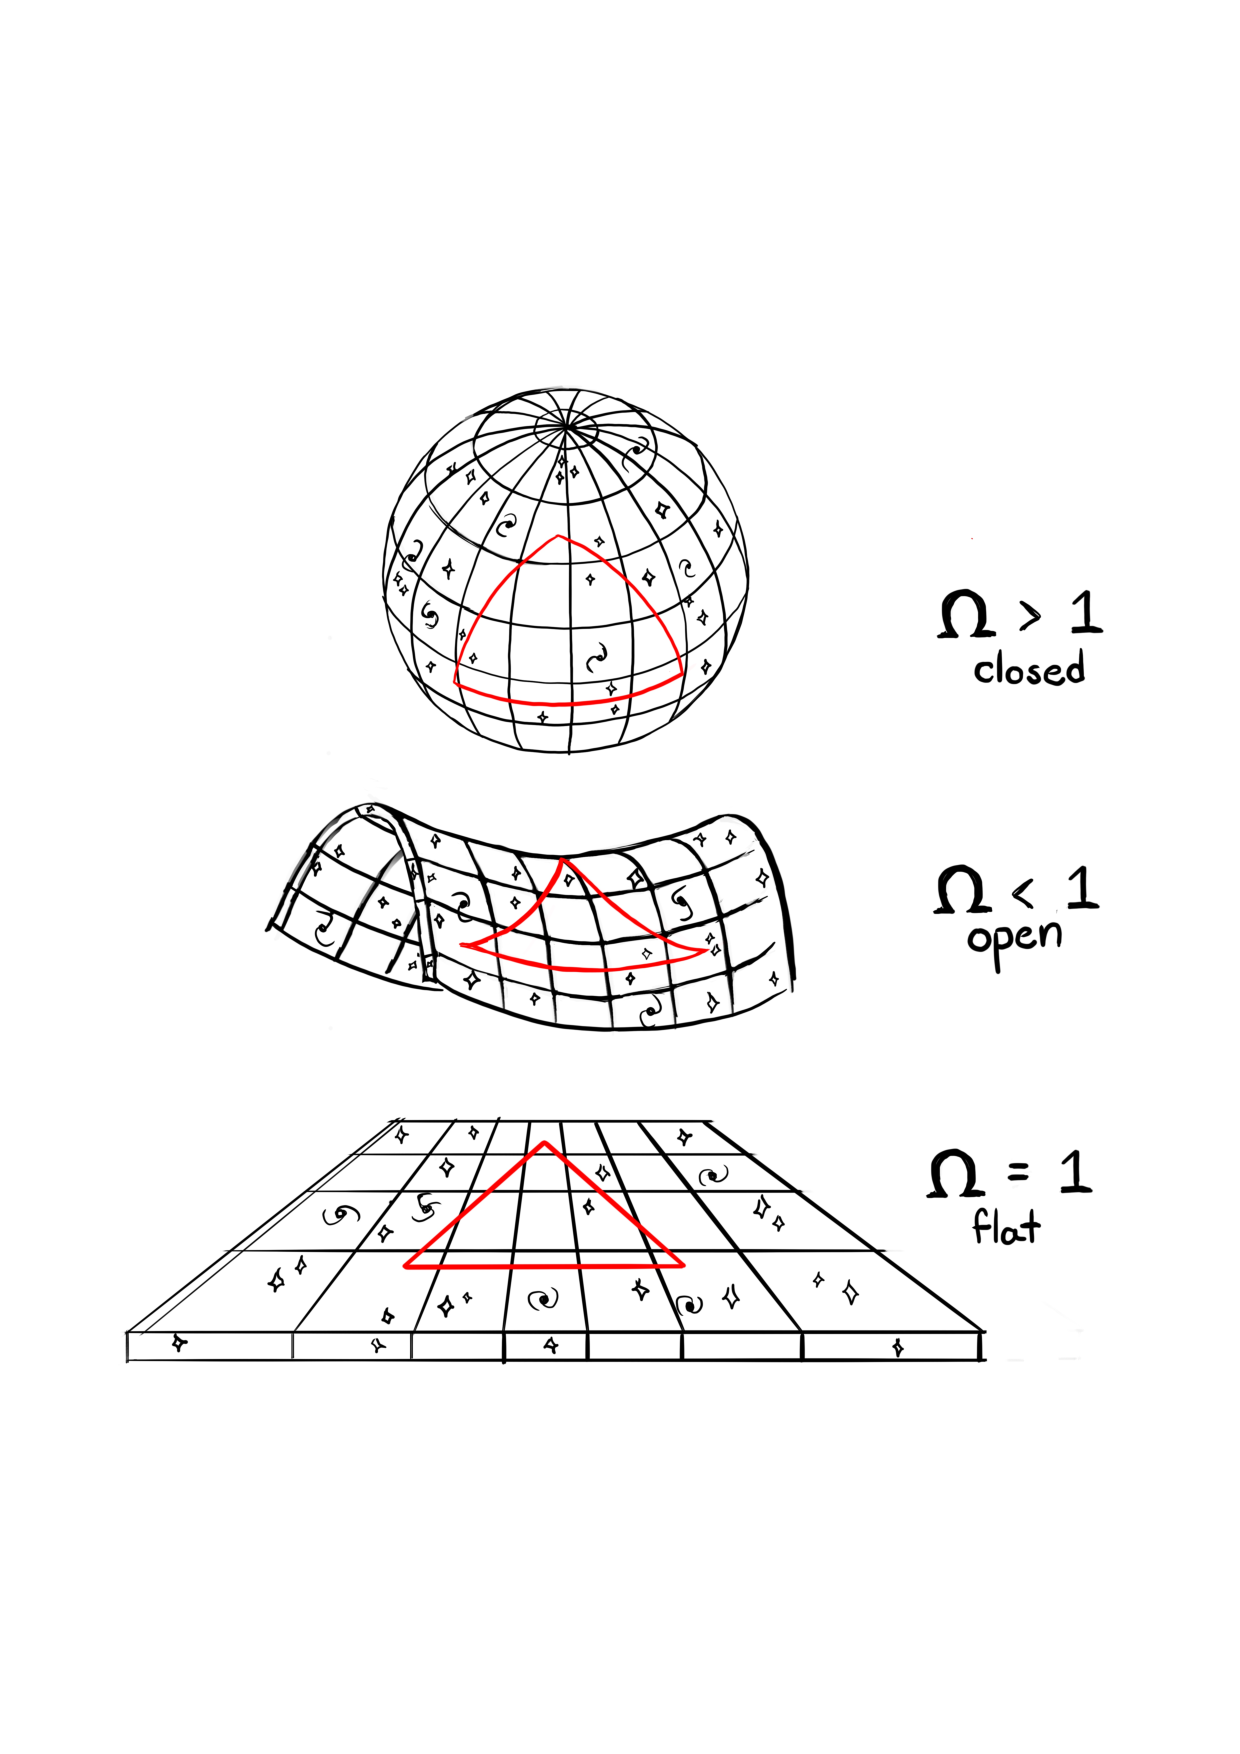
\includegraphics[width=\columnwidth]{Intro-FIGS/universeGeometry}
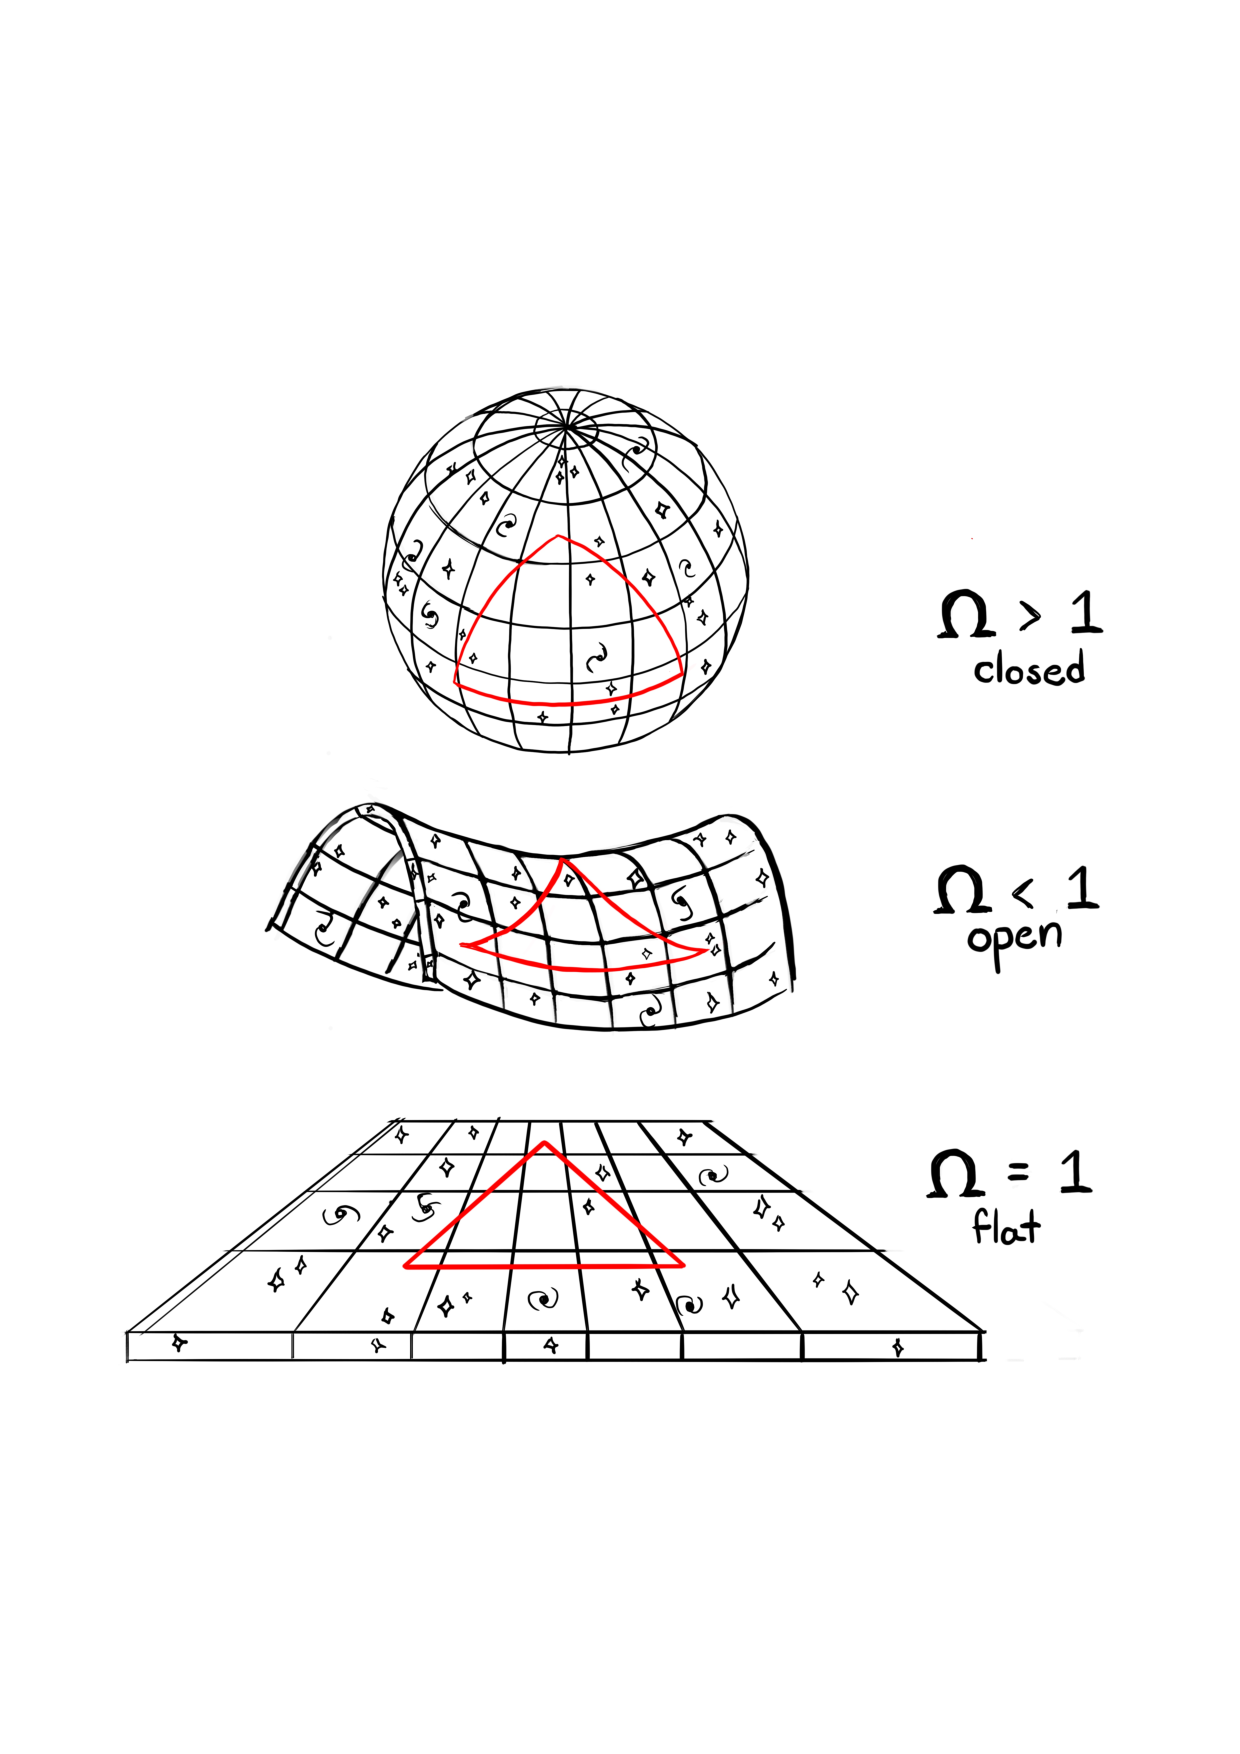
\includegraphics[width=\textwidth]{Intro-FIGS/universeGeometry}
\caption[Artistic representation of the geometry of the Universe and its matter-energy content. Figure created by R. Jackson.]{An artistic representation of the three geometries considered in the FRW metric -- Equation \eqref{Eq:Intro:FRW2} -- and their relationship between the total density of the Universe and the critical density, the dimensionless density parameter $\Omega \equiv \rho/\rho_c$. \textit{(top)} If $K = 1$ in Equation \eqref{Eq:Intro:Sk}, the total density is bigger than the critical density ($\Omega > 1$) and the geometry of the Universe is \textbf{closed}, meaning that the sum of internal angles of a 2D triangle is $> 180^o$. \textit{(middle)} If $K = -1$, total density of the Universe is smaller than the critical density ($\Omega < 1$) and the geometry of the Universe is \textbf{open} -- sum of internal angles of the 2D triangle is $< 180^o$. \textit{(bottom)} The last case happens when $K = 0$, when the total density of the Universe is precisely the critical density ($\Omega = 1$), this leads to a \textbf{flat} geometry for the Universe -- the usual Euclidean case, with the sum of internal angles of a triangle being precisely $180^o$. (Figure created by R. Jackson)}
\label{fig:Intro:Geometry}
\end{center}
\end{figure}

\subsubsection{Cosmological redshift}
Following the discovery made by \cite{1929Hubble}, nearby galaxies in the local Universe obey a linear law relating their distance and the rate at which they are distancing from a observer: $v = H_0x$. This relation is also known as \textbf{Hubble-Lema\^itre law}\footnote{Recently, during the 30th Meeting of the International Astronomical Union (IAU) in Vienna, the astronomical community decided to change this relation from `Hubble's law' to `Hubble-Lemaître law' \citep{2018IAU-HubbleLemaitre}.} -- where $H_0$ is referenced in modern cosmology as the \textbf{Hubble constant}. From the FRW metric, the physical distance between two fundamental observers (observers at rest in relation to the expansion of the Universe) is $R(t)dr$. Using this relation, Hubble's law can be re-written in a more generic fashion as 
\begin{equation}
H(t) = \frac{\dot{R}(t)}{R(t)}\, ,
\end{equation}
where the dot denotes a temporal derivative. 

\qquad At small scales, one can define the cosmological redshift in terms of the ration between the wavelength at the source of light and the observed light wavelengths,
\begin{equation}
\frac{\lambda_{\text{obs}}}{\lambda_{\text{source}}}  \equiv 1 + z\, ,
\end{equation}
where $z$ is the cosmological redshift as usually referenced in the literature. 

\qquad A general definition can be achieved when one considers a photon's null geodesic (in the absence of external forces or gravitational fields). As photons propagate radially in a geodesic, the FRW metric leads to 
\begin{equation}
r = \int \frac{dt}{R(t)}.
\end{equation}
Following, the comoving distance should be the same for all fundamental observers, therefore the integral above leads to
\begin{equation}
\frac{dt_{\text{source}}}{dt_{\text{obs}}} = \frac{R(t_{\text{source}})}{R(t_{\text{obs}})}.
\end{equation}
A conclusion here is that there is a time-dilation for photons emitted at distant galaxies which is proportional to the expansion of the Universe. This effect is reflected, as expected, in the observed wavelength yielding
\begin{equation}
\frac{1}{a(t)} = \frac{\lambda_{\text{obs}}}{\lambda_{\text{source}}}  \equiv 1 + z \, ,
\end{equation}
where $a(t) \equiv R(t)/R(t_0)$ is the dimensionless scale factor, i. e. the scale factor at a given time $t$ in terms of the current value of $R$ at the present time, $t_0$. In other words, $a(t_0) = 1$.

\qquad The ability to link the wavelength of light to the expansion of the Universe is a core concept in modern cosmology. As an example, it facilitates measurements of distance in the radial direction using spectra from spectroscopic surveys, or through the redshifted line-breaks of some types of galaxies through photometric bands' filters in photometric surveys \citep{AbdallaPhotoZ2011,2018-redshift}.

%%%%%%%%%%%%%%%%%%%%%%%%%%%%%%%%%%%%%%%%%%%%%%%%%%%%%%%%%%%
%					LCDM PARADIGM
%%%%%%%%%%%%%%%%%%%%%%%%%%%%%%%%%%%%%%%%%%%%%%%%%%%%%%%%%%%

\subsection{The $\Lambda$CDM Paradigm}\label{Sec:Intro:LCDM}
In the previous section, a relationship between geometry and the energy density content of the Universe appeared, relating $\Omega$ and $K$. In pursuance of a standard model for cosmology, the right hand side of Einstein's field equations, the energy-momentum tensor, needs to be defined. As this object must also obey the Cosmological Principle, it needs to be isotropic and homogeneous; a \textbf{perfect fluid} is a suitable candidate to describe the Universe in large scales. The energy-momentum tensor for a perfect fluid can be written as
\EQ{Intro:Tmunu1}{
T^{\mu\nu} = -(\rho + p)\frac{dx^{\mu}}{ds}\frac{dx^{\nu}}{ds} - g^{\mu\nu}p,
}
where $\rho$ is the energy density and $p$ is the pressure exerted by the fluid. The expression from Equation \eqref{Eq:Intro:Tmunu1} can be re-written in comoving coordinates as
\EQ{Intro:Tmunu2}{
T^{\mu}_{\ \ \nu} = \left( \begin{array}{cccc}
-\rho & 0 & 0 & 0 \\
0 & p & 0 & 0 \\
0 & 0 & p & 0 \\
0 & 0 & 0 & p\end{array} \right).
}

\qquad Inserting the energy-momentum tensor above with the FRW metric into Einstein's field equations, one finds the dynamical equations governing the behaviour of the scale factor. First, one obtains the non-trivial components of the Einstein tensor as

\EQ{Intro:EFE_LCDM}{
G_{00} & = \frac{3}{a^2}\left( \dot{a}^2 + K \right) \, , \\
G_{ij} & = \frac{1}{a^2}\left( 2a\ddot{a} + \dot{a}^2 + K \right)\delta_{ij},
}
where $\delta_{ij}$ is the Kronecker delta. Next, including the energy-momentum tensor from Equation \eqref{Eq:Intro:Tmunu2} \citep{1922Friedmann,1924FriedmannCurvature}:

\EQ{Intro:Fried1}{
\left(\frac{\dot{a}}{a}\right)^2 & = \frac{8\pi G}{3}\rho - \frac{K}{a^2} + \frac{\Lambda}{3}\, ,}
and

\EQ{Intro:Fried2}{
\frac{\ddot{a}}{a}&  = -\left\lbrace 4\pi Gp + \frac{1}{2}\left[\left(\frac{\dot{a}}{a}\right)^2 + \frac{K}{a^2}\right] \right\rbrace + \frac{\Lambda}{3}\, .
}

\qquad These are known as the Friendmann Equations \citep{1922Friedmann,1924FriedmannCurvature}, combining them leads to

\EQ{}{
\frac{\ddot{a}}{\dot{a}} = -\frac{4\pi G}{3}(\rho + 3p)\, ,
}
which implies that the acceleration is independent of the geometry, $K$. However, one can re-write Equation \eqref{Eq:Intro:Fried1} to obtain an expression for $K$ in terms of the time dependent variables $a(t)$, $\rho (t)$, and $p(t)$ \citep{padmanabhan_1999}. At the present time, $a(t=t_0) = 1$ \citep{1924FriedmannCurvature}, 

\EQ{Intro:K}{
K & = \frac{8\pi G}{3} \rho (t_0) - \dot{a}^2(t_0) + \frac{\Lambda}{3} \\
& \equiv  H_0^2(\Omega(t_0) - 1)\, ,
}
here, $H_0$ is the Hubble constant measured today and $\Omega \equiv \rho/\rho_c$ is again the dimensionless total density of the Universe. The critical density, $\rho_c$, is defined to be the precise energy density the Universe needs so its geometry is flat, i. e. $K=0$; it can be defined from Equation \eqref{Eq:Intro:K} as $\rho_c \equiv 3H_0^2/8\pi G = 8.098 \times 10^{-11} \text{eV}^{4}$. Figure \ref{fig:Intro:Geometry} shows the relationship between the total density of the Universe and its geometry.

\qquad It is useful to express Equation \eqref{Eq:Intro:Fried2} in terms of the Universe's components and their evolution according to the scale factor: pressureless matter (baryonic or dark), $\rho_m = (\rho_{b} + \rho_{cdm}) \propto a^{-3}(t)$; radiation, $\rho_r \propto a^{-4}(t)$; and vacuum energy, $\rho_{\Lambda} = \Lambda/8\pi G$. Using these relations, the second Friedmann equation -- Equation \eqref{Eq:Intro:Fried2} -- can be expressed in terms of the Hubble constant

\EQ{Intro:HubbleOmega1}{
E^2(t) \equiv \frac{H^2(t)}{H_0^2} = \left[ \Omega_r a^{-4}(t) + \Omega_m a^{-3}(t) + \Omega_K a^{-2}(t) +  \Omega_{\Lambda} \right], 
}
where the $\Omega_i$ are the dimensionless density of each component $i$ considered

\EQ{}{
\Omega_r \equiv \frac{\rho_r(t_0)}{\rho_c} \, ; \quad \Omega_m \equiv \frac{\rho_m(t_0)}{\rho_c} \, ; \quad \Omega_{\Lambda} \equiv \frac{\rho_{\Lambda}}{\rho_c} \, ; \\ 
\Omega_K \equiv 1 - (\Omega_r + \Omega_m + \Omega_{\Lambda}) = 1 - \Omega \, .
}
Promptly, Equation \eqref{Eq:Intro:HubbleOmega1} can be written in terms of the equation-of-state, $w_i$, for each of the components

\EQ{Intro:HubbleOmega2}{
E^2(t) & = \sum_i \Omega_i a^{-3(1+w_i)} \\
	& = \sum_i \Omega_i(1+z)^{3(1+w_i)}
}
with

\EQ{Intro:EoS}{
w_i = 
\begin{cases}
1/3, & \text{for radiation} \\
0, & \text{for matter (dark and baryonic)} \\
-1/3, & \text{for curvature}\\
-1, & \text{for vacuum or cosmological constant}
\end{cases}
}

\qquad Now, the comoving distance at a given redshift can simply be expressed as

\EQ{Intro:Comoving}{
\chi (z) = \frac{1}{H_0}\int_0^z \frac{dz'}{E(z')}
}
which means that distance measurements in comoving coordinates depend on the energy density content of the Universe at a given redshift. 

\qquad A brief description of each of the components of the Universe follows in the next subsections \citep{dods,schneider_2016}.

\subsubsection{Radiation, $\Omega_r$ :}
 Cosmic microwave background experiments such as COBE \citep{COBE}, WMAP \citep{WMAP_MapsResults,WMAP_Cosmology}, and the Planck Satellite \citep{2018PlanckCosmology} all measure the temperature of the CMB photons. The CMB photon temperature has been measured with incredible precision already with the FIRAS instrument (on-board of the COBE satellite) to be a perfect fit of a black-body radiation with $T_{cmb} = 2.725\pm 0.002$K \citep{1999FIRAS}. The energy density of photons can be estimated from statistical mechanics using the Bose-Einstein distribution function \citep[][p. 40]{dods}
 
 \EQ{Intro:CMB:Temp}{
 \rho_{\gamma} & = 2\int \frac{d^3p}{(2\pi)^3} p \left( e^{p/T_{cmb} -1 }\right)^{-1} \\
 	& = \frac{\pi^2}{15}T_{cmb}^4 \\
    & = \frac{\pi^2}{15}\left( \frac{2.725 K}{a} \right)^4
 }
and the equation-of-state for radiation is consistent with the pressure exerted by this component, $p_r = \frac{1}{3}\rho_r$. In terms of the dimensionless radiation density, $\Omega_r \approx 5 \times 10^{-5}$ \citep[][p. 182]{schneider_2016}.

\qquad Part of the radiation content is also composed of neutrinos, even thought the mass of these particles are small, it is known that it is non-zero \citep{Kamiokande1998}. Neutrinos, therefore, act relativistically at decoupling causing them to behave as radiation in the early Universe.

\begin{figure}
\begin{center}
%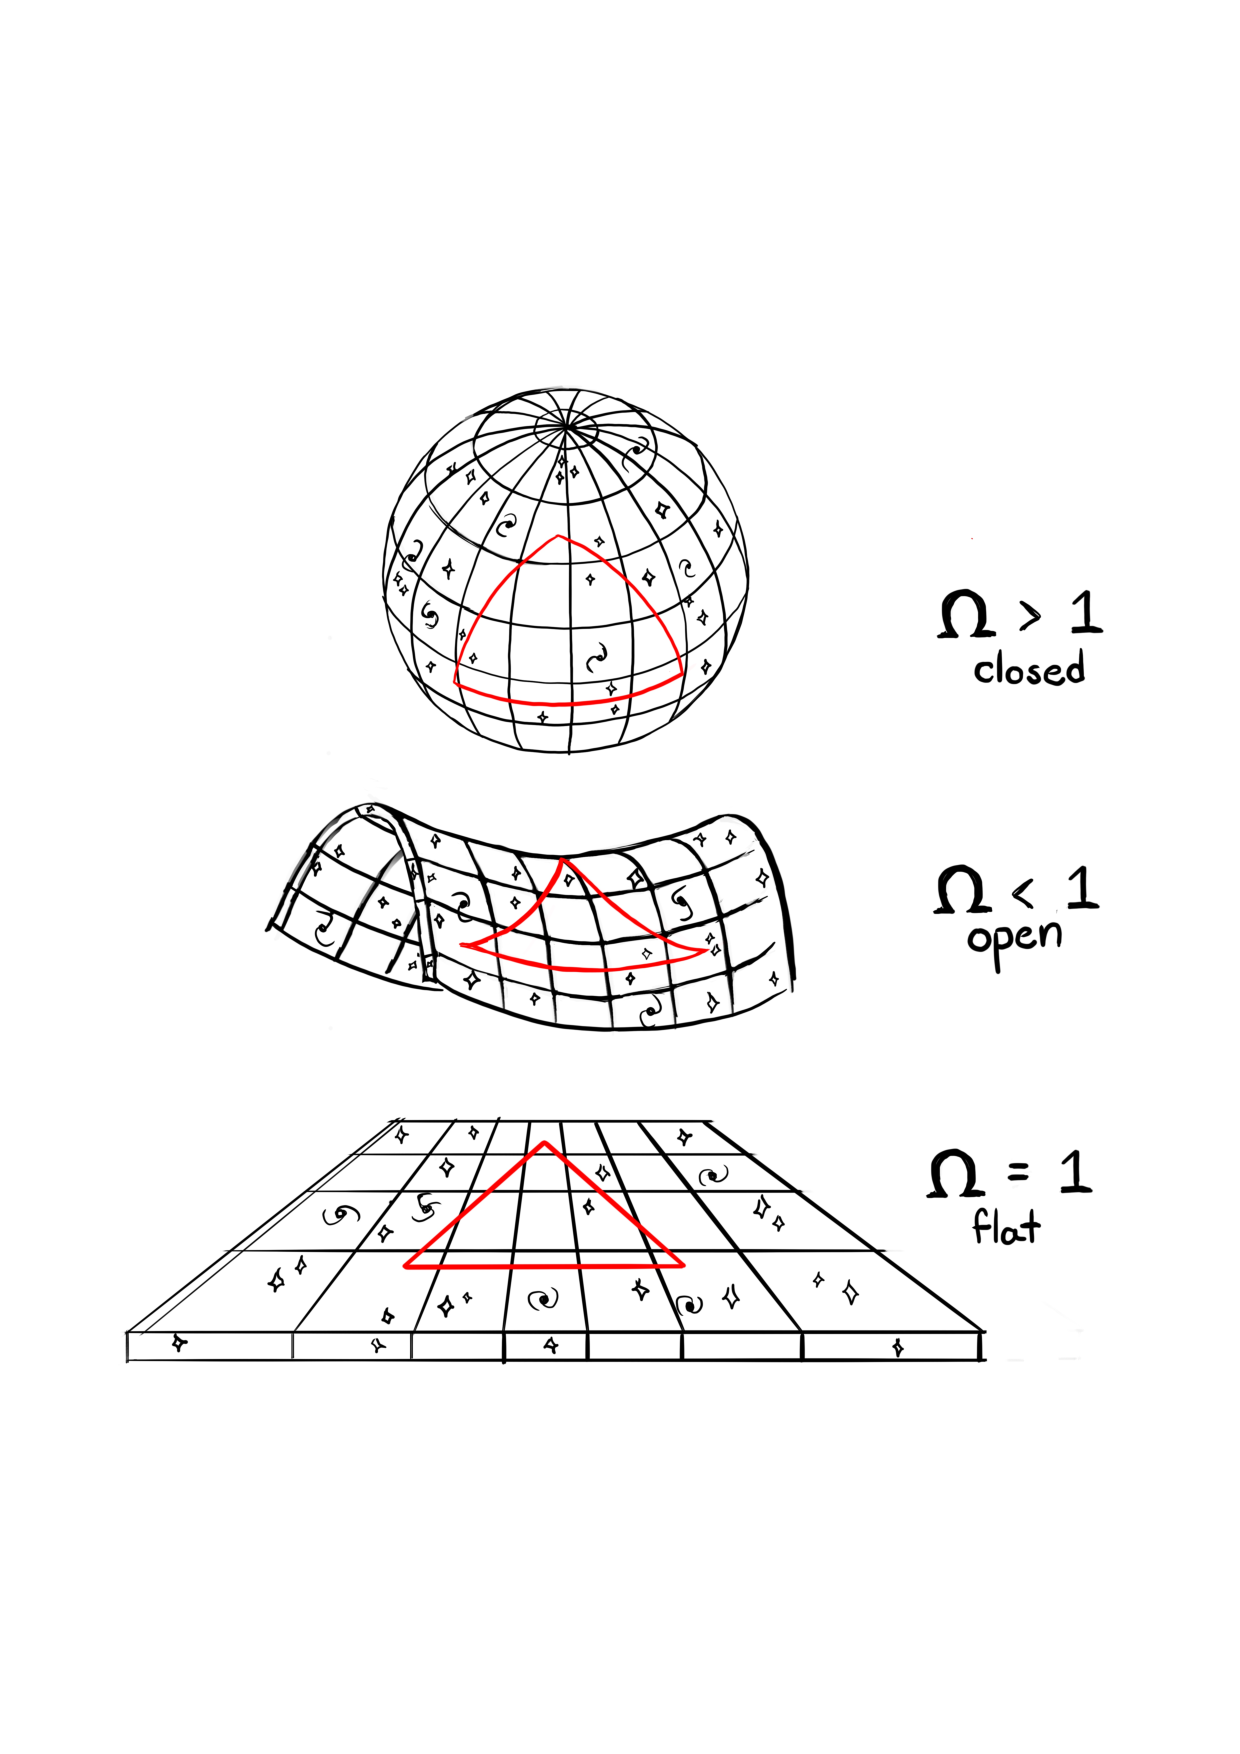
\includegraphics[width=\columnwidth]{Intro-FIGS/universeGeometry}
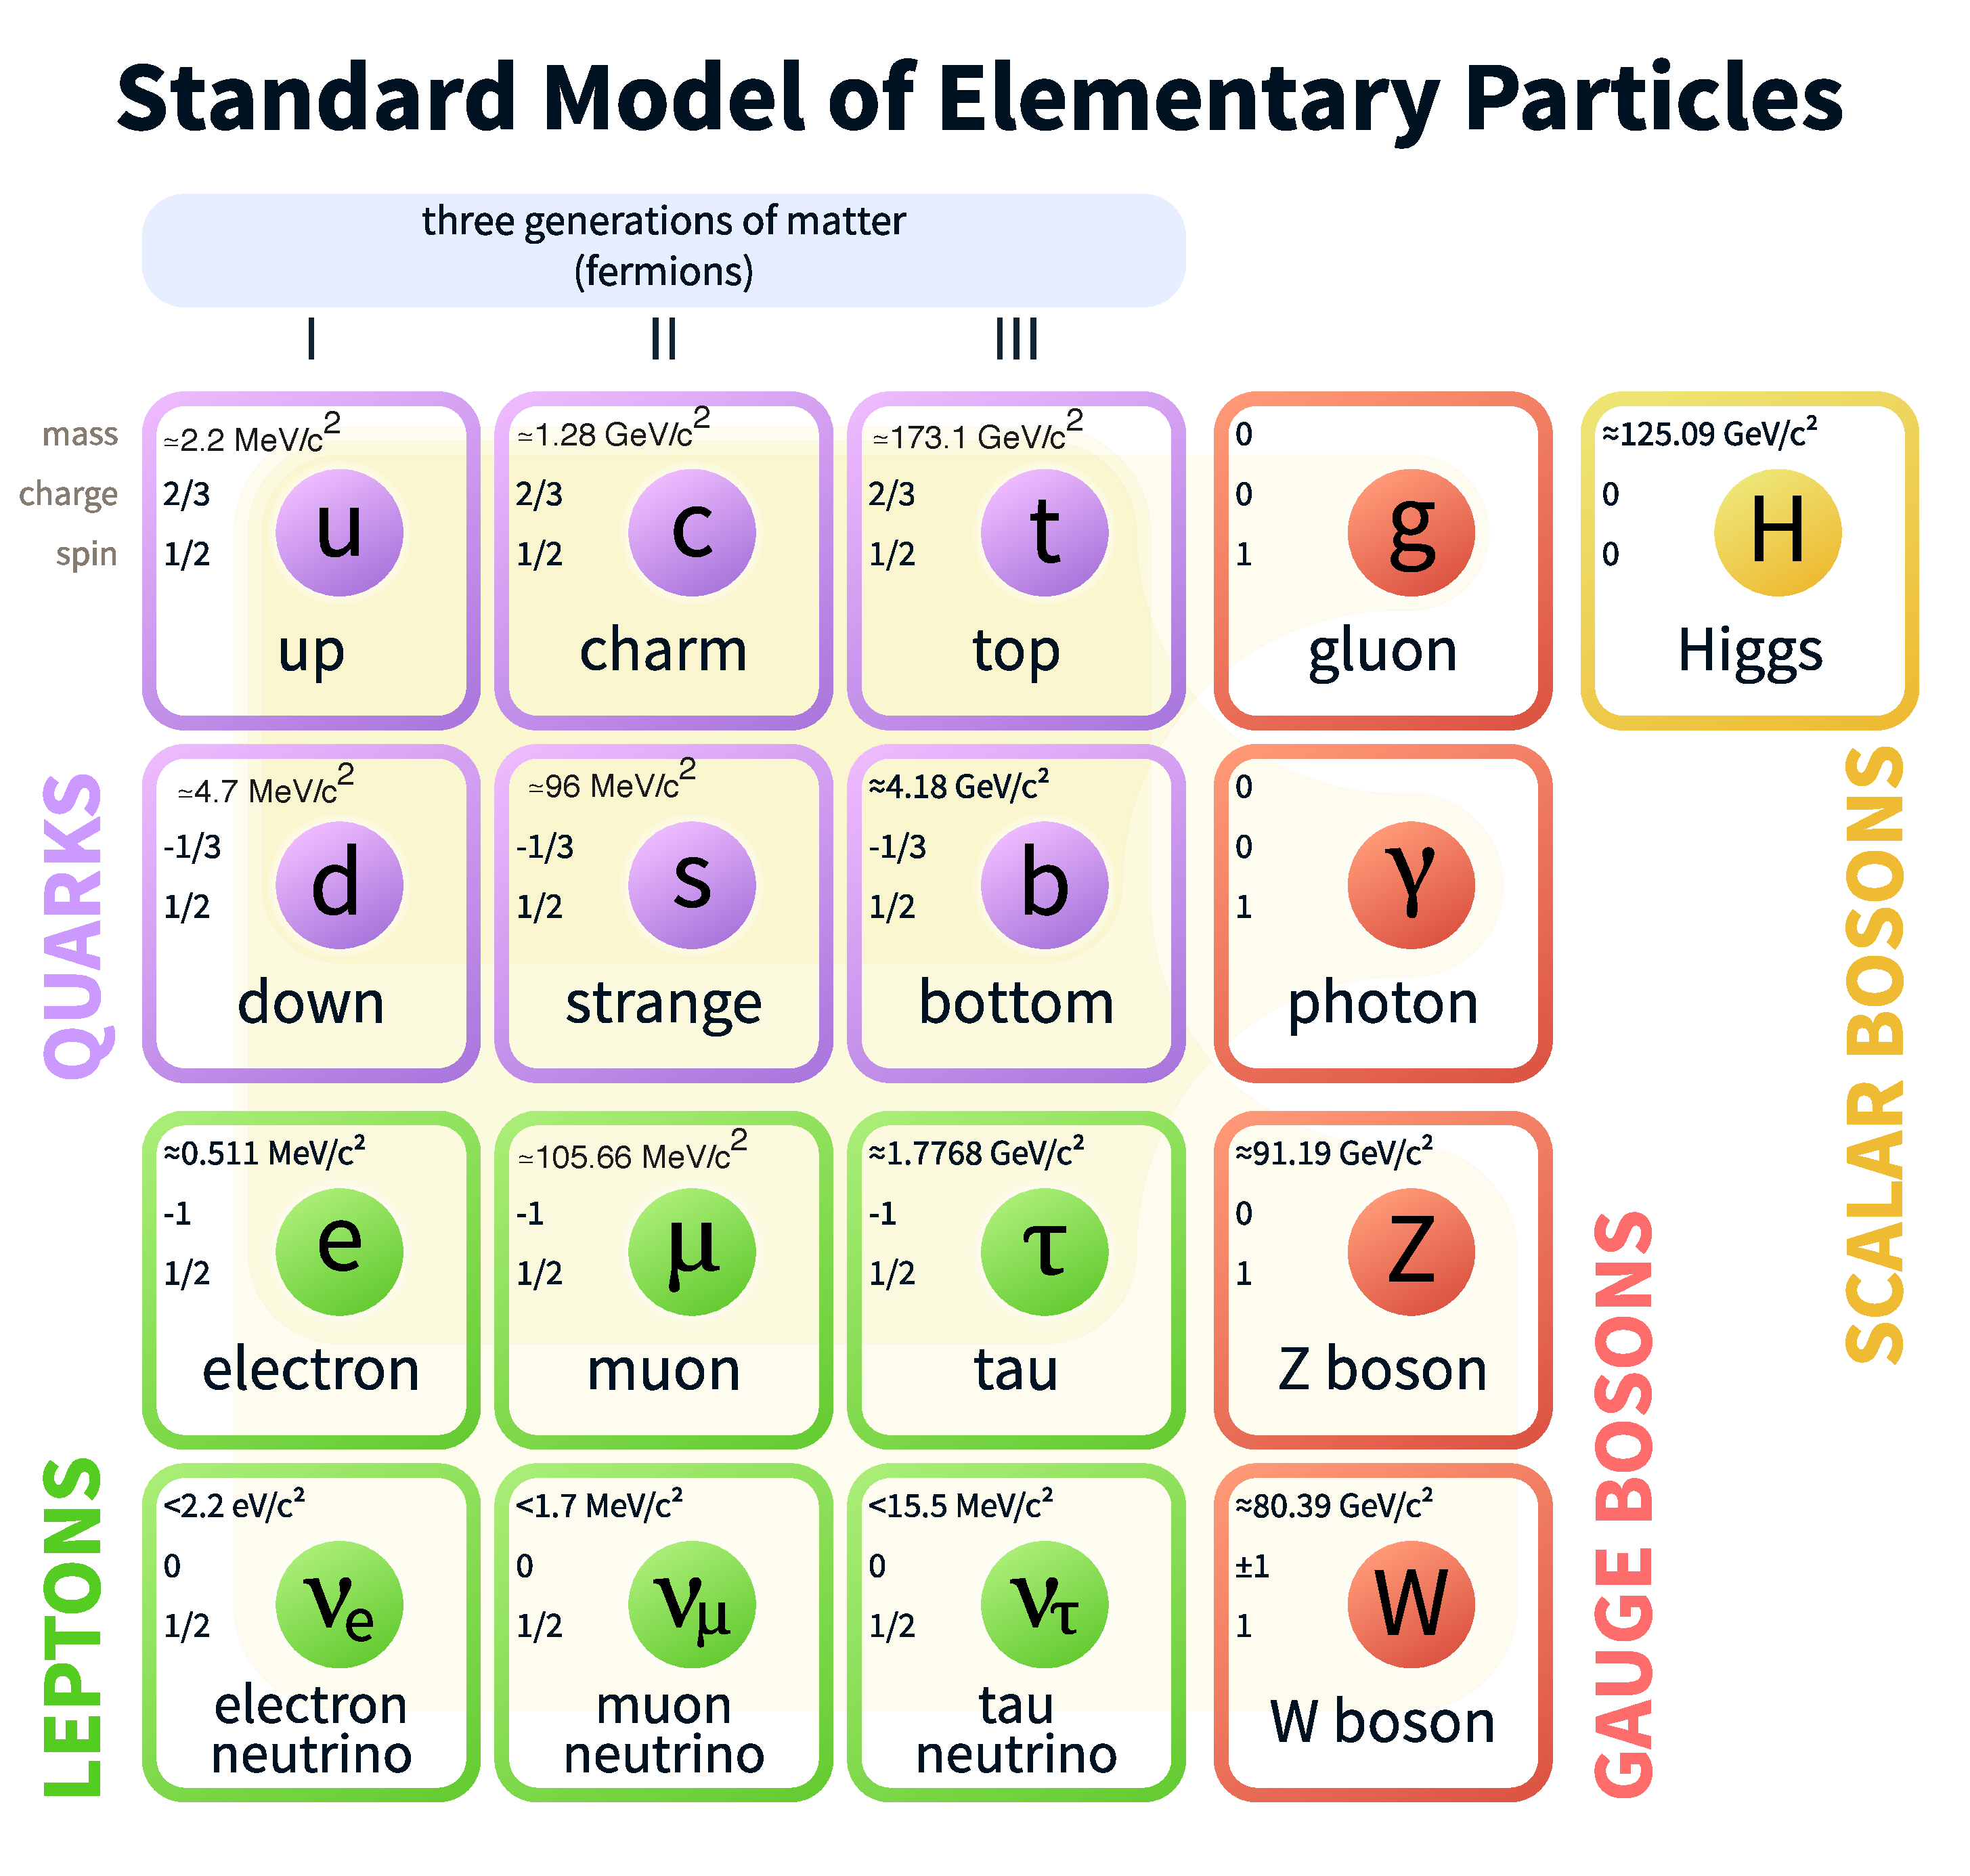
\includegraphics[scale=0.30]{Intro-FIGS/standard_model}
\caption[Standard Model of Particle Physics. (Source: Particle Data Group -- \url{http://pdg.lbl.gov})]{Standard Model of Particle Physics: \textit{(purple)} the six quarks; \textit{(red)} the four gauge bosons: gluon (strong force), photon (electromagnetic force), Z and W bosons (weak force); \textit{(green)} the six leptons: the three neutrino species and their charged counterparts; \textit{(yellow)} the newly experimentally discovered Higgs bosons, a scalar boson. All of these particles, with the exception of the W boson and the photon, have their associated anti-particle. The top values in the neutrino boxes show the upper bounds for each flavour's mass. (Source: Wikipedia, Particle Data Group -- \url{http://pdg.lbl.gov})}
\label{fig:Intro:StandardModel}
\end{center}
\end{figure}

%%%%%%%%%%%%%%%%%%%%%%%%%%%%%%%%%%%%%%%%%%%%%%%%%%%%%%%%%%%
%					ENERGY CONTENT
%%%%%%%%%%%%%%%%%%%%%%%%%%%%%%%%%%%%%%%%%%%%%%%%%%%%%%%%%%%

\subsubsection{Baryonic Matter, $\Omega_b$ :}
Baryonic matter constitutes all matter as we commonly refer to: all the atoms in the periodic table, electrons, neutrons, protons and more. In other words, any sort of particles described by the Standard Model of Particle Physics (Figure \ref{fig:Intro:StandardModel}) -- apart from neutrinos which, even though being massive, behave close to being relativistic in the early Universe. The baryonic matter density behaves similarly to a gas with a certain temperature but with zero chemical potential. Baryons interact with other components not only via gravitational interaction but also via the electromagnetic force. Therefore, baryons and photons are coupled throughout the history of the Universe; during this phases, baryonic matter has an equation-of-state $p = \rho/3$. After photons and baryons decouple, this component behaves as a pressureless fluid with an equation-of-state $p=0$. 

\qquad In a seminal work by \cite{1998BaryonContent}, the authors estimate the baryonic content of the Universe using four different methods at low redshift ($z \approx 0$), high redshift ($z\approx 3$) gas components, and big bang nucleosynthesis (BBN) abundances \citep{2000-BBN-Review,2016R-BBN-Review}. The low redshift indicators contain stars in elliptical, spiral, and irregular galaxies, neutral atomic gas, plasma in clusters, warm and cool plasma in the intermediate mean in cluster groups -- with a sum of $\Omega_b = 0.021$. High redshift indicators constitute damped absorbers and Ly$\alpha$ forest clouds \citep{2003Weinberg-Lyalpha}, representing a value of $\Omega_b$ agreeing with the low redshift measurements. From BBN, the abundances of Deuterium and Helium also indicate a baryonic content of $\Omega_b \approx 0.021\pm 0.007$. These values are consistent with the current value found by \cite{2018PlanckCosmology} ($\Omega_b h^2 = 0.0224 \pm 0.0001$) and the values found in BOSS analysis in Chapter \ref{Chap:BOSS-Cosmo}.

\subsubsection{Cold Dark Matter, $\Omega_{cdm}$:}
Cold dark matter is inferred indirectly via several observations -- including the rotational curves of galaxies \citep{1970Rubin,1973RobersRots} and gravitational lensing measurements in galaxy clusters \citep{2006BulletCluster} -- indicating that the majority of matter in the Universe is electromagnetically non-interactive, non-relativistic, and non-luminous. This strange component interacts only gravitationally and, as a consequence, it is not coupled to photons. This causes dark matter to start clustering earlier than baryonic matter. As there is no coupling, this component also behaves as a pressure-less fluid, $p_{cdm} = 0$, since very early in the Universe. The correlation function of galaxies \citep{Einsenstein2005}, the power spectra of galaxies \citep{Blake2007,BOSS}, and the CMB acoustic peaks \citep{PlanckCosmology2016,PlanckResults2015,2018PlanckCosmology} also need the additional existence of cold dark matter in order to explain the baryon acoustic oscillation (BAO) peak and other features of the 2-point statistics in the analysis (see Section \ref{Sec:Intro:Pk}). These measurements combined seem to suggest that $\Omega_{cdm} \approx 0.25$ .

\qquad Empirical evidence for cold dark matter comes only through indirect gravitational observations, no direct detection were made so far \citep{2017DarkMatterExpReview}. In light of these null detection, there are some attempts to explain it with alternative theories. In the early years, neutrinos were a good candidate for dark matter as they interact very weakly via the electromagnetic field. Although, this hypothesis was later discarded as they later proved to behave more as a hot dark matter -- washing away structure instead of forming it earlier as CDM. Some other alternative theories came from questioning the nature of GR, like Modified Newtonian Dynamics (MOND, \citealt{1983MOND}). MOND tries to explain the observational effects attributed to cold dark matter by introducing an acceleration scale in which Newtonian dynamics is modified. Even though it was created in order to solve the observations explained by dark matter, there are several issues with this theory where it fails to explain other dark matter observations \citep{2011MondSucks}. One of them, claimed as `a direct empirical proof of the existence of dark matter' by \cite{2006BulletCluster} can only be explained by MOND if the sum of mass of neutrinos were $\sum m_{\nu} \approx 2.0$ eV \citep{2007ApJ...654L..13A}. Such value is already excluded by galaxy clustering measurements -- \citealt{Thomas2010Neutr,2014Gonzalez-GarciaNeutrino} as well as measurements shown in Chapters \ref{Chap:BOSS-Cosmo} and \ref{Chap:Neutrinos} -- which makes MOND very unlikely to be true.  

\subsubsection{Cosmological Constant or Dark Energy, $\Omega_{\Lambda}$ or $\Omega_{de}$:}
Observations of Supernovae type Ia luminosity distance--redshift relation strongly suggest that something is causing the Universe to go through an accelerated expansion phase \citep{1998Riess,1999Perlmutter,2018LambdaCentury}. The furthest away galaxies are, the faster they distance themselves from each other. This effect is attributed to a mysterious component called dark energy which seems to compose around $70\%$ of the Universe \citep{2018PlanckCosmology}. This component seems to exert a negative pressure, $p_{de} \leq - \rho_{de}$; it can be parametrised in terms of the equation-of-state parameter, $w_0$ -- where, if $w_0 = -1$, dark energy is simply the cosmological constant, $\Lambda$, as $p_{\Lambda}= - \rho_{\Lambda}$. Any deviation from $w_0 = -1$ would mean new physics, beyond the standard $\Lambda$CDM model. Current observations from the Dark Energy Survey combined with BAO measurements from BOSS \citep{2016BOSSCosmology}, and CMB from Planck \citep{PlanckCosmology2016} seem to suggest that $w_0 = -1.00^{+0.04}_{-0.05}$. Measurements shown in Chapter \ref{Chap:BOSS-Cosmo} are consistent with the DES findings; these seem to suggest that dark energy is simply the cosmological constant, $\Lambda$. A lot of questions are still unanswered in Cosmology as the nature of $\Lambda$ is still unknown -- if one does not accept it as a fundamental property of spacetime.

\qquad As an extension of the standard dark energy model, via parametrising $w_0$, it is common to generalise Equation \eqref{Eq:Intro:HubbleOmega2} for a case where the equation-of-state of dark energy varies over redshift \citep{2001Chevallier,2011Shi,2014DarkEnergyReview}. For a flat Universe, 

\begin{equation}
    E^2(z) = \left[ \Omega_r (1+z)^4 + \Omega_m(1+z)^3 + (1 - (\Omega_r+\Omega_m))f(z)\right],
\end{equation}
where $\Omega_{de} \equiv 1 - (\Omega_r+\Omega_m)$ is the normalised energy density of dark energy. The redshift evolution for this quantity is now encompassed into the function, $f(z)$, and it can be generically expressed by \citep{2011Shi,2014DarkEnergyReview}: 

\begin{equation}
    f(z) \equiv \frac{\rho_{de}(z)}{\rho_{de}(z=0)} = \exp \left\{ 3 \int_0^z [1 + w(z')]\frac{dz'}{(1+z')} \right\}.
\end{equation}
For the case where there's no redshift dependency on the equation-of-state of dark energy, the same expression as in Equation \eqref{Eq:Intro:EoS} is recovered, i. e. $\rho_{de}(z)/\rho_{de}(z=0) = (1+z)^{3(1+w_0)}$. However, current state-of-the-art cosmological data does not contain sufficient constraining power to determine if such redshift evolution on $w(z)$ exists or not \citep{ 2016BOSSCosmology,2018PlanckCosmology}.


\subsubsection{Neutrinos, $\Omega_{\nu}$:}
Produced by weak force interactions, neutrinos come in three different leptonic flavours: neutrino electron ($\nu_e$), neutrino muon ($\nu_{\mu}$), and neutrino tau ($\nu_{\tau}$); which are all associated with their corresponding charged leptons: electron, muon, and tau (see Figure \ref{fig:Intro:StandardModel}). As mentioned, experiments in the late 90s like the Super Kamiokande \citep{Kamiokande1998} and subsequent experiments \citep{2002SNO,2005KamLAND,2008MINOS,2012RENOExperiment,AbeNeutrino2014} demonstrated that neutrinos oscillate between flavours which was a smoking gun to the theory that neutrinos have finite mass eigenstates. The total mass of neutrinos and their hierarchy (or ordering) is still unknown as particle physics oscillation experiments can only measure the square mass splitting between species \citep{2014Gonzalez-GarciaNeutrino}:

\begin{align}
\Delta m_{21}^2 & \equiv m_2^2 - m_1^2 \nonumber \\ 
				& \approx 7.49^{+0.19}_{-0.17} \times 10^{-5}\, \text{eV}^2 \label{Eq:Intro:Mass21}
\end{align}
\begin{align}
|\Delta m_{31}|^2 & \equiv |m^2_3 - m_1^2| \nonumber \\ 
				  & \approx 2.484^{+0.045}_{-0.048} \times 10^{-3} \, \text{eV}^2. \label{Eq:Intro:Mass31}
\end{align}
The measurement in Equation \eqref{Eq:Intro:Mass21} comes from solar neutrino oscillation experiments, while the measurement in Equation \eqref{Eq:Intro:Mass31} comes from atmospheric neutrino oscillation experiments. Both these measurements imply that at least two of the neutrino species have a non-zero mass. However, as the signal in the $|\Delta m_{31}|^2$ is unknown, two different hierarchies are possible if the masses are not completely degenerate.

\qquad The large scale structure of the Universe is sensitive to the sum of neutrino mass species, $\sum m_{\nu} = m_1 + m_2 + m_3$, as the cosmic neutrino density can be probed via the dimensionless density of neutrinos, $\Omega_{\nu} \propto \sum m_{\nu}$. In the early Universe, when the neutrino temperature was sufficiently high, the energy density of neutrinos is related to that of photons (Equation \ref{Eq:Intro:CMB:Temp}) as %$\Omega_{\nu} \approx \sum m_{\nu}/(93.14h^2 \, eV)$ \citep{dods}. 

\EQ{Intro:NuRho1}{
\rho_{\nu} = \frac{7}{8}\left( \frac{4}{11}\right)^{3/4}\rho_{\gamma}
}
where the factors in the above equation are related to the degeneracy factor of neutrinos, the fact that neutrinos are fermions and obey a Fermi-Dirac distribution which leads to a factor of $(4/11)^{1/3}$, and, finally, the energy density of massless particles scaling with temperature with $T^{4}$ for photons \citep[][p. 45]{dods}. For massive neutrinos, Equation \eqref{Eq:Intro:NuRho1} can be expressed as 
\EQ{}{
\rho_{\nu'} = \frac{2}{(2\pi)^3}\int d^3p \frac{\sqrt[]{p^2 + (m_{\nu'})^2}}{e^{p/T_{\nu'}}+1}.
}
for each individual neutrino species, $\nu'$. After the neutrino temperature ($T_{\nu'}$) drops to $T_{\nu'} \sim  m_{\nu'}$, massive neutrinos start behaving non-relativistically. For a specific massive species with mass $m_{\nu}$, this effect happens around a redshift of

\begin{equation}
    z_{\text{n-r}} \approx \frac{m_{\nu}}{3k_B T_{\nu,0}} \approx 2\times 10^3 \left(\frac{m_{\nu}}{1 \text{ eV}} \right),
\end{equation}
where $T_{\nu,0}$ is the present-day redshifted neutrino temperature \citep{2000-NeutrinosDarkMatter}, given by

\begin{equation}
    T_{\nu,0} = \left( \frac{4}{11}\right)^{1/3}T_{\gamma,0} = 1.947 \text{K},
\end{equation}
leading to an overall contribution to the energy density content of the Universe from neutrinos to be expressed as \citep{2003HannestadNeutrino}

\EQ{}{
\Omega_{\nu} \approx \frac{\sum m_{\nu}}{92.5h^2 \text{eV}}.
}

\qquad The redshift $z_{\text{n-r}}$ marks the moment at which neutrinos stop behaving as radiation and start behaving as matter. At this moment, the average neutrino background momentum is given by $\langle p_{\nu}\rangle = 3.15k_BT_{\nu}$; while after they become non-relativistic, the average speed is decribed as $\langle v_{\nu}\rangle \approx 160 \text{ km/h} \left( \frac{1 \text{eV}}{m_{\nu}}\right) \left( \frac{T_{\nu}}{1.947K}\right)$. Since the neutrino background temperature drops with $T_{\nu}\propto a^{-1}$, the massive neutrinos will slow down as the Universe expands \citep{2000-NeutrinosDarkMatter}. Since $z_{\text{n-r}}$ happens much later than the matter-radiation equality, $z_{eq}\sim 24000\Omega h^2$, neutrinos are still relativistic at this moment which prevents massive neutrinos from gravitationally clustering during this period. As a result, neutrinos `free-stream' introducing a characteristic length scale related to the horizon size at this epoch, $L_{fs} \approx 112 \text{ Mpc}\left( m_{\nu}/1 \text{ eV}\right)$ \citep{2000-NeutrinosDarkMatter,2003HannestadNeutrino,2017Lancaster-NeutrinosFreeStream}.

\qquad Still, massive neutrinos act as some sort of `warm dark matter' as they are almost relativistic while barely interacting with matter other than gravitationally -- this means that massive neutrinos tend to `wash away' structure in smaller scales. In \cite{2003HannestadNeutrino}, and more recently in \cite{2016Hannestad}, the authors demonstrate the case for measuring not only the upper limit for $\sum m_{\nu}$, but also the neutrino mass hierarchy from cosmological galaxy surveys. In Chapter \ref{Chap:Neutrinos}, I explore the impact of modelling the neutrino mass and neutrino mass hierarchy using different assumptions and datasets.


\subsubsection{Curvature, $\Omega_K$:}
As shown in Equation \eqref{Eq:Intro:K} and Figure \ref{fig:Intro:Geometry}, there is a direct relationship between the curvature of the Universe, its energy content, and the critical density, $\rho_c$. If $\Omega = 1$, the Universe is perfectly flat with $K=0$. Balloon-based experiments in the late 90s and early 00s, like BOOMERanG \citep{2000-BOOMERANG} and MAXIMA \citep{2000Hanany-MAXIMA}, were able to determine the overall geometry of the Universe by locating the first acoustic peak in the angular power spectrum of cosmic microwave background temperature anisotropies. \cite{2000-BOOMERANG} found a peak at a multipole $\ell_{\text{peak}} = 197\pm 6$ with an amplitude of $\Delta T_{\ell=200} = (69\pm 4) \pm 7$ mK\footnote{ These are 1-$\sigma$ statistical and calibration errors, respectively -- according to \cite{2000-BOOMERANG}}. The value of $\ell_{\text{peak}}$ is mostly sensitive to two main cosmological parameters: the angular diameter distance from the observer to decouple; and the acoustic sound horizon scale -- this is due to density fluctuations with scales near the size of the sound horizon at decoupling producing this first peak in the CMB power spectrum. A flat Universe would present a $\ell_{\text{peak}}\approx 200/\Omega^{1/2}$; meanwhile, an open (closed) Universe would shift the position of the first acoustic peak to higher (lower) multipoles.

\qquad Recent results from the Planck collaboration observations estimate $\Omega_K = 1 - \Omega = 0.0007\pm 0.0037$ \citep{2018PlanckCosmology}. This is a very strong observational evidence that the Universe is flat, meaning that the energy density of the Universe is precisely the critical density with 0.2\% accuracy. 

\vspace{5mm}

\qquad In summary, the $\Lambda$CDM background Universe can simply be described by a FRW metric, a perfect fluid, and the cosmological constant. The standard cosmological model implies that our Universe is going through an accelerated expansion phase in the present time, i. e. it is currently dominated by the cosmological constant, and contains a flat geometry. Distances are measured related to the scale factor, $a(t)$, which, according to the FRW metric evolves with time. Finally, the baryonic content of the Universe is insufficient to describe several cosmological and astrophysical observations, leading to the necessity of dark matter to explain these phenomena. 

\qquad There are still several pieces missing in the $\Lambda$CDM paradigm puzzle, the main ones being \textbf{the horizon problem} and the \textbf{flatness problem} \citep{1994Hu-Flatness-Horizon,2005Lake-PRL-Flatness,2012Helbig-flatness}. The first one, the horizon problem, is related to the thermalisation of photons in the CMB. Since signals can't travel faster than the speed of light, CMB photons separated by more than one degree in the sky should have originated from completely uncorrelated parts of the very early Universe. These means that no information, like temperature, between such regions could have been exchanged. This, however, is not what is observed in the cosmic microwave background. Fluctuations in the CMB temperature are of the order of $\Delta T/T \sim 10^{-5}$. The second issue, the flatness problem (also known as the coincidence problem), is related to the extreme coincidence that our Universe has precisely the energy density needed for it to be flat, i. e. $\Omega = 1$. For this to happen, a very careful ``fine-tuning'' in the early Universe's parameters was necessary. Although theories like \textbf{inflation} claim to solve both these issues (see \citealt{2008InflationReview} for a review), no cosmological observations seem to confirm even the simplest of predictions from inflation \citep{2014Bicep2Planck}.

\vspace{10mm}
%%%%%%%%%%%%%%%%%%%%%%%%%%%%%%%%%%%%%%%%%%%%%%%%%%%%%%%%%%%
%				INHOMOGENEOUS UNIVERSE
%%%%%%%%%%%%%%%%%%%%%%%%%%%%%%%%%%%%%%%%%%%%%%%%%%%%%%%%%%%
\section{Probing inhomogeneities in the Universe}
During the last section, I described the Universe at extremely large scales -- the background Universe. However, when observed in `not so large scales', structures like groups of galaxies, clusters, filaments, voids, and more appear. This demonstrates that at certain scales the Universe's behaviour is dominated by these inhomogeneities. The accelerated expansion of the Universe, combined with the attractive nature of gravity creates structures like groups and clusters of galaxies which are not randomly distributed in the sky. Rather, positions in the sky of such objects are correlated in a way that depends on the matter-energy density, geometry, and content of the Universe. This section will explore how to understand the Universe using the statistical distribution of galaxies and other probes of inhomogeneity.

\qquad Since the first galaxy redshift surveys, structures like the Great Wall \citep{SloanGreatWall} and the Great Attractor \citep{ScharfLahav1992} appeared in the distribution of galaxies indicating that much can be understood about the Universe by probing these inhomogeneities. When combining this observations with the CMB temperature anisotropies ($\Delta T/T \sim 10^{-5}$), it becomes clear that anisotropies in the CMB where the seed to the formation of structures in the late Universe. 

%%%%%%%%%%%%%%%%%%%%%%%%%%%%%%%%%%%%%%%%%%%%%%%%%%%%%%%%%%%
%				INHOMOGENEOUS UNIVERSE
%%%%%%%%%%%%%%%%%%%%%%%%%%%%%%%%%%%%%%%%%%%%%%%%%%%%%%%%%%%
\subsection{Linear perturbation Theory}\label{Sec:Intro:LinTheory}
Any attempt to describe the distribution of matter in the Universe in a deterministic way, trying to model the precise location of each celestial object, would lead to frustration and failure. Instead, one should attempt to describe the statistical properties of the distribution of matter in the Universe, i. e. to statistically describe the matter density field. When probing the way matter behaves in the presence of gravity in an expanding Universe, the \textbf{matter overdensity field} is an important tool;  it can be defined as
\EQ{Intro:OverdContrast}{
\delta(\textbf{r},t) \equiv \frac{\rho(\textbf{r},t) - \bar{\rho}(t)}{\bar{\rho}(t)},
}
where $\bar{\rho}(t)$ is the mean matter density in a given time or redshift. Over time, density fluctuations grow due to the gravitational interaction with nearby matter: over-dense regions will become denser with time, increasing the overdensity field locally; while under-dense regions will become less dense. In other terms, the module of the matter overdensity field, $| \delta |$ increases as the Universe evolves.

\subsubsection{Perturbations on Boltzmann equations:}
To obtain the evolution of the matter overdensity field, one needs to solve a series of coupled differential equations taking into account the coupling and evolution of all components described in Section \ref{Sec:Intro:LCDM}. Linear perturbation theory is a widely spread method to solve problems of this nature in physics. Here, I will follow a similar path and description as the one presented in \cite{Peacock} and \cite{dods} in which one solves the Boltzmann equations for each of the components of the Universe using perturbation theory in a FRW background Universe. 

\qquad Starting with the collisional Boltzmann equation and the occupation function for each component, \textit{f}, 
\EQ{Intro:Boltzmann}{
\frac{df}{dt} = \frac{\partial f}{\partial t} + \frac{dx^i}{dt}\frac{\partial f}{\partial x^i} + \frac{d p}{dt}\frac{\partial f}{\partial p} = \mathcal{C}[f]
}
where $\mathcal{C}[f]$ accounts for any sort of collisions and coupling a component might experience throughout the evolution of the Universe.

\qquad The left hand side of Equation \eqref{Eq:Intro:Boltzmann} takes into account perturbations in the background FRW metric. In a generic way, scalar perturbations in the metric can be described using four functionals: $A$, $B$, $C$, and $D$ \citep[][ p. 132]{dods}:
\begin{align}
    g_{00} & = -(1+2A)\, , \\
    g_{0i} & = -aB_{,i}\, , \\
    g_{ij} & = a^2\left( \delta_{ij} \left[ 1-2C \right] -2D_{,ij} \right)\, .
\end{align}

All four functionals are scalars and depend on both space and time variables. The conformal Newtonian gauge \citep[][p. 87]{dods} describes the background metric using two potentials with dependence on spacetime. In terms of the before-mentioned functionals: $A = \Psi (\textbf{r}, t)$, $C = -\Phi (\textbf{r}, t)$, and $B=D=0$\footnote{Here, I am following the convention set by \cite{dods}. In comparison to \cite{1980Bardeen} gauge invariant variables one has $\Phi_A = \Psi$ and $\Phi_H = -\Phi$. } \citep{1995Gauges}. In other words, the non-vanishing terms in the perturbed metric are
\EQ{Intro:PertMetric_00}{
g_{00}(\textbf{r},t)=-(1+2\Psi(\textbf{r},t))
}
and 
\EQ{Intro:PertMetri_ij}{
g_{ij}(\textbf{r}, t) = a^2(t)(1+2\Phi(\textbf{r},t))\delta_{ij}
}
which, for a Universe with no anisotropic stress, leads to $\Psi (\textbf{r},t) = - \Phi(\textbf{r},t)$ \citep{Peacock}. Equation \eqref{Eq:Intro:Boltzmann} can now be re-written as
\EQ{Intro:BoltzmannFinal}{
\frac{\partial f}{\partial t} +\frac{p\hat{p}_i}{a(t)E} \frac{\partial f}{\partial x^i}-\frac{\partial f}{\partial E}\left( \frac{p^2}{E}\dot{\Phi} + \frac{\partial \Psi}{\partial x^i}\frac{p\hat{p}_i}{a(t)} + \frac{p^2}{E}H(t)\right) = \left[ \frac{\partial f}{\partial t} \right]_{\mathcal{C}}\, ,
}
where E is the energy and p is the momentum with a unity directional vector $\hat{p}_i$ of a certain component of the Universe. This equation, together with the perturbed Einstein's field equations, describe fully the perturbation's evolution throughout the history of the Universe.

\qquad The Universe's components can be divided into two main categories: relativistic components -- like photons and neutrinos -- and non-relativistic components -- like dark and baryonic matter. Within the same category, components behave in a similar fashion; however, with different couplings. In Fourier space, the evolution of these components depends mainly on the magnitude of the wave-number vector ($k \equiv |\textbf{k}|$), the conformal time \footnote{Time as measured by a fundamental observer -- an observer at rest in relation to the expansion of the Universe.} ($\eta$), and the angle between the k-modes and the momenta ($\mu\equiv \hat{k} \cdot \hat{p}$). 

\qquad The fractional temperature difference of photons, $\Delta T/T$, can be expressed in Fourier space as
\EQ{}{
\Theta(k,\mu,\eta) = \int d^3r\frac{\Delta T(\textbf{r},\eta)}{T(\textbf{r},\eta)}\exp\left( -ikr\mu \right)\, ,
}
which can be expanded using Legendre polynomials, $\mathcal{L}_{\ell}(x)$, in order to express the photons' temperature field in terms of the $\ell$-th multipole:
\EQ{}{
\Theta_{\ell} = \frac{1}{(-i)^{\ell}}\int_{-1}^{1} \frac{d\mu}{2}\Theta(\mu)\mathcal{L}_{\ell}(\mu)\, .
}
Higher multipole modes describe the small scale domain, while lower multipoles dominate the behaviour of photons in the Universe in larger scales. 

\qquad The other relativistic components of the Universe can be equally described; using a similar approach one can describe the neutrino density perturbations expressed by $\mathcal{N}(k,\mu,\eta)$. The non-relativistic components can be described by the overdensity field, $\delta_{cdm}(k,\eta)$ and $\delta_b(k,\eta)$ -- for dark and baryonic matter, respectively --, and their velocity fields in Fourier space, $v_{cdm}(k,\eta)$ and $v_{b}(k,\eta)$.  

\qquad In order to keep the discussion brief, I will skip the linear perturbation equations derivation,\footnote{A more detailed discussion can be found in books like \cite{padmanabhan_1999,Peacock} and \cite{dods}.} restraining myself to mention that the following equations are obtained when combining the Boltzmann equation, Equation \eqref{Eq:Intro:BoltzmannFinal}, for photons, neutrinos, dark matter, and baryons taking into account their couplings. This leads to the following set of coupled equations\footnote{Here, primes represent conformal time derivatives, $' \equiv d/d\eta$.} describing the evolution of each of the components \citep[][p. 100]{dods}:
\EQ{Intro:Boltz1}{
\Theta' + ik\mu\Theta + \Phi'+ik\mu\Psi = -\tau'\left[ \Theta_0 - \Theta + v_b\mu -\frac{1}{2}\mathcal{L}_2(\mu)\left( \Theta_2 + \Theta_{P2} +\Theta_{P0} \right) \right] \, ,
}
\EQ{Intro:Boltz2}{
\Theta_P' + ik\mu\Theta_P = -\tau' \left[ -\Theta_P +\frac{1}{2}\left( 1 - \mathcal{L}_2(\mu)\right)\left( \Theta_2 + \Theta_{P2} +\Theta_{P0} \right) \right] \, ,
}
which describes the coupling between the photon's temperature , their strength of polarisation, $\Theta_P$, and speed of baryons -- due to Doppler shift. These also depend on the baryons' velocity and the photons' optical depth, $\tau$ -- the number of photon-electron interactions between a certain interval of conformal time. The RHS of Equations \eqref{Eq:Intro:Boltz1} and \eqref{Eq:Intro:Boltz2} contain a quadrupole term, $\propto \mathcal{L}_2 (\mu)Theta_2/2$, which accounts for the angular dependency of the photons' temperature due to Compton scattering; the same term also connects the temperature quadrupole with the strength of photons' polarisation's monopole and quadrupole. From Equation \eqref{Eq:Intro:Boltz2} one should note that only the quadrupole moment of the photons' temperature affects $\Theta_P$ \citep[][p. 112]{dods}.

\qquad The following four equations in the set describe the couplings between components related to the baryonic and dark matter interactions and the baryonic coupling with photons, 

\EQ{Intro:Boltz3}{
\delta_b' + ikv_b = -3\Phi'\, ,
}
\EQ{Intro:Boltz4}{
v_b'+\frac{a'}{a}v_b+ik\Psi = \tau' \frac{3}{4}\frac{\rho_{\gamma}}{\rho_{b}}\left( 3i\Theta_1 + v_b\right) \, ,
}
for baryons and their interactions with photons, and
\EQ{Intro:Boltz5}{
\delta_{cdm}' + ikv_{cdm} = -3\Phi'\, ,
}
\EQ{Intro:Boltz6}{
v_{cdm}'+\frac{a'}{a}v_{cdm} = -ik\Psi
}
which describe the dark matter perturbations. Finally, relativistic neutrino perturbations can be described with an equation similar to Equations \eqref{Eq:Intro:Boltz1} and \eqref{Eq:Intro:Boltz2} with no scattering terms:
\EQ{Intro:Boltz7}{
\mathcal{N}' + ik\mu\mathcal{N} = -\Phi'- ik\mu\Psi \, .
}

\qquad Nonetheless, this set of seven coupled differential equations are still not sufficient to describe the nine variables related to all the Universe's components and their interactions. The final two equations come from perturbing Einstein's field equations.

\subsubsection{Perturbations on Einstein's field equations:}
I start here by writing the time component of Einstein's tensor in terms of the Newtonian gauge:
\EQ{}{
g^{00}G_{00} = G^0_{\ \ 0} = -(1-2\Psi)R_{00} - \frac{R}{2}\, ,
}
which can be perturbed to first order, allowing the Einstein field equations to be written as

\EQ{}{
\delta G^0_{\ \ 0} & = \frac{2}{a^2}\nabla^2\Phi - 6H(\Phi' - H\Psi) \\
			& = 8\pi G \delta T^0_0 \\
            & = 8\pi G \delta\rho
}
This is a general expression for the usual Poisson equation and it can be now expressed in Fourier space, using a coordinate transformation to conformal time \citep[][pages ?? and 123, respectively]{Peacock,dods}

\EQ{}{
k^2\Phi + 3\frac{a'}{a}\left( \Phi' - \frac{a'}{a}\Psi \right) & = -4\pi G \rho \\
							& = -4\pi G \left(\rho_{dm}\delta + \rho_b\delta_b +4\rho_{\gamma}\Theta_0 + 4\rho_{\nu}\mathcal{N}_0 \right).
}

\qquad The second set of equations describing the evolution of the potentials $\Psi$ and $\Phi$ arise from perturbing the spacial class of Einstein field equations. Starting from the right hand side of Equation \eqref{Eq:Intro:EinsteinsFieldEquations},

\EQ{}{
G^i_{\ \ j} = \frac{1}{a^2}R_{kj}\delta^{ik} - \frac{1}{2}R\delta_ij \, ,
}
which, perturbed to first order, can be expressed as

\EQ{}{
\delta G^i_{\ \ j} = \frac{1}{a^2}k^ik_j(\Psi + \Phi)\, ,
}
for the components that present anisotropic stress, i. e. $\Psi \neq \Phi$; these components are the neutrinos and the photons. Using the projector operator, $\Pi_i^{\ \ j} = \hat{k}_i\hat{k}^j  - \delta_i^{\ \ j}/3$, the last equation related to the spacial components of Einstein's field equations can be expressed as \citep[][p. 124]{dods}

\EQ{}{
k^2(\Psi + \Phi) = -32\pi G a^2 \left( \rho_{\gamma}\Theta_2 + \rho_{\nu}\mathcal{N}_2\right)\, ,
}
which means that the energy-momentum tensor is proportional to the relativistic components' quadrupoles, $\Theta_2$ and $\mathcal{N}_2$; if these are zero, there are no anisotropies and $\Psi = \Phi$.

\qquad This set of nine coupled differential equations, known as Boltzmann-Einstein equations, describe the linear evolution of the Universe's components including the matter overdensity field, $\delta$, which is a fundamental object of interest in \textbf{large scale structure} (LSS) studies. Solving this set of equations for $\delta$ analytically is not feasible if no approximations are made. Fortunately, publicly available codes like \texttt{CAMB}\footnote{\url{https://camb.info}} \citep{CAMB} and \texttt{CLASS}\footnote{\url{http://class-code.net}} \citep{Class} can solve these equations, with even more complicated effects and couplings, allowing the user to obtain an exact solution for the evolution of the power spectrum of the density fluctuations. The relationship between the overdensity field, power spectra and the statistical distribution of galaxies is explored in the next section.

%%%%%%%%%%%%%%%%%%%%%%%%%%%%%%%%%%%%%%%%%%%%%%%%%%%%%%%%%%%
%			  POWER SPECTRUM AND CORR FUNC
%%%%%%%%%%%%%%%%%%%%%%%%%%%%%%%%%%%%%%%%%%%%%%%%%%%%%%%%%%%
\subsection{Correlation Function and Power Spectrum}\label{Sec:Intro:Pk}
The correlation function, $\xi (\textbf{r})$, and the power spectrum, $P(k)$, are powerful statistical tools used for a more generic description of the overdensity field. These tools are also known as \textbf{two-point statistics}. The correlation function can easily be defined as `the excess probability' of finding an objected at a distance $r$ from a given fixed object in a given volume element, $\delta V$ \citep{Peebles1973}. In mathematical terms,
\EQ{Intro:CorrFunc1}{
\delta P = \bar{\rho}\left[ 1 + \xi(\textbf{r})\right]\delta V\, .
}
where $\bar{\rho}$ is the mean density. The correlation function, $\xi(\textbf{r})$, can be seen as the overdensity field's covariance:

\EQ{}{
\xi(\textbf{r}) \equiv \left\langle \delta(\textbf{r}')\delta(\textbf{r}' + r) \right\rangle\, .
}

\qquad A statistical analysis of the matter overdensity field can also be achieved via a plane wave decomposition in which the $\delta$ field can be described by a superposition of $\textbf{k}$-modes. Considering periodic boundary conditions in a box of size $L$, the overdensity field can be decomposed using
\EQ{}{
\delta(\textbf{r}) & =  \left( \frac{L}{2\pi} \right)^3 \int d^3k \tilde{\delta}(k) e^{-i\textbf{k}\cdot\textbf{r}}\, ,}
where
\EQ{}{
\tilde{\delta}(\textbf{k}) & =  \left( \frac{1}{L} \right)^3\int d^3 r \delta(r)e^{i\textbf{k}\cdot\textbf{r}} \, .
}

\qquad Now, Equation \eqref{Eq:Intro:CorrFunc1} can be re-written in terms of the Fourier decomposed overdensity field,
\EQ{Intro:CorrFunc2}{
\xi(\textbf{r}) = \frac{V}{(2\pi)^3}\int d^3 k |\tilde{\delta}(k)|^2e^{-i\textbf{k}\cdot\textbf{r}}\, ,
}
with $V \equiv L^3$ being the volume. The \textbf{power spectrum} can simply be defined as the quantity appearing as the correlation function's Fourier counterpart in Equation \eqref{Eq:Intro:CorrFunc2},

\EQ{}{
\langle \tilde{\delta}(\textbf{k}) \tilde{\delta}^*(\textbf{k}') \rangle = (2\pi)^3 P(\textbf{k}) \delta_D(\textbf{k} - \textbf{k}') \, ,
}
with $\delta_D(\textbf{k} - \textbf{k}')$ being the Dirac delta function. The $\langle ... \rangle$ in the LHS of the equation above denote an ensemble average over a certain volume in $k$-space. Since descriptions of quantities in the Universe which depends on spacetime coordinates can only be discussed as a matter of probabilities, one needs to invoke the Ergodic theorem\footnote{For a complete proof of the Ergodic theorem and more details, check the Appendix D from \cite{weinberg2008cosmology}.}. Such theorem shows that, under fair assumptions such as homogeneity and isotropy, the statistical ensemble average and the spacial or temporal average are the same. This allows cosmologists to compare theory with ensemble averages using data averaged over volume. In that case, the power spectrum is the second momentum (covariance) of the overdensity field in Fourier space. 

\qquad In an isotropic Universe, the angular dependency in the power spectrum vanishes and the interplay with the correlation function can be expressed as

\EQ{}{
\xi (r) = \frac{4\pi V}{(2\pi)^3}\int dk k^2 P(k) \frac{\sin (kr)}{kr} \, , 
}
making it more obvious that correlation function and power spectrum are Fourier counterparts (see Figure \ref{fig:Pk_Cf}). %\subsubsection{Growth Factor:}
As mentioned in the previous section, codes like \camb and \class can be used to obtain the power spectrum of overdensity fluctuations and their redshift evolution using the growth factor, $D(z)$,
\EQ{}{
\tilde{\delta}(\textbf{k},z)=D(z)\tilde{\delta}(\textbf{k})\, .
}

\begin{figure}
\begin{center}
%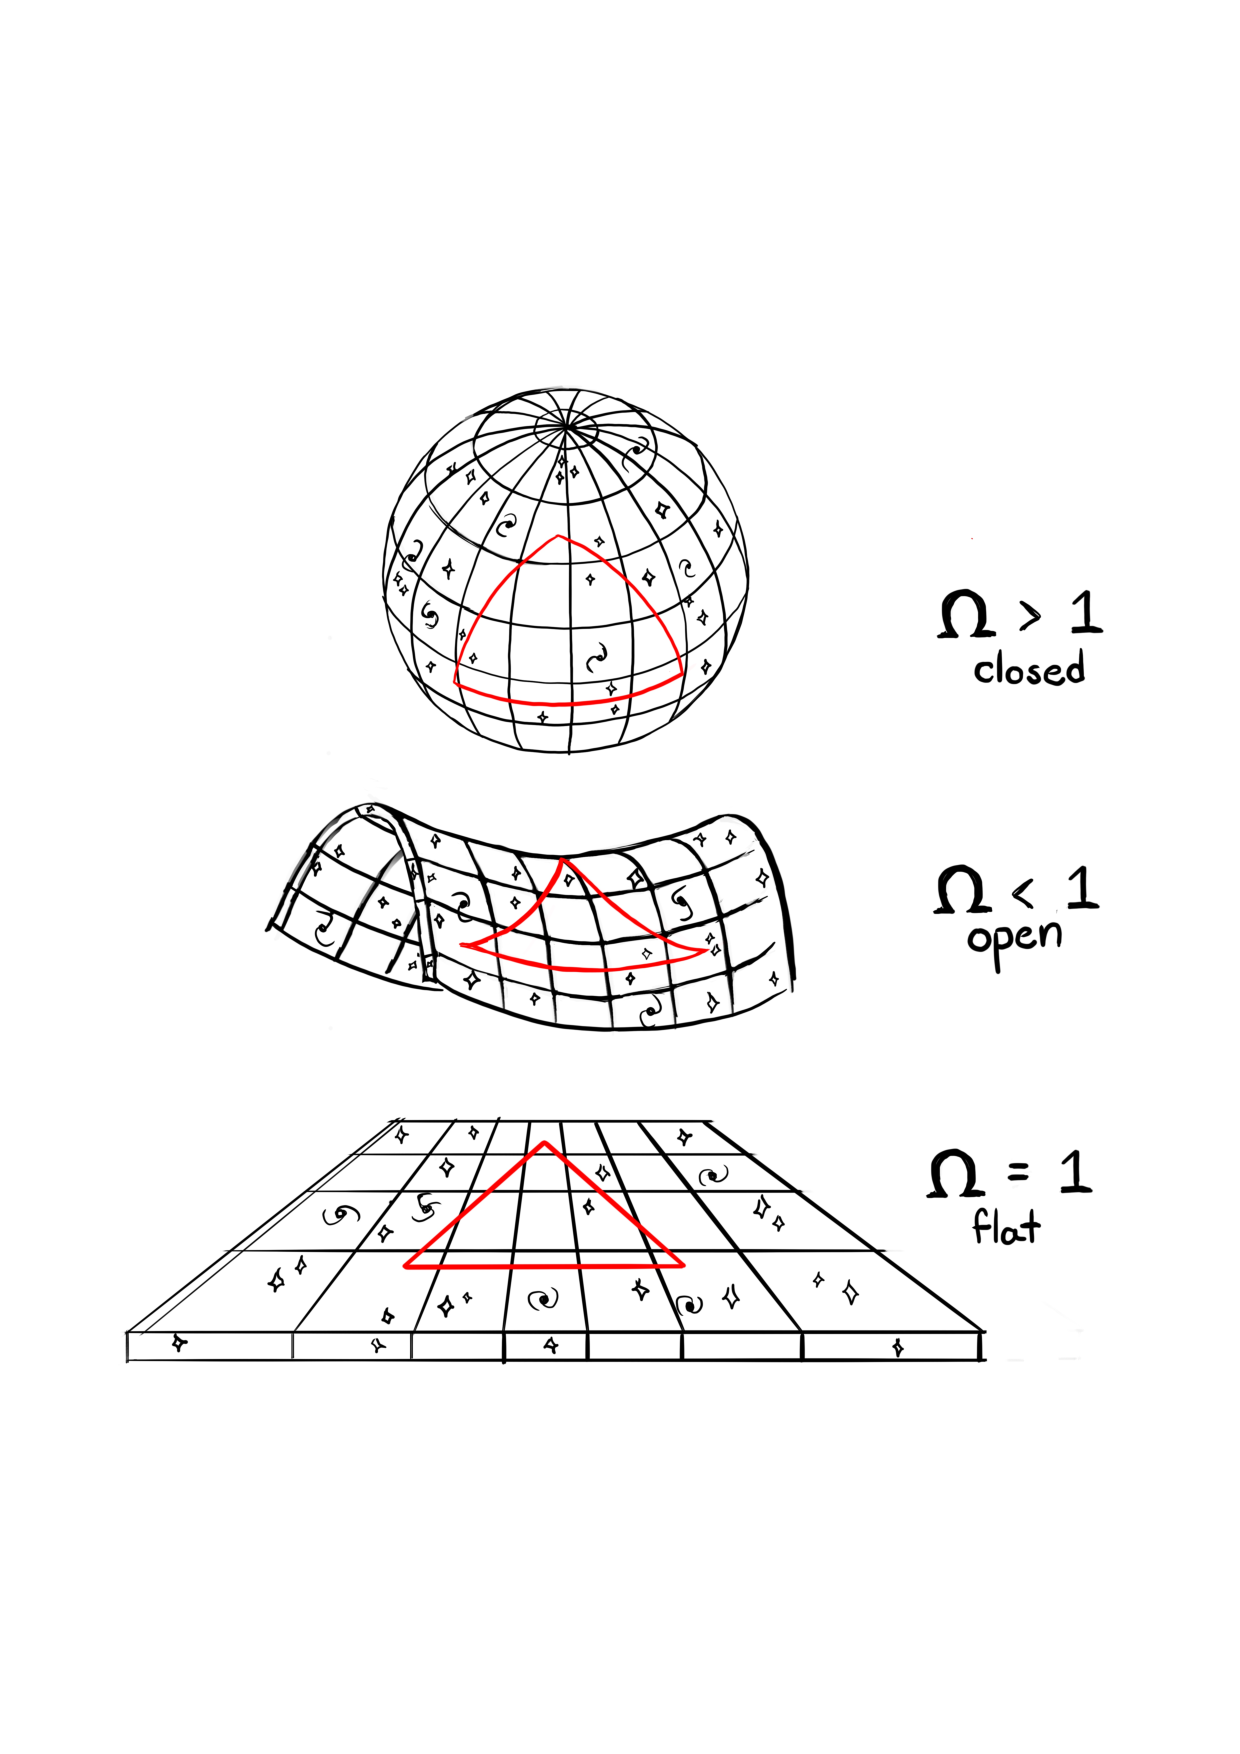
\includegraphics[width=\columnwidth]{Intro-FIGS/universeGeometry}
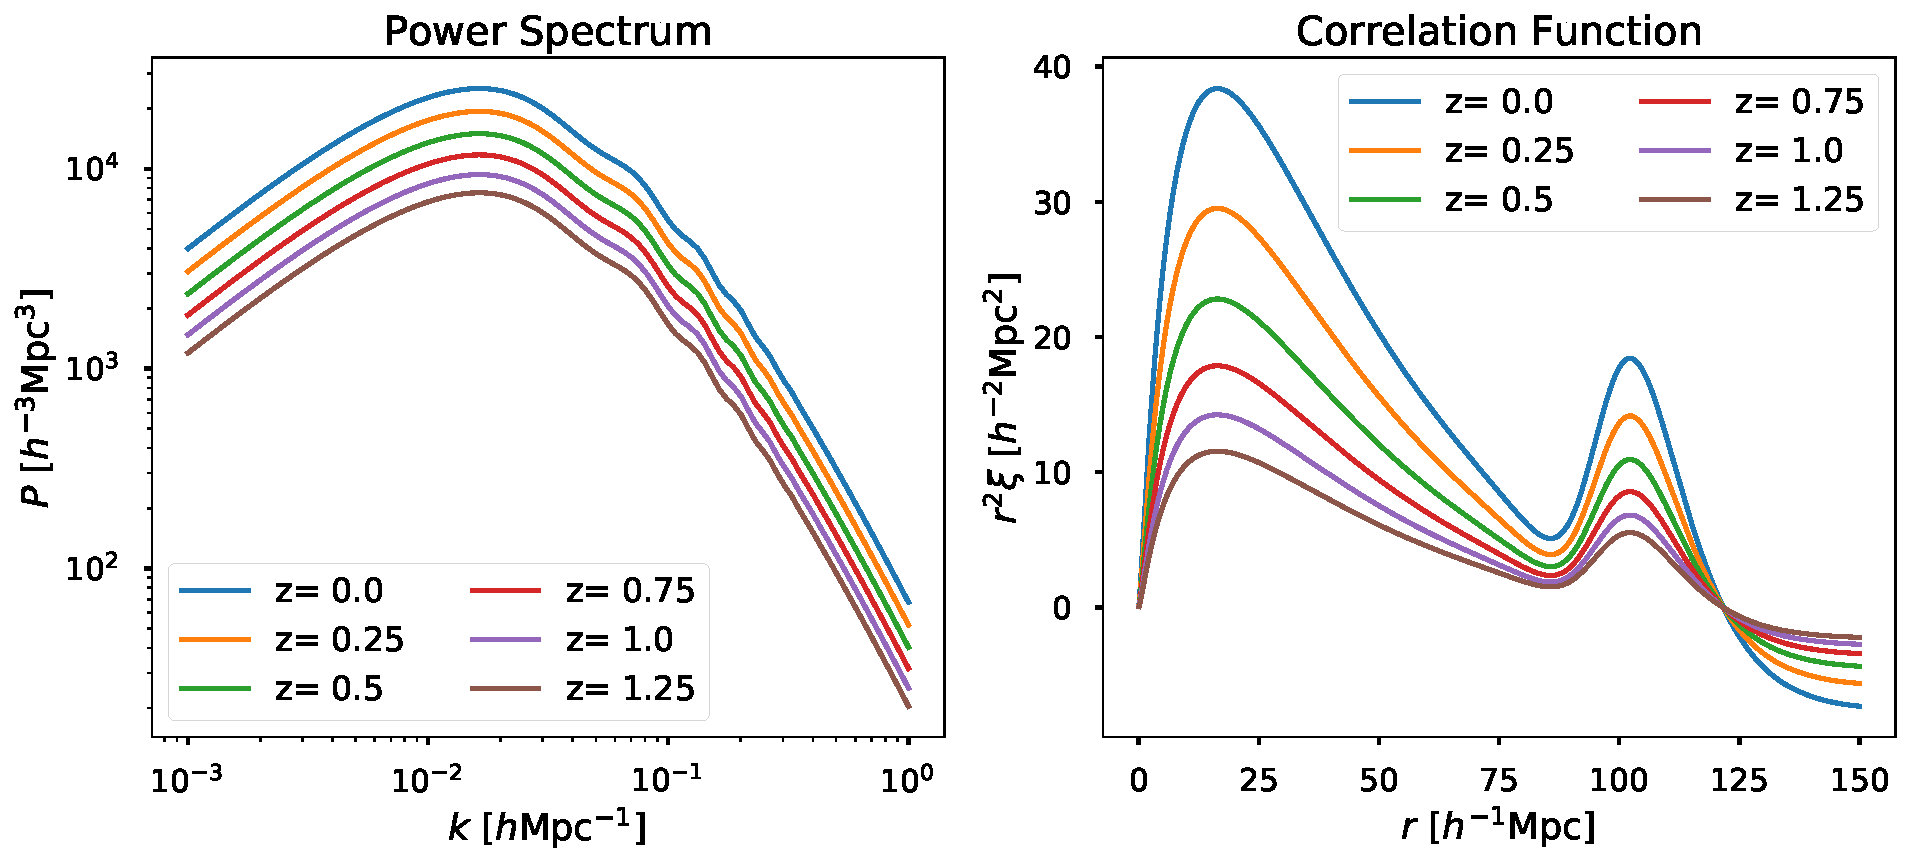
\includegraphics[width=\textwidth]{Intro-FIGS/Pk_Cf}
\caption[Power spectra and correlation functions calculated using the \class code.]{A series of power spectra and their Fourier counterparts, the correlation function, in different redshift ranges using a Planck 2015 fiducial cosmology \citep{PlanckResults2015} calculated using the \class code \citep{Class}. Note that the secondary peak in the correlation function (right) translates to wiggles in the power spectra (left), this is due to baryon acoustic oscillations in the primordial baryon-photon plasma.}
\label{fig:Pk_Cf}
\end{center}
\end{figure}

\qquad The growth factor determines the evolution of amplitude fluctuations in the Universe. A few approximations can be made in order to calculate this function and its redshift dependency; in a Newtonian approximation, for example, the growth function comes from solving the following differential equation \citep[][p. 345]{schneider_2016}:
\EQ{}{
\ddot{D}(z) + \frac{2\dot{a}}{a}\dot{D}-4\pi G \bar{\rho}(z)D(z) = 0 \, ,
}
which, in terms of the scale factor, has the following solution at late times \citep[][pages 206 and 345, respectively]{dods,schneider_2016}:

\EQ{}{
%D(a) = \frac{5\Omega_m}{2}\frac{H(a)}{H_0}\int_0^a \left( a' H(a')/H_0\right)^{-3}da'
D(a) = \frac{5\Omega_m}{2}\frac{H(a)}{H_0}\int_0^a \left[ \Omega_m/a' + \Omega_{\Lambda}a'^2 - (\Omega_m + \Omega_{\Lambda} -1 )\right]^{-3/2}da' \, ,}

where a convention of $D(z=0)=1$ was used. The impact of $D(z)$ in the two-point statistics can be see in Figure \ref{fig:Pk_Cf} for a fiducial $\Lambda$CDM model.
%\subsubsection{Galaxy bias and non-linear scales:}

\qquad Dark matter, however, does not interact electromagnetically with baryonic matter which complicates any attempts to directly measure fluctuations in the underlying matter density field. Although no direct dark matter observations were made so far \citep{2017DarkMatterExpReview}, matter tends to cluster due to gravity, i. e. both dark and baryonic matter interact gravitationally. This causes baryonic matter, in the form of galaxies, clusters of galaxies, intergalactic gas, and more to act as a biased tracer of the underlying matter overdensity field, $\delta_g = b\delta$ \citep{2000-BensonBias,1999Ofer-Bias}. This bias can be represented as a function of several different aspects of galaxies: luminosity \citep{2000-BensonBias,2004PVP,2013Baugh-LumBias}, scale \citep{1999Ofer-Bias,2008ScaleBias,2008Hamann-ScaleBias,2018Simon-ScaleBias}, galaxy type \citep{2008Sanchez-Bias,2016AbramoSeccoLoureiro}, and redshift \citep{1994FKP,1998Heavens-Verde,2000-BensonBias}. The underlying physics in this process is that more massive halos will form more massive galaxies, which will have different star formation histories, affecting mainly these before-mentioned aspects. The work presented in the subsequent sections and chapters, considers bias simply to be a function of redshift as a first order approximation. Therefore, its impact on the power spectrum of galaxy distributions, $P_g(k)$, is 

\EQ{}{
P_g(k,z) = b^2(z)P(k,z) \, .
}

\qquad Another important effect regarding probing the matter density field using galaxies as tracers is shot-noise. As the matter density field is a continuous field, the galaxy tracers are discrete objects which trace only regions with higher density. The discrete nature of this measurement leads to shot-noise in the measured power spectrum. If the survey contains a sufficient number of galaxies, the shot-noise can be approximately Poissonian, i. e. it can be expressed as the inverse number density of a given survey -- for the 3D power spectrum  \citep{1994FKP,2009Seljak-ShotNoise,2017Paech}. Details on how the shot-noise affects the angular power spectra of galaxies are outlined in Section \ref{Sec:Measurements}.

%%%%%%%%%%%%%%%%%%%%%%%%%%%%%%%%%%%%%%%%%%%%%%%%%%%%%%%%%%%
%				            BAO
%%%%%%%%%%%%%%%%%%%%%%%%%%%%%%%%%%%%%%%%%%%%%%%%%%%%%%%%%%%
\subsubsection{Baryon acoustic oscillations:}
The shape of both two-point statistics in Figure \ref{fig:Pk_Cf}, either in real or in Fourier space, raises attention to an interesting feature: the secondary peak in the correlation functions, manifested as wiggles in the power spectra. This peak is caused due to acoustic perturbation in the primordial baryon-photon plasma during radiation dominated era and are called baryon acoustic oscillations, or BAOs. Acoustic peaks were firstly observed in the CMB temperature angular power spectrum which raised the question if any similar features would appear in the large scale structure of galaxies. Using data from the 2-degree Field Galaxy Redshift Survey (2dFGRS), \cite{2001Percival} reported that their measurements of the 3D power spectra of galaxies `mildly preferred models where Baryon acoustic oscillations introduced wiggles in the $P_g(k)$ against a featureless power spectra'.Later, in 2005, two independent collaborations, SDSS and 2dFGRS, simultaneously reported measurements of the BAO peak. One of the measurements, carried out by the SDSS collaboration was performed using the 3D correlation function of luminous red galaxies (LRGs); detailes were presented in \cite{Einsenstein2005}. The other independent measurement, carried out by the 2dFGRS and presented in \cite{2005Cole-2dF}, was performed in Fourier space. Both compared the measured 2-pts statistics against a fiducial model with no Baryon acoustic oscillations and obtained a significant detection of this effect for late time cosmological probes.

%The tight coupling between baryons and photons in the primordial plasma during the radiation dominated era lead to what is called baryon acoustic oscillations, causing this peak to appear later on the statistical distribution of galaxies. These acoustic peaks were firstly observed in the CMB temperature angular power spectrum which raised the question if any consequences would appear in the large scale structure of galaxies. In \cite{Einsenstein2005}, this acoustic oscillations were first measured using the statistical distribution of SDSS luminous red galaxies (LRGs); the BAO peak was observed in the measured correlation function. 
\qquad The physical process behind the formation of BAO comes from the end of recombination era around $z \approx 1100$. The sound speed in the hot baryon-photon plasma decreased significantly and waves propagated due to the initial cosmological perturbations in this relativistic plasma. Baryons and photons were coupled both via Thompson scattering, gravitational attraction and radiation pressure; these couplings set up oscillations imprinting a characteristic length scale related to the oscillatory modes and the sound horizon at that epoch. Right after the period of recombination, the Universe goes through a period in which is non-ionised, `freezing' the baryonic oscillation scale while photons freely propagate. The density excess in the baryonic content of the Universe then interacts gravitationally with the non-coupled dark matter, later forming the distribution of galaxies with an imprinted acoustic peak.

\qquad Several fundamental conclusions, according to \cite{Einsenstein2005}, can be drawn from the BAO peak measurement. Initially, it provides very strong evidence that linear perturbation theory can be used in order to evolve the Einstein-Boltzmann equations (see Section \ref{Sec:Intro:LinTheory}) from redshift 1100 all the way to $z \approx 0$ -- at scales in which structure presents a linear behaviour. Another important conclusion comes from the interplay between dark and baryonic matter in order to form the BAO peak; a model with no dark matter present, purely baryonic, would not be able to reproduce the observed acoustic peak. Finally, the BAO peak provide cosmologists with a \textbf{standard ruler}, which can be measured over a wide range of redshifts, allowing us to probe the angular diameter distance along the line-of-sight together with the Hubble flow (Equation \ref{Eq:Intro:HubbleOmega1}). Currently, the most precise BAO measurements from galaxy surveys come from the BOSS Collaboration and are measured over a variety of methods -- see \citealt{2016BOSSCosmology} for a summary.

%%%%%%%%%%%%%%%%%%%%%%%%%%%%%%%%%%%%%%%%%%%%%%%%%%%%%%%%%%%
%		        	NON-LINEAR THEORY
%%%%%%%%%%%%%%%%%%%%%%%%%%%%%%%%%%%%%%%%%%%%%%%%%%%%%%%%%%%
\subsubsection{The non-linear power spectra:}
When dealing with smaller scales, at the order of clusters of galaxies, the linear theory approximation starts leading to imprecision in the power spectrum calculation. This is mostly due to the overdensity field's module tending to unity, which breaks down perturbation theory assumptions. Instead, different approaches are necessary. Computational calculation of non-linear overdensity amplitude fluctuations is usually performed with the use of N-body simulations with a wide range of cosmological parameters and fitting these to obtain power spectra predictions. The most used fitting is \texttt{HALOFIT} \citep{2003HaloFit,2012-Halofit,Bird2012} and its impact in the measured power spectra can be seen as an increase of power in smaller scales. Although a lot of collective effort has been put into perfecting these calculations over the years, as a rule of thump, the non-linear power spectrum is used to perform scale cuts in cosmological analyses\footnote{See Section \ref{Sec:CosmoAnal} in Chapter \ref{Chap:BOSS-Cosmo} for an example.} as even the latest advances on \texttt{HALOFIT} have around 5\% precision on scales up to $k\leq 1$ h/Mpc in $0\leq z \leq 10$ \citep{2012-Halofit,Bird2012}. 

%%%%%%%%%%%%%%%%%%%%%%%%%%%%%%%%%%%%%%%%%%%%%%%%%%%%%%%%%%%
%				WEAK LENSING
%%%%%%%%%%%%%%%%%%%%%%%%%%%%%%%%%%%%%%%%%%%%%%%%%%%%%%%%%%%
\subsection{Weak Lensing}
One of the earliest predictions from the General Theory of Relativity was that gravity should cause light to be distorted in specific ways, differently from what was predicted by Newtonian theory. Later, in 1919, by observing the background light of stars distorted by the Sun during an eclipse, this effect was confirmed in an expedition led by Sir Frank Dyson and Sir Arthur Eddington to Sobral in Brazil and the island of Principe in the African coast \citep{Dyson291}. Although some of the photosensitive plates from Eddignton's expedition to the island of Principe were compromised due to bad weather conditions, the ones taken in Sobral where more than sufficient to demonstrate that General Relativity passed its first ever test \citep{2007arXiv0709.0685K}.


\qquad Years after the eclipse, it is well known from General Relativity and observations that gravity causes light to bend like it does in the presence of lenses. One of the most impressive facts about this effect is that it allows for a reconstruction of dark matter's distribution even without the ability to properly observe it. As light is bend by matter, so it is by dark matter which deflects and distorts the shapes and sizes of background galaxies in relation to a massive foreground like a cluster. In first order, the lensing effects can be summarised by two phenomena: an isotropic dilatation called convergence, $\kappa$, and an anisotropic distortion called shear, $\gamma$. 

\qquad To understand these effects, one starts from an approximation of the lens equation -- which relates the true angle between an observer and an object, $\theta_{\text{src}}$, and the observed angle in the sky due to the bending of light, $\theta_{\text{obs}}$ \citep[][p. 296]{dods}:

\EQ{}{
\theta_{\text{src},i} = A_{ij}\theta_{\text{obs},j}\, .
}
Here, the Jacobian matrix A can be related to convergence $\kappa$, the shear components $\gamma_1$ \& $\gamma_2$, and the Newtonian potential, $\Phi$, as

\EQ{}{
A_{ij} - \delta_{ij} = \left( \begin{matrix}
							- \kappa - \gamma_1 & -\gamma_2 \\
                             -\gamma_2  & -\kappa + \gamma_1
							\end{matrix} \right) 
                            = 2\int_0^{\chi}d\chi ' \Phi_{,ij}(\chi'\theta_{\text{obs}})\chi'\left(1-\frac{\chi'}{\chi}\right)\, ,
}
where $\chi$ is the comoving distance to the source and $\gamma^2 = \gamma_1^2 + \gamma_2^2$. In terms of observables, both shear and convergence can be estimated using a combination of measurements from galaxy ellipticities and mass surface projections. When observing the ellipticity of a galaxy, both shear and the intrinsic ellipticity are being measured. The intrinsic ellipticity is expected to be random \footnote{In first order. However, a lot of work has been done into understanding the role of the environment a galaxy is immerse in intrinsic alignments. See \cite{2015Kirk_IA} for a review.} and is averaged out when measured over enough background galaxies. 

\qquad Several galaxy surveys like DES \citep{2017arXiv170801530D}, KiDS \citep{2017MNRAS.465.1454H}, and CHFTLens \citep{2014CHFTLens} are focused in using weak lensing measurements for extracting cosmology, combining with galaxy clustering, producing mass maps of the dark matter field, between other applications. Chapter \ref{Chap:BPL} has a general discussion on measuring shear and polarisation power spectra from photometric galaxy surveys and CMB polarisation measurements as spin-2 fields. For a more general review on weak gravitational lensing methods, measurements, and theory please see \cite{2005astro.ph..9252S} and \cite{2017SchpJ..1232440B}.

% \begin{itemize}
% \item Lensing potential
% \item Shear power spectrum
% \item Convergence
% \end{itemize}

%%%%%%%%%%%%%%%%%%%%%%%%%%%%%%%%%%%%%%%%%%%%%%%%%%%%%%%%%%%
%				BAYESIAN STATIS
%%%%%%%%%%%%%%%%%%%%%%%%%%%%%%%%%%%%%%%%%%%%%%%%%%%%%%%%%%%
\section{Bayesian Statistics Applied to Cosmology}\label{sec:intro:motivation}
Data analysis is at the core of the contemporary approach to cosmology. With the construction of bigger and more powerful telescopes, the amount of cosmological data present is increasing at an unprecedented rate. Such a great amount of data cannot be analysed via `brute force' methods and compression of information is key, evoking the need of advanced statistical analysis methods. Cosmology is unlike most sciences, the nature of our object of study is unique: the Universe. Cosmologists do not have the `luxury of turning the experiment's machine on and off again' in order to reproduce different realisations of the data; there is only one Universe, implying that common statistical approaches (like a frequentist approaches) are insufficient.

\qquad There are countless applications for Bayesian statistics in cosmology, ranging from photometric redshift estimations, cosmological parameter estimation, alternative ways to measure the power spectrum, and many more -- the last two are subjects of chapters in this work. In this section, I will focus on the application of Bayesian statistics to cosmological parameter estimation with a generic approach. Chapter \ref{Chap:BPL} presents an application to angular power spectra estimation.


\subsection{Bayes' Theorem and Marginalisation}
In cosmology, as in any other science, we want to be able to assert statements and hypothesis, assigning them `degrees of plausibility' which can be represented by `rules of probability' for consistent reasoning \citep{sivia2006data}. These can be represented, initially, by a very simple set of arguments:
\begin{enumerate}
\item Probabilities can be expressed by real numbers:
\EQ{}{
\Pr(\text{True}) = 1 \quad \text{as} \quad \Pr(\text{False}) = 0.
}
\item The probability of a certain hypothesis A increases as the probability of `not-A', or $\bar{A}$, decreases:
\EQ{Intro:Sum}{
\Pr(A|M) = 1 - \Pr(\bar{A}|M).
}
This is also known as the `sum rule'; while M is the model or any underlying assumption made.
\item Two hypothesis can be related via a join hypothesis where the probability of A given B is expressed as:
\EQ{Intro:Product}{
\Pr(A,B|M) = \Pr(A|B,M)\Pr(B|M).
}
This expression is commonly known as `the product rule'.
\item The degrees of plausibility should be transitive in a sense that if A is more probable than B; B is more probable than C; than A is unquestionably more probable than C.

\item These plausibilities are independent of the order in which they are considered, depending only on the available data.
\end{enumerate}

%%%%%%%%%%%%%%%%%%%%%%%%%%%%%%%%%%%%%%%%%%%%%%%%%%%%%%%%%%%
%				DROP THE BAYES
%%%%%%%%%%%%%%%%%%%%%%%%%%%%%%%%%%%%%%%%%%%%%%%%%%%%%%%%%%%
\subsubsection{Bayes' Theorem:}
\qquad In Bayesian statistics, the degree of plausibility is expressed in terms of a \textbf{posterior distribution}. This distribution relates the likelihood distribution to prior knowledge and the current evidence. Using both the sum and product rules, Bayes' theorem can be expressed as
\EQ{Intro:Bayes}{
\Pr(A|B,M) = \frac{\mathcal{L}(B|A, M)\Pi(A|M)}{\mathcal{Z}(B|M)}\, ,
}
where $\mathcal{L}(B|A, M)$ is the likelihood, the probability of the acquiring the data, B, given hypothesis A and model M; $\Pi(A|M)$ is the prior distribution, which is the probability of hypothesis A given prior knowledge on the model M; finally, $\mathcal{Z}(B|M)$, the normalisation factor or evidence, is the probability of the data given the model only. The combination of these probability distribution functions (p.d.f.) leads to the posterior distribution, the plausibility of the hypothesis given the data and the underlying assumptions about the model. 

\qquad In other words, Bayes' theorem relates the probability over the veracity of a certain hypothesis given the data, to the probability that the data could have been measured in case where the hypothesis is true. This is the information encompassed into the likelihood function. However, it is the prior which differentiate Baysian statistics from the usual frequentist approach: it allows for previous knowledge to be incorporated into the assessment of the hypothesis's veracity. The prior distribution exhibit how much is known or unknown about the hypothesis' truth assertion before any data are analysed. 

%%%%%%%%%%%%%%%%%%%%%%%%%%%%%%%%%%%%%%%%%%%%%%%%%%%%%%%%%%%
%				MARGINALISATION
%%%%%%%%%%%%%%%%%%%%%%%%%%%%%%%%%%%%%%%%%%%%%%%%%%%%%%%%%%%
\subsubsection{Marginalisation and nuisance parameters:}
One of many advantages of Bayesian statistics is the possibility of dealing with parameters which need to be probed but are not of any particular interest, these are called `nuisance parameters'. In cosmology, nuisance parameters range from a instrumental calibration parameters to galaxy bias and redshift errors. Marginalisation is the key concept to deal properly with undesired parameters, and it is done by accounting for all possibilities related to the these parameters. Consider now a nuisance parameter, or hypothesis, B. One can account for it as a nuisance parameter by adding the probability of $\bar{B}$ in Equation \eqref{Eq:Intro:Product}:
\EQ{}{
\Pr(A,B|M) + \Pr(A,\bar{B}|M) = \left[ \Pr(B|A,M) + \Pr(\bar{B}|A,M)\right]\Pr(A|M),
}
where, with the use of Equation \eqref{Eq:Intro:Sum} the expression in brackets is unity in the above expression leading to
\EQ{}{
\Pr(A|M) = \Pr(A,B|M) + \Pr(A,\bar{B}|M)\, ,
}
meaning that the probability that the hypothesis A is true, independently of B being true, is the sum of probabilities of A and B being true plus A being true while B is not. Generally speaking, this expression translates to
\EQ{}{
\Pr(A|M) = \int_{-\infty}^{+\infty}\Pr(A,B|M)dB\, .
}

\qquad This method has a wide range of applications. An example of its power is that it allows for a much higher dimensional posterior, with a much simpler way to sample from, to be probed at the higher dimensional space and then marginalised over the dimensions of interest. A similar application is explored in Chapter \ref{Chap:BPL} for sampling from the joint distribution of spherical harmonics and angular power spectra, marginalising over the spherical harmonics coefficients, and obtaining a posterior for the power spectra of galaxy clustering.

%%%%%%%%%%%%%%%%%%%%%%%%%%%%%%%%%%%%%%%%%%%%%%%%%%%%%%%%%%%
%				DISFARÇAR AS EVIDENCIAS
%%%%%%%%%%%%%%%%%%%%%%%%%%%%%%%%%%%%%%%%%%%%%%%%%%%%%%%%%%%
\subsection{Evidence and Bayes Factor for Model Selection}
Although controversial in some aspects, the Bayesian evidence can be used to assess model selection. Treated as a normalisation factor for a long time, mostly due to the complications in calculating it, the evidence is an important piece of the Bayesian inventory and it is a natural by-product of nested sampling (discussed in more detail in Section \ref{Sec:Sampling}). Evidence calculations are more robust when their ratios are considered -- these are usually referred to as `Bayes factors',
\begin{equation}
R_{A,B} = \frac{\mathcal{Z}(A|M)}{\mathcal{Z}(B|M)}
\label{Eq:Intro:BayesFactor}
\end{equation}
where here A and B can either be hypothesis or datasets. 

\qquad Another application for the Bayes factor is to assess consistency between combining two or more datasets. Considering three datasets, A, B, and C, the Bayes factor for combining these given a model M is
\begin{equation}
R_{A,B,C} = \frac{\mathcal{Z}(A,B,C|M)}{\mathcal{Z}(A|M)\mathcal{Z}(B|M)\mathcal{Z}(C|M)}
\label{Eq:Intro:BayesFactor2}
\end{equation}
which, if much bigger than unity, favours the combination of datasets. 

\qquad As outlined in Chapter \ref{Chap:BOSS}, this method of model selection has received several criticisms in the late years as values for the Bayes factor can have strong dependencies on the prior volume for each case. However, physically motivated priors should lead to reliable values for the Bayes factor, being then a reflection of the true consistency between datasets. Nonetheless, a plethora of new methods for model selection and dataset consistency assessment have been proposed by the community in the past few years. I have not explored this techniques in this work. For an investigation of a few of these new methods, please refer to \cite{2017CharnockTension,2018HuTension,2018FeeneyTension}.

%%%%%%%%%%%%%%%%%%%%%%%%%%%%%%%%%%%%%%%%%%%%%%%%%%%%%%%%%%%
%			    	PARAM_EST
%%%%%%%%%%%%%%%%%%%%%%%%%%%%%%%%%%%%%%%%%%%%%%%%%%%%%%%%%%%
\subsection{Parameter Estimation}\label{Sec:ParamEstSampling}
For a certain dataset, information regarding a given parameter's degree of plausibility is contained within the posterior distribution. A common way to summarise this information is via quoting best-fit points and confidence intervals (CI) or via a mean and a standard-deviation. The probability density of certain parameter's value is an evaluation of reliability that the true value is near the estimated one; this is usually given by the maximum of the posterior probability distribution function.

\qquad Consider $\{\theta_i\}$ to be the set of parameters in interest, $\vec{D}$ to be the data vector, M to be the model, and $\mathcal{P} = \Pr(\{\theta_i\}|\vec{D}, M)$ the posterior distribution. The set of best-fit estimates, $\Theta_{0,i}$, should be found near the maximum, i. e.
\EQ{}{
\left. \frac{\partial \mathcal{P}}{\partial \theta_i} \right\rvert_{\Theta_{0,i}} = 0
\quad \text{and} \quad
\left. \frac{\partial^2 \mathcal{P}}{\partial \theta_i^2} \right\rvert_{\Theta_{0,i}} < 0
}

\qquad For flat priors, the best estimates can be expressed mostly in terms of the log-likelihood, $\mathbb{L} = \ln \mathcal{L}(\vec{D}|\{\theta_i\},M)$, where 
\EQ{}{
\left. \frac{\partial \mathbb{L}}{\partial \theta_i} \right\rvert_{\Theta_{0,i}} = 0.
}
This log-likelihood can now be Taylor expanded into
\EQ{}{
\mathbb{L} = \mathbb{L}(\Theta_{0,i}) + \frac{1}{2} \sum^{N}_{i=1}\sum^{N}_{j=1} \left.\frac{\partial^2 \mathbb{L}}{\partial \theta_i \partial \theta_j} \right\rvert_{\Theta_{0,i}} (\theta_i - \Theta_{0,i}) (\theta_j - \Theta_{0,j}) + ...
}
Following, using a matrix notation in the Taylor expansion's first term, the likelihood takes a more familiar form,
\EQ{}{
\Pr(\bm{\theta}|\vec{D},M)\propto \exp\left[-\frac{1}{2}(\bm{\theta} - \mathbf{\Theta}_0)^T\bm{\nabla\nabla}\mathbb{L}(\mathbf{\Theta}_0)(\bm{\theta} - \mathbf{\Theta}_0)  \right] \, ,
}
a multivariate Gaussian distribution where the $N\times N$ matrix of second derivatives is known as the Hessian, $\bm{\nabla\nabla}\mathbb{L}(\mathbf{\Theta}_0)$. The Fisher information matrix is related to the Hessian as its expectation value -- and, consequently, it is also related to the covariance matrix:
\EQ{}{
\mathcal{F}_{ij} = \langle-(\bm{\nabla\nabla}\mathbb{L})_{ij}\rangle = \text{Cov}^{-1}_{ij}\, .
}
However, the Cram\'er-Rao theorem affirms that this equality only holds if the estimated best-fit value is truly at the maximum posterior for a multivariate Gaussian, otherwise $\text{Cov}_{ij} \geq \mathcal{F}^{-1}_{ij}$. Section \ref{Sec:LikelihoodsPriors} gets into the cosmological parameter estimation problem in more details.

%%%%%%%%%%%%%%%%%%%%%%%%%%%%%%%%%%%%%%%%%%%%%%%%%%%%%%%%%%%
%				MC MONTE-CARLO
%%%%%%%%%%%%%%%%%%%%%%%%%%%%%%%%%%%%%%%%%%%%%%%%%%%%%%%%%%%
\subsection{Monte-Carlo techniques for Bayesian inference}\label{Sec:Sampling}
Given the sizes of current data vectors in cosmology, a `brute force method' involving an N-dimensional grid interpolation of the posterior function in parameter space is completely out of question; an alternative method is necessary. Monte-Carlo techniques are a quick and reliable way to explore the posterior distribution's peaks and tails in a multi-dimensional space. Several different Monte-Carlo sampling techniques are widely used in cosmology where the main idea is to perform some sort of random walk in parameter space while attempting to probe the posterior distribution. 

\qquad Next, I will outline some examples of sampling techniques that are relevant for this work.

\subsubsection{Metropolis-Hastings:}
Metropolis-Hastings (MH) is one of the most common sampling techniques adopted by the cosmological community \citep{2002CosmoMC}. Even though I do not make use of this technique in this work, outlining it has a pedagogical importance as it sets the grounds for being one of the simplest sampling techniques to implement -- which also explains its popularity. In this algorithm, the walk in parameter space happens when the chain jumps from an initial position in parameter space, $\bm{\theta}_n$, to a following position, $\bm{\theta}_{n+1}$, with a transition probability function, $T(\bm{\theta}_n,\bm{\theta}_{n+1})$. This transition probability function ensures that the chain will have an asymptotic distribution that reflects the posterior's distribution. The selection of a new point is performed with the help of a proposal density distribution, $G(\bm{\theta}_n, \bm{\theta}_{n+1})$, which defines the new point based on the previous one. The new point is then accepted with a probability
\EQ{}{
\gamma(\bm{\theta}_n, \bm{\theta}_{n+1}) = \min \left\lbrace 1, \frac{\Pr(\bm{\theta}_{n+1}|\vec{D},M)G(\bm{\theta}_{n+1}, \bm{\theta}_{n})}{\Pr(\bm{\theta}_{n}|\vec{D},M)G(\bm{\theta}_n, \bm{\theta}_{n+1})} \right\rbrace \,
}
where here $T(\bm{\theta}_n,\bm{\theta}_{n+1}) = \gamma(\bm{\theta}_n, \bm{\theta}_{n+1})G(\bm{\theta}_n, \bm{\theta}_{n+1})$ guaranteeing that the sampled posterior is the Markov Chain equilibrium distribution:
\EQ{}{
\Pr(\bm{\theta}_{n+1}|\vec{D},M)T(\bm{\theta}_{n+1},\bm{\theta}_{n}) = \Pr(\bm{\theta}_{n}|\vec{D},M)T(\bm{\theta}_{n},\bm{\theta}_{n+1})\, .
}
This also ensures correlations between accepted points. The method converges purely with $n\rightarrow \infty$, but acceptable convergence naturally occurs with a finite number of samples.

\subsubsection{Hamiltonian Monte-Carlo:}
Although MH is a very simple technique to implement, it has several limitations and it can be extremely time consuming if the number of dimensions increase. Hamiltonian Monte-Carlo (HMC) is a more sophisticated technique and it samples the posterior considering the evolution of Hamilton's equations -- which explains the name \citep{Taylor2008}. In this algorithm, consider the potential energy $\psi$ of a posterior distribution $\Pr(\bm{x})$ as the negative log-posterior,
\EQ{Intro:Pot_HMC}{
\psi(\bm{x}) = - \log\Pr(\bm{x}) \, .
}
In the expression above, $\bm{x}$ is the N-dimensional vector of parameters to be sampled, $x_i$. Each of the parameters are assigned to a momentum, $p_i$, and mass, $m_i$, such that the kinetic energy of this system of parameter-particles is defined as
\EQ{Intro:K_HMC}{
\phi(\bm{p}) = \sum_i^N \frac{p_i^2}{2m_i}\, .
}

\qquad Now, one can define the Hamiltonian of the system by using the potential and kinetic energies,
\EQ{}{
\mathcal{H}(\bm{x},\bm{p}) = \sum_i^N\frac{p_i^2}{2m_i} + \psi(\bm{x}) \, .
}
The main idea in this method is to sample from a distribution proportional to $\exp(-\mathcal{H})$ which can be expressed as
\EQ{Intro:HMC_ExpH}{
\exp(-\mathcal{H})\propto \Pr(\bm{x})\prod_i^N\exp\left(-\frac{1}{2}\frac{p_i^2}{m_i}\right)\, .
}

\qquad The distribution in Equation \eqref{Eq:Intro:HMC_ExpH} is now separated into a posterior distribution and a Gaussian containing the parameters' momenta. Now, one can marginalise over the momenta parameters while sampling at each new step -- as the momenta are nuisance parameters. To generate a new posterior sample, one starts by drawing a sample from the kinetic energy distribution -- an uncorrelated normal distribution with zero mean and a variance equal to the masses of the parameters. Starting with an initial point $(\bm{x}, \bm{p})$, this system can now be deterministically evolved using a fixed time parameter, $t$. A new point $(\bm{x}', \bm{p}')$ is found by evolving Hamilton's equations,
\EQ{Intro:HMC_Hamil}{
\frac{dx_i}{dt} & = \frac{\partial\mathcal{H}}{\partial p_i}\, ,\\
\frac{dp_i}{dt} & = -\frac{\partial \mathcal{H}}{\partial x_i} = -\frac{\partial \psi(\bm{x})}{\partial x_i} \, ,
}
where a new point is accepted with probability $\gamma(\bm{x}, \bm{x}', \bm{p}, \bm{p}') = \min(1, exp(-\delta\mathcal{H}))$ and $\delta\mathcal{H}$ is the change in the Hamiltonian between the previous point and the proposed new one: $\delta\mathcal{H} = \mathcal{H}(\bm{x}, \bm{p}) - \mathcal{H}(\bm{x}', \bm{p}')$. If the trajectory conserves energy, than $\delta\mathcal{H} = 0$ and $\gamma =1$, so the point is accepted. 

\qquad More details in how to evolve Hamilton's equations for this algorithm and a extension to much higher dimensional problems are explored in Section \ref{Sec:BPL:GHS}.

\subsubsection{Nested Sampling:}
In the past few years, Nested Sampling's popularity is increasing considerably within the cosmological community. Its ability to sample the posterior while probing the evidence allows for both parameter estimation and model selection simultaneously \citep{2004NestedSampling}. This algorithm --although containing different variations like \texttt{MultiNest} \citep{2009Multinest}, \texttt{PolyChord} \citep{2015PolyChord}, and \texttt{Pliny} \citep{PlinyRichardThesis} -- has a simple idea based in using a collection of $n_{\text{live}}$ objects $\bm{\theta}$, called `live-points', which were sampled from the prior distribution, but are constrained to be inside a certain value of the likelihood, $\mathcal{L}(\bm{\theta}) > \mathcal{L}^*$ \citep{sivia2006data}.

\qquad Firstly, the N-dimensional parameter prior space, $\Pi(\bm{\theta}|M)$, is transformed into a N-dimension unity cube. The live-points are randomly sampled within the prior volume subjected to a constrain related to $\mathcal{L}^*$:
\EQ{Intro:PriorVolume}{
\xi(\mathcal{L}^*) = \idotsint_{\mathcal{L}(\bm{\theta}) > \mathcal{L}^*} \Pi(\bm{\theta}|M)d\bm{\theta} \, .
}
All points are drawn within this space and their likelihoods are evaluated. The likelihood values are used to assess if a live-point is inside an iso-contour $\mathcal{L} = \mathcal{L}^*$, for a given $\mathcal{L}^*\geq 0$. The point with the lowest likelihood, $\mathcal{L}_{\min}$, is then identified and eliminated and a new point is drawn inside the $\mathcal{L} = \mathcal{L}_{\min}$ iso-contour. This process is repeated until the maximum likelihood value is found, always identifying likelihood iso-curvatures at each step until the final peak is found.

\qquad Using this sampling technique, the evidence can be estimated simply by calculating
\EQ{}{
\mathcal{Z} = \int_0^1\mathcal{L}(\xi)d\xi
}
which becomes much simpler to evaluate in this algorithm as one does not need now to evaluate a N-dimensional integral, which, in this case is simply a Riemann sum of the weights.

%%%%%%%%%%%%%%%%%%%%%%%%%%%%%%%%%%%%%%%%%%%%%%%%%%%%%%%%%%%
%			            SURVEYS
%%%%%%%%%%%%%%%%%%%%%%%%%%%%%%%%%%%%%%%%%%%%%%%%%%%%%%%%%%%
\section{State-of-the-art Cosmological Probes}\label{sec:intro:probes}
In this section I will outline some of the state-of-the-art past, current, and future surveys used in the following chapters -- either to extract cosmological information from, or to forecast future cosmological endeavours.

\subsection{Planck Satellite}
\begin{figure}
\begin{center}
%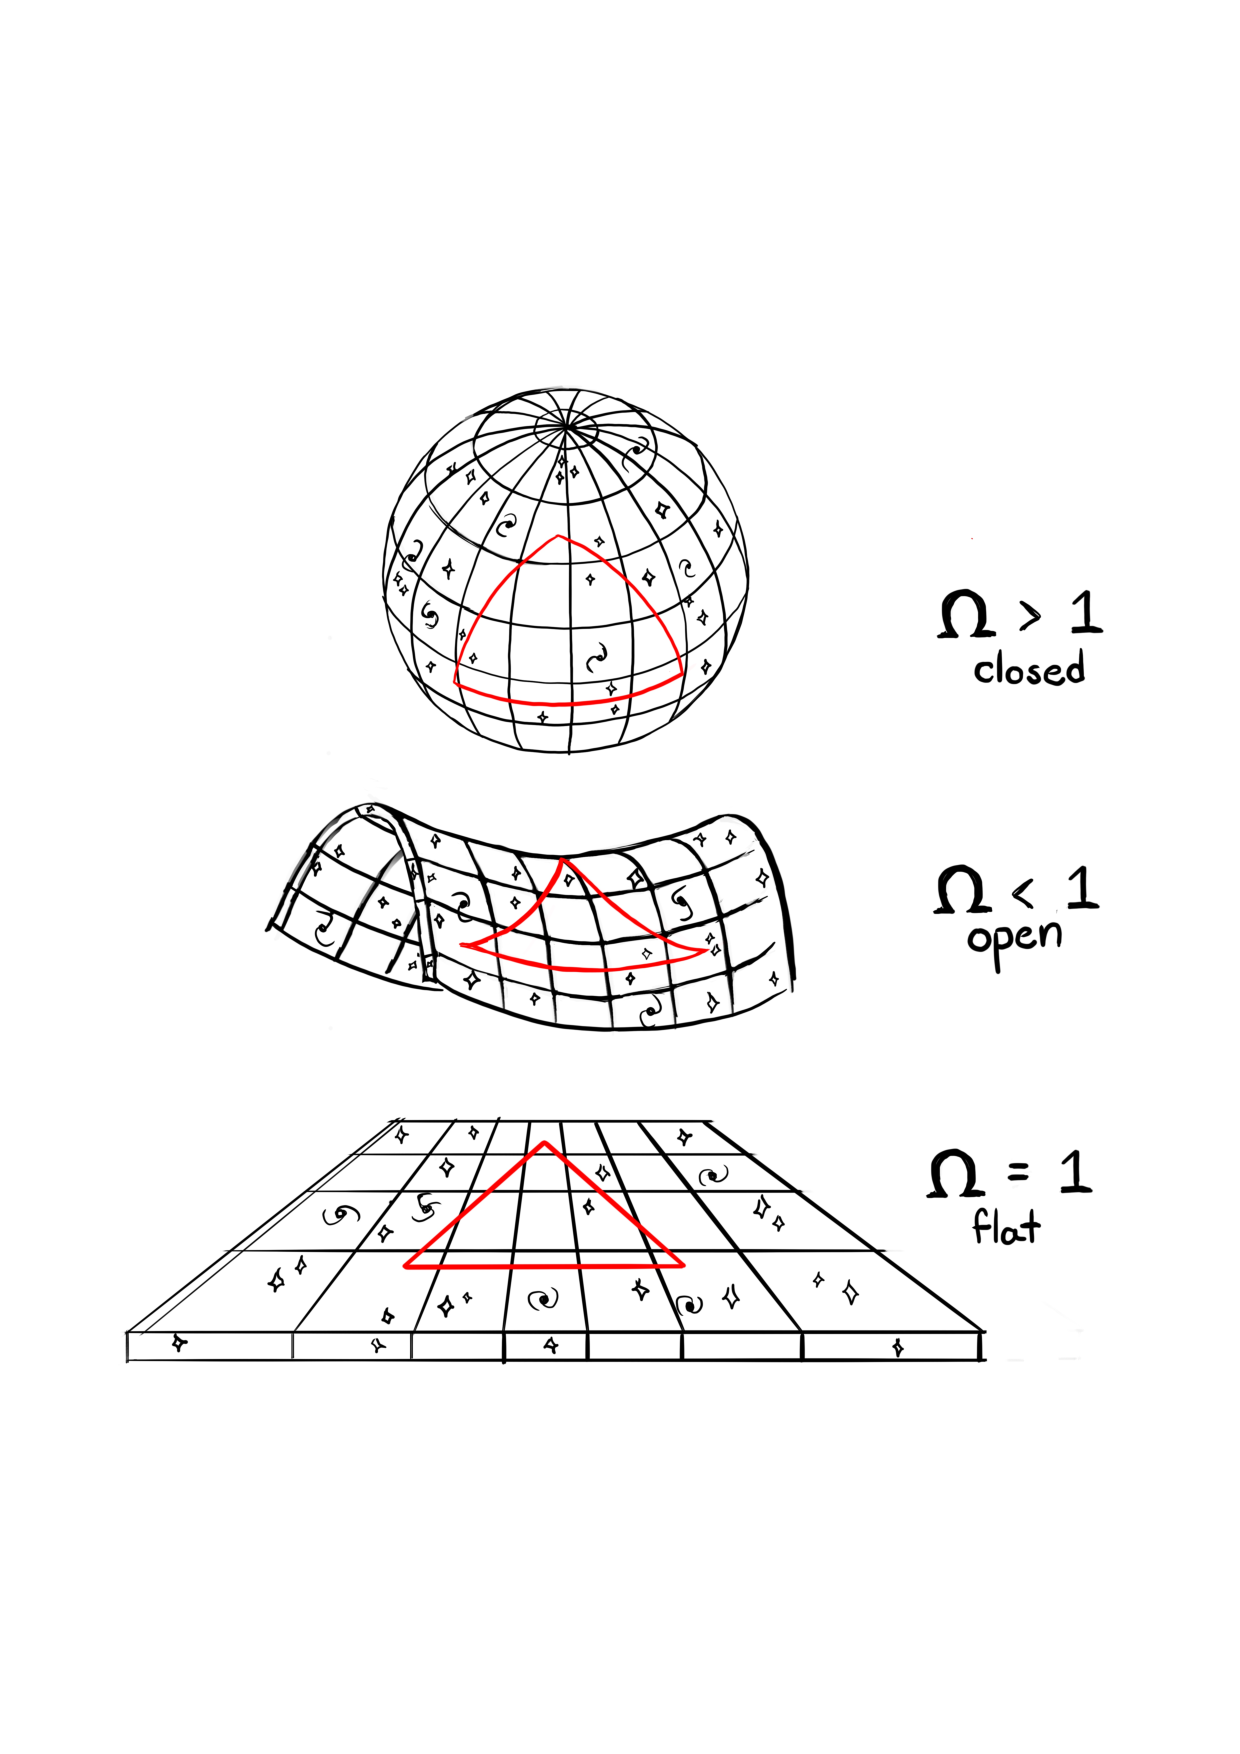
\includegraphics[width=\columnwidth]{Intro-FIGS/universeGeometry}
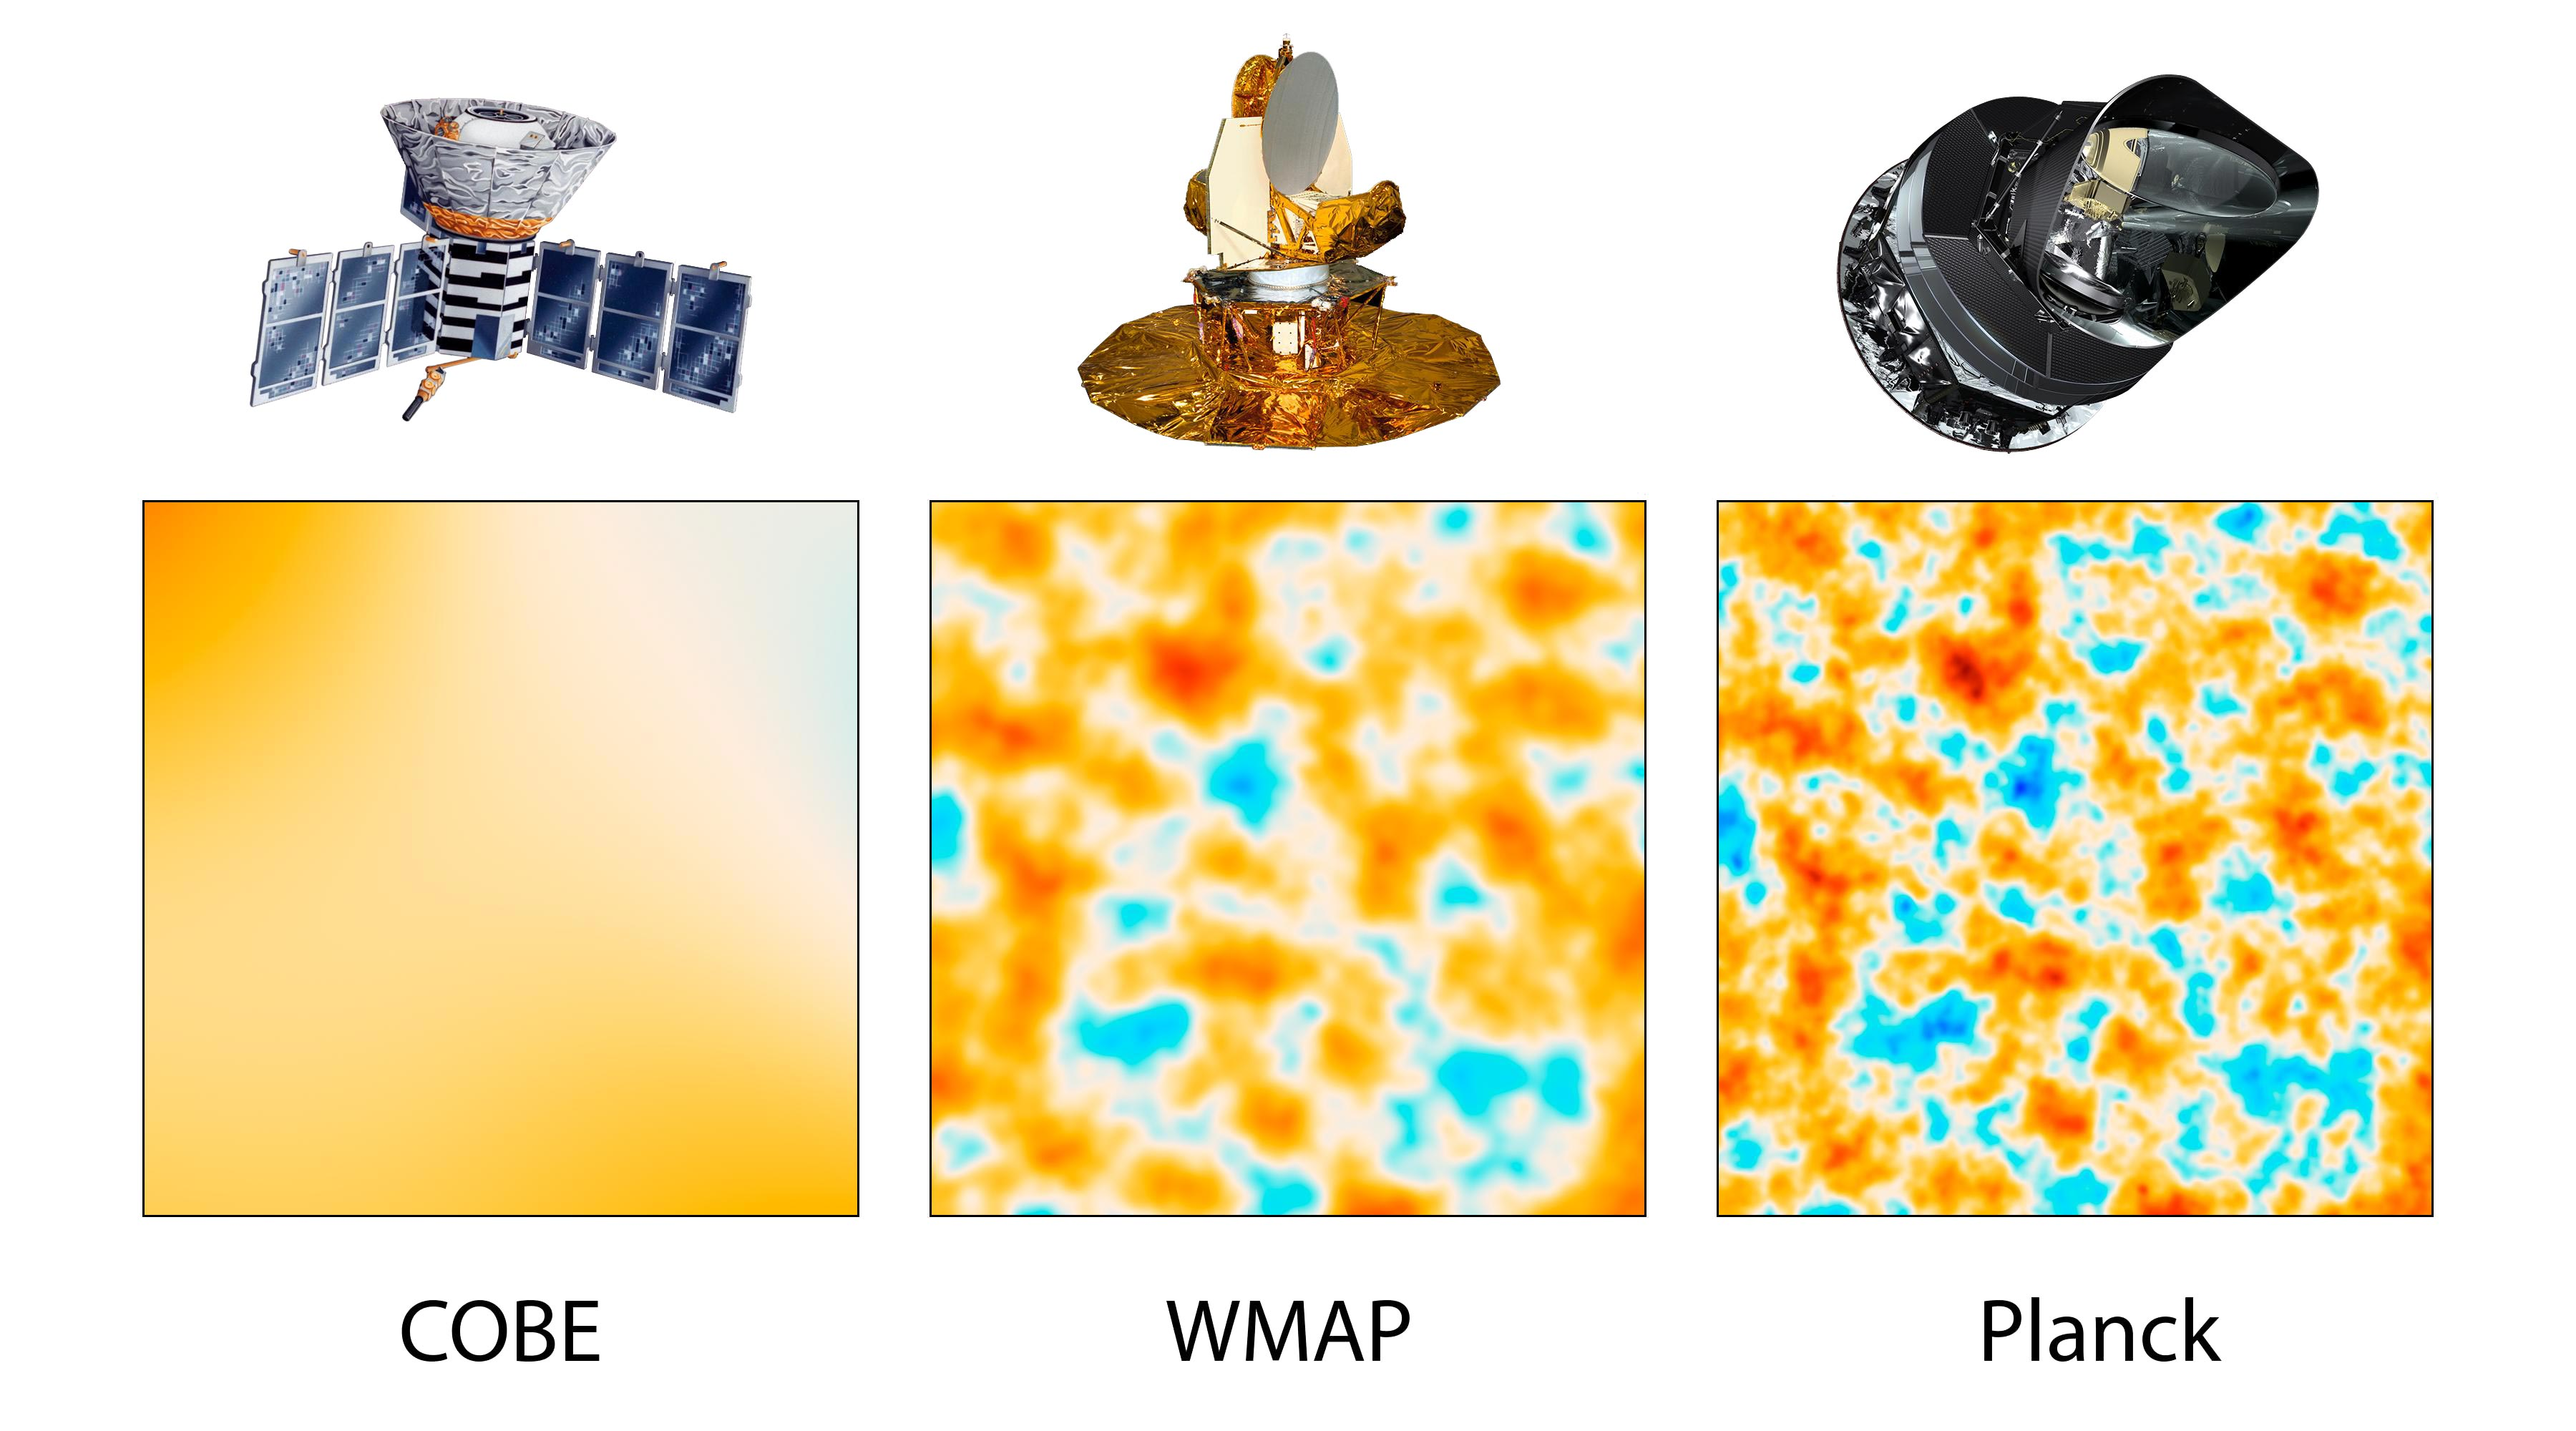
\includegraphics[width=\textwidth]{Intro-FIGS/planck_wmap_cobe.jpg}
\caption[A comparison between three generations of space CMB experiments. Image credit: NASA/JPL-Caltech/ESA.]{A comparison between the resolutions of COBE \citep{COBE}, WMAP \citep{WMAP_MapsResults}, and Planck \citep{planck2013} and the respective cosmic microwave background temperature maps. Panels show the same 10 deg$^2$ patch of the sky where the Planck resolution is around $5'$ whereas COBE's resolution is $7^o$ and WMAP's resolution is $20'$. Image credit: NASA/JPL-Caltech/ESA.}
\label{fig:PlanckWMAPCOBE}
\end{center}
\end{figure}
The Planck Satellite \citep{planck2013} is an European Space Agency telescope, situated at the L2 Lagrangian point of the Earth-Sun's system, aimed to make observations of the Cosmic Microwave Background, the first light of the Universe as it became transparent to electromagnetic radiation at the end of recombination era around 13.3 billion years ago. The Planck Satellite is a part of what is called a `Stage 3' CMB experiment and it took data between 2009 and 2013. Previous space-based CMB experiments are the Wilkinson Microwave Anisotropy Prope (WMAP, \citealt{WMAP_MapsResults}) working between 2001 and 2010, and the Cosmic Background Explorer (COBE, \citealt{COBE}) working between 1989 and 1993. Differently from its predecessors, the Planck Satellite contained very sensitive detectors, capable of measuring the polarisation of CMB photons with great accuracy and the temperature spectrum with impressive resolution. Figure \ref{fig:PlanckWMAPCOBE} shows a comparison between the three probes' resolutions in the same 10 deg$^2$ patch of the sky.


\qquad With impressively good resolution for temperature and polarisation measurements, having taken data in nine different frequencies, the Planck Collaboration released to date three cosmological parameter estimation results using temperature and polarisation auto- and cross-power spectrum, CMB lensing and low-mode polarisation \citep{planck2013,PlanckCosmology2016,2018PlanckCosmology}. The latest results were released in 2018 and are presented in \cite{2018PlanckCosmology} \footnote{The cosmological likelihood codes for the 2018 results are not available to date.} constituting one of the most precise and reliable cosmological measurements to date with percent level constraints in early Universe cosmological parameters like the primordial power spectrum amplitude, $A_s$; the scalar spectral index, $n_s$; the reionisation's optical depth, $\tau$. Details on how Planck's data are used in this work are presented in Section \ref{Sec:ExternalData}.

% \begin{itemize}
% \item outline the survey
% \item what Planck measures
% \item what is considered in this work about it
% \item temperature, polarisation, lensing
% \item description of their cosmological findings
% \end{itemize}

\subsection{Baryon Oscillation Spectroscopic Survey (BOSS)}
As a part of the Sloan Digital Sky Survey (SDSS) Phase-III, the Baryon Oscillation Spectroscopic Survey (BOSS, \citealt{BOSS}) is currently the largest galaxy redshift galaxy survey and it is the main dataset used in Chapters \ref{Chap:BOSS}, \ref{Chap:BOSS-Cosmo}, and \ref{Chap:Neutrinos}. The main purpose of BOSS is to perform a spectroscopic follow-up of SDSS photometric luminous red galaxies and quasars using a multiple-object spectrograph. The survey ran between 2008 and 2014 and obtained spectra for more than 1.5 million galaxies up to $z\approx 0.8$ \citep{BOSSCatalogue2016} and 160,000 quasars between $2.2 < z < 3$ using the Lyman-$\alpha$ spectra \citep{2013LyAlphaBOSS}.

\qquad The main objective of BOSS Collaboration was to measure and obtain cosmological parameters from the BAO scale across a variety of redshifts and methods\footnote{\cite{2017RossBOSS,2017BeutlerBOSS,2017Beutler2BOSS,2017SatpathyBOSS,2017SanchezBOSS,2017GriebBOSS,2017SalazarBOSSwTheta,2017WangBOSS,2017ZhaoBOSS}}. Using LRGs, the Collaboration obtained angular diameter distance and Hubble flow measurements with $\sim 2\%$ precision for intermediate redshifts, $0.3 < z < 0.55$, with a similar precision achieved using Ly-$\alpha$ quasars \citep{2013LyAlphaBOSS,2017QuasarsBOSS}. A compilation of BOSS Collaboration results for the galaxy sample can be found in \cite{2016BOSSCosmology} together with their consensus cosmological results for the last BOSS data release, DR12. A more detailed discussion of the BOSS LSS galaxy sample, including target selection criteria, angular selection functions, redshift distribution, and more can be found in Section \ref{Sec:Data}.

% \begin{itemize}
% \item SDSS-III description
% \item main goal and outline
% \item BOSS BAO description
% \item the consensus cosmology
% \end{itemize}

% \subsection{Dark Energy Survey}
% \RED{I don't actually use DES, do I?}
% \begin{itemize}
% \item DES description
% \item 3x2pts statistics analysis
% \item Talk about their Y1 results
% \end{itemize}

\subsection{Euclid Satellite}
The Euclid Satellite is an European Space Agency future mission which will perform 6 years long near-infrared and visual observations over 15,000 deg$^2$ for a wide angle survey, and a 40 deg$^2$ deep survey \citep{2011EuclidRedPaper}. The satellite will observe the sky in three different ways: photometric visible imaging in R+I+Z bands (550-900 nm) and near-infrared imaging in three different bands -- Y (920 - 1146 nm), J (1146 - 1372 nm), and H (1372 - 2000 nm), and a near-infrared slit-less spectroscopy (1100-2000 nm) over all the survey area. The visual imaging instrument has $0.1 ''$ resolution, while both the NIR instruments have an angular resolution of $0.3''$.

\qquad Euclid's primary science goal is to probe the expansion and structure formation history of the Universe up to redshift $z\sim 2$. Combining state-of-the-art imaging and slit-less spectroscopy makes Euclid the ultimate cross-correlations machine. Euclid will be able to combine large scale structure of galaxies, with outstanding photometric and spectroscopic redshift precision, $\sigma^{\text{photo}}_z/(1+z) < 0.05$ and  $\sigma^{\text{spec}}_z/(1+z)< 0.001$, respectively. Galaxy shape measurements for cosmic shear will have an equally impressive precision \citep{2016SartorisEuclid,2016SellentinWLEuclid}. Combining these probes in a concise framework is key to achieve the necessary precision to measure Euclid science goal's key cosmological parameters: the evolution of dark energy's equation-of-state, $w(z)$; the growth factor in a framework of modified gravity, $\gamma$; the sum of neutrino masses, $\sum m_{\nu}$, and their hierarchy; and the non-Gaussianity parameter, $f_{NL}$, related to inflationary models \citep{2011EuclidRedPaper}.

\subsection{Supernovae Type Ia Compilations}
\begin{figure}
\begin{center}
%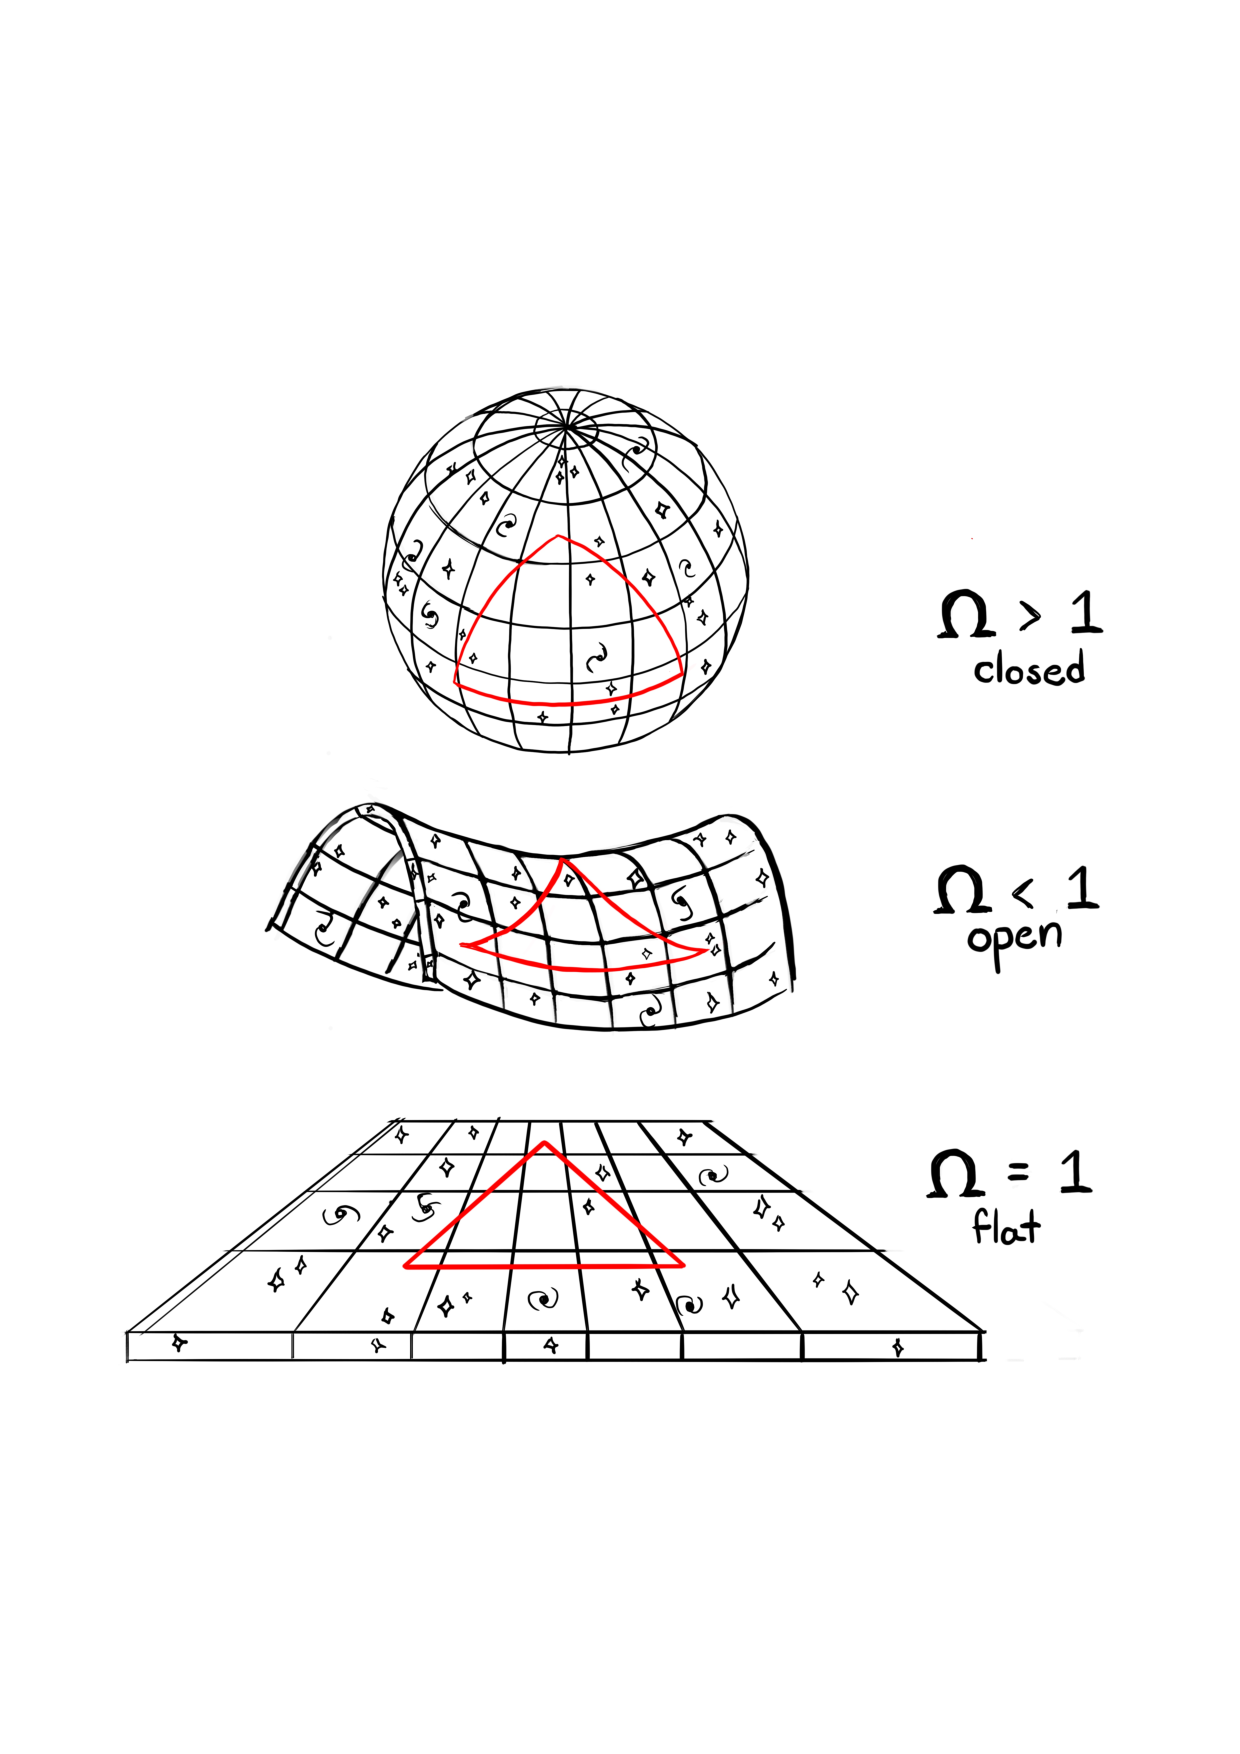
\includegraphics[width=\columnwidth]{Intro-FIGS/universeGeometry}
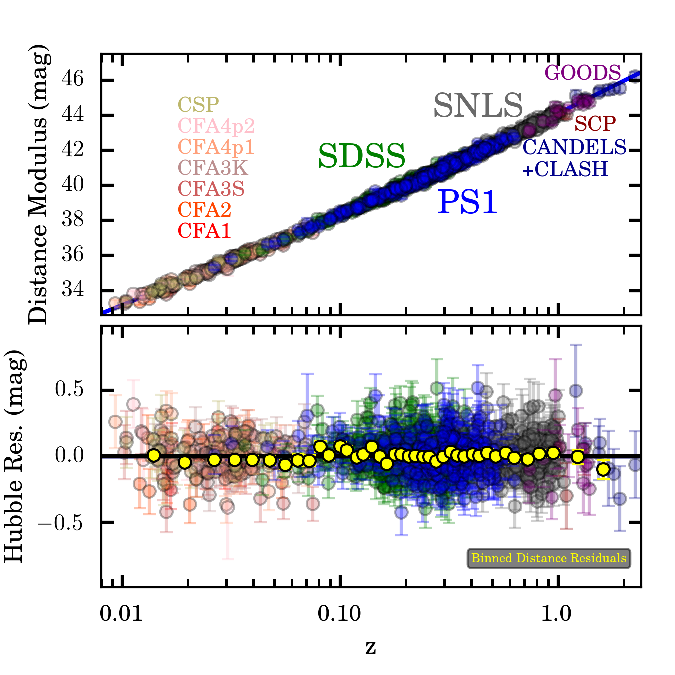
\includegraphics[width=\textwidth]{Intro-FIGS/hubble.pdf}
\caption[Hubble Diagram for the Pantheon Sample. Image credit: \cite{2018Pantheon}.]{Hubble Diagram for the Pantheon Sample. The \textit{top panel} shows the distance module as a function of redshift while the \textit{bottom panel} shows the residuals for the best-fit $\Lambda$CDM cosmology, $\Delta \mu \equiv \mu - \mu_{\text{best-fit}}$. Note that the Pantheon Sample contains the JLA sample as it can be seen as an updated version of it, including some new SNe Ia from the Pan-STARRS Survey \citep{2016-PanStarrs}. Image credit: \cite{2018Pantheon}.}
\label{fig:Pantheon}
\end{center}
\end{figure}
Supernovae Type Ia (SNe Ia) light-curve analysis compilation are crucial to cosmological data analysis; they were the first tools used to confirm that our Universe is going through a phase of accelerated expansion \citep{1998Riess,1999Perlmutter}. After being photometrically detected by differential imaging, spectroscopically confirmed SNe Ia have accurate redshift measurements and can be used as standardisable candles. This analysis is done via comparing the observed, $m_{\text{obs}}$, and the corrected magnitude, $M$, of a high redshift SNe Ia sample. One can then infer which set of cosmological parameters best-fits the so-called `distance modulus', defined as \citep{2007Salt-2,JLAdata}
\begin{equation}
    \mu = m_{\text{obs}}^* - (M_B + \alpha x_1 - \beta c)
\end{equation}
where $m_{\text{obs}}^*$ is, usually, the observed peak magnitude in the $B$-band; $x_1$ describes the time st reaching of the measured light-curve; $c$ is related to the individual supernovae colour at maximum brightness; the other parameters, $M_B, \alpha$, and $\beta$ are nuisance parameters. Some of these parameters, such as $M_B$ and $\beta$ are known to have a dependency on the host galaxy environment \citep{2011Sullivan}. The distance modulus can be compared with theoretical predictions using the following expression:
\begin{equation}
    \mu_{\text{th}}(z) = \lo(d_L(z)/10\, \text{pc})\, ,
\end{equation}
where the distance, $d_L$, is defined as 
\begin{equation}
    d_L(z) = \frac{1}{H_0}\lim_{\Omega_k' \rightarrow \Omega_k}\frac{(1+z)}{\sqrt{\Omega_k'}}\sinh\left( \sqrt{\Omega_k'}\int_0^z\frac{dz'}{E(z')}\right)
\end{equation}
with $E(z)$ defined as in Equation \eqref{Eq:Intro:HubbleOmega2}.

\qquad Throughout this work I make use of two Supernovae Type Ia (SNe Ia) light-curve analysis compilation. The first sample, used in Chapter \ref{Chap:BOSS-Cosmo}, is the Joint Light-curve Analysis (JLA) compilation \citep{JLAdata}; it contains spectroscopically confirmed SNe Ia from low redshift surveys, HST, SNLS \citep{2011Conley}, and SDSS-II \citep{2018Sako} -- with a total of 740 SNe Ia. The second sample, used in Chapter \ref{Chap:Neutrinos}, is the Pantheon compilation \citep{2018Pantheon}. It extends the JLA sample with the addition of spectroscopically confirmed SNe Ia from the Pan-STARRS Survey, with a total of 1048 SNe Ia with redshifts ranging from $0.01 < z < 2.3$. Details of the Hubble diagram for the Pantheon SNe Ia compilation and, consequently, from the JLA compilation can be found in Figure \ref{fig:Pantheon}.

\subsection{Big Bang Nucleosynthesis}
Big Bang Nucleosynthesis (BBN) is a very broad and extensive area of cosmology, here I present a brief review of the areas of this field relevant for the present work. A complete review on BBN can be found in \cite{2007Steingman-BBN} and, more recently, \cite{2016Particle-Review}.

\qquad Around the first twenty minutes of the Universe, the production of most of what it is considered to be `light elements' took place. These are $^3$He,$^4$He, D, and $^7$Li \citep{2007Steingman-BBN}. The abundances of such primordial elements provide us with information about the conditions of the Universe at very early stages, the very first minutes after what it is believed to be a `Big Bang'. At sufficiently high temperatures and densities for the primordial plasma, both protons and neutrons will fuse to form atomic nuclei. The main baryonic reactions at the very early Universe maintain chemical equilibrium, these are \citep[][p. 196]{2016Particle-Review,schneider_2016}:
\begin{align}
    p + e^- & \longleftrightarrow n + \nu \, , \label{Eq:proton1}\\
    p + \bar{\nu} & \longleftrightarrow n + e^+ \, ,\label{Eq:proton2}\\
    n & \rightarrow p + e^- + \bar{\nu}\, . \label{Eq:neutronDecay}
\end{align}

\qquad The reactions shown in Equations \eqref{Eq:proton1} and \eqref{Eq:proton2} are related to keeping the proton-to-neutron equilibrium ratio, while Equation \eqref{Eq:neutronDecay} is the free neutron decay with a time-scale of $\tau_n \approx 880$s. The ratio of the number of protons, $n_p$, to the number of neutrons, $n_n$, can be expressed via the Boltzmann factor in tems of the mass difference between the two particles, $\Delta m_{n,p} = m_n - m_p \approx 1.293$ MeV \citep{2015NeutronProtonRatio}:
\begin{equation}
    \frac{n_n}{n_p} = \exp\left[ - \frac{\Delta m_{n,p}}{k_b T}\right]\, .
    \label{Eq:BoltzFactorNeutronProton}
\end{equation}
As soon as the neutrinos freeze-out, this ratio is kept almost constant at $n_n/n_p \approx 1/3$. After this period of decoupling, this equilibrium between protons and neutrons is broken and no longer described by the Boltzmann factor in Equation \eqref{Eq:BoltzFactorNeutronProton}, the changes in this ratio are then governed to the decay of free neutrons on the above-mentioned time-scale, $\tau_n$. For neutrons to `survive' throughout the history of the Universe, these need to be found in the nuclei of atoms \citep{2007Steingman-BBN}.

\subsubsection{Deuterium and Helium abundances:}

\begin{figure}
\begin{center}
%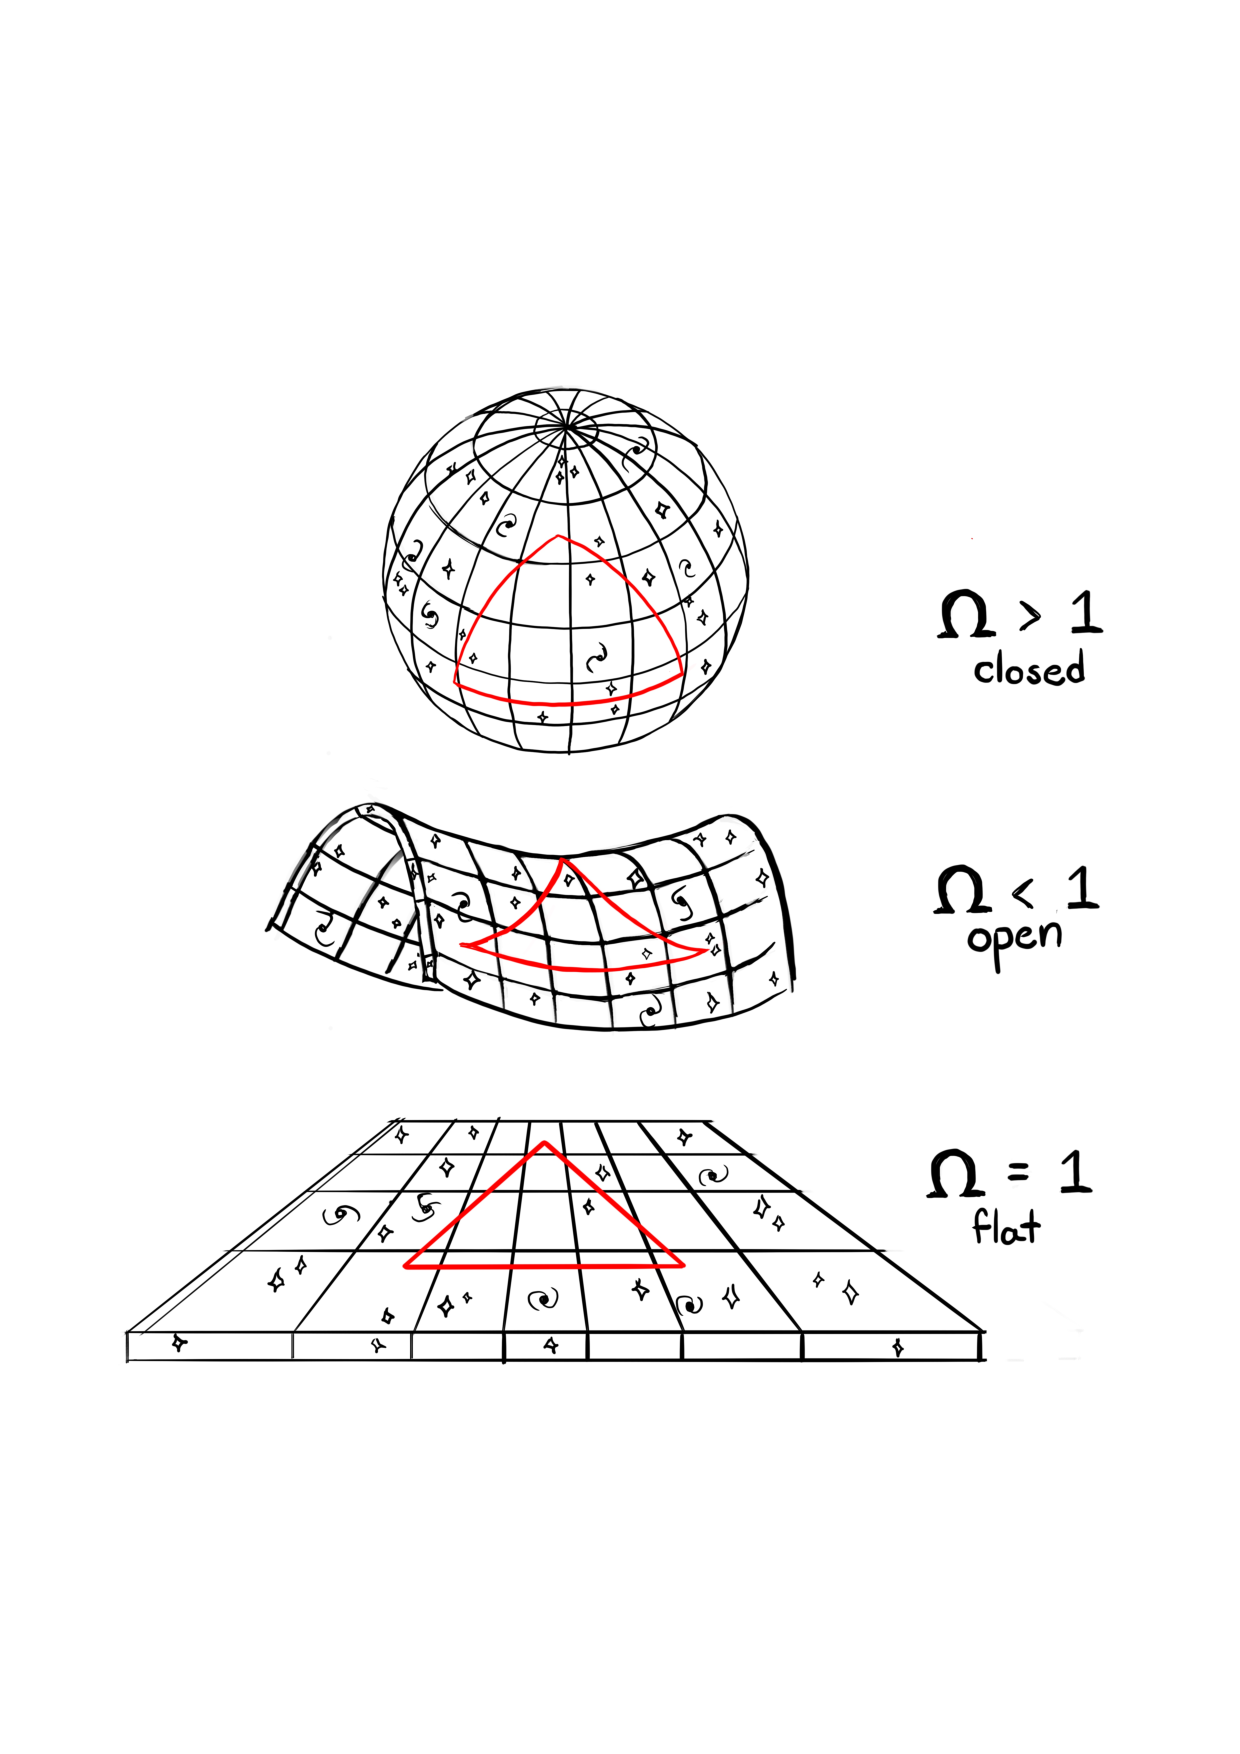
\includegraphics[width=\columnwidth]{Intro-FIGS/universeGeometry}
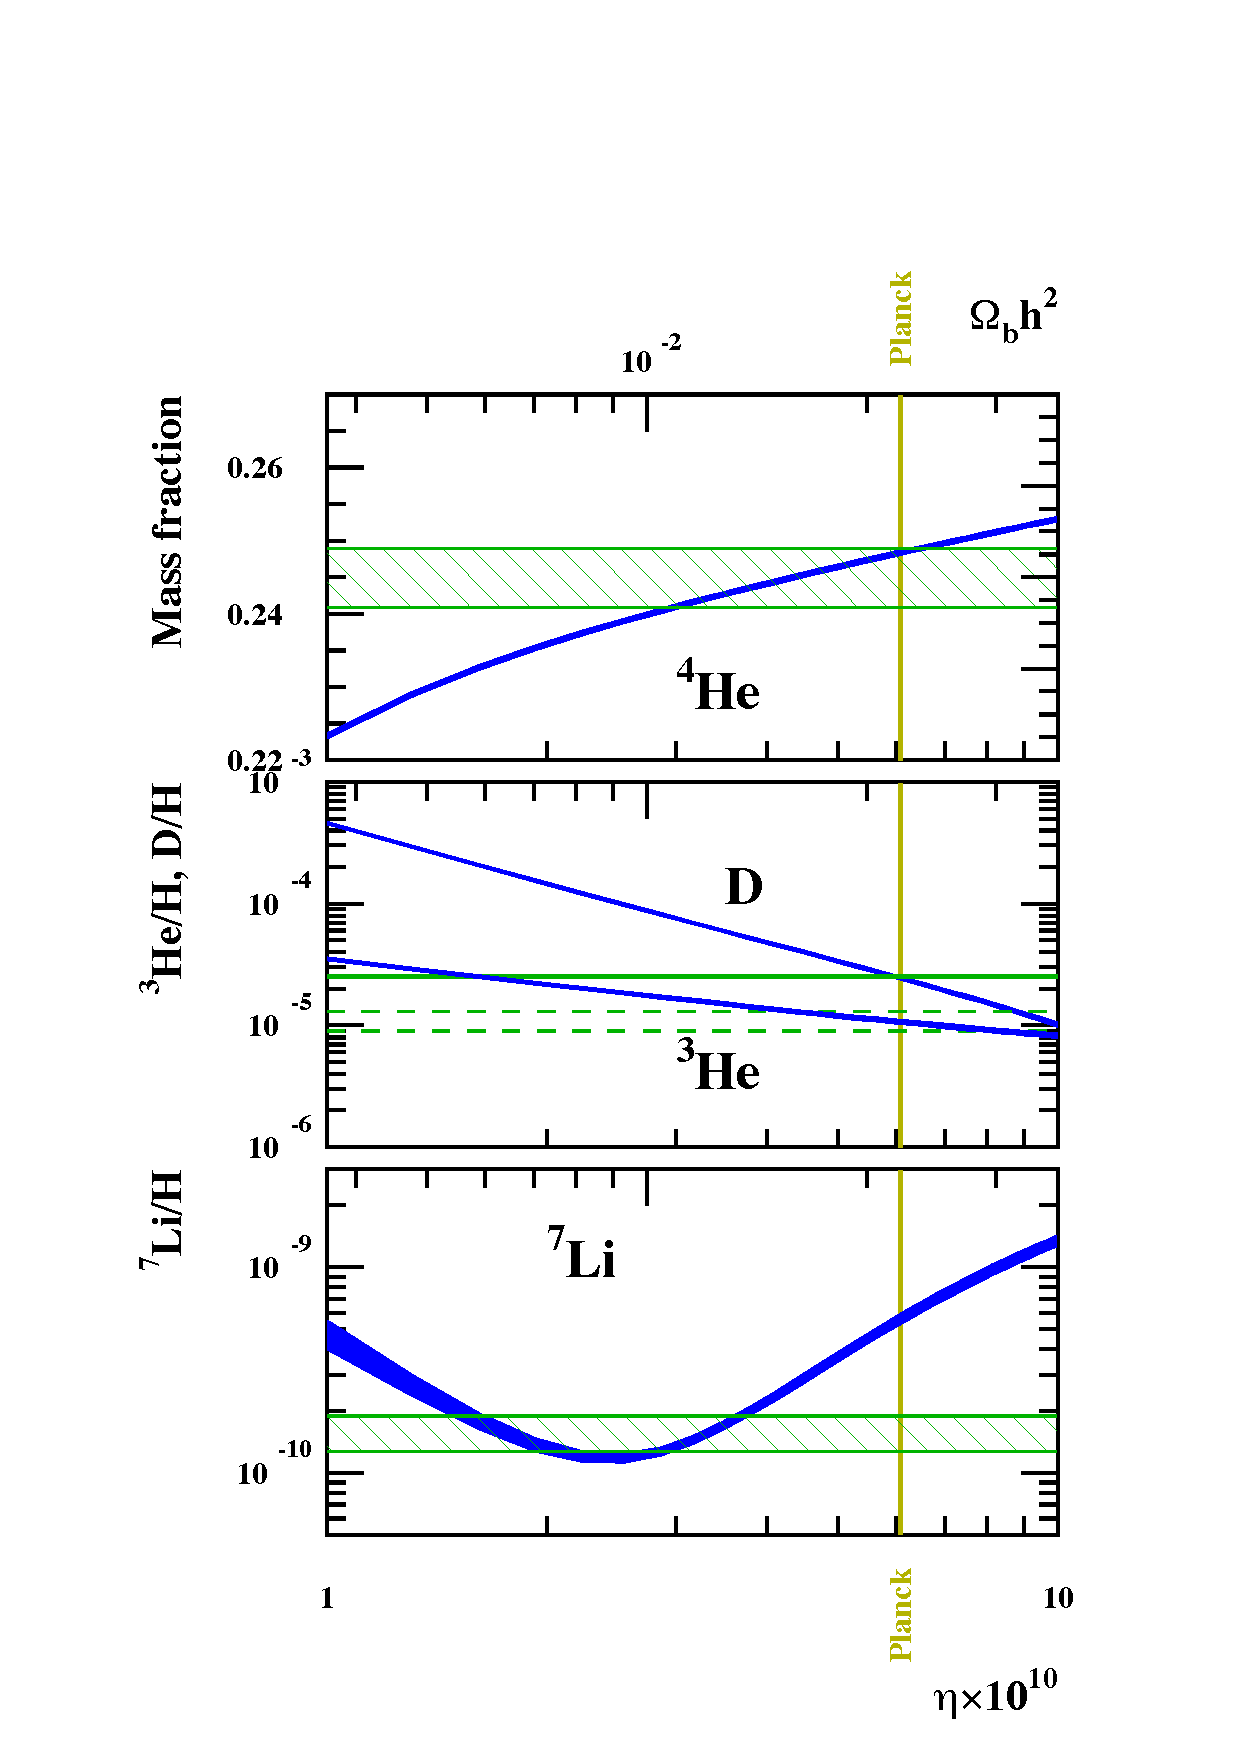
\includegraphics[width=\textwidth]{Intro-FIGS/heli2015.pdf}
\caption[BBN predictions for primordial abundances. Image Credit: \cite{2017-Abundances-Fig}]{BBN predictions for primordial abundances for $^4$He (mass fraction), D, $^3$He, and $^7$Li as a function of the baryon over photon ration, $\eta$, or the baryon density of the Universe, $\Omega_b h^2$. The vertical line comes from the Planck Collaboration measurements for $\Omega_b h^2$ presented in \cite{planck2013}; while the horizontal strips are from primordial abundances presented in \cite{2015-Abundances-Data}. Image Credit: \cite{2017-Abundances-Fig}.}
\label{fig:BBN}
\end{center}
\end{figure}

Deuterium is one of the simplest nucleus formed in the very early universe -- composed by a single proton and a single neutron, they are formed via the following reaction: $p + n \rightarrow D + \gamma$. As strong-force interactions govern the formation of deuterium, this is a very energy efficient reaction. Although, at the time of decoupling, since photons are much more abundant than baryons and the energy of some photons was much higher than the baryon's, $E_{\gamma} \geq E_{b}$, deuterium was destroyed by a mechanism called `photo-dissociation' \citep{2000Deuterium-Tyler}. Only when the temperature drops to around $T_D \approx 8\times 10^8$K that the deuterium formation rate wins over the dissociation rate, leading to a neutron-to-proton ratio of $n_n/n_p \approx 1/7$. Right after this period, all free neutrons end up firstly bound in deuterium atoms -- mostly due to the strong-force nature of the interactions.

\qquad With a higher binding energy than that of deuterium, $^4$He then starts forming as soon as the D density is sufficiently high. Having a higher binding energy ensures that helium-4 cannot be destroyed by photons via photo-dissociation. This process transforms almost all D into $^4$He, with the exception of a small fraction of deuterium. Since at this moment almost all neutrons are present in atoms of $^4$He, the number density of such nuclei can be estimated by taking into account the number of free protons after helium is formed: $n_{H} = n_p - n_n$. 

\qquad The `mass fraction Y` of $^4$He of the total baryon density is defined as \citep{2000-BBN-Review,2016R-BBN-Review}:
\begin{align}
    Y & = \frac{4n_{He}}{4n_{He}+n_H} \\
      & = \frac{2n_n}{n_p + n_n} \approx 0.25\, ,
\end{align}
given that the ratio $n_n/n_p \approx 1/7$ at the time deuterium formation ratio has enough temperature to win over photo-dissociation to form helium-4. This result means that at least a quarter of the Universe's baryonic content should be in the form of helium-4 and it is with perfect agreement with observations \citep{2015-Abundances-Data,2017-Abundances-Fig}.

\qquad From Figure \ref{fig:BBN}, one can see that there's a strong dependency between the $^4$He and D abundances and the baryon content of the Universe, $\Omega_b$. With a larger baryon density, two main consequences arise for these two abundances. The first one is that, with a larger baryon-to-photon ratio, deuterium would form much earlier, with fewer neutrons decaying leading to a higher value for Y. The second consequence, in a similar reasoning, would be that deuterium would convert into helium-4 much more efficiently, leading to a much lower fraction of D.

\qquad Lastly, neutrinos play a major role in BBN given the epoch of the 
Universe one considers. At such early times, neutrinos act as relativistic which influence BBN in various ways. As an example, electron neutrinos influence and control the fraction of free neutrons available, limiting the formation of primordial $^4$He. The number of active neutrinos, $N_{\nu}$, also change considerably predictions for BBN abundances. If $N_{\nu} > 3$, fewer neutrons would decay, resulting in a much higher helium-4 abundance \citep{2007Steingman-BBN,schneider_2016}.


% \begin{itemize}
% \item characteristics of the Euclid mission
% \item Description of euclid's observational strategy 
% \item Euclid's Impact in the future of cosmology
% \item Euclid as a cross-correlation's machine
% \end{itemize}

%%%%%%%%%%%%%%%%%%%%%%%%%%%%%%%%%%%%%%%%%%%%%%%%%%%%%%%%%%%
%   				THESIS STRUCTURE
%%%%%%%%%%%%%%%%%%%%%%%%%%%%%%%%%%%%%%%%%%%%%%%%%%%%%%%%%%%
\section{Thesis Structure}
\label{sec:intro:structure}
At last, I outline here the structure of chapters to come together with the list of authors and collaborators in the published and to be published papers related to the work presented in each chapter.

\textbf{Chapter \ref{Chap:BOSS}}: \textit{Tomographic Analysis of BOSS DR12 Galaxy Clustering in Harmonic Space} \\[0.6em]
In this following chapter, I present the work I have done performing an angular power spectrum analysis of BOSS Large Scale Structure galaxy catalogue from \cite{BOSSCatalogue2016}. In this work, I depart from the official LSS BOSS catalogues and masks. I then proceed to build up the full schema in order to extract cosmological information using a harmonic decomposition framework: galaxy maps and masks, angular power spectra measurements with a Pseudo-$C_{\ell}$ estimator, the theoretical $C_{\ell}$ formalism, and construction and validation of a covariance matrix. Finally, in order to assess the viability of using the full shape of the angular power spectra for a cosmological analysis, I have performed systematic contamination null-tests to ensure the measured $C_{\ell}$s were clean from any sort of photometric and observational effects.

\qquad This work, presented in \cite{2018LoureiroBOSS}, has been accepted for publication by Monthly Notices of the Royal Astronomical Society (MNRAS) and it was performed in collaboration with Bruno Moraes, Andrei Cuceu, Michael McLeod, Lorne Whiteway, Sreekumar T. Balan, Aur\'elien Benoit-L\'evy, Ofer Lahav, Marc Manera, Richard Rollins, and Henrique S. Xavier.

\bigskip

\textbf{Chapter \ref{Chap:BOSS-Cosmo}}: \textit{Cosmological Measurements from Angular Power Spectra Analysis of BOSS DR12 Tomography} \\[0.6em]
 In this Chapter, I outline the procedures and formalism to perform a Bayesian analysis for cosmological inference using measurements of the angular power spectra. I then proceed to perform high level consistency checks on the angular power spectra measurements produced in Chapter \ref{Chap:BOSS}, as well as consistency checks on the cosmological inference pipeline and the covariance matrices produced for and with the BOSS-$C_{\ell}$s. Finally, when combining this new BOSS data vectors with CMB data from the Planck experiment and the JLA SNe Ia compilation data-set, I demonstrate that extremely competitive cosmological constraints can be obtained from a large scale structure analysis of spectroscopic galaxies in harmonic space. 

\qquad This work, also presented in \cite{2018LoureiroBOSS}, has been accepted by Monthly Notices of the Royal Astronomical Society (MNRAS) and it was performed in collaboration with Bruno Moraes, Andrei Cuceu, Michael McLeod, Lorne Whiteway, Sreekumar T. Balan, Aur\'elien Benoit-L\'evy, Ofer Lahav, Marc Manera, Richard Rollins, and Henrique S. Xavier.

\bigskip

\textbf{Chapter \ref{Chap:Neutrinos}}: \textit{Neutrino Masses from Combined Cosmological Probes and Oscillation Experiments' Constraints} \\[0.6em]
In this follow-up chapter, I investigate the impact of several neutrino mass models in the determination of the upper bound of the sum of neutrino masses, $\sum m_{\nu}$. I demonstrate that a physically motivated model, which takes into account constraints from particle physics experiments, can not only yield robust constraints on \NM{} when compared to usual cosmological approximation, but also to set an upper bound to the mass of the lightest neutrino mass species. This analysis was performed using the BOSS data vector in harmonic space in combination with Planck CMB and Lensing, SNe Ia from the Pantheon compilation, and BBN data from deuterium-to-hydrogen fraction.

\qquad This work, presented in \cite{2018LoureiroNeutrinos}, has been submitted to Physical Review Letters (PRL) and it was performed in collaboration with  Andrei Cuceu, Bruno Moraes, Lorne Whiteway, Michael McLeod, Sreekumar T. Balan, Aur\'elien Benoit-L\'evy, Ofer Lahav, Marc Manera, Richard Rollins, and Henrique S. Xavier.

\bigskip

\textbf{Chapter \ref{Chap:BPL}}: \textit{An investigation of Bayesian Angular Power Spectra Estimators applied to Galaxy Clustering} \\[0.6em]
The main goal of this chapter was to extend, test, and benchmark a general Bayesian angular power spectra estimator for data distributed on a sphere with a final goal of being a part of the official Euclid $C_{\ell}$ estimator pipelines. The method was originally developed to be applied to CMB temperature, CMB polarisation modes by \cite{SreeThesis}. In this chapter I perform the necessary adaptations to investigate an application of the method to galaxy clustering -- with a future goal to extend it to weak lensing convergence ($\kappa$), cosmic shear ($\gamma_1$ \& $\gamma_2$), and cross-correlations of all previous probes. I perform a series of tests related to the impact of the survey's geometry in the spherical harmonics and its impact in the estimated angular power spectra of galaxies. Finally, I produce and test the method in Euclid-like log-normal simulations for two contrasting noise scenarios, demonstrating that the ideal way to deal with the noise in the case of galaxy clustering is to treat it as anisotropic.

\qquad This is an investigatory chapter with preliminary results. Extending this work to the point of completion is one of the objetives on my work as an Euclid Research Assistance in the next year. This work is in preliminary preparation to be submitted to MNRAS and it was performed in collaboration with Sreekumar T. Balan, Lorne Whiteway, Andrei Cuceu, Lee Whittaker, and Malak Olamaie.

\bigskip

\textbf{Chapter \ref{Chap:Conclusions}}: \textit{Final Considerations, Conclusions \& Future Prospects} \\[0.6em]
I finalise this work by highlighting some key points learned from performing this extensive analysis of the BOSS data release 12 spectroscopic data-set and the resulting cosmological findings. Here I point out my contributions to the narrow field of using spherical harmonics to study and understand the large scale structure of galaxies in the Universe and its cosmological implications not only for cosmology but also for neutrino physics. Moving on, I comment on future prospects of my work, natural extensions of it, and a 5 year broad plan for future research and contributions.

% \textbf{Chapter \ref{sec:conclusion}} \\[0.2em]
% \blindtext
 % INCLUDE: introduction
% !TEX root = ../thesis-example.tex
%
%\chapter{Cosmological Measurements from Angular Power Spectra analysis of BOSS DR12 Tomography}
\chapter{Tomographic Analysis of BOSS DR12 Galaxy Clustering in Harmonic Space}
\label{Chap:BOSS}

\cleanchapterquote{If you’re going to try,\\
go all the way.\\
There is no other feeling like \\
that. \\
You will be alone with the gods \\
and the nights will flame with \\ 
fire.}{Charles Bukowski}{(Roll the Dice)}
\vspace*{\fill}

In this chapter, I perform an angular power spectra analysis of the Baryon Oscillation Spectroscopic Survey DR12 galaxies, a spectroscopic follow-up of around 1.3 million SDSS galaxies over 9,376 deg$^2$ with an effective volume of $\sim 6.5$ (Gpc $h^{-1}$)$^3$ in the redshift range $0.15 \leq  z  < 0.80$. I split this sample into 13 tomographic bins ($\Delta z = 0.05$); angular power spectra were calculated using a Pseudo-$C_{\ell}$ estimator. Measurements were then binned with a bandwidth of $\Delta \ell = 8$. Covariance matrices were estimated using log-normal simulated galaxy maps using the measured angular power spectra instead of a fiducial $C_{\ell}$. These were validated using a Gaussian expression for the variance of the Pseudo-$C_{\ell}$ estimator which takes into account effects introduced by the partial sky nature of the observations -- the mixing of modes due to the mask. Finally, in order to use the full shape of the angular power spectra for Cosmological analyses, I have performed null-tests of systematic contamination against eighteen different sources of systematics by using cross-correlations between the data and systematics. Apart from the larger modes -- the first bandwidth $\ell$-modes -- I have found no significant contamination from observational systematics, indicating that the full shape of BOSS DR12 angular power spectra of galaxies can be used for cosmological analysis.

\textit{The work presented in this chapter was presented in \citet{2018LoureiroBOSS}.} 

\newpage
%%%%%%%%%%%%%%%%%%%%%%%%%%%%%%%%%%%%%%%%%%%%%%%%%%%%%%%%%%%%%%%%%%%%%%%%
% 					   % INTRODUCTION %
%%%%%%%%%%%%%%%%%%%%%%%%%%%%%%%%%%%%%%%%%%%%%%%%%%%%%%%%%%%%%%%%%%%%%%%%
\section{Introduction}\label{sec:BOSS:intro}
Recent years have seen increased interest in measuring cross-correlations of distinct cosmological probes. Simultaneously modelling and fitting auto- and cross-correlations of observable cosmological fields can improve the dark energy figure-of-merit of surveys \citep{2008PhRvD..77l3525W}, provide better control of systematic errors, and potentially unveil new physics \citep[e.g.][]{Kirk2015}. Examples of this approach include combinations of CMB primary and secondary anisotropies with galaxy clustering and cosmic shear signals that help to constrain galaxy bias and intrinsic alignments \citep{Giannantonio2016, Hand2015}, `3x2pt' correlations between galaxy clustering and lensing signals which provide the strongest low-redshift constraints on cosmological models \citep{2017MNRAS.465.1454H, 2017arXiv170801530D}, and also between galaxy clustering and CMB \citep{2016Nicola, 2017Nicola, Doux2017}.

\qquad A consistent treatment of all probes requires a common theoretical framework for the analysis of the data and covariance matrices across the different correlations. A natural candidate for this is the angular power spectrum. It has been in widespread use by the CMB community for decades \citep{COBE,Healpix,Polspice0,PolSpiceSzapudi2001,PolSpice2001}, providing several advantages over other statistical estimators. Spherical harmonic decompositions are particularly suited to the analysis of data on the sphere, as they are easily connected to the underlying linear cosmological perturbations in a statistically isotropic and homogeneous Universe, and possess a simple covariance structure for most practical cases despite mode mixing from partial sky observations. Construction of the estimator from galaxy survey data does not require any de-projection using cosmological information, and covariance estimation from log-normal simulations can be estimated in a cosmology-independent way. This allows for a consistent end-to-end analysis. Last, but not least, self-calibration of photometric redshift distributions using cross-correlations with spectroscopic surveys is more readily implemented, and more robust to potential systematic errors \citep{McQuinnWhite2013, 2016McLeod} when compared to other methods such as $P(k)$, $\xi(r)$ and $w(\theta)$ \citep{2017RossBOSS,2017SalazarBOSSwTheta}.  In this chapter, it is argued that this should be the case because methods which live in angular space such as the method presented here and $w(\theta)$ can be naturally binned finely and hence more information about the redshift evolution can be extracted without further modelling and further assumptions. It is also further argued that non-linearities are better separated in this method that they would be if using the data in configuration space.

\qquad Spectroscopic surveys give precise information about the radial distances to galaxies, since the redshifts can be precisely measured from the spectra. In light of the precision in redshift for such galaxy surveys, the usual cosmological approach is the use the 3D power spectrum, $P(k)$, or the 3D correlation function in real space, $\xi(r)$ \citep{2001Percival,2017RossBOSS,2017BeutlerBOSS,2017WangBOSS}. Although these approaches have some advantages related to exploring the full radial information from spectroscopic surveys, a fiducial cosmology always needs to be assumed in order to translate from redshift space to real space. This choice of fiducial cosmology may potentially bias cosmological measurements, justifying once more the choice of a tomographic angular power spectra analysis.

\qquad However, there are difficulties involved in using angular power spectrum estimators on a spectroscopic galaxy survey. Firstly, it is not simple to ensure that all of this radial information is contained in the angular power spectra of projected redshift bins - even if a fine redshift binning strategy is employed. A second and more relevant issue is that spectroscopic surveys have a much lower galaxy density due to necessarily long integration times and targeting of specific galaxies with fibre spectrographs. This leads to a low signal-to-noise ratio of galaxies to Poisson noise once the data are projected in several tomographic redshift bins. A judicious choice of redshift bin width and Fourier scales can ensure that all relevant linear cosmological information is retrieved \citep{Asorey2012, Gaztanaga2012, Eriksen2015, Kirk2015}, but no consistent application of 2D angular power spectra tomography with multiple narrow bins has been attempted on real spectroscopic survey data.\footnote{However, \citet{2017SalazarBOSSwTheta} perform a similar analysis in real space with the BOSS DR12 galaxies.}

\qquad In this work, I apply the angular power spectrum formalism to the Baryon Oscillation Spectroscopic Survey 12th and final public data release (BOSS DR12). The Baryon Oscillation Spectroscopic Survey (BOSS) is one of the components of the third phase of the Sloan Digital Sky Survey (SDSS-III). Its main aim is to measure the preferred scale of baryonic acoustic oscillations in the primordial baryon-photon plasma, as imprinted in the late-time galaxy distribution. The DR12 data release contains the largest spectroscopic catalogue to date \citep{BOSS2015}. It is based on observations of around 2.5 million objects of which around 1.5 million were classified as galaxies, which are further selected to form a large-scale structure galaxy sample ready for cosmological analysis \citep{BOSSCatalogue2016}. I decided to work with this data set because of its constraining power, its public availability, and because of the possibility of comparing my results to those previously obtained by the BOSS collaboration with this same data set (see \citealt{2016BOSSCosmology} and the BOSS publications website\footnote{http://www.sdss3.org/science/boss\underline{~~}publications.php} for a list of cosmological publications from the collaboration).

\qquad Using the BOSS large-scale structure sample, I show that it is possible not only to measure the full shape of the angular power spectra in very thin tomographic redshift bins, but also to obtain reliable cosmological constraints for $\Lambda$CDM, $w$CDM and $\Lambda$CDM with $\sum m_{\nu}$ cosmologies using such a survey alone (See Chapter \ref{Chap:BOSS-Cosmo}). The method presented here uses the full shape of the angular power spectra -- not just the BAO scale. This is achieved by separating the galaxy samples into tomographic redshift bins with $\Delta z = 0.05$, and using both the auto power spectra and the cross power spectra of adjacent bins to extract information from the radial correlation of galaxies.% Further combination with external CMB \citep{PlanckCosmology2016} and SNIa \citep{JLAdata} data sets achieves competitive constraints on the models mentioned above.

\qquad This chapter is organised as follows: Section \ref{Sec:Data} describes the BOSS LSS sample selection criteria, the mask creation, and the construction of the galaxy overdensity maps. Section \ref{Sec:Measurements} describes the Pseudo-$C_{\ell}$ estimator used for the angular power spectrum analysis. Section \ref{Sec:Theory} describes the theoretical modelling of the angular power spectrum and the use of log-normal mocks for covariance matrix estimation. Section \ref{Sec:Systm} describes the analysis of potential systematic errors using the cross-power spectra between the data and different sources of systematic effects. Finally, Section \ref{Sec:Concl1} concludes this Chapter by outlining the next steps towards probing cosmological parameters with the data-vector generated in this Chapter and used on the following Chapters. %Section \ref{Sec:CosmoBananas} explains the Bayesian modelling for cosmological parameter estimation, describes a series of consistency checks performed on the data, the covariance matrix, and the pipelines, and finally presents cosmological parameter constraints for flat $\Lambda$CDM, $w$CDM, and $\Lambda$CDM + $\sum m_{\nu}$ models using the BOSS $C_{\ell}$s alone and in combination with external CMB results from the Planck collaboration \citep{PlanckLikelihood2015} and type Ia supernovae results from JLA \citep{JLAdata}.

%%%%%%%%%%%%%%%%%%%%%%%%%%%%%%%%%%%%%%%%%%%%%%%%%%%%%%%%%%%%%%%%%%%%%%%%
% 					   			% DATA %
%%%%%%%%%%%%%%%%%%%%%%%%%%%%%%%%%%%%%%%%%%%%%%%%%%%%%%%%%%%%%%%%%%%%%%%%
\section{BOSS DR12 Data}\label{Sec:Data}
The Baryon Oscillation Spectroscopic Survey Data Release 12 (BOSS DR12) is one of the experiments from the third phase of the Sloan Digital Sky Survey (SDSS-III), providing the largest galaxy redshift survey to date. The full description of the BOSS DR12, including target selection criteria and systematics, can be found in \cite{BOSS2015}. 

\qquad The BOSS DR12 is subdivided into two main samples: LOWZ and CMASS. The BOSS Collaboration created these samples by applying colour-magnitude and colour-colour cuts to the SDSS photometric catalogue in order to generate lists of targets for spectroscopic observation. The LOWZ sub-sample is designed as a simple extension of the original SDSS Luminous Red Galaxy (LRG) sample \citep{2001Eisenstein} at low redshifts, while the CMASS  sample is defined to select a stellar mass-limited sample of galaxies of all colours - hence its name, for ``constant stellar mass" - complemented by a colour cut whose goal is to select higher-redshift objects. The targets were then observed spectroscopically and objects that revealed themselves not to be galaxies (e.g. stars or quasars) were discarded. For a comprehensive discussion of the photometric cuts, selection criteria, and the terminology used, see \cite{BOSS}.

\subsection{Galaxy Catalogues}
%\begin{wrapfigure}{r}{0.5\textwidth}
  \begin{figure}
  \vspace{-30pt}
  \begin{center}
      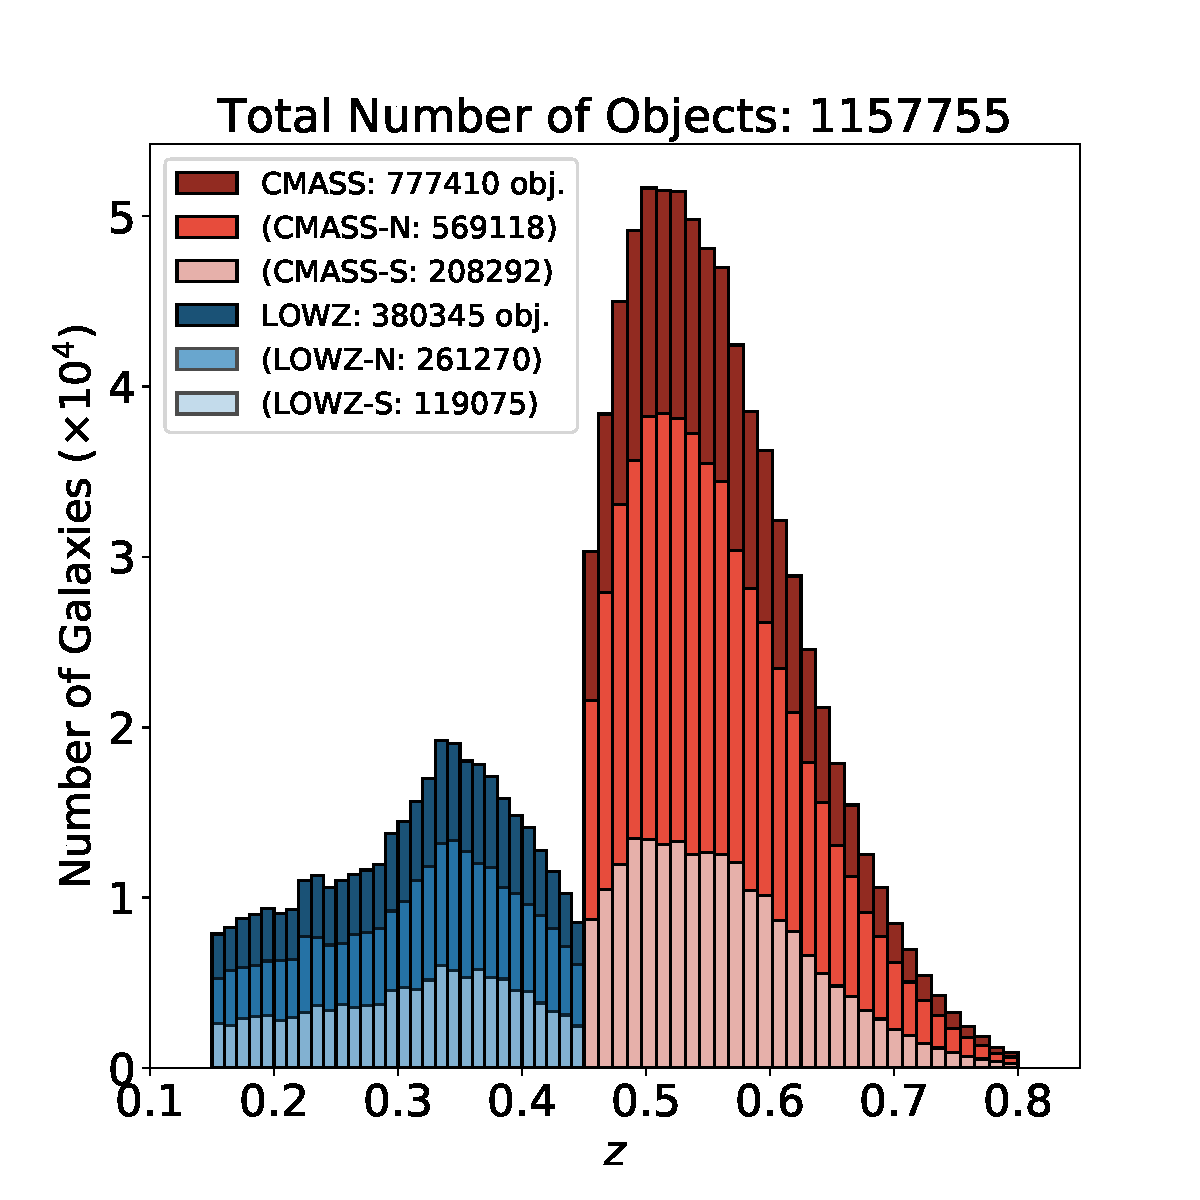
\includegraphics[scale=0.450]{BOSS-FIGS/Nz_BOSS}
      \caption[The redshift distribution of the different BOSS samples.]{The redshift distribution of the different BOSS samples. The darker histogram correspond to the total samples for LOWZ ($0.15\leq z <0.45$) and CMASS ($0.45\leq z < 0.80$). The overlap between samples was excluded using object ID, leaving a total number of 1,157,755 galaxies. Figure \ref{fig:Masks} shows the angular selection function for the samples.}
      \label{fig:NZ_BOSS}
      \end{center}
  \end{figure}
%\end{wrapfigure}
%In order to compare methods and results with the official BOSS collaboration results \citep{2016BOSSCosmology}, the construction of the catalogues in this work follows a similar procedure outlined in \cite{BOSSCatalogue2016} and the data was downloaded from the BOSS DR12 website\footnote{http://data.sdss3.org/sas/dr12/boss/}. This section outlines the main characteristics of the samples and a few differences in catalogue design tailored to the method I am using. Further details on the photometric cuts, selection criteria, and the terminology used can be found on the papers mentioned above\footnote{As mentioned, the main catalogue creation algorithm follows the algorithm outlined in \cite{BOSSCatalogue2016} and was not created by me nor any of my collaborators from Loureiro et al, \textit{in prep}.}.
To facilitate comparison of my results with the official BOSS collaboration results \citep{2016BOSSCosmology}, the construction of the catalogues used in this work followed a procedure similar to that outlined in \cite{BOSSCatalogue2016}. The data set was downloaded from the BOSS DR12 website.\footnote{http://data.sdss3.org/sas/dr12/boss/} I have further restricted these samples by applying redshift cuts of $0.15 \leq z < 0.45$ for LOWZ and $0.45 \leq z < 0.80$ for CMASS. These cuts ensure that the LOWZ and CMASS samples do not overlap in redshift, which simplifies the tomographic analysis. I use $z = 0.45$ (and not a lower $z$) as the dividing point between the two samples because the LOWZ sample has around $12\%$ more galaxies in $0.4 < z < 0.45$ than does CMASS. See figure \ref{fig:NZ_BOSS} for the resulting redshift distributions. Note also that the upper limit of $z < 0.8$ for CMASS is greater than the $z < 0.75$ limit used in \cite{BOSSCatalogue2016}. As a result of these factors the redshift ranges used in this work differ from those quoted in \cite{BOSSCatalogue2016} and \cite{2016BOSSCosmology}. Further details on the photometric cuts, selection criteria, and the terminology used can be found on the papers mentioned above\footnote{As mentioned, the main catalogue creation algorithm follows the algorithm outlined in \cite{BOSSCatalogue2016} and was not created by me nor any of my collaborators from \cite{2018LoureiroBOSS}.}. The subsections that follow outline the main characteristics of the samples.

\subsubsection{LOWZ Sample:}
The LOWZ sample is designed to contain luminous red galaxies (LRGs) with redshift up to $0.45$ as a extension of the SDSS-I/II LRG Cut I sample \citep{2001Eisenstein}. The targets are selected at low redshifts by a cut around the predicted colour locus (Equation \ref{Eq:ColourCutLZ}), and a selection of bright red objects is done at each redshift by a variable colour-magnitude cut in the \textit{r}-band (Equation \ref{Eq:RedSelecLZ}). This is the main cut in the LOWZ sample as it produces a constant number density on the redshift range of this sample. According to \cite{BOSSCatalogue2016}, the number of galaxies in the sample is extremely sensitive to this cut (see also \cite{2013ROSS}). Star-galaxy separation is done, for LRGs, with a cut on the \textit{r}-band magnitudes as shown in Equation \eqref{Eq:StarGalLZ}. Finally, to guarantee a high spectroscopic redshift success rate, a cut is performed on the \textit{r}-band to impose a brightness limit, as shown in Equation \eqref{Eq:FinalCutLZ}.

\qquad In summary, the photometric target selection criteria for the LOWZ sample is \citep{BOSSCatalogue2016}:
\begin{align}
 & |c_{\perp}| < 0.2 \label{Eq:ColourCutLZ} \\
 & r_{cmod} < 13.5 + c_{\parallel}/0.3 \label{Eq:RedSelecLZ} \\
 & r_{psf} - r_{cmod} > 0.3 \label{Eq:StarGalLZ} \\
 & 16 < r_{cmod} < 19.6 \label{Eq:FinalCutLZ}
\end{align}

\qquad In the first months of observation, the BOSS collaboration used a different star-galaxy separation criterion compared to that used later (see Appendix A from \citealt{BOSSCatalogue2016}). As a result, some sky regions from the LOWZ sample (specifically LOWZE2 and LOWZE3) have a redshift distribution that differs to that in other regions. As the method I am using relies on having a consistent redshift distribution across the sky, I excluded these regions from the LOWZ sample (see Figure \ref{fig:Masks}). 

\subsubsection{CMASS Sample:}
The CMASS sample was designed to be closer to a mass limited sample, extending the Cut-II LRGs from SDSS-I/II \citep{2001Eisenstein} to bluer and fainter objects using a sliding colour-magnitude cut as shown in Equation \eqref{Eq:CMCut2}. The cut in the quantity $d_{\perp}$ (Equation \ref{Eq:RedCutCM}) results in an increase in the number density of objects for the redshift range of $0.45 < z < 0.80$ (see Figure \ref{fig:NZ_BOSS}). Model and magnitude limit cuts (Equations \ref{Eq:CMCut3} and \ref{Eq:CMCut4}) ensure high redshift success rates while preventing low redshift objects from being erroneously targeted. Outliers and problematic blended objects are excluded using cuts in \textit{i}- and \textit{r}-band magnitudes (Equations \ref{Eq:CMCut5} and \ref{Eq:CMCutPix}). Finally, star-galaxy separation was done by performing a varying cut in $i_{psf} - i_{mod}$ and $z_{psf} - z_{mod}$ based on \cite{2006Cannon2Slaq} (Equations \ref{Eq:CMStarGal1} and \ref{Eq:CMStarGal2}).

\qquad In summary, the CMASS sample photometric target selection is \citep{BOSSCatalogue2016}:
\begin{align}
& i_{mod} < \min (19.86 + 1.6(d_{\perp}-0.8),19.9) \label{Eq:CMCut2} \\
& d_{\perp} > 0.55 \label{Eq:RedCutCM} \\
& 17.5 < i_{cmod} < 19.9 \label{Eq:CMCut3} \\
& i_{fib2} < 21.5\label{Eq:CMCut4} \\
& r_{mod} - i_{mod} < 2 \label{Eq:CMCut5} \\
& r_{dev,i} < 20.0 \text{ pix} \label{Eq:CMCutPix} \\
& i_{psf} - i_{mod} > 0.2(21-i_{mod}) \label{Eq:CMStarGal1} \\
& z_{psf} - z_{mod} > 0.46(19.8 - z_{mod}) \label{Eq:CMStarGal2}
\end{align}

\qquad Although around 25,000 galaxies were targeted with slightly different selection criteria (see Section 3.3.1 from \cite{BOSSCatalogue2016} for further details), this does not affect significantly the sample's redshift distribution (in the way that it did for LOWZE2 and LOWZE3 samples), and therefore I retain these galaxies in the sample.

\qquad Contrary from what was done in \cite{BOSSCatalogue2016} and \cite{2016BOSSCosmology}, I exclude the CMASS sample galaxies on the redshift range $0.40<z<0.45$ as the LOWZ sample has around $12\%$ more galaxies on this range, see figure \ref{fig:NZ_BOSS}. I also keep the galaxies beyond $0.75$ meaning that the redshift range I am using for CMASS is $0.45 \leq z < 0.80$ (figure \ref{fig:NZ_BOSS}). I made the first choice in order to maintain the same masks for each sample individually and in order to minimise any potential systematic effect due to redshift distributions. The second choice is made due to the way I deal with the low number of galaxies beyond $ z > 0.75$. These result in a different redshift range for CMASS and LOWZ than the ones quoted on the papers aforementioned.

\subsubsection{Total Galaxy Weights:}\label{Sec:GalWeights}
Various observational effects, such as fibre collisions, will introduce bias into clustering statistics calculated from raw DR12 data. To offset this, the BOSS collaboration provides a weighting scheme for each object; clustering statistics calculated using object counts weighted by this scheme are then expected to be unbiased by such effects. The scheme is described in \cite{BOSSCatalogue2016}, which in turn was based on \cite{2014Anderson}. In this work, I use the same weighting scheme:

%In order to obtain the correct unbiased clustering information from the galaxy catalogues, I apply the same weighting scheme proposed by \cite{BOSSCatalogue2016}, which was based on \cite{2014Anderson}. This weighting is provided on the catalogues downloaded from the BOSS DR12 website and are a combination of stellar density, seeing, redshift failures, fibre collisions and close-pair corrections:
\qquad For each targeted galaxy the BOSS collaboration provides three components to the weighting scheme, corresponding to different observational effects \citep{BOSSCatalogue2016,2014Anderson}:
\begin{itemize}
\item{$w_{\text{systot}}$, a combination of stellar density with airmass, sky flux, reddening, and other seeing conditions;}
\item{$w_{\text{cp}}$, which is due to close-pair objects, i. e., objects that can not have both their spectra measured due to fibre collisions;}
\item{$w_{\text{noz}}$, which takes into account nearest neighbours following a redshift failure by up-weighting such galaxies.}
\end{itemize}
Following Equation 50 in \cite{BOSSCatalogue2016}, one can combine these into a single weight for each galaxy:

\begin{equation}
w_{\text{tot,i}} = w_{\text{systot,i}}(w_{\text{cp,i}}+w_{\text{noz,i}}-1) \ .
\label{Eq:Weights}
\end{equation}

The default values of $w_{\text{cp}}$ and $w_{\text{noz}}$ are unity. By construction the term inside the parentheses in Equation \eqref{Eq:Weights} conserves the total number of targeted galaxies. A more detailed study of the impact of observational systematics is presented in Section \ref{Sec:Systm}.

\subsection{Masks and Map making}\label{Sec:MaskMaps}
In this section, I describe the final data products construction -- maps and masks -- I create using the \healpix\footnote{\url{http://healpix.sourceforge.net}} software \citep{Healpix}. The procedures I outline in this section are followed for both CMASS and LOWZ in the same way.

\subsubsection{Masks and Angular Selection Function:}\label{Sec:Masks}
%------------------------------------------------------------------------%
%                        		MASKS
%------------------------------------------------------------------------%
\begin{figure}
\begin{subfigure}{.5\textwidth}
  \centering
  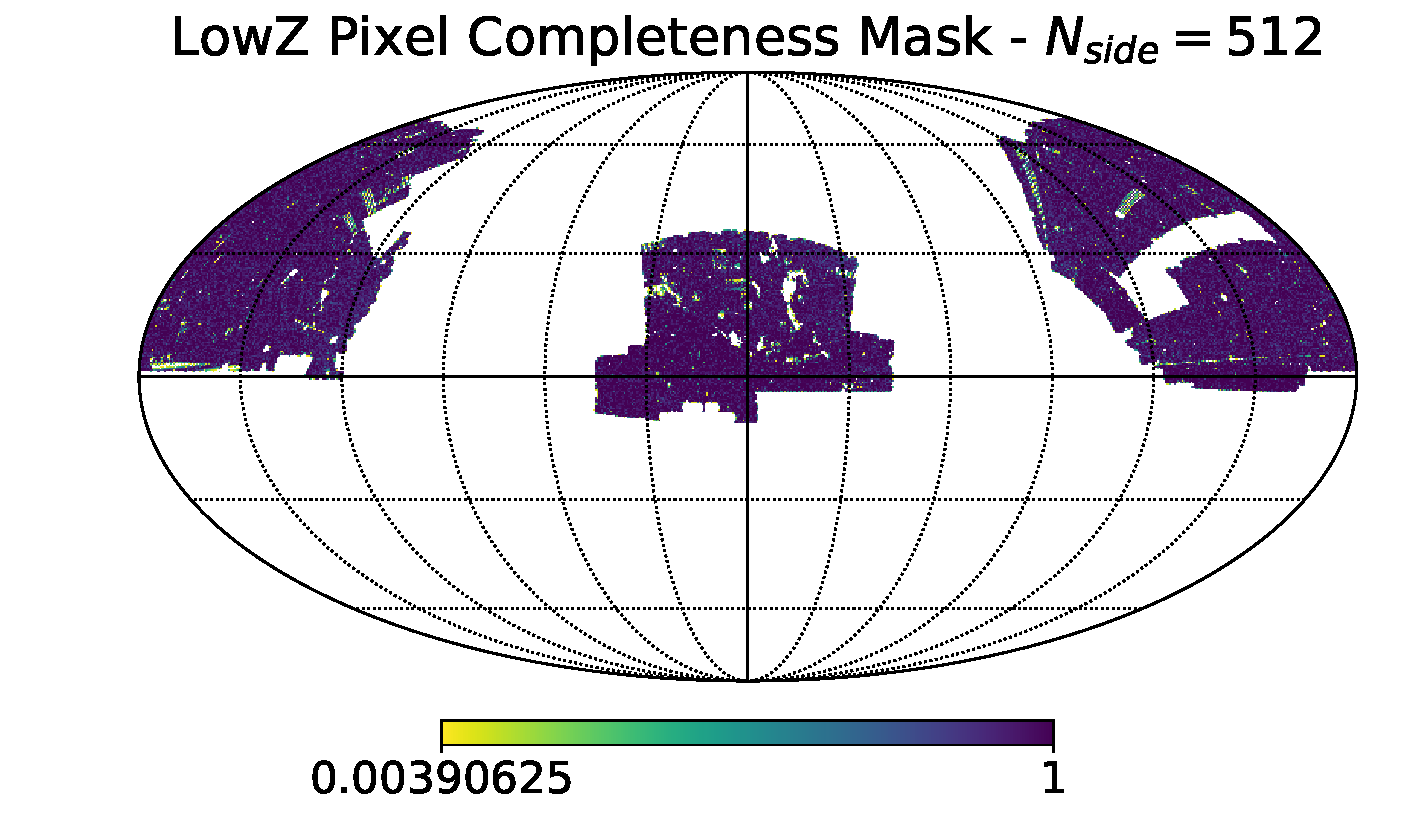
\includegraphics[width=\linewidth]{BOSS-FIGS/LOWZ_Mask}\label{fig:LOWZ_Mask}
\end{subfigure}%
\begin{subfigure}{.5\textwidth}
  \centering
  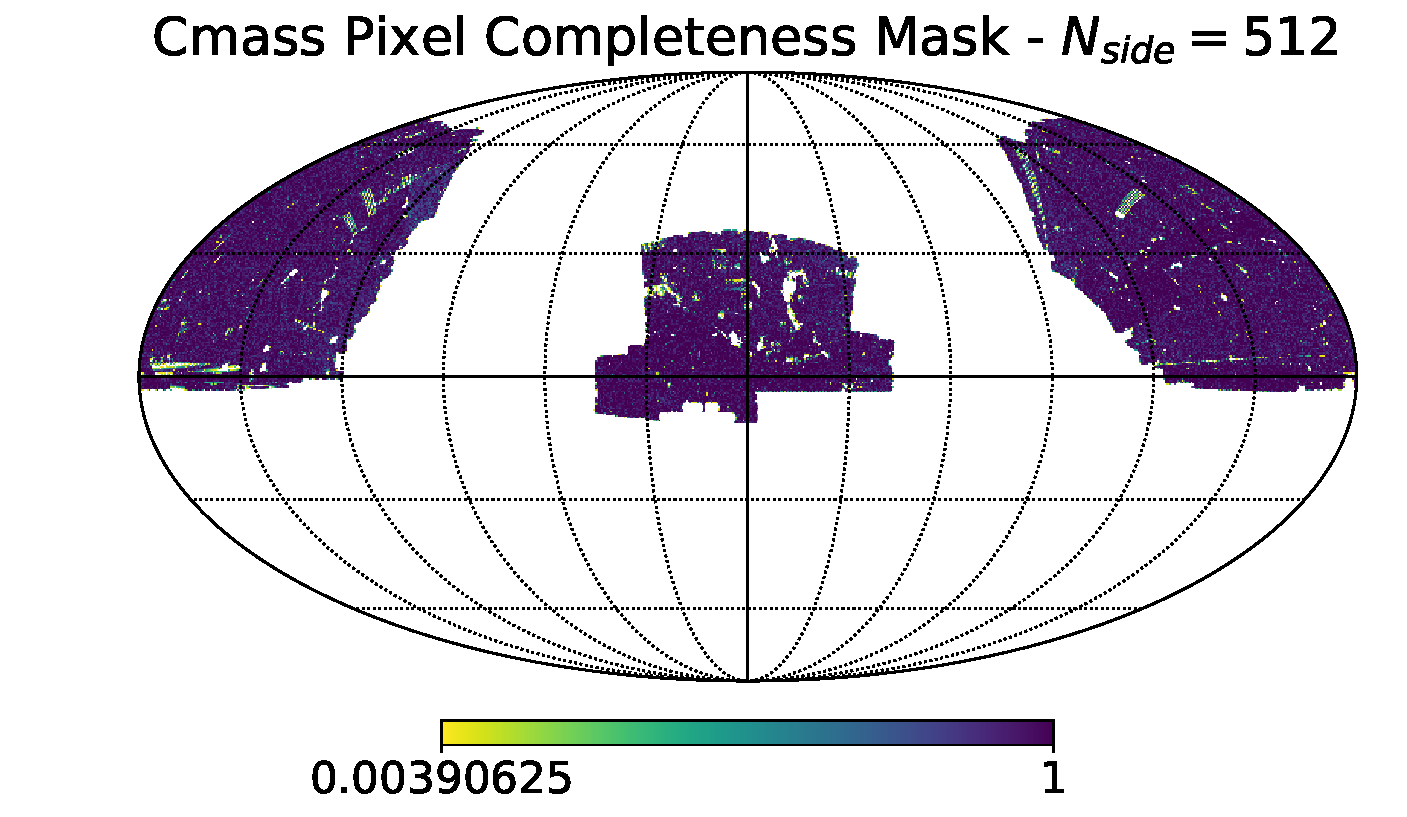
\includegraphics[width=\linewidth]{BOSS-FIGS/CMASS_Mask}\label{fig:CMASS_Mask}
\end{subfigure}
\caption[LOWZ and CMASS angular selection function masks.]{{\small \textit{(left)} LOWZ final pixel completeness angular mask with $N_{side}= 512$. I excluded the LOWZE2 and LOWZE3 regions (the holes in the NGC) due to the non-standard $N(z)$ in these regions (the result of an initially different observing strategy that affected these regions). After performing a pixel completeness cut of $0.8$, the total used area of the mask is around $8529.58\deg^2$ ($f_{sky} = 0.2067$). \textit{(right)}  CMASS final pixel completeness angular mask with $N_{side}=512$. After performing a pixel completeness cut of $0.8$, the total used area of the mask is around $9444.63\deg^2$ ($f_{sky} = 0.2286$). }}
\label{fig:Masks}
\end{figure}

The BOSS collaboration provides\footnote{\url{http://data.sdss3.org/sas/dr12/boss/lss/}} an acceptance mask and several veto masks; these are in \mangle format \citep{2008Mangle}. The acceptance mask is continuous (i.e., takes values between 0 and 1), the value for a given region reflecting the completeness of observations there; in other words, the extent to which spectra were obtained for all targets. The precise value is given by:

% The BOSS collaboration team provides the \mangle \citep{2008Mangle} acceptance and veto masks based on the completeness of each observed tilling, centerpost collisions, collision priority, bright stars, bright objects, seeing cuts, extinction cuts, and other observational factors (for more details, check section 5.1 from \cite{BOSSCatalogue2016}). I downloaded the \texttt{MANGLE} files from the BOSS database \footnote{\textsf{http://data.sdss3.org/sas/dr12/boss/lss/}} and converted the great circle coordinates from the \texttt{MANGLE} polygons to declination and right ascension in order to convert it to a \texttt{HEALPIX} pixelisation scheme using a $N_{side}$ of 8192 ($N_{pix} = 12\times N_{side}^2$). The acceptance mask and the veto masks are then merged at this high resolution \texttt{HEALPIX} scheme, and a hard cut is performed on the completeness of the acceptance mask, $C_{BOSS} > 0.7$, before merging them -- accepted pixels = 1; rejected pixels = 0.
\begin{equation}
C_{BOSS} = \frac{N_{obs}+N_{cp}}{N_{obs}+N_{cp}+N_{\text{missed}}} \ ,
\end{equation}

\noindent where:

\begin{itemize}
\item $N_{obs}$ is the number of spectroscopically observed objects including galaxies, stars, and unclassified objects; 
\item $N_{cp}$ is the number of close-pair objects;
\item $N_{\text{missed}}$ is the number of targeted objects with no spectra.
\end{itemize}

\qquad The veto masks are binary maps (i.e., regions are marked as either good or bad); these maps mask out regions affected by observational factors such as centerpost collisions, collision priorities, bright stars, bright objects, seeing cuts, extinction cuts, and others (see Section 5.1 in \cite{BOSSCatalogue2016}).

\qquad The BOSS acceptance and veto masks are transformed into a high resolution \healpix pixelisation with $N_{side} = 16384$. Using this pixelisation scheme, I combine the BOSS masks to yield a high resolution binary mask. This is done by accepting pixels in which the acceptance mask value $C_{BOSS}$ exceeds 0.7 and which are not marked as bad in any of the veto masks; other pixels are rejected. This choice of completeness cut is based on the BOSS LSS catalogue algorithm from \cite{BOSSCatalogue2016}. This high resolution binary mask is then degraded to a lower resolution ($N_{side} = 512$) continuous mask with values $C_{pix}$ (the \textit{pixel completeness factor}), defined for a given pixel to be the fraction of high resolution sub-pixels that are marked as good in the high resolution binary mask. This is the final mask product and can be seen in figure \ref{fig:Masks} for LOWZ and CMASS. The masks used for the pseudo angular power spectrum estimator (PCL) measurements in Section \ref{Sec:Measurements} contains a hard cut in $C_{pix} \geq 0.8$: values $< 0.8$ are set to 0 and values $\geq 0.8$ are set to 1.

%------------------------------------------------------------------------%
%                        		MAP MAKING
%------------------------------------------------------------------------%
\begin{table}
\centering
\caption[Tomographic redshift bins limits, number of galaxies, and shot-noise levels.]{Details of each redshift tomographic bin containing information on redshift limits, number of objects, and shot-noise value. Note that the shot-noise is calculated after applying the galaxy weights (Section \ref{Sec:GalWeights}, equation \eqref{Eq:Weights}).}
\label{Tb:Shells}
\begin{tabular}{lllcl}
\hline
\hline
Sample Bin & $z_{min}$ & $z_{max}$ & \# of galaxies & Shot-Noise \\ & & & & (gal/strd)$^{-1}$ \\
\hline 
\hline
LOWZ--0  & 0.15      & 0.20      &   43,265   & $6.143 \times 10^{-5} $\\
LOWZ--1  & 0.20      & 0.25      &   51,271   & $5.156 \times 10^{-5} $\\
LOWZ--2  & 0.25      & 0.30      &   59,713   & $4.416 \times 10^{-5} $\\
LOWZ--3  & 0.30      & 0.35      &   85,394   & $3.064 \times 10^{-5} $\\
LOWZ--4  & 0.35      & 0.40      &   83,537   &  $3.136\times 10^{-5} $\\
LOWZ--5  & 0.40      & 0.45      &   57,165   &  $4.605 \times 10^{-5} $\\
CMASS--6 & 0.45      & 0.50      &   177,383  &  $1.577\times 10^{-5} $\\
CMASS--7 & 0.50      & 0.55      &   217,636  &  $1.275\times 10^{-5}$ \\
CMASS--8 & 0.55      & 0.60      &   179,571  &  $1.545\times 10^{-5}$ \\
CMASS--9 & 0.60      & 0.65      &   114,398  &  $2.435 \times 10^{-5}$ \\
CMASS--10 & 0.65      & 0.70      &   57,537   &  $4.850 \times 10^{-5}$ \\
CMASS--11 & 0.70      & 0.75      &   23,631   &  $1.182 \times 10^{-4}$ \\
CMASS--12 & 0.75      & 0.80      &    7,253   &  $3.839 \times 10^{-4}$\\
\hline
\hline
\end{tabular}
\end{table}

\subsubsection{Healpix overdensity maps:}\label{Sec:Maps}
%From the galaxy catalogues, the final data products to be used in the analysis are galaxy overdensity \texttt{HEALPIX} maps. In order to produce them, first I properly bin both data catalogues into redshift tomographic bins of $\Delta z = 0.05$. This results in 6 tomographic bins for LOWZ, from $z \geq 0.15$ to $z=0.45$; and 7 tomographic bins for CMASS, from $z \geq 0.45$ to $z = 0.80$. Details about each redshift bin can be found in table \ref{Tb:Shells}. Next, using \texttt{HEALPIX}'s \texttt{ANG2PIX} function, I create a \textit{weighted number counts} map which contains the number of objects in each \texttt{HEALPIX} pixel, $n_p$, weighted by the \textit{total galaxy weight} given by equation \eqref{Eq:Weights}. To create the final galaxy overdensity maps, I need to up-weight the $n^g_p$ maps according to the pixel completeness from the masks, $C_{pix}$ -- a second and different up-weighting than the one presented in Section \ref{Sec:GalWeights}. Here, objects in pixels with $C_{pix} <  0.8$ are now considered outside the footprint, \textit{i. e.} the pixel value is set to zero. Thus, the expression for the overdensity maps is:
 From the galaxy catalogues, I generate the final data products to be used in the analysis: the galaxy overdensity \healpix maps. First, I bin both data catalogues into tomographic redshift bins of $\Delta z = 0.05$. This gives six tomographic bins for LOWZ ($0.15 \leq z < 0.45$) and seven for CMASS ($0.45 \leq z < 0.80$). Details about each redshift bin can be found in table \ref{Tb:Shells}. According to \cite{Asorey2012}, $\Delta z = 0.05$ is the thickest possible redshift bin size a spectroscopic redshift survey with $z < 1$ can have in order to keep sufficient radial information without suppressing the radial BAO information due to averaging originating from mode projection. Smaller bin sizes could improve the quality of radial information; however, the trade-off between bin size and shot-noise per bin for the case considered in this chapter is such that the shot-noise would then be too high for the considered scales. The use of the cross-power spectra between adjacent bins allows for RSD information to be properly probed as explained in Section \ref{Sec:RSD}.

\qquad Next, I create a \textit{weighted number counts} map which contains the number of objects in each \healpix pixel, $n_p$, weighted by the \textit{total galaxy weight} ($w_{tot}$) given by Equation \eqref{Eq:Weights}. To create the final galaxy overdensity maps, I up-weight the maps by the inverse of the pixel completeness factor from the masks, $C_{pix}$. Here, objects in pixels with $C_{pix} <  0.8$ are now considered outside the footprint, i.e. the pixel value is set to zero. Thus, the expression for the overdensity maps is:

\begin{equation}
\delta_{z,p}^g = 
\begin{cases}
\left(\frac{1}{C_{pix,p}}\frac{n^g_{z,p}}{\bar{n}_z}\right) - 1 & \text{, if } C_{pix,p} > 0.8 \\
0 & \text{, otherwise}
\end{cases}
\label{Eq:OverDMaps}
\end{equation}
where $\bar{n}_z$ is the mean number of weighted galaxies per observed pixel, in each redshift tomographic bin. Note that the weight I am referring here are the one mentioned in Equation \ref{Eq:Weights}, the $\bar{n}_z$ is not weighted by the pixel completeness weight.  After these procedures are applied to all 13 redshift tomographic bins, the data products are ready for the power spectra of these maps to be measured using the Pseudo-$C_{\ell}$ estimator described on the next sections.

%------------------------------------------------------------------------%
%                      EESTIMATORS AND MEASUREMENTS
%------------------------------------------------------------------------%
\section{Angular Power Spectra Estimators and Measurements}\label{Sec:Measurements}
The first proposed method for estimating the angular power spectrum $C_{\ell}$  \citep{Peebles1973} consists of projecting the density field onto the celestial sphere, decomposing this projected field into spherical harmonics, and then analysing statistically the coefficients of this decomposition. I refer here to this method of estimating the power spectrum as a \textit{pseudo power spectrum estimator} (PCL). This is a widely used tool for both galaxy clustering and CMB analysis and explored in several different approaches in the literature (see before-mentioned works).

\subsection{Pseudo-$C_{\ell}$ Estimator}\label{Ref:PCL}

Here, I describe the PCL estimator, following recent approaches as presented in e.g. \cite{ScharfLahav1992}, \cite{FisherLahav1994}, \cite{Wright1994}, \cite{2001Huterer}, \cite{PolSpice2001}, \cite{BlakeFerreira2004}, \cite{Blake2007}, \cite{Thomas2010Neutr}, \cite{Thomas2011b}, \cite{Thomas2011}, and \cite{Ho2012}. The aim is to measure the angular power spectrum of the galaxy overdensity field, $\delta^g$. 

\qquad Let $\bar{\rho}^g$ be the average of $\rho^g$ over the sky and define the galaxy overdensity field to be  

\EQ{}{
\delta^g = \frac{\rho^g - \bar\rho^g }{\bar\rho^g } = \frac{\rho^g }{\bar\rho^g} -1,}

\noindent This field may be represented using spherical harmonic expansion:

\EQ{}{
\delta^g(\theta, \phi) = \sum_{\ell=0}^{\ell_{max}} \sum_{m=-\ell}^{\ell} d_{\ell m} Y_{\ell m}(\theta, \phi),}

\noindent where the spherical harmonic coefficients $d_{\ell m}$ are defined by

\EQ{}{
d_{\ell m} = \int \delta^g(\theta,\phi) Y_{\ell m}^*(\theta,\phi) d\Omega.}

\noindent Here and in what follows, a coordinate system is fixed, $(\theta, \phi)$, for the celestial sphere; the spherical harmonic functions are defined with respect to this coordinate system. The estimator of the angular power spectrum of the data is then

\EQ{}{
\hat{D}_{\ell} = \frac{1}{2\ell +1} \sum_{m = -\ell}^{\ell} d_{\ell m}^{} d_{\ell m}^{\ast}.}

\noindent The averaging over $m$ is motivated by the assumed isotropy of the probability distribution governing the location of galaxies.

\qquad To handle the partial-sky case, let $\Omega_{tot}$ be the survey region and define

\EQ{Jlm}{
J_{\ell m} = \int_{\Omega_{tot}} \left|Y_{\ell m} \right|^2d\Omega \ .}

\noindent This is a normalization factor due to the average of modes in the partial sky coverage; note that $J_{\ell m}=1$ for a full-sky survey. There will also be a term correcting for bias introduced by the partial sky measurement. However this term is proportional to the average field value; in the case considered this average vanishes, so the bias correction need not be made. See Appendix \ref{Apx:PCL} for details. 

\qquad One can repeat this analysis for galaxy density fields $\rho^{g, i}$ and $\rho^{g, j}$ defined in tomographic bins $i$ and $j$. Combining the partial sky effect and tomographic binning results in an estimator $\hat{D}_{\ell}^{i j}$ for the cross- $(i \neq j)$ or auto- $(i = j)$ power spectrum of the data

\EQ{D_hat}{
\hat{D}_{\ell}^{i j} = \frac{1}{2\ell +1} \sum_{m = -\ell}^{\ell}D^{ij}_{\ell m}}

\noindent where

\EQ{D_lm_ij} {
D^{ij}_{\ell m} = \frac{\Re(d_{\ell m}^i d_{\ell m}^{j \ast})}{J_{\ell m}}.
}

\noindent Here, I take the real part $\Re()$ of a quantity whose expectation value will have no imaginary part. 

\qquad In reality one works with a pixelised celestial sphere and measure not $\rho^g$ but rather a galaxy count $n^g_p$ per pixel $p$. From this one can derive the per-pixel galaxy overdensity

\EQ{define_delta_p}{
\delta^g_p = \frac{n^g_p}{\Delta \Omega_p} \frac{\Delta \Omega_{tot}}{n^g_{tot}} - 1,}

\noindent where $n^g_{tot}$ is the total galaxy count, $\Delta \Omega_p$ the solid angle subtended by pixel $p$, and $\Delta \Omega_{tot}$ the total solid angle of the survey region $\Omega_{tot}$.

\qquad On the pixelated sphere, the spherical harmonic coefficients are estimated by

\EQ{AlmPix}{
d_{\ell m} = \sum_p \delta^g_p Y_{\ell m}^{\ast}(\theta_p,\phi_p) \Delta\Omega_p ,}

\noindent where $(\theta_p,\phi_p)$ are the coordinates at the centre of pixel $p$, $\Delta\Omega_p$ is the area of $p$, and the sum is over all pixels in the survey region.

\qquad Pixelisation is a smoothing operator, and hence suppresses power at small scales. I now summarise here the standard treatment of this effect; see \cite{Healpix,Boris2013} and the \healpix documentation for details\footnote{For details on the pixel window function: \url{https://healpix.jpl.nasa.gov/html/intronode14.htm}}. Consider the contribution of a given pixel $p$ to $d_{\ell m}$ both for the (measured) pixelised field and for the (desired) ideal continuous field; the ratio of these quantities is 

\EQ{}{
w_{\ell m}^p = \frac{\int_p Y_{\ell m}(\theta,\phi) d\Omega}{Y_{\ell m}(\theta_p,\phi_p) \Delta \Omega_p}.}

\noindent This quantity depends sensitively on $\ell$: for small $\ell$, $Y_{\ell m}$ is slowly varying and hence $w_{\ell m}^p$ will be close to unity while for large $\ell$ the rapidly varying $Y_{\ell m}$ will have vanishing integral over $p$. However the dependence on $m$ and $p$ will be small and can be averaged out (in quadrature), yielding:

\EQ{}{
w_{\ell}^2 = \frac{1}{N_{pix}(2\ell+1)} \sum_{p,m} \left| w_{\ell m}^p \right|^2.}

\noindent The ratio of the power spectra of the (measured) pixelised overdensity field to that of the (desired) continuous field will then be $w_{\ell}^2$. This study uses a \healpix resolution of $N_{side} = 512$; which means that at $\ell_{max} = 510$ this ratio of powers ($C_{\ell}^{pix}/C_{\ell}^{unpix}$) is then $0.911$ due to the pixel window function.

\qquad Galaxy clustering observations contain both signal and (Poisson) noise; spatial variations in the latter contribute to the measured auto power spectrum and this effect must be removed when estimating the power spectrum of the underlying signal. 

\qquad As the signal and noise are uncorrelated, the angular power spectra of the signal ($S_{\ell}$), data ($D_{\ell}$) and noise ($N_{\ell}$) are related by:

\EQ{SignalNoise}{
S_{\ell} = D_{\ell} - N_{\ell}.}

\qquad For most tomographic bins one can approximate the angular power spectrum of the noise as the variance of a Poisson distribution:

\EQ{NoiseNl}{
N_{\ell} \approx \frac{\Delta\Omega_{tot}}{n^g_{tot}} = \frac{1}{\bar{n}},}

\noindent where $\bar{n}$ is the mean number of galaxies per steradian.

\qquad Amending \eqref{Eq:D_hat} to account for pixelisation and shot-noise yields an estimator $\hat{S}^{ij}_{\ell}$ for the partial sky signal power spectrum between two redshift bins \textit{i} and \textit{j}:

\EQ{Sl_wl}{
\hat{S}^{ij}_{\ell} = \frac{1}{w_{\ell}^2} \left[ \left(\frac{1}{(2\ell+1)}\sum_{m=-\ell}^{\ell} D^{ij}_{\ell m}\right) - N_{\ell}\delta_{ij}\right].}


\noindent The estimator is symmetric in $i$ and $j$. Note also that there is no shot-noise contribution for the cross-power spectra ($i \neq j$). The PCL estimator described here uses galaxy overdensity maps instead of the galaxy counts maps used in \cite{Blake2007,Thomas2011} and others; Appendix \ref{Apx:PCL} describes the correspondence between the two approaches. This estimator is unbiased \citep{Peebles1973} but does not have minimum variance: maximum likelihood estimators such as QML \citep[e.g.][]{Efstat2004} have smaller variance. However, these maximum likelihood estimators are computationally expensive to use; this is why this work uses PCL. %The same is valid for the Bayesian estimator considered in chapter \ref{chap:BPL} and some extra complications related to extracting cosmological information from its full posterior are also discussed in the relevant chapter.

\begin{figure*}
\begin{center}
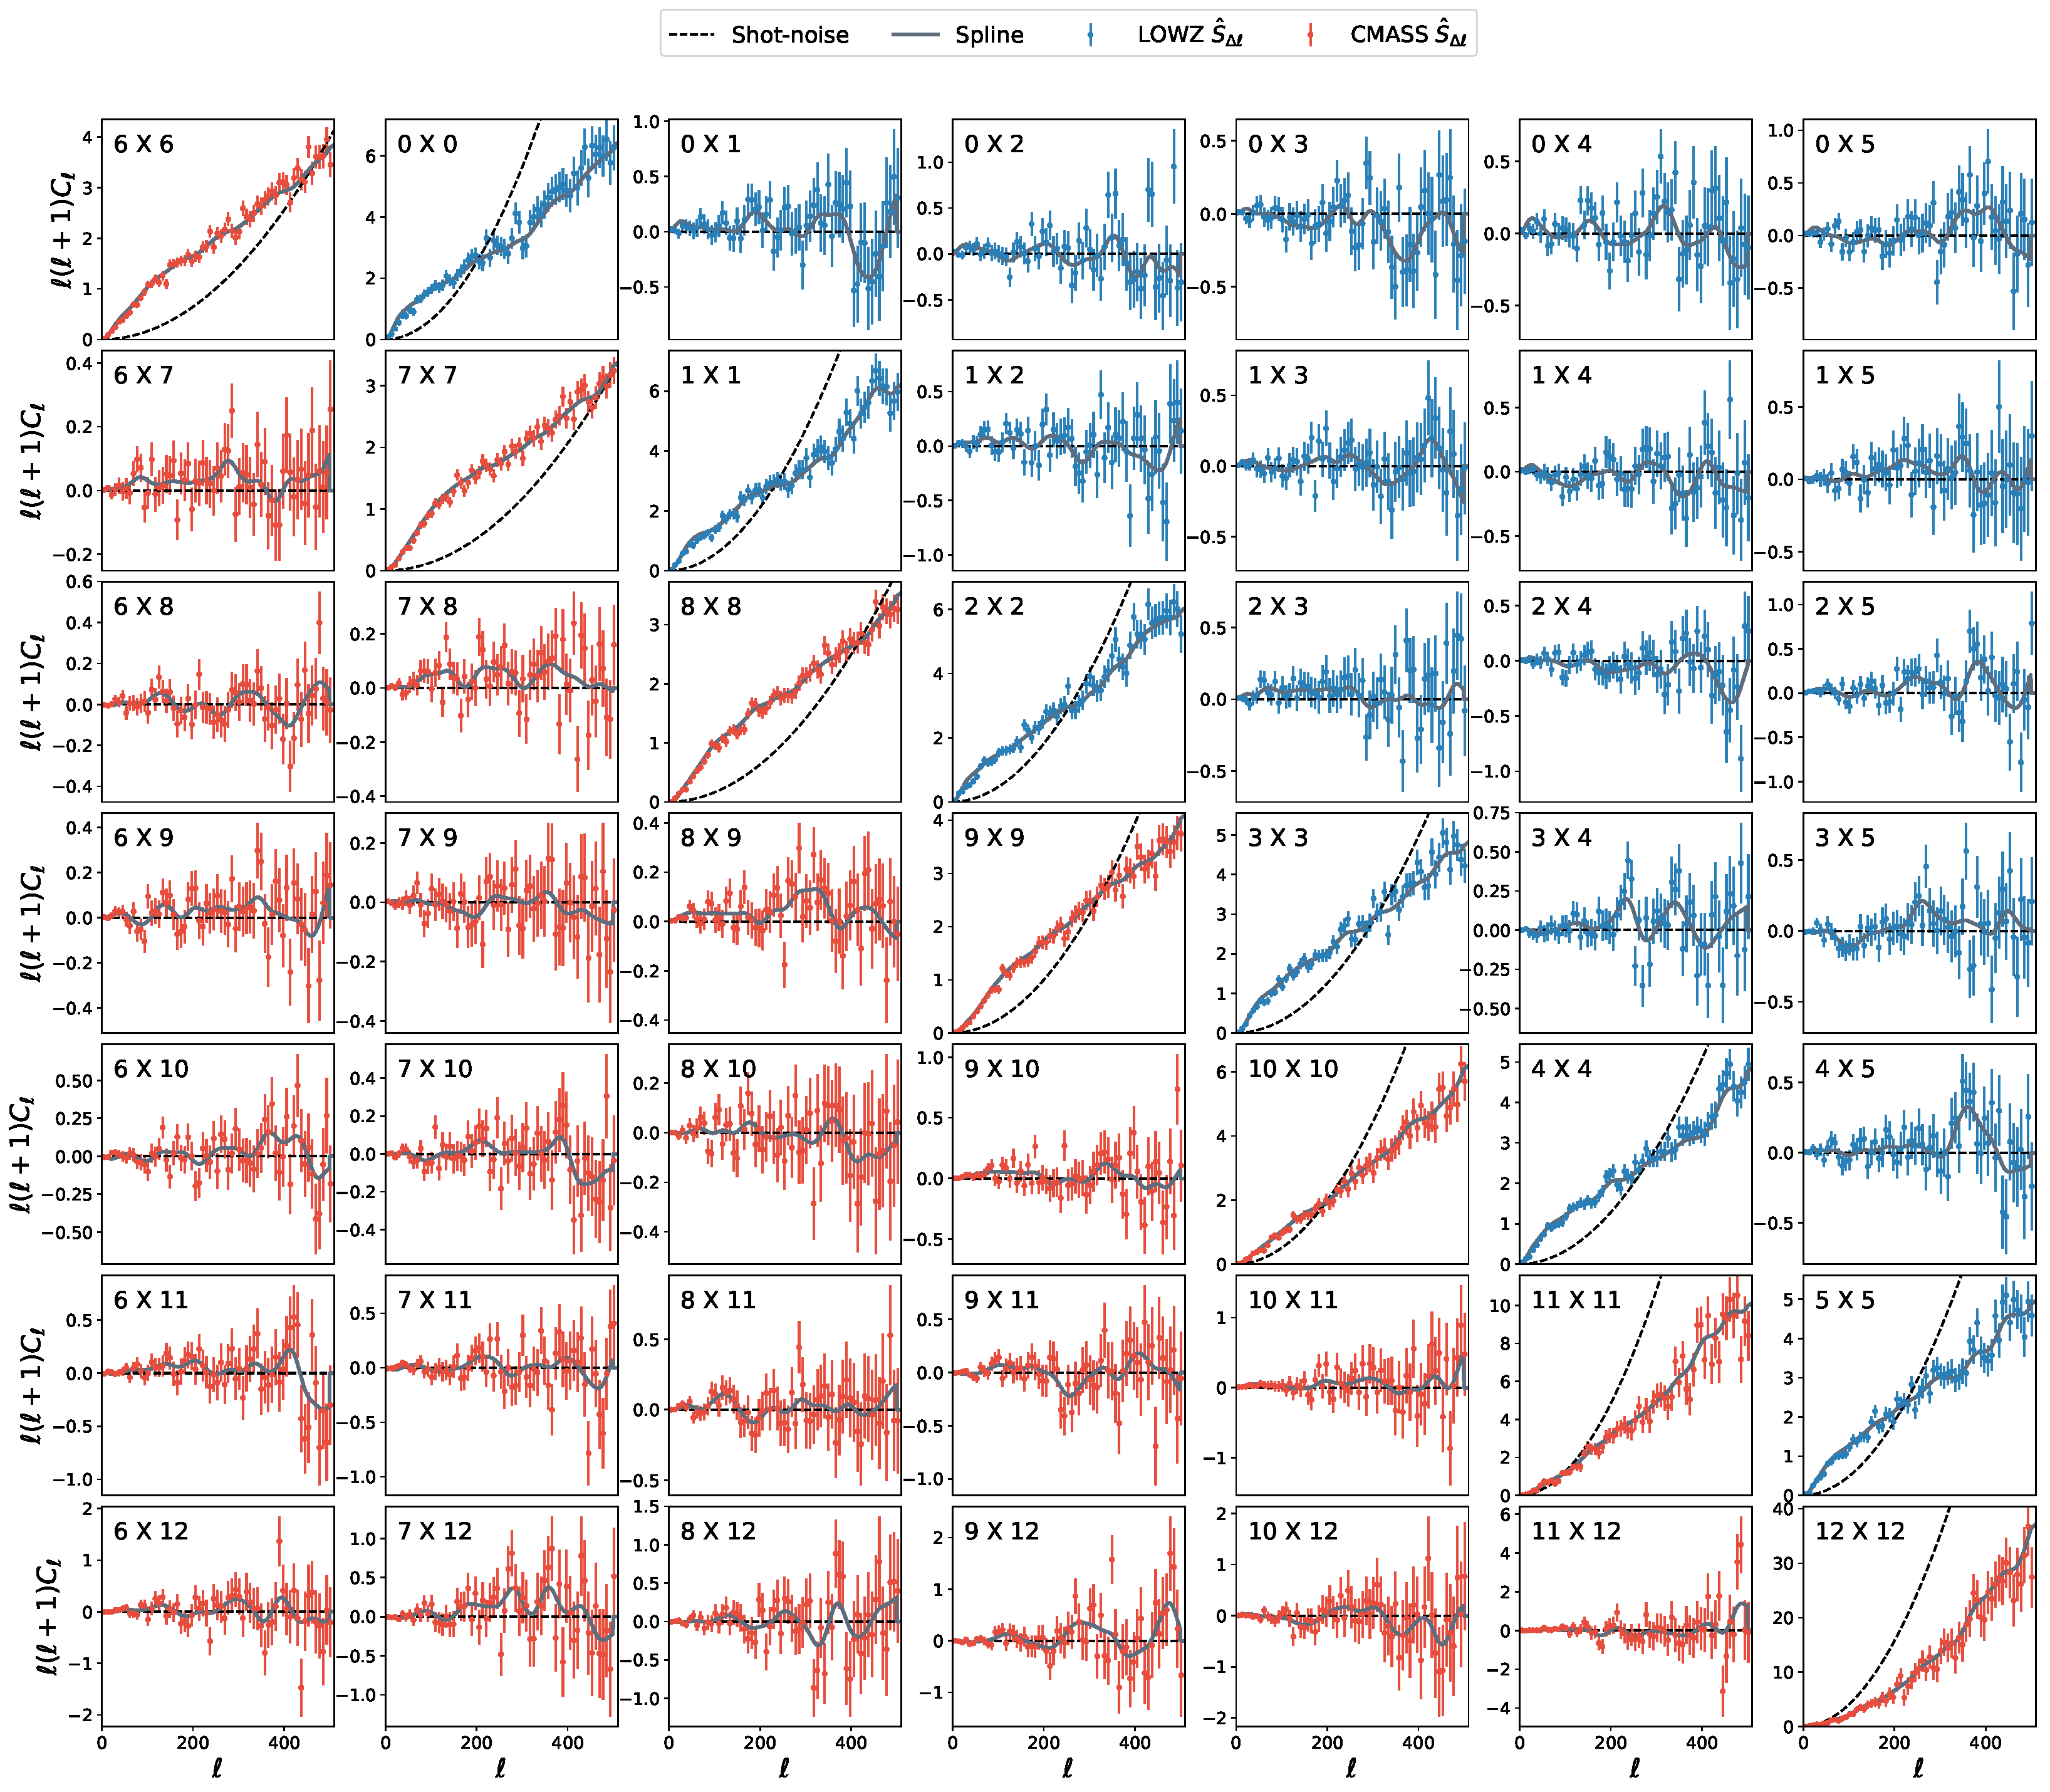
\includegraphics[width=1.0\textwidth]{BOSS-FIGS/PCL-data_red3.pdf}
\caption[Measured angular power spectra from the BOSS samples.]{Measured signal auto- and cross-power spectra for the LOWZ (blue) and CMASS (red) samples (Equation \ref{Eq:S_delta_ell}). The black dashed lines show the estimated Poissonian shot-noise (Equation \ref{Eq:NoiseNl}). The solid grey line shows the deconvolved spline used in Section \ref{Sec:Cov} to generate the log-normal mocks for covariance matrix estimation from which the error bars in this figure were estimated. Even though the measured $\hat{S}_{\Delta\ell}$ had the shot-noise removed, note that the last two CMASS bins have a significant part of their signals below the level of Poissonian shot-noise.}
\label{fig:PCLs}
\end{center}
\end{figure*}

\subsection{Bandwidth Binning and Measurements}

The measurements are binned in $\ell$ using bins of width $\Delta\ell = 8$ (so e.g. the first bin is $2 \leq \ell \leq 9$). For each bin, I calculate a weighted average of the $\hat{S}_{\ell}^{ij}$ (weighted by the number of spherical harmonic coefficients):

\EQ{S_delta_ell}{
\hat{S}_{\Delta\ell}^{ij} = \frac{\sum_{\ell \in \Delta\ell}(2\ell+1)\hat{S}_{\ell}^{ij}}{\sum_{\ell \in \Delta\ell}(2\ell+1)} \ .}

\noindent This binning acts on the measurement in a way that decorrelates mixed modes (that arise from the convolution of the true measurement and the survey's angular window function). 

\qquad Finally, I measure the PCL estimator up to $\ell_{max} = 510$; Figure \ref{fig:PCLs} shows the results for the auto- and cross-power spectra for LOWZ and CMASS. Note that I do not consider in this work any cross-correlations between the two samples; therefore, each sample is treated individually. The figure also shows error bars given by the diagonal of the covariance (estimated in Section \ref{Sec:Cov}), as well as the splines used to generate the log-normal mocks (Section \ref{Sec:Cov}). The figure shows that the last two CMASS bins are dominated by shot-noise (due to their small density of galaxies). Uncertainty in the characterisation of this noise will be included into the theoretical forward modelling presented in Section \ref{Sec:Theory} and marginalised over during the cosmological parameter estimation (Section \ref{Sec:CosmoBananas}).



%------------------------------------------------------------------------%
%                      THEORY CLS AND COVARIANCE MATRIX
%------------------------------------------------------------------------%
\section{Theory Modelling and Covariance Matrix Estimation}\label{Sec:Theory}
This work's goal is to use observations to constrain cosmological parameters; as part of this, I describe the theory that connects the statistics of the underlying matter field with the measured angular power spectra. My approach is similar to that found in the literature \citep{ScharfLahav1992,2001Huterer,Padm2007,Thomas2011,Asorey2012}.

\qquad In this section, I outline the framework necessary to obtain the desired cosmological parameter's constraints from the measured angular power spectra.  I detail here the theoretical framework used to estimate the theory vector, the procedure used to build covariance matrices from log-normal mocks, and the theoretical expression for the covariance of the PCL estimator.

\subsection{Theoretical Angular Power Spectra}
Let $\delta_{g}(\textbf{x},z)$ denote the galaxy density function. Let $\delta_{g}(\textbf{k},z)$ be its Fourier transform; one can write this in terms of the growth function $D(z)$, the bias $b(z)$ (assumed here to be scale-independent), and the Fourier components $\delta(\textbf{k},0)$ of the underlying matter distribution at the current time:

\begin{equation}
\delta_g(\textbf{k},z) = D(z)\delta_g(\textbf{k}) = D(z)b(z)\delta(\textbf{k},0).
\end{equation}

%\noindent The correlation structure of the Fourier transform is
\noindent The correlation structure of the Fourier transform is

\begin{equation}
\langle \delta_{g}(\textbf{k},z) \delta_{g}^*(\textbf{k}',z) \rangle = (2\pi)^3\delta^{(D)}(\textbf{k}-\textbf{k}')P_g(k,z) \
\end{equation}

\noindent where $P_g(k,z) = b(z)^2P(k,z)$ is the power spectrum of the galaxy density field and $P(k,z)$ is the power spectrum of the underlying matter density field. 

\qquad Integrating the galaxy density along the line of sight, $\hat{\textbf{n}}$, yields:

\begin{equation}
\delta_g(\hat{\textbf{n}}) = \int_0^\infty \delta_g(\chi(z)\hat{\textbf{n}}, z) n(z) dz
\end{equation}
%\begin{ceqn}\begin{equation}
%\delta_g^{2D}(\ell) = i^l\int \frac{d^3k}{(2\pi)^3}\delta(z,\textbf{k})W_{g,\ell}(k).
%\label{Eq:Delta2D}
%\end{equation}\end{ceqn}
where $n(z)$ is the normalised redshift-dependent selection function and $\chi(z)$ is the comoving distance. The spherical harmonic components $a_{\ell m}$ of this projected galaxy distribution are:

\begin{align}
a_{\ell m} &= \int Y_{\ell m}(\hat{\textbf{n}}) \delta_g(\hat{\textbf{n}}) d\Omega \\
		&= \int Y_{\ell m}(\hat{\textbf{n}}) \int \delta_g(\chi(z)\hat{\textbf{n}},z) n(z) dz d\Omega \\
        &= \frac{4\pi}{(2\pi)^3} \int b(z)n(z)D(z) \int \delta(\textbf{k},0) i^{\ell} j_{\ell}(k\chi(z)) Y_{{\ell},m}(\hat{\textbf{k}}) d^3k dz.\label{Eq:ThisOne}
\end{align}
where $j_{\ell}(k\chi(z))$ are the Spherical Bessel functions \citep{Thomas2010Neutr, Thomas2011}.

\begin{figure}
\begin{center}
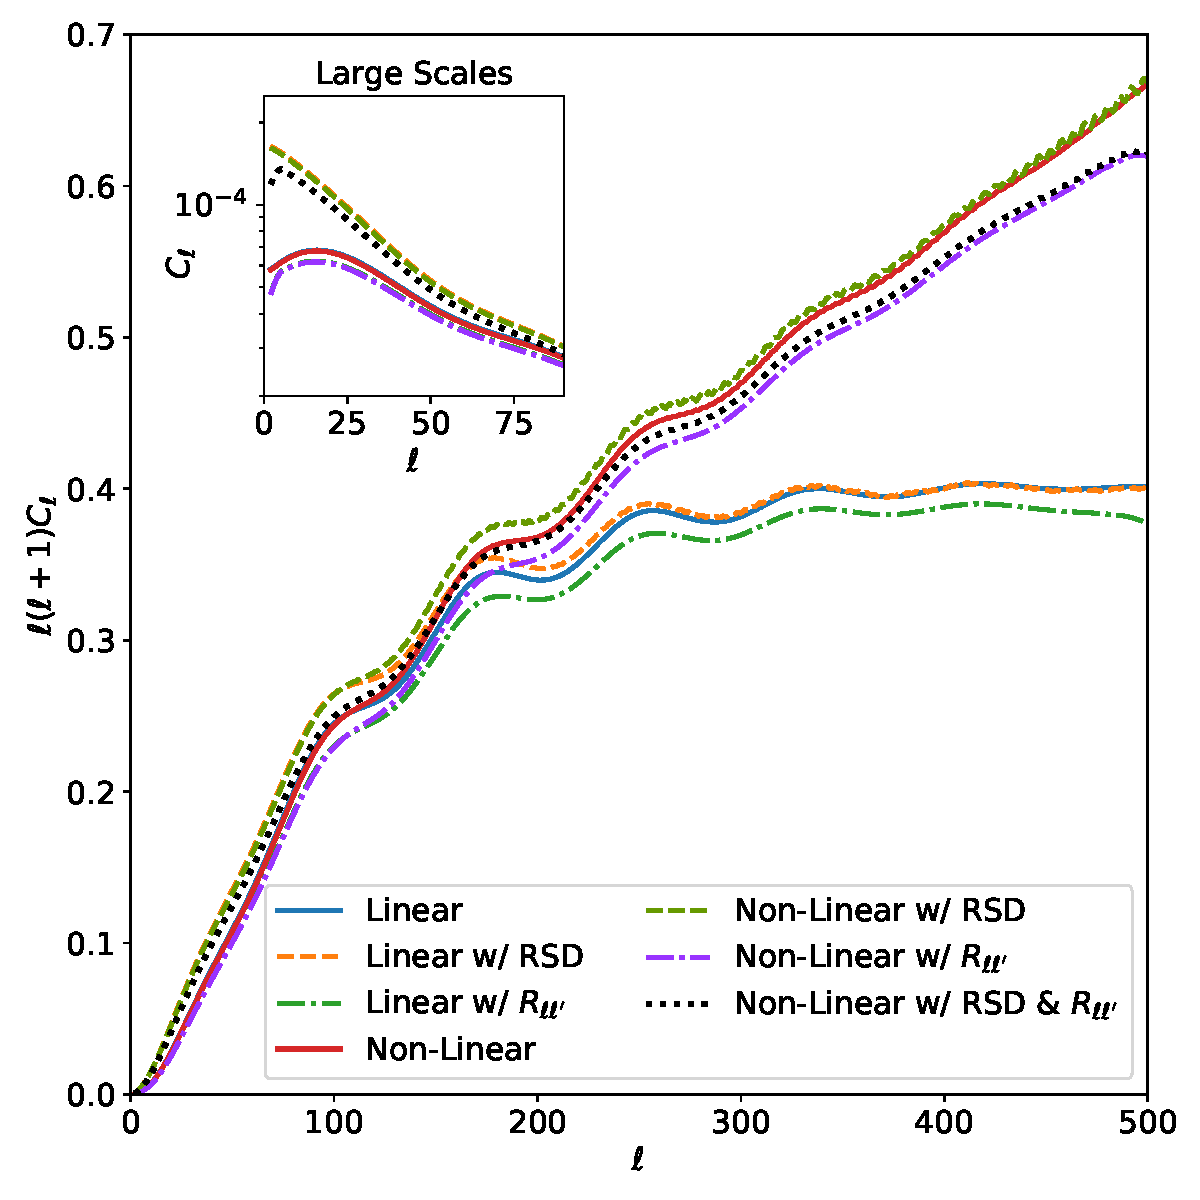
\includegraphics[width=\textwidth]{BOSS-FIGS/Cls-Comparison.pdf}
\caption[Different effects which affect the angular power spectrum modelled into \texttt{UCLCL}.]{A series of different effects which affect the angular power spectrum ($0.45 < z \leq 0.50$) in a variety of ways. The two \textit{solid lines} show the linear and non-linear $C_{\ell}$'s (Section \ref{Sec:NonLin}) which diverge as a function of scale, $\ell$. \textit{Dashed lines} include the Redshift space distortions effect (Section \ref{Sec:RSD}) which increases the power for larger scales (see sub-panel). \textit{Dot-dashed lines} show the effect of the mixing matrix convolution (Section \ref{Sec:MixingMat}) which tends to suppress power in all scales. Finally, the black dotted line is a combination of all such effects: RSDs, non-linearities, and mixing matrix convolution. The input parameters for these calculations were done using a flat cosmology: $b=1$, $h = 0.6725$, $\Omega_b = 0.0492$, $\Omega_{cdm} = 0.265$, $w_0=-1.0$, $\tau_r = 0.079$, $\log A_s = 3.093 \times 10^{-10}$, $n_s = 0.965$. These theory lines were all generated using the \uclcl code.}
\label{fig:Cl_Theory}
\end{center}
\end{figure}

\noindent The final step uses the plane wave expansion and the spherical harmonic addition theorem. One may collect the $z$ dependencies from Equation \eqref{Eq:ThisOne} into a window function:

\begin{equation}
W_{g,\ell}(k) = \int b(z) n(z)D(z)j_{\ell}(k\chi(z)) dz.\
\end{equation}

\qquad Using the window function in Equation \eqref{Eq:ThisOne} yields a simple expression for the angular power spectrum:

\begin{align}
C_{\ell}^{ij} & \equiv \left\langle a_{\ell m}^i a_{\ell m}^{j*} \right\rangle \\
& = \frac{2}{\pi} \int W^i_{g,\ell}(k)W^j_{g,\ell}(k)k^2 P(k,0) dk.
\label{Eq:ClTheoretical}
\end{align}

\noindent Here I have introduced superscripts $i$ and $j$ to denote different redshift shells and the equation above, therefore, defines both auto-$C_{\ell}$ (for $i = j$) and cross-$C_{\ell}$ (for $i \neq j$). The same formalism can be used to obtain the $C_{\ell}$ between two different tracers, between photometric and spectroscopic redshift shells, etc.

\qquad In this work, I used the Unified Cosmological Library for $C_{\ell}$s, or \uclcl code (Cuceu et al, in prep). This code obtains the primordial power spectra and transfer functions from the \class Boltzmann code \citep{Class}, and then applies Equation \eqref{Eq:ClTheoretical} to obtain the angular power spectrum. \uclcl deals with the redshift distribution in more flexible ways than does \class and \camb \citep{CAMB}: it allows for the input $n(z)$ distribution to be a spline and also allows it to be convolved with a Gaussian error function to take into account redshift systematic effects (Equation \ref{Eq:GaussianErrNz} in Section \ref{Sec:SpecNz}). {A comparison between these codes is presented in Appendix \ref{Apx:Code_Comparison}.} %which uses the \texttt{CLASS} Boltzmann code \citep{Class} to obtain the primordial power spectra and transfer functions, and project it to obtain a angular power spectrum as in equation \eqref{Eq:ClTheoretical}. Differently from \class and \camb, \uclcl deals with the redshift distribution in more flexible ways. Among which, \uclcl allows for the input $n(z)$ distribution to be a spline and also to convolve it with a gaussian error function to take into account redshift systematic effects (Equation \ref{Eq:GaussianErrNz} in section \label{Sec:SpecNz}).

%------------------------------------------------------------------------%
%                        RSD AND WINDOW FUNCTION
%------------------------------------------------------------------------%
\subsubsection{Spectroscopic Redshift Distribution and shot-noise modelling:}\label{Sec:SpecNz}
The spectroscopic selection provides a full (un-normalised) $n(z)$ function for both LOWZ and CMASS samples (see Fig. \ref{fig:NZ_BOSS}). Binning is achieved by hard cuts on each of these samples in intervals of $\Delta z = 0.05$ (Section \ref{Sec:Maps}), with no overlap or gaps between bins. Despite the impressive precision of spectroscopy, to suggest that these bins have no overlap (i.e. there is no error in the spectroscopic measurement) is unrealistic, and has a significant impact on the cross correlations between bins. Spectroscopic errors are modelled within the distribution functions by a convolution with a narrow Gaussian function representing the uncertainty on a given measurement. Such a convolution is given by
\begin{equation}
n^i(z) = \int n_*^i(z-z^\prime) e^{-\frac{z^{\prime 2}}{2\sigma_s^2}} \mathop{dz^\prime},
\label{Eq:GaussianErrNz}
\end{equation}
where $n_*^i(z)$ is the raw redshift distribution, $\sigma_s$ (the variance of the Gaussian) is a proxy for the spectroscopic measurement error, and $n^i(z)$ is the final redshift distribution to be used in calculations. In practice, the convolution is achieved by means of a fast Fourier transform (FFT) algorithm, multiplication of the functions, and reverse transform in the \uclcl pipeline.

\qquad This convolution can also be used to approximate a separate effect and more dominant effect, the so called Fingers-of-God (FoG) effect \citep{Percival-FoG2011}; which will actually dominate the measurements on $\sigma_s(z)$ in Equation \eqref{Eq:GaussianErrNz}. This is a form of redshift-space distortion (RSD) which arises as a result of random motions of galaxies within virialised structures, which elongates the appearance of structure in redshift space, i.e., it smears out the redshift distribution by the addition of Doppler shift to cosmological redshift. The convolution width $\sigma_s$ models the combined impact of spectroscopic redshift errors and of the FoG effect; $\sigma_s$ is then varied and marginalised over during the cosmological analysis. Due to the sensitivity of the cross-angular power spectra to these effects, a separate $\sigma_s$ is used for each redshift bin (for more details see Section \ref{Sec:LikelihoodsPriors}).

\subsubsection{Redshift Space Distortions:}\label{Sec:RSD}
The full large scale structure window function needs to take into account Redshift Space Distortions (RSD) \citep{Blake2007,Padm2007,Thomas2011}. This effect tends to increase the power for large scales, $\Delta \ell < 60$, due to the mix of redshift and peculiar velocities of galaxies. This local peculiar motion of galaxies creates the illusion that the ones moving towards us appear closer (i. e., they appear to be at lower redshifts); while galaxies with peculiar motion moving away from us, appear to be ever further away (i. e., they appear to be at lower at higher redshifts). This effect can be easily taken into account by adding the RSD window function  \citep{ScharfLahav1992, FisherLahav1994, Kirk2015, 2016McLeod} to equation \eqref{Eq:ClTheoretical}:

\begin{equation}\label{Eq:Window_counts}
W^{Tot,i}_{\ell}(k) = W^i_{g, \ell}(k) + W^i_{RSD,\ell}(k) \ , 
\end{equation}

where the RSD window function is given by \citep{ScharfLahav1992, Padm2007,Ho2012,Kirk2015}:

\begin{equation}
\begin{split}
%W^i_{RSD,\ell}(k) = & \beta^i \int n^i(z)D(z)\left( \frac{d\chi(z)}{dz} \right)^{-1} \times \\ & \left[ \frac{(2\ell^2 + 2\ell -1)}{(2\ell + 3)(2\ell -1)}j_{\ell}(kz) \right. \\
W^i_{RSD,\ell}(k)  = & \frac{\beta^i}{k} \int d\chi \frac{dn^i}{d\chi} j'_{\ell}(k\chi (x)) \\
 = & \beta^i \int \, n^i(\chi(z))\left[ \frac{(2\ell^2 + 2\ell -1)}{(2\ell + 3)(2\ell -1)}j_{\ell}(k\chi(z)) \right. \\
& \left. + \frac{\ell(\ell-1)}{(2\ell-1)(2\ell+1)}j_{\ell-2}(k\chi(z)) -  \dfrac{(\ell+1)(\ell+2)}{(2\ell+1)(2\ell+3)}j_{\ell+2}(k\chi(z)) \right] d\chi \ ,
\end{split}
\end{equation}

where the redshift distortion parameter, $\beta^i = (d \ln D(z)/d\ln a)/b^{i}(z) \approx \Omega_m^{\gamma}/b^i(z)$, is defined to be dependent on the bias of the given redshift shell or tracer. The RSD window function does not account for the FoG effect, which affects small scales due to the virial motion of galaxies inside clusters \citep{Kang2002}; instead, as discussed in \ref{Sec:SpecNz}, the FoG effect is subsumed into the spread of the spectroscopic redshift distribution.  

\qquad Figure \ref{fig:Cl_Theory} shows the impact on the angular power spectrum of different effects considered in this section: redshift space distortions, non-linearities, and partial sky convolution with the mixing matrix. Some of these effects affect the angular power spectrum from different scales in different redshift ranges consider in this work.

%------------------------------------------------------------------------%
%                        	NON-LINEAR C(L)
%------------------------------------------------------------------------%
\subsubsection{Non-Linear Angular Power Spectra: Halofit}\label{Sec:NonLin}
In the \uclcl pipeline, the $C_{\ell}$ estimation may be extended some way into the non-linear regime by introducing the scale-dependent non-linear overdensity in Fourier space, $\delta_{NL}(k,\chi)$, and therefore the corresponding non-linear growth function 

\begin{equation}
D_{NL}(k,\chi) = \frac{\delta(k,\chi)}{\delta(k,0)}.
\end{equation}
The calculation of this non-linear density is extracted from the \textsc{class} code (see \cite{Class,CLASSgal}), which expresses a ratio

\begin{equation}
R_{NL}(k,\chi) = \frac{\delta_{NL}(k,\chi)}{\delta(k,\chi)} = \left( \frac{P_{NL}(k,\chi)}{P(k,\chi)} \right)^{\frac{1}{2}}
\end{equation}
of the non-linear perturbations to the linear ($\delta_L(k,\chi)$), the second equality follows from $P = \langle \delta \delta^* \rangle$. This ratio is calculated using the modified \textsc{halofit} of \cite{2012-Halofit} (also employed by \textsc{camb sources} \citep{CambSources}), with additional corrections from \cite{Bird2012} for neutrino effects. 

\qquad The window function in equation \ref{Eq:Window_counts} contains both the selection function \emph{and} the growth function, which tracks the ratio of the power spectrum at different redshifts. The non-linear power spectrum is related to the linear, present day power spectrum by:

\begin{equation}
\begin{split}
P_{NL}(k,\chi) & = R^2_{NL}(k,\chi) P(k,\chi) \\
& = R^2_{NL}(k,\chi) D^2(\chi) P(k,0).
\end{split}\end{equation}

This means that the window functions in equation \ref{Eq:Window_counts} should have an additional factor of $R_{NL}(k,\chi)$ inside the integral over $\chi$. In the case of these very narrow spectroscopic redshift bins

\begin{equation}
R_{NL}(k,z) = R_{NL}(k,\bar{z})
\end{equation}
where $\bar{z}$ is the mean of the redshift bin, i.e., I assume that the non-linear ratios vary negligibly over the width of a single bin (but may vary between different bins). This simplifies the calculation of the window function considerably, and is a good approximation when the width of the bin is small. In this case the window functions for the redshift bins are straightforwardly related to their linear counterparts:
\begin{equation}
W^i_{NL,\ell}(k) = R_{NL}(k,\bar{z}^i)W^i_{g,\ell}(k).
\end{equation}
The rest of the calculation may proceed as usual. 

%------------------------------------------------------------------------%
%                        	MIXING MATRIX
%------------------------------------------------------------------------%
\subsubsection{Partial Sky: Mixing Matrix Convolution}\label{Sec:MixingMat}
\begin{figure}
\begin{subfigure}{.5\textwidth}
  \centering
  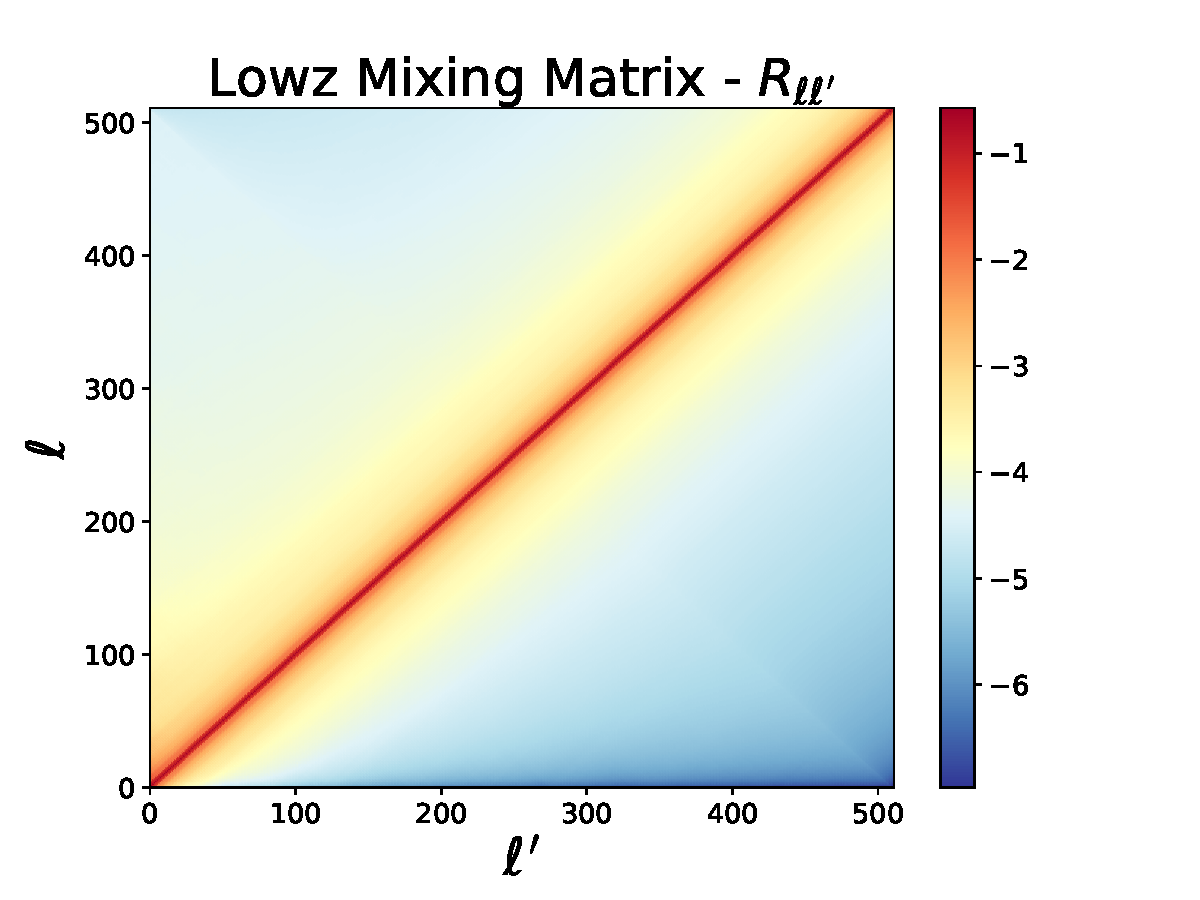
\includegraphics[width=1.2\linewidth]{BOSS-FIGS/MixMat_LOWZ}\label{fig:LOWZ_Rll}
\end{subfigure}%
\begin{subfigure}{.5\textwidth}
  \centering
  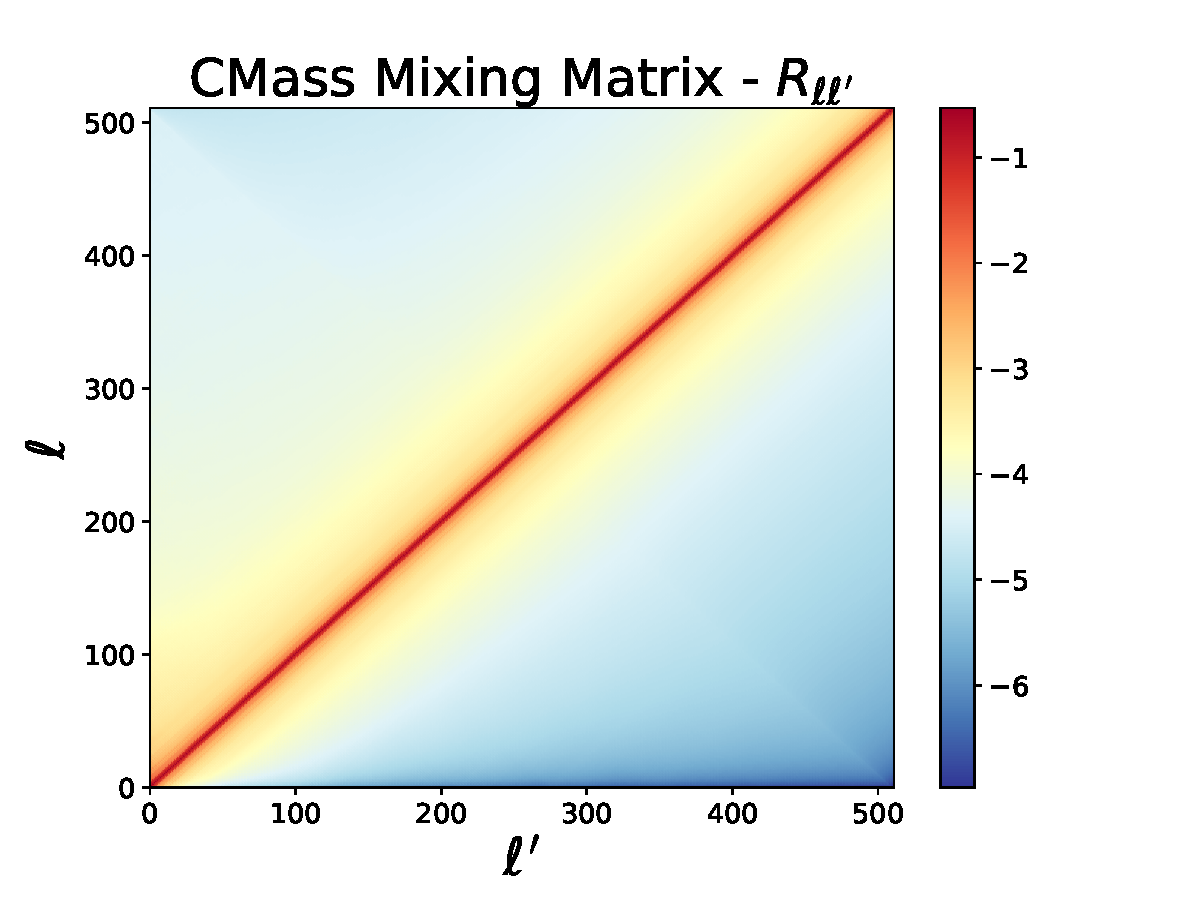
\includegraphics[width=1.2\linewidth]{BOSS-FIGS/MixMat_CMASS}\label{fig:CMASS_Rll}
\end{subfigure}
\caption[Mixing Matrix for CMASS and LOWZ.]{\textit{(left)} Mixing Matrix, $R_{\ell \ell'}$, calculated for the LOWZ mask presented in Fig. \ref{fig:Masks}. \textit{(right)} The Mixing Matrix for the CMASS mask presented in Fig. \ref{fig:Masks}, which is similar to the first one. A closer look on details for both Mixing Matrices can be seen on Fig. \ref{fig:Rll_slice}.}
\label{fig:MixMats}
\end{figure}

\begin{figure}
\begin{center}
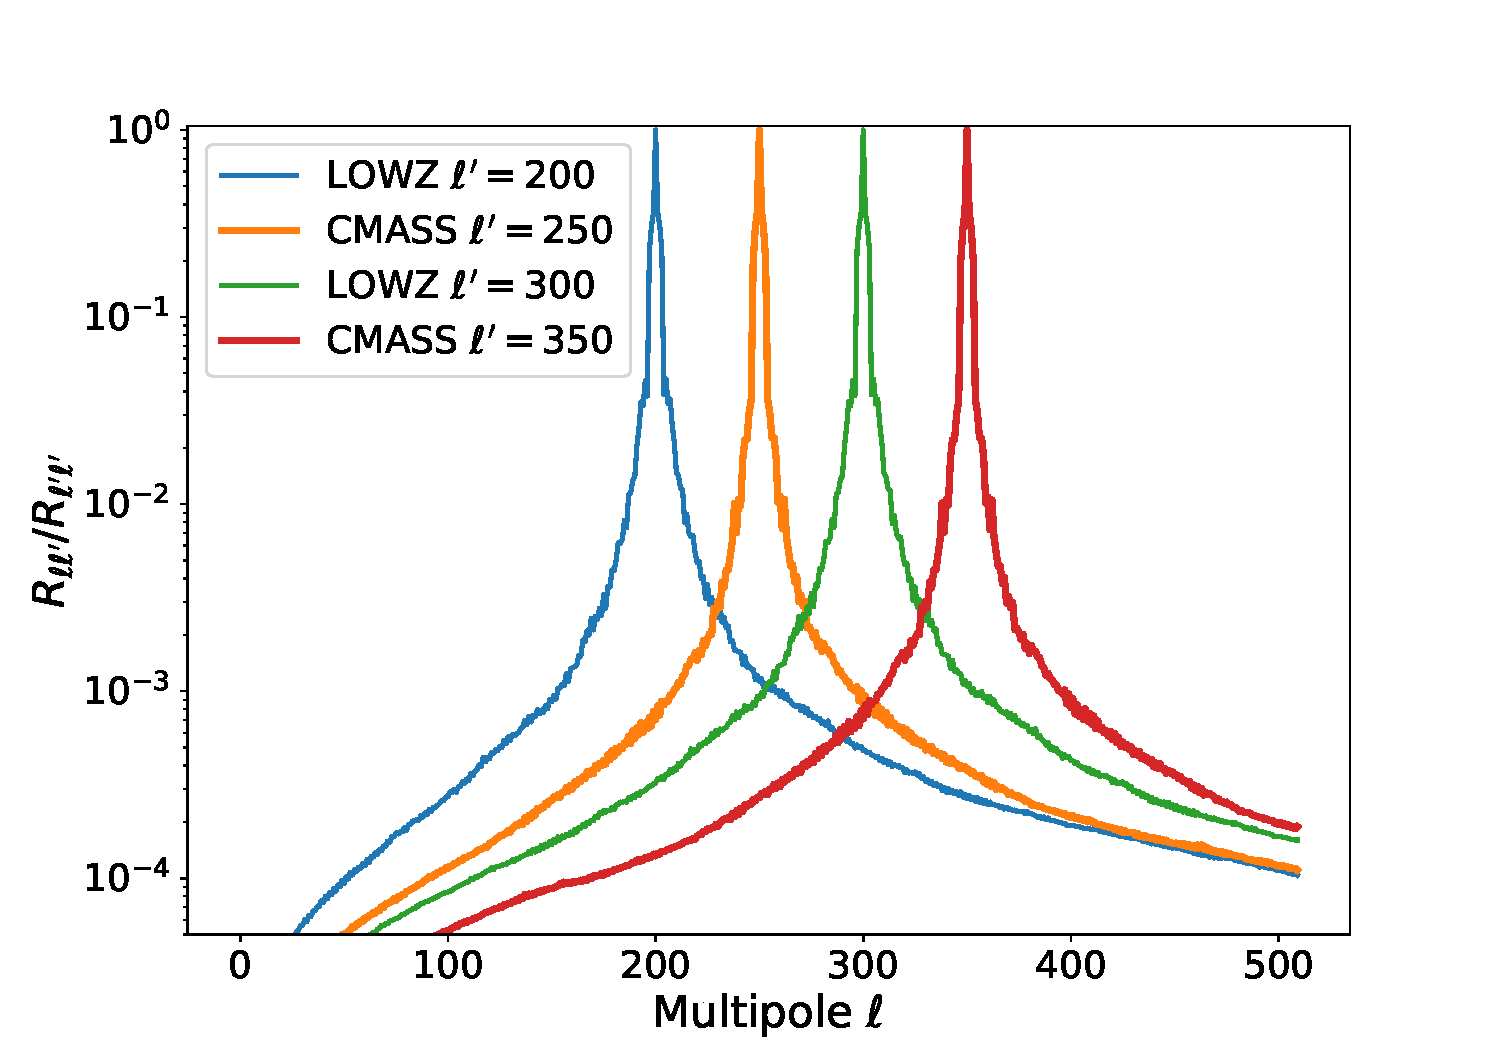
\includegraphics[scale=0.45]{BOSS-FIGS/Rll_200_300.pdf}
\caption[Slices through the Mixing Matrices.]{Slices through the Mixing Matrices (Figs. \ref{fig:MixMats}) for LOWZ (CMASS) using two different fixed multipoles values given by $\ell'=200$($250$), and $\ell'=300$($350$), where the amplitudes were normalized by $R_{\ell\ell}$. As expected, the maximum amplitude peaks in the fixed $\ell'$ and goes to zero in a given $\Delta\ell$. The profile shape of both matrices remains the same throughout the $\ell$-range, indicating the correlation introduced by the convolution with the mask on the PCL measurements presented in Fig. \ref{fig:PCLs}.}
\label{fig:Rll_slice}
\end{center}
\end{figure}

%When dealing with the PCL estimator, I perform a convolution between the theory and the survey's angular selection function effect, due to partial sky observations. As it is computationally expensive to deconvolve this effect from the measurements, this leads us to a forward modelling, where the experimental systematics are modelled and introduced into the theoretical predictions \citep{ScharfLahav1992,FisherLahav1994,Thomas2011}. This effect is taken into account through a convolution with the \textit{mixing matrix}, $R_{\ell \ell'}$ \citep{Peebles1973_2,PolSpice2001,PolSpice2005,Blake2007}:
When dealing the PCL estimator measurements, partial sky effects mean that one must calculate the convolution of the theory and the survey's angular selection function. It is computationally expensive and unstable to deconvolve this effect from the measurements. This leads to forward modelling, where the experimental systematics are modelled and introduced into the theoretical predictions \citep{ScharfLahav1992,FisherLahav1994,Thomas2011}. This effect is taken into account through a convolution with the mixing matrix, $R_{\ell \ell'}$ \citep{Peebles1973_2,PolSpice2001,PolSpice2005,Blake2007}:

\begin{equation}
S_{\ell} = \sum_{\ell'}R_{\ell \ell'} C_{\ell'} \ .
\label{Eq:Cl_Conv}
\end{equation}

\qquad The mixing matrix (see Fig. \ref{fig:Rll_slice}) itself depends only on the survey's geometry through the mask's angular power spectrum
\begin{equation}
W_{\ell} = \sum_{m=-\ell}^{\ell} \frac{|I_{\ell m}|^2}{(2\ell +1)}
\end{equation}
where (from Appendix \ref{Apx:PCL}):
\EQ{Ilm}{ I_{lm} = \sum_p^{N_{pix}} Y_{lm} (\theta_p,\phi_p)\Delta\Omega}
and the mixing matrix can be expressed as:
\begin{equation}
R_{\ell \ell'} = \dfrac{2\ell' + 1}{4\pi}\sum_{\ell ''}(2\ell'' + 1)W_{\ell ''}\begin{pmatrix} \ell & \ell' & \ell'' \\ 0 & 0 & 0 \end{pmatrix}^2.
\label{Eq:MixMat}
\end{equation}

\noindent The $2 \times 3$ matrix above is the Wigner \textit{3j} function; these coefficients were calculated using the \texttt{WIGXJPF} library \citep{Wig3j}. The mixing matrices are shown in Figure \ref{fig:MixMats} and in more detailed slices in Figure \ref{fig:Rll_slice} which gives an intuition about the size of $\Delta\ell$-bands used to bin the \textit{measured} $\hat{S}_{\ell}$s as it shows the range of multipoles that are mixed due to the survey's mask. This small correlations between the multipoles can be ``washed away" by binning the measurements. In addition, as can be seen in Figure \ref{fig:Cl_Theory}, the mixing matrix convolution tends to suppress power in all scales.

\qquad Finally, after being convolved with the mixing matrix (Equation \eqref{Eq:Cl_Conv}), the theoretical $S_{\ell}$ is then binned in the same way as the data in equation \eqref{Eq:S_delta_ell}:
\begin{equation}S_{\Delta\ell}^{ij} = \frac{1}{\sum_{\ell'}^{\ell'+\Delta\ell}(2\ell+1)}\sum_{\ell'}^{\ell'+\Delta\ell}(2\ell+1)S_{\ell}^{ij}  \ .
\label{Eq:S_delta_ell2}
\end{equation}

%------------------------------------------------------------------------%
%                       	 PCL VARIANCE
%------------------------------------------------------------------------%
\subsection{Data Theoretical Covariance}\label{Sec:TheoCov}
Here, I follow the formalism developed in \cite{2008DahlenSimons} for the covariance of spectral estimation on a sphere. For clarity I first re-derive some of the results from Section \ref{Sec:Measurements} from a different perspective, that of projectors in pixel space. 

\qquad Consider a data vector $\textbf{d}$ that is a sum of signal and noise ($\textbf{d}(\textbf{r}) = \textbf{s}(\textbf{r}) + \textbf{n}(\textbf{r})$) and that has a covariance, $\mathcal{D}$, that is a combination of signal covariance $\mathcal{S}$ and a noise covariance $\mathcal{N}$. In pixel space, the data covariance can be expressed as:

\EQ{DataCov}{\mathcal{D} = \langle \textbf{s} \textbf{s}^T \rangle + \langle \textbf{n} \textbf{n}^T\rangle = \sum_{\ell} (S_{\ell} + N_{\ell})\mathcal{P}_{\ell}}
 where $\mathcal{P}_{\ell}$ is the projector in pixel space, defined as:
 
\EQ{Projector}{\mathcal{P}_{\ell} = \sum_{m}Y_{\ell m}(\textbf{r})Y^*_{\ell m}(\textbf{r}).}
The projector satisfies the following identity in the full sky case:

\EQ{ProjIdentFullSky}{tr(\mathcal{P}_{\ell}\mathcal{P}_{\ell'}) = (\Delta\Omega_p)^{-2}(2\ell + 1)\delta_{\ell\ell'}.}
Using this identity, the Pseudo-$C_{\ell}$ estimator from Equation \eqref{Eq:Sl_wl} can be written in terms of the projector and data covariance from \eqref{Eq:DataCov}:

\EQ{}{\hat{S}_{\ell} = \frac{\Delta\Omega_p^2}{(2\ell + 1)}\left[ \textbf{d}^T \mathcal{P}_{\ell}\textbf{d} -tr(\mathcal{N}\mathcal{P}_{\ell})\right].}

\noindent where $\Delta\Omega_p$ is the area the pixels assumed to have an equal area.

\qquad Assuming a Gaussian signal \citep{Blake2007}, the covariance matrix for the angular power spectra estimator between different multipoles $\ell$ and $\ell'$ can be expressed as:

\begin{align}
\Sigma_{\ell \ell'} & = \mathcal{C}ov(\hat{S}_{\ell}, \hat{S}_{\ell'}).
\label{Eq:ThCovSimple}
\end{align}

\qquad The symmetry of the $\mathcal{P}_{\ell}$ and $\mathcal{D}$ matrices, together with the definition $\mathcal{C}ov(\textbf{X},\textbf{X}') = \langle \textbf{XX}'\rangle - \langle \textbf{X}\rangle\langle \textbf{X}'\rangle$, allows us to rewrite the covariance as:

\begin{align}
\Sigma_{\ell \ell'}& = \frac{2(\Delta\Omega_p)^4}{(2\ell+1)(2\ell'+1)}tr(\mathcal{D}\mathcal{P}_{\ell}\mathcal{D}\mathcal{P}_{\ell'})
\label{Eq:CovTrace}
\end{align}

\qquad This expression works for both full and partial sky cases. The difference between the two cases appears on the projector identity from Equation \eqref{Eq:ProjIdentFullSky}. Using the definition of the pixel space projector (Equation \ref{Eq:Projector}), the $I_{\ell m}$ expression from Equation \eqref{Eq:Ilm}, and the fact that the spectra consider in this work are \textit{moderately coloured} \footnote{\textit{Moderately coloured spectra} means that the spectra do not vary drastically within the range considered} \citep{2008DahlenSimons}, one can rewrite Equation \eqref{Eq:ThCovSimple} for a partial sky observation with area $\Delta\Omega_{tot}$ as:

\begin{align}
\Sigma_{\ell \ell'}   = & \frac{1}{2\pi}\left(\frac{4\pi}{\Delta\Omega_{tot}}\right)^2 (S_{\ell} + N_{\ell})(S_{\ell '}+ N_{\ell '}) \times \sum_{\ell ''}(2\ell ''+1)W_{\ell''}\begin{pmatrix} \ell & \ell' & \ell'' \\ 0 & 0 & 0 \end{pmatrix}^2 \\ 
& = \frac{2}{f_{sky}(2\ell' + 1)}(S_{\ell} + N_{\ell})(S_{\ell '}+ N_{\ell '})R_{\ell\ell'}
\label{Eq:CovRll}
\end{align}

where the last equality used the definition of the mixing matrix from Equation \eqref{Eq:MixMat}. Note that this expression is very similar to the one used in \cite{Blake2007,Padm2007,Thomas2011} extending it to account for the mixing of modes due to the mask. 

\qquad However, this expression (derived by \citealt{2008DahlenSimons}) does not account for the pixel window function effect nor for cross-correlations between redshift tomographic bins. In order to include these effects, I need to generalise the data angular power spectra, $S_{\ell} + N_{\ell} \rightarrow w_{\ell}^2S_{\ell}^{ij} + N_{\ell}\delta_{ij} = D^{ij}_{\ell.}$; and include the effect of cross-correlation in the covariance by changing $(S_{\ell} + N_{\ell})(S_{\ell'} + N_{\ell'})\rightarrow \frac{1}{2}[D^{ij}_{\ell}D^{ij}_{\ell'} + D^{ii}_{\ell}D^{jj}_{\ell'}]$ in Equation \eqref{Eq:CovRll} \citep{Rassat2007}. 

\qquad The final expression for the angular power spectra theoretical covariance matrix is:
\begin{align}
\Sigma_{\ell \ell'}^{ij}  = & \frac{1}{f_{sky}(2\ell'+1)}[D^{ij}_{\ell}D^{ij}_{\ell'} + D^{ii}_{\ell}D^{jj}_{\ell'}] R_{\ell \ell'} \\
= & \frac{R_{\ell\ell'}}{f_{sky}(2\ell'+1)} \left[(w_{\ell}^2S_{\ell}^{ij} + N_{\ell}\delta_{ij})(w_{\ell'}^2S_{\ell'}^{ij} + N_{\ell'}\delta_{ij}) \right. \left. + \, (w_{\ell}^2S_{\ell}^{ii} + N_{\ell}\delta_{ii})(w_{\ell'}^2S_{\ell'}^{jj} + N_{\ell'}\delta_{jj}) \right]
\label{Eq:TheoVariance}
\end{align}

and it encompasses for the Gaussian part of the covariance matrix. As in this work I do not use low-$\ell$ modes and scales beyond the non-linear regime, there is no need for further terms to be considered in the theoretical covariance estimation. It is also important to note that this expression is only used to validate the \flask covariances.

\qquad By performing the modifications mentioned above, Equation \eqref{Eq:TheoVariance} recovers the variance expression from \cite{Rassat2007}, when considering just the diagonal, for cross-power spectra; and recovers the original expression by \cite{2008DahlenSimons} when considering just the auto-power spectrum. Figure \ref{fig:Mocks_Variance} shows a comparison between the variance (the diagonal) of equation \eqref{Eq:TheoVariance} with the variance from the estimated covariance matrix from Section \ref{Sec:Cov}. Note that the covariance between different angular power spectra is considered to be zero, i. e. $\Sigma^{ij,i'j'}_{\ell\ell'} = \Sigma^{ij}_{\ell\ell'} \delta_{ii'}\delta_{jj'}$.

\begin{figure}
\begin{center}
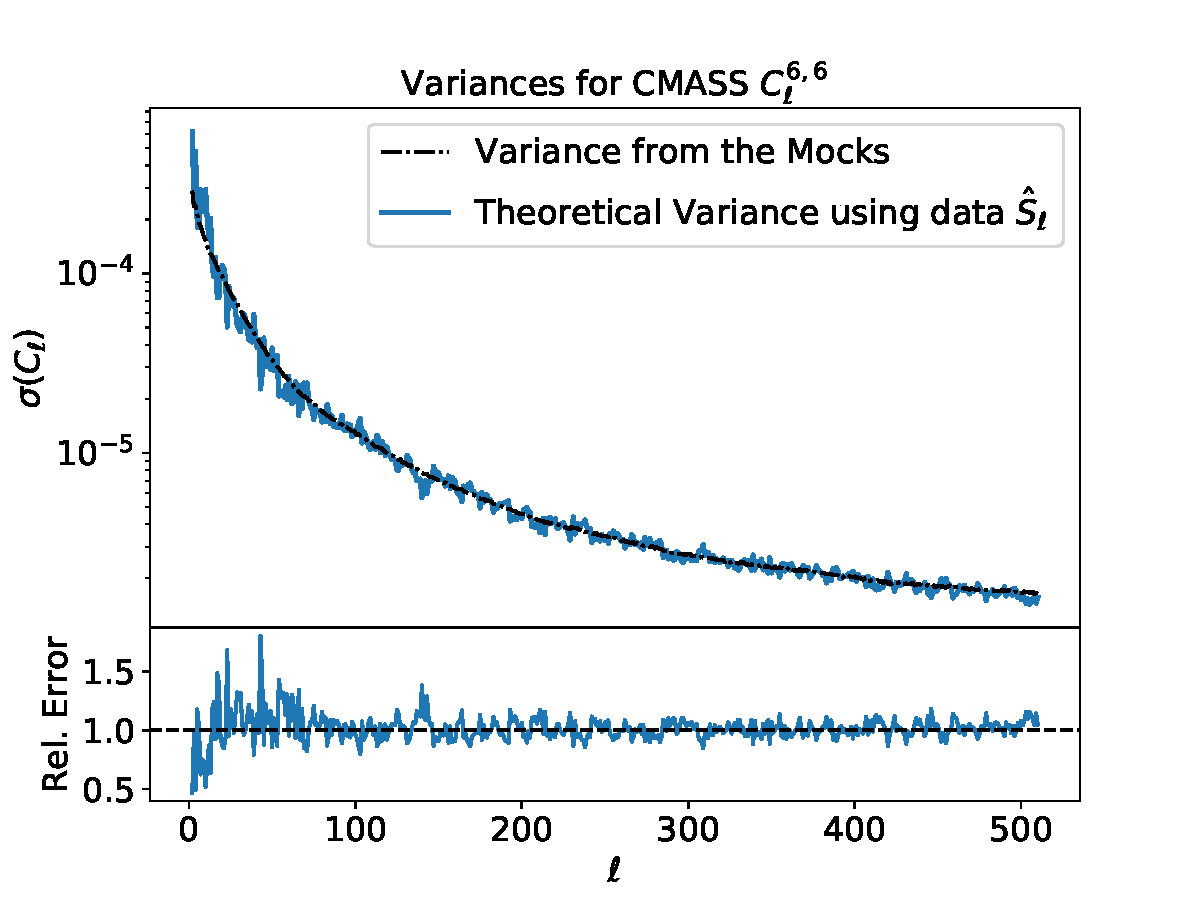
\includegraphics[scale=0.55]{BOSS-FIGS/MocksValidation.pdf}
\caption[Mock's covariance matrix validation.]{An example used for the mock's covariance matrix validation: here I compare the analytical expression for the angular power spectrum variance (Equation \eqref{Eq:TheoVariance}) with the variance from the log-normal mocks using CMASS' first auto-power spectrum as an example. The bottom panel shows the relative error for this case. This validation was checked for each one of the 42 measured $C_{\ell}$'s from fig. \ref{fig:PCLs} and no trends are apparent.}
\label{fig:Mocks_Variance}
\end{center}
\end{figure}

\subsection{Covariance Matrix using log-normal Mocks}\label{Sec:Cov}
%When obtaining cosmological parameters constrains from the PCL measurements presented in Section \ref{sec:BOSS:Measurements}, one needs reliable covariance matrices in order to estimate the measurement's errors. These covariances can be estimated using galaxy clustering mocks which reflect the cosmology, systematics effects, and any possible observational artifices that can influence the data. To do so, I use log-normal simulations instead of using Gaussian realisations \citep{Blake2007, Thomas2011} or the mocks provided by the BOSS Collaboration \citep{2016BOSSMocks}. One of the reasons why I do not make use of the official BOSS \texttt{PATCHY} mocks from \cite{2016BOSSMocks} is due to the different choice of redshift ranges for the samples: the CMASS \texttt{PATCHY} mocks do not contain galaxies beyond redshift $z_{max} \leq 0.75$ as the samples I selected go beyond this redshift range with $z_{max} \leq 0.80$ (Section \ref{sec:BOSS:data}). 
As I seek to constrain cosmological parameters using observations; one of the requirements of this process is accurate covariance matrices. Covariances can be estimated using galaxy clustering simulations that reflect not only the cosmology but also systematic effects and observational artefacts. Previous works have used either Gaussian realisations \citep{Blake2007,Thomas2011,2016Nicola} or the mocks provided by the BOSS Collaboration \citep{2016BOSSMocks,Manera2013}. However this work instead uses log-normal simulations. The decision not to use the official BOSS \texttt{PATCHY} mocks from \cite{2016BOSSMocks} was made due to the different choice of redshift ranges for the samples: the CMASS \texttt{PATCHY} mocks do not contain galaxies beyond redshift $z = 0.75$ whereas the samples I selected extend to $z = 0.80$ (as described in Section \ref{Sec:Data}). 

% \begin{figure}
% \begin{subfigure}{.5\textwidth}
%   \centering
%   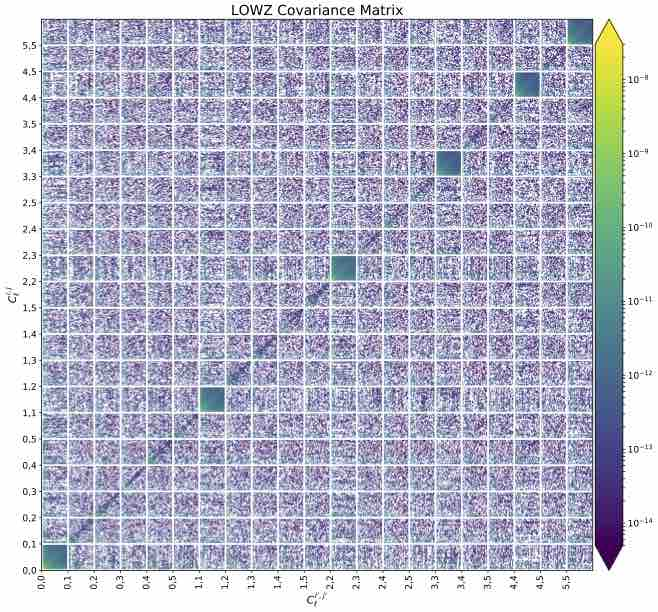
\includegraphics[width=1.\linewidth]{BOSS-FIGS/LOWZ_COV_Temp_TUAMAE.jpg}\label{fig:LOWZ_COV_Temp_TUAMAE.jpg}
% \end{subfigure}%
% \begin{subfigure}{.5\textwidth}
%   \centering
%   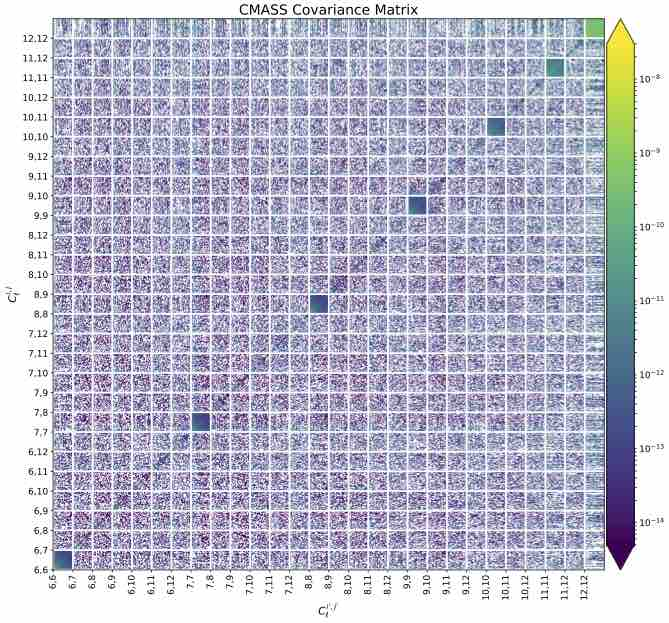
\includegraphics[width=1.0\linewidth]{BOSS-FIGS/CMASS_COV_Temp_TUAMAE.jpg}\label{fig:CMASS_COV_Temp_TUAMAE.jpg}
% \end{subfigure}
% \caption{Covariance matrices created with 6,000 \texttt{FLASK} log-normal simulations for \textit{(left)} LOWZ and  \textit{(right)} CMASS. The labels on the axis are the number (\textit{i,j}) of the redshift bins for covariance $\mathcal{C}(\hat{S}_{\Delta\ell}^{i,j},\hat{S}_{\Delta\ell'}^{i',j'})$.}
% \label{fig:CovMat}
% \end{figure}

\qquad To generate the mocks, I use \texttt{FLASK}\footnote{\url{http://www.astro.iag.usp.br/~flask/}} \citep{Flask2016}, a publicly available code that produces log-normal simulations of correlated fields in the sphere. Here, I use the data $\hat{S}_{\ell}$ measurements as inputs for the simulations (as measured in Section \ref{Sec:Measurements}). This technique allows me to reproduce any sort of systematic effects, RSD, non-linear power spectra, and other known and unknown effects that may be present in the data with no need to model them nor assume any fiducial cosmology. This is a main benefit of this approach to covariance estimation: any effects present in the measured angular power spectra will be reproduced in \texttt{FLASK}'s simulations via the $S_{\ell}$s measured from the data. 

\qquad For each of the samples, I produced 6,000 log-normal mocks to estimate the data covariance matrix. These mocks are also Poisson sampled to reproduce noise properties, radial and angular selection effects according to the data. 

\qquad The data covariance matrix was produced as follows:

\begin{enumerate}
\item[\textbf{1.}] Produce an spline, $\tilde{S}(\ell)$, using the $\hat{S}_{\Delta\ell}$ measurements (Figure \ref{fig:PCLs}) and a Gaussian filter to smooth the measurements.
\item[\textbf{2.}] Deconvolve the mixing matrix, $R_{\ell\ell'}$, from the splines to obtain
\begin{align}
\tilde{C}^{ij}(\ell) = \sum_{\ell'}R_{\ell\ell'}^{-1}\tilde{S}^{ij}(\ell)
%\label{Eq:Spline}
\end{align}
\item[\textbf{3.}] Monotonically extrapolate the splines to $\ell_{max} = 8192$ (necessary to allow \texttt{FLASK} to create high resolution \healpix maps).
\item[\textbf{4.}] For each tomographic redshift bin, produce \texttt{FLASK} partial sky galaxy number count mocks with $N_{side} = \ell_{max} = 2048$.\footnote{The signal realisation maps were sampled using a log-normal transformation. Due to the transformation's non-linearity, I had to generate mocks with a higher $N_{side} \quad \& \quad\ell_{max}$ than the data as the log-normal realisations introduce a damping after a certain $\ell$ (see figure 18 from \cite{Flask2016}). The simulated data maps also used a $N_{side}=2048$ version of the masks presented in \ref{Sec:Masks}.}
\item[\textbf{5.}] Degrade the mocks to $N_{side}=512$ to match the $N_{side}$ used when analysing the data.
\item[\textbf{6.}] Produce up-weighted overdensity maps (as described in section \ref{Sec:Maps}).
\item[\textbf{7.}]Run the partial sky PCL estimator; include here the pixel window function correction $w_{\ell}^2$ (as described in Equations \eqref{Eq:Sl_wl} and \eqref{Eq:S_delta_ell}) that arises from the degrading of the maps at step \textbf{5}.
\item[\textbf{8.}] Measure the covariance of the ensemble of angular power spectra obtained from the simulated data:
\begin{equation}
\mathcal{C}^{ij}_{\Delta\ell\Delta\ell'} \equiv \frac{1}{N_S-1}\sum^{N_S}_{s=1}\left(S_{\Delta\ell}^{ij,s} - \langle S_{\Delta\ell}^{ij} \rangle \right)\left(S_{\Delta\ell'}^{ij,s} - \langle S_{\Delta\ell'}^{ij} \rangle \right)^T.
\label{Eq:Covariance}
\end{equation}
\end{enumerate}
Here $N_S$ is the number of simulations.
To validate the estimated covariance matrix, I compared the diagonal of the covariance matrix in Equation \eqref{Eq:Covariance} with the expression for the theoretical variance for the measured angular power spectra in Equation \eqref{Eq:TheoVariance}; Figure \ref{fig:Mocks_Variance} shows a typical result.

\section{Systematic Null Tests}\label{Sec:Systm}
Large-scale survey observations, spread over thousands of observation hours, are taken under a variety of conditions. Turbulence in the atmosphere, sky background brightness and telescope inclination angle are amongst the factors that can influence image quality and object detection. Other than those atmospheric effects, galactic properties are also at play: extinction from dust within the Milky Way and variations of stellar density, as well as the presence of bright stars, are position-dependant and also have an impact on our ability to detect galaxies. Jointly, these observational factors have the potential to create small density fluctuations in the galaxy distribution which can imprint a statistical signal easily confused with the cosmological large-scale structure fluctuations that one is attempting to measure. This effect has been detected and corrected for in several previous analyses with a range of datasets \citep{Blake2007, 2011MNRAS.417.1350R, Thomas2011, Boris2013, Ho2012, Doux2017}.

\qquad In this section, I present the analysis performed on the data to ensure that the measured power spectra are not significantly dominated by any known observational systematic effects. I consider a systematic to have a significant effect on the observed power spectra if the cross-power spectra between them deviates from zero, with a deviation that is bigger than both the data variance and the cross-power spectra variance. I start by describing the systematic effects considered in this analysis, describing the methods for map creation and cross-spectrum measurement, and giving some representative results. Plots showing the complete analysis of systematics contamination for all 13 tomographic bins can be found in Appendix \ref{Apx:Systematics}.

%------------------------------------------------------------------------%
%                        	SYSTEMATICS MAPS
%------------------------------------------------------------------------%
\subsection{Systematic Maps}\label{Sec:SystMaps}

The Sloan Digital Sky Survey monitors and records observational conditions for every tile of the survey. This information is available as a combined set of two files, one that defines a pixelisation of the observed sky in \mangle format and another that records the observational information for each \mangle polygon.\footnote{The files, \texttt{window\textunderscore unified.fits} and \texttt{window\textunderscore flist.fits}, can be found in \url{http://www.sdss.org/dr12/algorithms/resolve/}, together with a detailed description of the construction of the survey geometry and of the \texttt{score} quantity described further in the text.} The first step is to reconstruct the \mangle maps for each observational systematic from these files. The \mangle python wrapper\footnote{\url{https://github.com/mollyswanson/manglepy}} was used to perform this transformation. Since there is potentially more than one observation in a given region of the sky, there can be multiple values for a given polygon. The SDSS files indicate which amongst multiple options is to be taken as the primary value for the field. The IDs were selected from those primary fields, matched to their observational properties in the fields list, and a new \mangle mask was created for each of those properties, which are recorded in the weight of the masks.

\qquad Next, \texttt{Mangle} masks were created for sky background flux, sky variance and average PSF FWHM in all five photometric bands. Mask of the \textit{score} of each field were also created -- defined by the SDSS collaboration to express ``observational quality" as an empirical combination of observational values with processing status flags. Additional observational properties can be found in the Field Table, available from the SDSS SkyServer Schema Browser.\footnote{\url{http://skyserver.sdss.org/dr12/en/help/browser/browser.aspx}} The choice of which systematics to take into account is somewhat arbitrary, as there are correlations between observational properties that make information redundant \citep{Boris2013}. Stellar density and galactic extinction were also added to the systematics listed above, as those have been shown to correlate with galaxy density in several previous analyses \citep[e.g.][]{Thomas2011, ElvinPoole2017}.The bright star catalogue was created from the SDSS object catalogue with the following cuts:
\begin{eqnarray}
18 < r_{psf} < 19.5,\\ \nonumber
\text{type} = 6,\\
r_{psf} - r_{\text{model}} < 0.25,\nonumber
\end{eqnarray}
where the extinction-corrected magnitude cut ensures robust star selection \citep{Padm2007}, the type selection is the standard SDSS star-galaxy classifier\footnote{\url{http://www.sdss.org/dr12/algorithms/classify/}} and the magnitude-difference cut is an additional point-source selection performed by the \texttt{GAMA} survey \citep[e.g.][]{Christodoulou2012}. For galactic extinction, a \healpix map was created directly. For simplicity, a python implementation of extinction $E(B-V)$ value retrieval and map creation\footnote{\url{https://github.com/kbarbary/sfdmap}} was used to create such map. Finally, the original SFD scaling map \citep{Schlegel1998} was also used.

\qquad The \mangle masks created from the SDSS FITS files are not appropriately snapped, pixelised and balkanised, which breaks the local character of the \mangle procedure \citep{2008Mangle}. As a consequence, further operations suffer from impractically large processing times. All the steps of the \mangle pixelisation scheme were ran anew, which corrects whatever imperfections remained in the first pass. From these masks, full-sky \healpix maps at resolution $N_{side}=16384$ were created, which defines an angular scale much smaller than the average resolution of the mask features. For each observational systematic, the sub-resolution \healpix pixels were populated with values from the associated \mangle mask. The resulting \healpix maps encapsulate all the information contained in the original footprint description.

\qquad Once the \healpix systematics maps are created, the next step is to transform them into overdensity maps using the same procedure outlined in Section \ref{Sec:Maps} for the data \citep{Boris2013}. The idea is to treat the systematic maps in the same way as the data in order to apply the statistical estimators consistently. Therefore, I degrade the high-resolution maps to the data resolution ($N_{side} = 512$) and up-weight the maps according to the pixel completeness mask that takes the holes in the footprint into account (see Section \ref{Sec:Masks}); I then perform a cut in pixel completeness $C_{pix} = 0.8$ in the maps. From these post-processed maps, I create the systematics overdensity maps as: 
\begin{equation}
\delta_{i}^{Sys} = 
\begin{cases}
\left(\frac{1}{C_{pix,i}}\frac{n^{Sys}_{i}}{\bar{n}^{Sys}}\right) - 1 & \text{, if } C_{pix,i} \geq 0.8 \\
0 & \text{, otherwise}
\end{cases}
\label{Eq:OverDMapsSyst}
\end{equation}
where $n^{Sys}_{i}$ is the pixel value for a given systematic and $\bar{n}^{Sys}$ is the mean value of the map in the observed fraction of the sky. The systematics overdensity maps were created using both the CMASS and LOWZ masks presented in Section \ref{Sec:Masks}. The resulting systematics overdensity maps are shown in figure \ref{fig:SYS_Appendix1Map} and in figure \ref{fig:ExtincSys} for extinction using the CMASS mask as an example.

\begin{figure}
\begin{center}
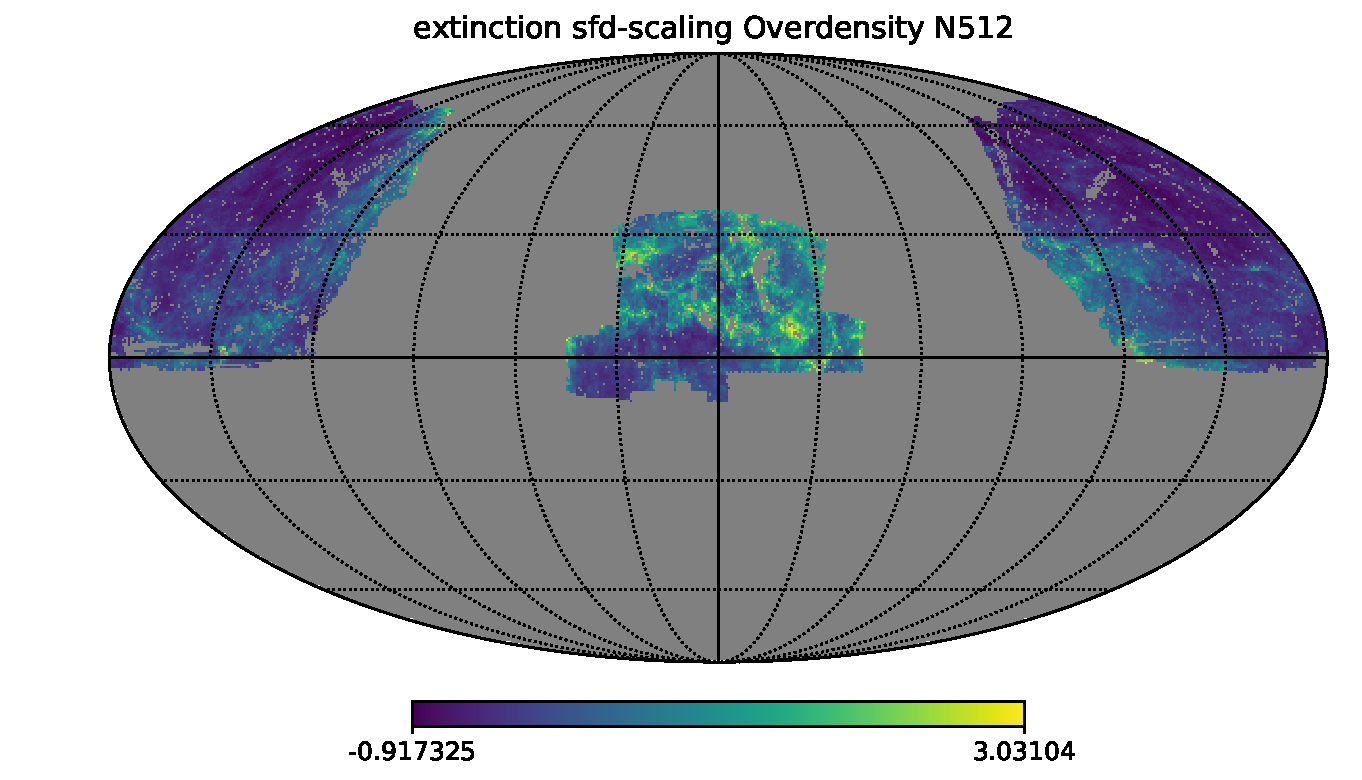
\includegraphics[width=\textwidth]{BOSS-FIGS/map_extinction_sfd-scaling_Overdensity_N512_cmassAll.pdf}
\caption[Extinction SDF scaling overdensity systematic map.]{An example of systematics overdensity maps from Section \ref{Sec:SystMaps}: the extinction sfd scaling map \citep{Schlegel1998} using the CMASS mask from Section\ref{fig:Masks}. }
\label{fig:ExtincSys}
\end{center}
\end{figure}

%------------------------------------------------------------------------%
%                        	SYSTEMATICS CROSS-CLS
%------------------------------------------------------------------------%
\subsection{Cross-power spectra between data and systematic maps:}\label{Sec:SystCls}
\begin{figure*}
\begin{center}
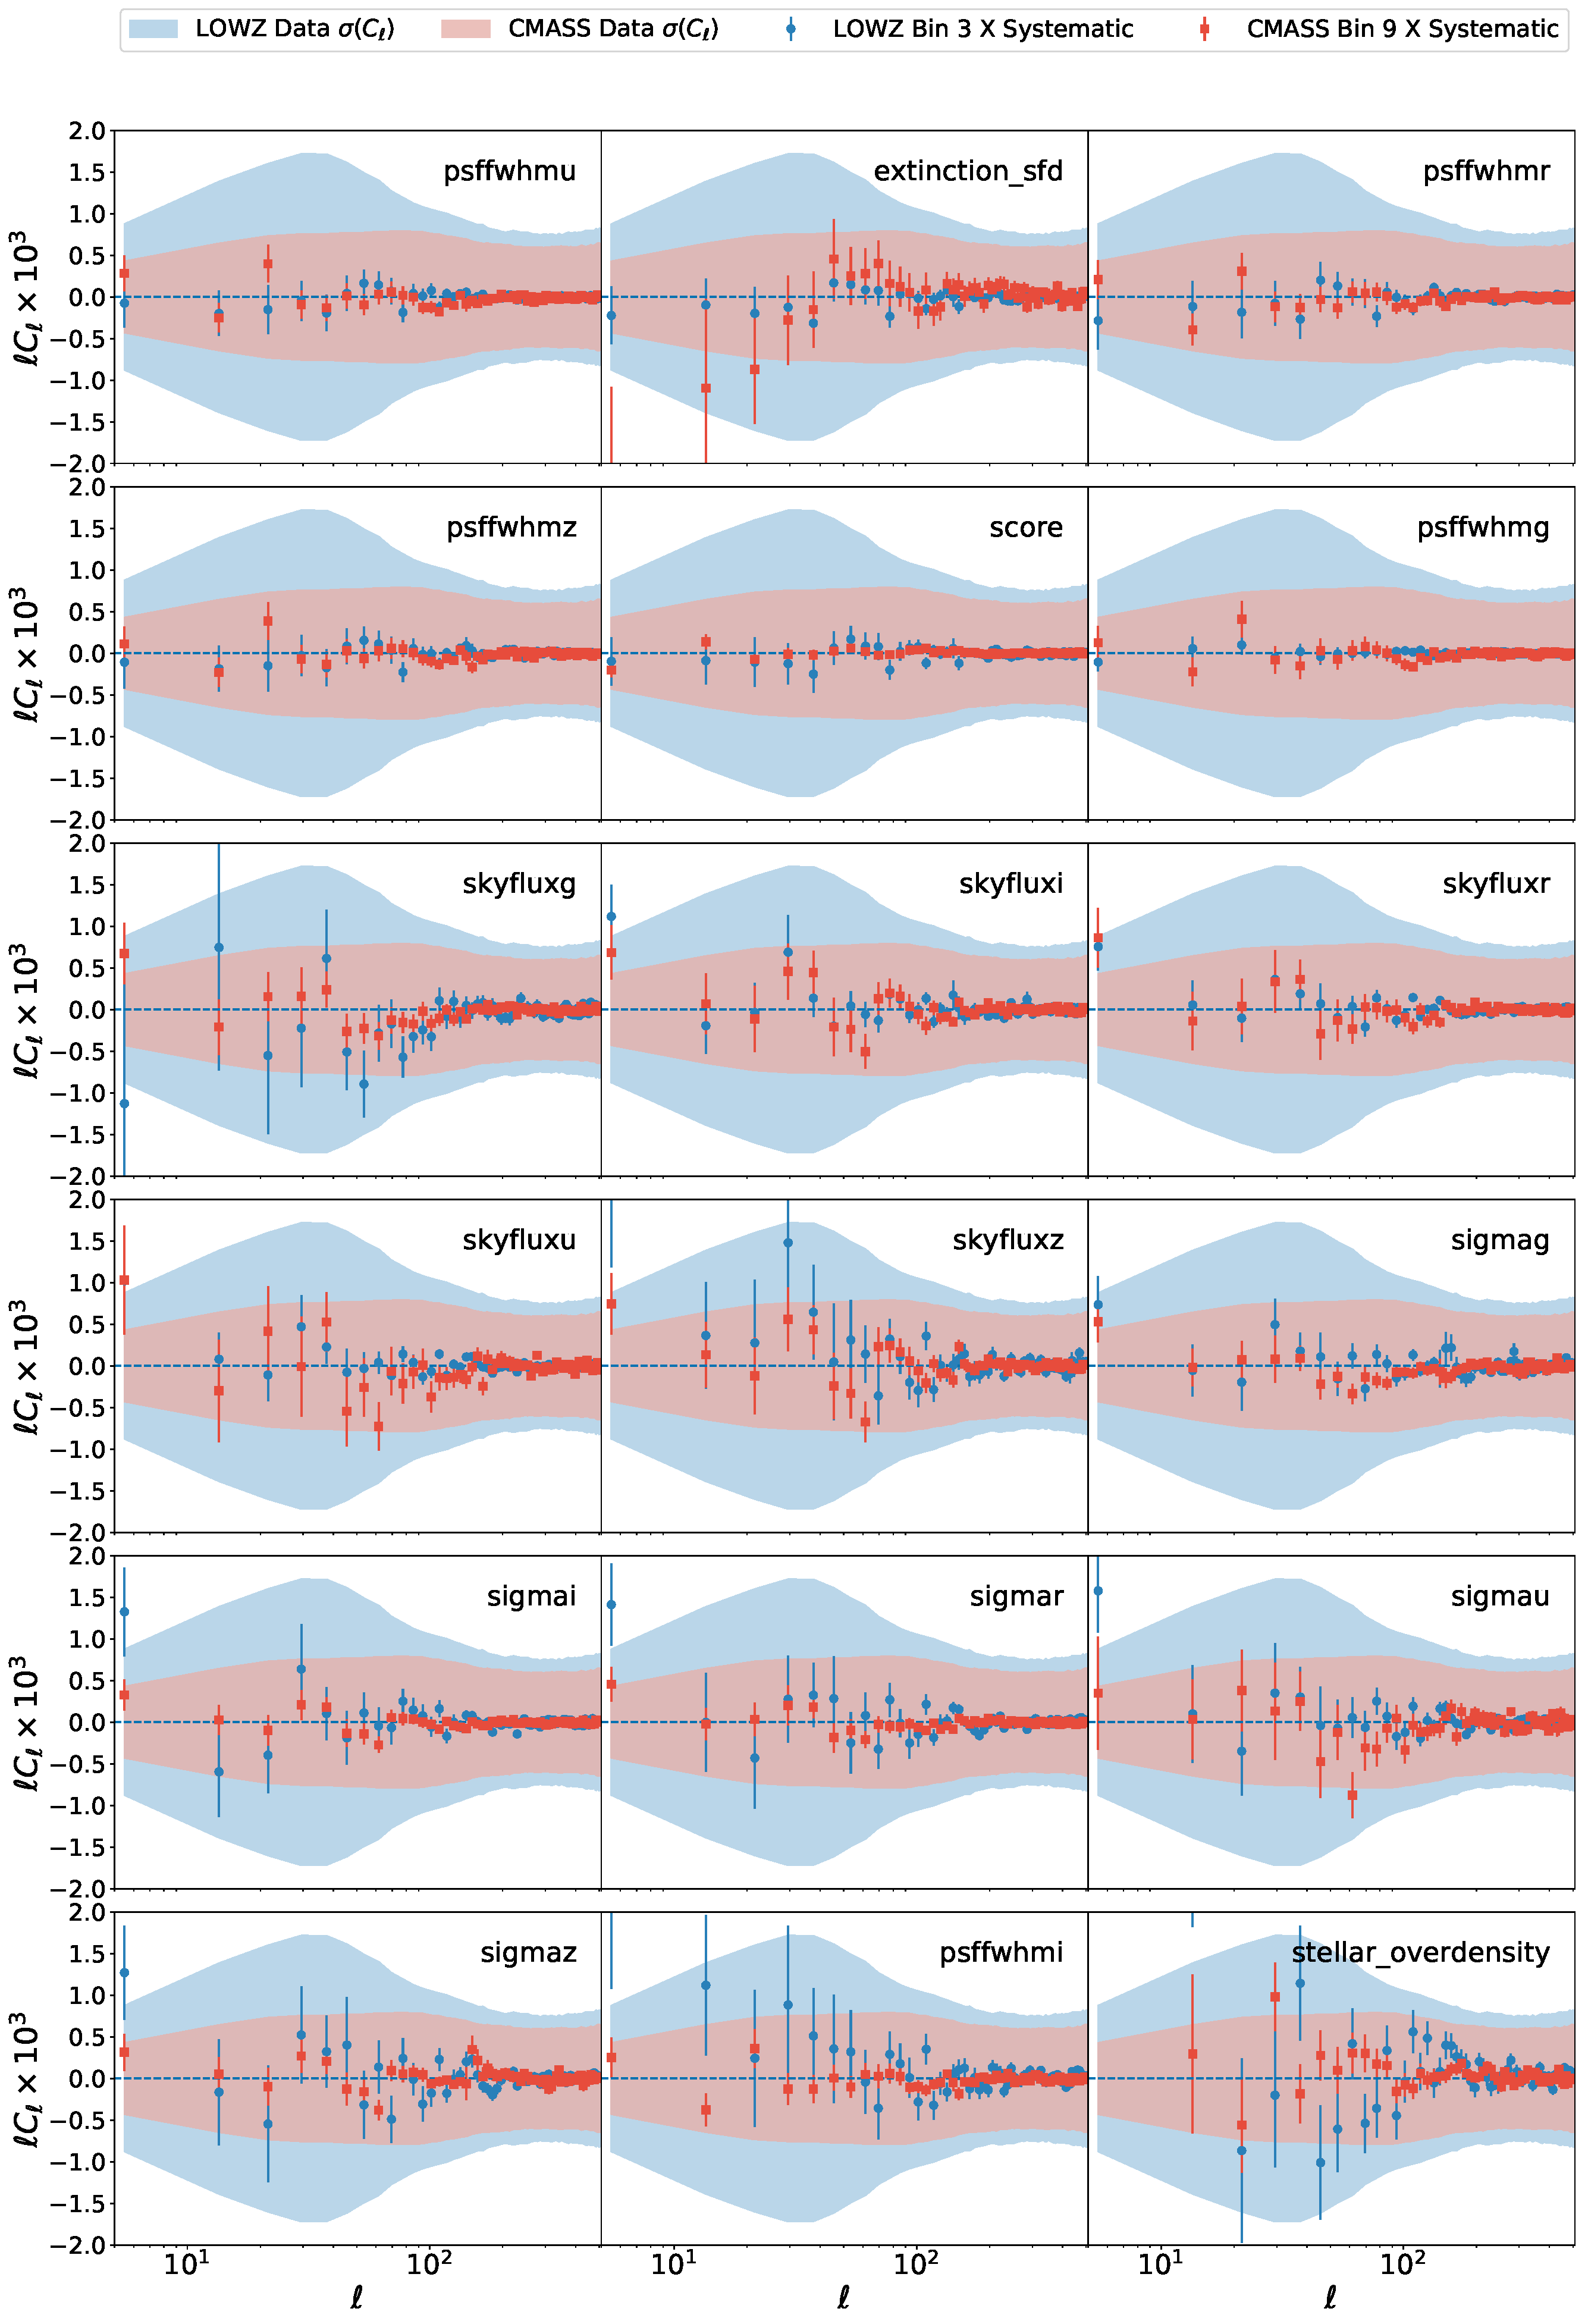
\includegraphics[scale=0.30]{BOSS-FIGS/systematics_CMASS_Bin3_LOWZ_Bin3.pdf}
\caption[An example of the systematics analysis for the BOSS samples.]{An example of the systematics analysis described in Section \ref{Sec:SystCls}. Here, I show the cross-power spectra between the 18 systematics overdensity maps produced in \ref{Sec:SystMaps}, and LOWZ--3 (CMASS--9) tomographic bins in blue dots (red squares). The error-bars were obtained by cross-correlating the $\delta^{Sys}$ maps with the \texttt{FLASK} mocks produced in Section \ref{Sec:Cov}; the shaded region shows the variance of the data, which was also obtained from the same mocks. This figure indicates that the shape of the measured power spectra in Figure \ref{fig:PCLs} is not dominated by any of the systematics considered, as the variance of the cross-power spectra between data and systematics is consistent with the variance of the data's auto-power spectra. The results for the other bins similar to the results shown in this figure and can be found in Appendix \ref{Apx:Systematics}. Note also that the first $\ell-$band in the stellar overdensity cross-$C_{\ell}$ is completely out of the acceptable range, which lead me to exclude this data point on all bins for both samples.}
\label{fig:SystBin3}
\end{center}
\end{figure*}
For the systematics analysis using cross-power spectra, I follow a data analysis in a similar fashion as the one performed for the galaxy overdensity maps in Section \ref{Sec:Measurements}.  Using Equation \eqref{Eq:AlmPix} I decompose the systematics overdensity maps, $\delta^{Sys}$, into spherical harmonics. 

The estimator for the cross-power spectra between the data overdensity maps, $\delta^{g}$, and the systematics can be written as a modified version of Equation \eqref{Eq:Sl_wl}:

\begin{equation}
\hat{S}^{gs}_{\ell} = \frac{1}{(2\ell+1)w_{\ell}^2}\sum_{m=-l}^l  \frac{\frac{1}{2}\left|d_{}^{g}  d_{\ell m}^{s*} + d_{\ell m}^{g*}  d_{\ell m}^{s}\right|}{J_{\ell m}}
\label{Eq:Sl_wlSyst}
\end{equation}
where the index \textit{g} stands for a data map, and \textit{s} for a systematics map. I then obtain the estimates for the variance of the systematics cross-power spectra by measuring the $\hat{S}^{gs}_{\ell}$ (Equation \eqref{Eq:Sl_wlSyst}) between the Systematics maps and the data mocks described in Section \ref{Sec:Cov}.

\qquad I cross-correlated all 13 tomographic redshift bins with all 18 systematic maps, resulting in a total of 234 cross-power spectra. Figure \ref{fig:SystBin3} shows an example for LOWZ--3 and CMASS--9 bins and cross-power spectra for all systematics. The full results are shown in Appendix \ref{Apx:Systematics}. From all of these, the majority of measurements are consistent with the variance of the data measured from the log-normal simulation (Section \ref{Sec:Cov}), which lead me to be confident in using the full shape of the measured $C_{\ell}$s. Note, however, that a few of the large scale measurements (low-$\ell$) in CMASS sample have a small excess in cross-power spectra with stellar overdensity. The first point on the cross-power spectra between some of the systematic maps and most BOSS bins is clearly more than one sigma away from the data's variance. Due to this excess in correlation with stellar overdensity and the level of cosmic variance on the first $\ell$-band, I decided to exclude this first point from the cosmological analysis (see Chapter \ref{Chap:BOSS-Cosmo} for details on the $\ell$ range used). As for the second $\ell$-band ($\ell = 13.5$) presenting an excess of correlation between a few bins and stellar overdensity: I found it to be sub-dominant, with no significant impact from this measurement in our cosmological analysis; therefore, I decided to keep it.

\section{Conclusions}\label{Sec:Concl1}
%In this chapter, I presented the process towards building a full data-vector for the BOSS DR12 large scale structure sample using a harmonic space approach. Given the spectroscopic nature of the data-set, I was able to divide it into 13 redshift tomographic bins with an equal size ($\Delta z = 0.05$). This
In this work, I have taken a different approach\footnote{Compared to the approaches from the official BOSS Collaboration papers: \cite{2017RossBOSS,2017BeutlerBOSS,2017Beutler2BOSS,2017SatpathyBOSS,2017SanchezBOSS,2017GriebBOSS,2017SalazarBOSSwTheta,2017WangBOSS,2017ZhaoBOSS}.} to obtain galaxy clustering information from the BOSS DR12 large scale structure catalogue \citep{BOSSCatalogue2016}. This approach consisted in using a pseudo angular power spectra estimator (PCL) applied to 13 tomographic redshift bins ranging from $0.15 \leq z < 0.8$ with a redshift dependent bias, a redshift dispersion, and extra shot-noise as nuisance parameters to be sampled with the cosmological parameters using \uclcl (Cuceu et al., \textit{in prep}). In this approach, I have used splines of the data as input for the simulation used for covariance matrix estimation.

\qquad The tomographic analysis in redshift space and the covariance matrix estimation method used in this work allow for cosmology-free inference to be performed from the data. In other words, in no moment in this analysis a fiducial cosmology was assumed. This is, by itself, a great advantage over methods that use $P(k)$ or $\xi(r)$ as these need to assume a fiducial cosmology in order to transform from redshift space to radial distances. The impact of such strong assumption in the cosmological inference is still unknown.

\qquad I performed systematic contamination checks with the data with satisfactory results. From the 18 different sources of systematic considered in Section \ref{Sec:Systm}, none demonstrated worrying excess of power in the scales considered (with the exception of the first bandwidth, $\Delta \ell = [2,10]$). Although some other $\ell$-modes do present a small excess of clustering with, for example, stellar overdensity, these were not found to have a significant impact on the overall clustering of galaxies when compared to the intrinsic variance of the data -- estimated from the log-normal simulations.

\qquad Finally, I have constructed a data-vector and covariance matrices from a spherical harmonic analysis of BOSS DR12 galaxies which are cosmology-free, i.e. no fiducial model was assumed at any moment in this analysis. With the theoretical framework detailed in Section \ref{Sec:Theory}, these measurements are now ready to be used in a cosmological posterior analysis to infer cosmological parameters. The next Chapter performs some additional checks in the methodology and data-vector outlined here; subsequently probing the main cosmological models and demonstrating the full constraining power of the data-vector produced in this Chapter. % INCLUDE: related work
% !TEX root = ../thesis-example.tex
%
%\chapter{Cosmological Measurements from Angular Power Spectra analysis of BOSS DR12 Tomography}
\chapter{Cosmological Measurements from Angular Power Spectra Analysis of BOSS DR12 Tomography}
\label{Chap:BOSS-Cosmo}

\cleanchapterquote{The truth knocks on the door and you say, "Go away, I'm looking for the truth," and so it goes away. Puzzling.}{Robert M. Pirsig}{(Zen and the Art of Motorcycle Maintenance)}
\vspace*{\fill}

In this chapter, I constrain cosmological parameters by analysing the angular power spectra of the Baryon Oscillation Spectroscopic Survey DR12 galaxies. Sanity and consistency checks are performed in the analysis pipelines, the data-vector and covariances, and in the data itself. Cosmological constraints obtained from these measurements were combined with constraints from Planck CMB experiment as well as the JLA supernovae compilation. Considering a $w$CDM cosmological model measured on scales up to $k_{max} = 0.07h$ Mpc$^{-1}$, I constrain a constant dark energy equation-of-state with a $\sim 4\%$ error at the 1-$\sigma$ level: $w_0 = -0.993^{+0.046}_{-0.043}$, together with $\Omega_m = 0.330\pm 0.012$, $\Omega_b = 0.0505 \pm 0.002$, $S_8 \equiv \sigma_8 \sqrt{\Omega_m/0.3} = 0.863 \pm 0.016$, and $h = 0.661 \pm 0.012$. For the same combination of datasets, but now considering a $\Lambda$CDM model with massive neutrinos and the same scale cut, I find: $\Omega_m = 0.328 \pm 0.009$, $\Omega_b = 0.05017^{+0.0009}_{-0.0008}$, $S_8 = 0.862 \pm 0.017$, and $h = 0.663^{+0.006}_{-0.007}$ and a 95\% credible interval (CI) upper limit of $\sum m_{\nu} < 0.14$ eV for a normal hierarchy. These results are competitive if not better than standard analyses with the same dataset, and demonstrate this should be a method of choice for future surveys, opening the door for their full exploitation in cross-correlations probes.

\textit{The work presented in this chapter was presented in \citet{2018LoureiroBOSS}.} 
\newpage
%------------------------------------------------------------------------%
%                        COSMOLOGICAL BANANAS
%------------------------------------------------------------------------%
%\section{Cosmological Analysis}\label{Sec:CosmoBananas}
\section{Introduction}
For over 20 years, the current cosmological paradigm, the $\Lambda$CDM model, is the most intriguing mystery modern cosmologists are collectively trying to solve. For an extremely simple model -- containing only six free parameters -- the current scenario fails to explain the nature of two of the most important characteristics of this scenario: dark energy and cold dark matter. If warm, dark matter could be easily explained by the energy density of cosmic neutrinos; however, since neutrinos, even having non-zero mass, are relativistic the effect they have is the opposite of cold dark matter: they then to wash away structure instead of amplifying the clustering of matter. From the other perspective, the simplest approach to study dark energy is to parametrize it via its equation-of-state parameter, $w_0$. The hopes are that, if measured with sufficient accuracy and precision, $w_0$ could give us hints on what could be the possible nature of such strange component in our Universe. However, if $w_0 = -1$, we continue to fall under the $\Lambda$CDM scenario since dark energy is then better described to be simply the mysterious cosmological constant postulated by \cite{1917Einstein}. State-of-the-art cosmological surveys such as Planck \citep{PlanckCosmology2016,2018PlanckCosmology} and the Dark Energy Survey \citep{2017arXiv170801530D,2018DES-SNe} measure the equation-of-state of dark energy with percent level precision to be that of a cosmological constant case.

\qquad In this Chapter, I present the cosmological implications from the measured angular power spectra of BOSS galaxies (see Chapter \ref{Chap:BOSS}) for flat $\Lambda$CDM, $w$CDM, and a $\Lambda$CDM with $\sum m_{\nu}$ models. Using the theoretical framework and having estimated covariance matrices as described in Section \ref{Sec:Theory}, I performed a Bayesian analysis using the \texttt{PLINY} nested sampler ( \citealt{PlinyRichardThesis} and Rollins et al., \textit{in prep}) and the \textit{Unified Cosmological Library for Parameter Inference} code, or \texttt{UCLPI} (Cuceu et al., \textit{in prep.}). All analyses considered in this section use the auto-power spectra and the cross-power spectra from adjacent tomographic bins -- the measurements presented in Section \ref{Sec:Measurements}. Cross-power spectra between distant bins are not a part of the final BOSS-$C_{\ell}$ data vector.

\qquad I start this Chapter by describing the likelihoods considered for the analysis, then move to advanced consistency checks -- testing cosmological consistency between different redshift bins, different samples and the whole data analysis pipeline. I then present the cosmological constraints for the standard model of cosmology, $\Lambda$CDM; its extension, $w$CDM; and $\Lambda$CDM with massive neutrinos. Together, I present the marginalised 1D credible contours and the Bayes factor analysis, and the marginalised 2D credible intervals for the cosmological parameters considered in each model.

%------------------------------------------------------------------------%
%                        	LIKELIHOODS! 
%------------------------------------------------------------------------%
\section{Likelihoods, Priors \& Bayes Factor}\label{Sec:LikelihoodsPriors}

The cosmological analysis performed in this work follows a standard Bayesian analysis framework as commonly performed in the literature, e.g. \cite{Blake2007,Thomas2011,2017MNRAS.465.1454H,2017arXiv170801530D}. 

\qquad The posterior distribution of the cosmological parameters, $\pmb{\Theta}$, given the measured angular power spectra, $\hat{S}_{\Delta\ell}$, and a model $\mathcal{M}$ can be written as a marginalisation of the full posterior over the nuisance parameters, $\pmb{\nu}$:

\EQ{MargPost}{\Pr (\pmb{\Theta}|\hat{S}_{\Delta\ell}, \mathcal{M}) = \int \Pr(\pmb{\Theta}, \pmb{\nu} | \hat{S}_{\Delta\ell}, \mathcal{M})d\pmb{\nu}  }
The full posterior distribution can be written as:

\EQ{FullPost}{
\Pr (\pmb{\Theta}, \pmb{\nu} | \hat{S}_{\Delta\ell}, \mathcal{M}) = \frac{\mathcal{L}(\hat{S}_{\Delta\ell}|\pmb{\Theta}, \pmb{\nu}, \mathcal{M}) \pi(\pmb{\Theta}, \pmb{\nu})}{\mathcal{Z}({\hat{S}_{\Delta\ell}}| \mathcal{M})}
}
where $\mathcal{L}(\hat{S}_{\Delta\ell}|\pmb{\Theta}, \pmb{\nu}, \mathcal{M})$ is the likelihood, $\pi(\pmb{\Theta}, \pmb{\nu})$ is the prior on the sampled parameters, and $Z({\hat{S}_{\Delta\ell}}| \mathcal{M})$ is the evidence, which is calculated using \texttt{PLINY}, a nested sampler used in the analysis (\citealt{PlinyRichardThesis} and Rollins et al., \textit{in prep}; \cite{2008FerozHobson}).


\qquad If one had access to the true covariance matrix $\Sigma$, the log likelihood, assumed here to be Gaussian, would be:
\begin{align}
\mathcal{L_G}(\hat{S}_{\Delta\ell}|\pmb{\Theta}, \pmb{\nu}) = & \frac{1}{\sqrt[]{\vert 2\pi \Sigma \vert}} \exp\bigg\{ - \frac{1}{2} \big[ \hat{S}_{\Delta\ell} - S^{th}_{\Delta\ell}(\pmb{\Theta}, \pmb{\nu})\big]^T \Sigma^{-1} \big[ \hat{S}_{\Delta\ell} - S^{th}_{\Delta\ell}(\pmb{\Theta}, \pmb{\nu})\big]\bigg\}
\label{Eq:GaussianLike}
\end{align}
where $S^{th}_{\Delta\ell}(\pmb{\Theta}, \pmb{\nu})$ is the theoretical angular power spectra after being convolved with the mixing matrix (Eq. \eqref{Eq:Cl_Conv}) and binned into the same bandwidths as the data (Eq. \eqref{Eq:S_delta_ell2}). I omitted the  dependency on $\mathcal{M}$ on Eq. \eqref{Eq:GaussianLike} as it is not relevant.

\qquad However, this is not the case when estimating the covariance matrix $\mathcal{C}$ from simulations (Equation \ref{Eq:Covariance}). Even though $\mathcal{C}$ can be an unbiased estimator of the true covariance $\Sigma$, its inverse $\mathcal{C}^{-1}$ is not necessarily an unbiased estimator of the inverse covariance $\Sigma^{-1}$, needed to estimate the likelihood in Equation \eqref{Eq:GaussianLike}. \cite{Hartlap2007} proposed to keep using the Gaussian likelihood, and to apply a simple rescaling to the inverse of the estimated covariance matrix in order to de-bias it \citep{AndersonBook}.

\begin{equation}
\Sigma^{-1} \rightarrow \alpha \mathcal{C}^{-1}
\end{equation}
where 

\begin{equation}
\alpha = \frac{N_s - p - 2}{N_s - 1}
\end{equation}
and $N_s$ is the number of simulations and $p$ is the size of the data vector. 

\qquad More recently, \cite{2016SellentinHeavens} (hereafter, SH16) showed that when replacing the true covariance $\Sigma$ with an estimated $\mathcal{C}$, one should marginalise over the true covariance conditioned on the estimated one from simulations.  The resulting likelihood is no longer Gaussian; instead, the likelihood is now given by a multivariate t-distribution (SH16):

\begin{equation}
\mathcal{L_{SH}}(\hat{S}_{\Delta\ell}|\pmb{\Theta}, \pmb{\nu}) = \frac{\overline{c}_p}{\vert \mathcal{C} \vert^{1/2}} \Big[1 + \frac{(\hat{S}_{\Delta\ell} - S^{th}_{\Delta\ell})^T \mathcal{C}^{-1} (\hat{S}_{\Delta\ell} - S^{th}_{\Delta\ell})}{N_s + 1}\Big]^{\frac{-N_s}{2}}
\end{equation}
where
\begin{equation}
\overline{c}_p = \frac{\Gamma\big(\frac{N_s}{2}\big)}{\big[\pi(N_s - 1)\big]^{p/2} \Gamma\big(\frac{N_s - p}{2}\big)}
\end{equation}
and $\Gamma$ is the gamma function.

\begin{table}
\centering
\caption[Maximum multipole considered in the cosmological analysis for each tomographic redshift bin.]{Maximum multipole considered in the cosmological analysis for each tomographic redshift bin. All the samples start at $\ell_{min} = 13.5$ and have a bandwidth of $\Delta\ell = 8$. When considering the cross-power spectra between bins, the lower $\ell_{max}$ is used. The $\ell_{max}^{5\%}$ column corresponds to a $k_{max}  \lesssim 0.07 h$ Mpc$^{-1}$, and the $\ell_{max}^{10\%}$ column corresponds to a  $k_{max}  \lesssim 0.10 h$ Mpc$^{-1}$.}
\label{Tb:EllCuts}
\begin{tabular}{lllll}
\hline
\hline
Sample Bin & $z_{min}$ & $z_{max}$ & $\ell_{max}^{5\%}$ & $\ell_{max}^{10\%}$\\
\hline
\hline
LOWZ--0  & 0.15      & 0.20      & 53	&	69 \\
LOWZ--1  & 0.20      & 0.25      & 77	&	93 \\
LOWZ--2  & 0.25      & 0.30      & 93	&	109\\
LOWZ--3  & 0.30      & 0.35      & 109	&	133\\
LOWZ--4  & 0.35      & 0.40      & 125	&	157\\
LOWZ--5  & 0.40      & 0.45      & 141	&	173\\
CMASS--6 & 0.45      & 0.50      & 157	&	221\\
CMASS--7 & 0.50      & 0.55      & 165	&	237\\
CMASS--8 & 0.55      & 0.60      & 189	&	261\\
CMASS--9 & 0.60      & 0.65      & 197	&	277\\
CMASS--10 & 0.65      & 0.70      & 213	&	317\\
CMASS--11 & 0.70      & 0.75      & 245	&	333\\
CMASS--12 & 0.75      & 0.80      & 261	&	381\\
\hline
\hline
\end{tabular}
\end{table}

\qquad Even though the non-linear model described in Section \ref{Sec:NonLin} is sufficiently reliable, I performed cuts in $\ell_{max}$ for each of the tomographic redshift bins in order to exclude non-linear scales. In order to make this choice, I used a fiducial cosmology (the same used in Section \ref{Sec:ConsistControl}) to generate theory $C_{\ell}$s and performed a preliminary cut in $\ell_{max}$ where the percent deviation between the linear and non-linear models were smaller than $5\%$. I performed robustness checks on the $5\%$ deviation cut choice by extending the cuts to $\ell_{max}$ which had a deviation up to $20\%$ and concluded that my cosmological results could be trusted up to a $15\%$ deviation between linear and non-linear theories for this fiducial test. In this work I present results where this percentage cut is $5\%$ and $10\%$. For avoidance of doubt, for the fiducial cosmology of choice, applying a $5\%$ implies rejecting the majority of modes $k \lesssim 0.07 h$ Mpc $^{-1}$, whereas $10\%$ implies rejecting the majority of modes $k \lesssim 0.1 h$ Mpc $^{-1}$. The resulting cuts can be found in table \ref{Tb:EllCuts}. As for the $\ell$ cuts for cross-power spectra, I chose the lowest $\ell_{max}$ between the two relevant bins in order to keep a consistent and conservative cut for each bin.

\qquad I used a total of 28 nuisance parameters ($\pmb{\nu}$) in the BOSS $C_{\ell}$ likelihood analysis in most of the results for a $5\%$ cut on $\ell_{max}$. These parameters are: a scale independent bias, $b(z)$, for each redshift bin; a redshift error dispersion, $\sigma_s(z)$ (Equation \ref{Eq:GaussianErrNz}), for each redshift bin that takes into account spectroscopic redshift error and Fingers-of-God effects due to shell-crossing (see Section \ref{Sec:SpecNz} for details); and an extra shot-noise term for bins 11 and 12 that is forward modelled into the theoretical angular power spectrum inside the likelihood as:

\EQ{Eq:ExtraNoise}{\hat{S}^{th}_{\Delta\ell} \rightarrow \hat{S}^{th}_{\Delta\ell} + \mathcal{N}}
where $\mathcal{N}$ is a constant that takes into account extra shot-noise due to the very low number of galaxy in these two redshift bins. In the case of a $10\%$ I used two further shot-noise nuisance parameters for bins 9 and 10 respectively as it goes further into the non linear regime where the shot-noise in those bins dominates over the signal.

\qquad I chose flat priors in all Bayesian analysis. These were based on priors used in \cite{JLAdata,2016BOSSCosmology,PlanckCosmology2016,2017arXiv170801530D} and were set equally for all analyses. The prior ranges can be found in table \ref{Tb:Priors} for all parameters considered in the cosmological analysis in this section: the baryonic matter density ($\Omega_b$), the cold dark matter density ($\Omega_{cdm}$), the amplitude of the primordial power spectrum ($A_s$), the spectral index ($n_s$), the Hubble constant ($h$), the equation-of-state of dark energy ($w_0$), the sum of neutrino mass species ($\sum m_{\nu}$), the optical depth at reionisation epoch ($\tau_{reio}$), the bias of BOSS galaxies as a function of redshift ($b(z)$), the redshift dispersion parameter for BOSS galaxies ($\sigma_s(z)$), the extra shot-noise for BOSS galaxies ($\mathcal{N}_i$), the Planck absolute calibration parameter ($y_{cal}^{Planck}$), and the absolute magnitude of SNe Ia at peak light in blue band ($M_B^{JLA}$).

\begin{table}
  \centering
  \caption[Prior ranges used in the BOSS analysis.]{Ranges on the flat priors used in all Bayesian analysis. Parameters are divided into two groups: cosmological and nuisance.}
  \label{Tb:Priors}
  \begin{tabular}{cc}
    \hline
    \hline
    Parameter & Prior Range \\
    \hline
        \hline
     $\Omega_b$ & $1 \times 10^{-3}, \, 0.3$    \\
     $\Omega_{cdm}$ & $0.0, \, 0.8$    \\[0.1cm]
     $\ln 10^{10} A_s$ & $2.0, \, 4.0$    \\
     $n_s$ & $0.87, \, 1.07$    \\
     $h$ & 0.55, 0.91 \\
     $w_0$ & -3, -0.3\\
     $\sum m_{\nu}$ & 0.0, 1.0 eV\\[0.1cm]
     $\tau^{Planck}_{reio}$  & 0.0, 0.8 \\
     \hline
     $b(z)$  & 1.1, 3.3 \\
     $\sigma_s(z)$ & $1 \times 10^{-6}, 9 \times 10^{-3}$ \\
     $\mathcal{N}_{9}, \, \mathcal{N}_{10}$ & $0.0, \, 1\times 10^{-4}$ \\
     $\mathcal{N}_{11}$ & $0.0, \, 8\times 10^{-5}$ \\
     $\mathcal{N}_{12}$ & $0.0, \, 4\times 10^{-4}$ \\
     $y_{cal}^{Planck}$ & $0.99, \, 1.01$ \\
     $M_B^{JLA}$ & -20.0,\, -18.5.\\
     \hline
        \hline
  \end{tabular}
\end{table}

\qquad Finally, to perform consistency checks between BOSS DR12 and the external datasets described in Section \ref{Sec:ExternalData}, I use the Bayes factor. The Bayes factor for the consistency of two datasets (A and B) is given by:

\begin{equation}
R_{A,B} = \frac{\mathcal{Z}(\vec{A},\vec{B}|M)}{\mathcal{Z}(\vec{A}|M)\mathcal{Z}(\vec{B}|M)}
\label{Eq:BayesFactor}
\end{equation}
\noindent or, for three datasets (A, B, and C):

\begin{equation}
R_{A,B,C} = \frac{\mathcal{Z}(\vec{A},\vec{B},\vec{C}|M)}{\mathcal{Z}(\vec{A}|M)\mathcal{Z}(\vec{B}|M)\mathcal{Z}(\vec{C}|M)}
\label{Eq:BayesFactor}
\end{equation}

\noindent where $M$ is the model, $\mathcal{Z}(\vec{A},\vec{B}|M)$ is the evidence when the model is fitted to both datasets simultaneously and $\mathcal{Z}(\vec{A}|M)\mathcal{Z}(\vec{B}|M)$ is the product of the evidences when the model is fitted to each dataset individually. Since \pliny is a nested sampler, all the cosmological estimations lead to values for the evidences of each model, dataset, and combination of datasets.


\begin{figure}
\begin{center}
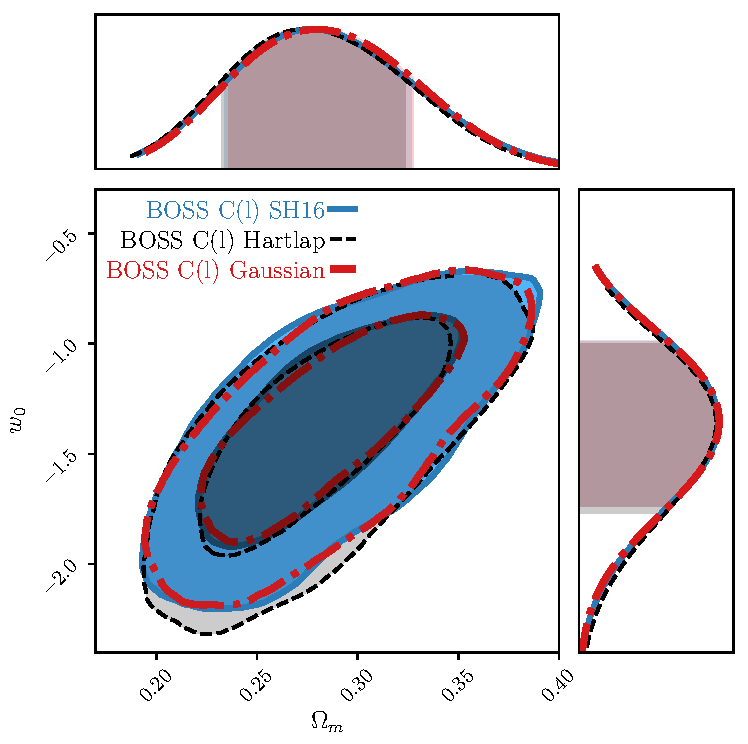
\includegraphics[scale=0.73]{BOSS-FIGS/likelihood_comparisonOmega_cdm_w0.pdf}
\caption[Comparison between the three likelihood methods mentioned in Section \ref{Sec:LikelihoodsPriors} using the BOSS $C_{\ell}$ data only for $\Omega_{m}$ and $w_0$.]{Comparison between the three likelihood methods mentioned in Section \ref{Sec:LikelihoodsPriors} using the BOSS $C_{\ell}$ data only for $\Omega_{m}$ and $w_0$ in a $w$CDM model: Gaussian (red), Gaussian with Hartlap correction (black) and the SH16 (blue) likelihoods. Note how, given the high number of log-normal simulation used to estimate the inverse of the covariance, the Hartlap correction likelihood, SH16, and Gaussian have equivalent contours even though the sampled parameters and likelihood values are different. It is clear from this analysis that the estimated covariance matrix from Section \ref{Sec:Cov} is robust and was estimated with a sufficient number of simulations.}
\label{fig:LikelihoodCompare}
\end{center}
\end{figure}

\qquad In order to perform a robust analysis, the three likelihoods approaches were implemented: Gaussian, Gaussian using the Hartlap correction, and the SH16 t-distribution likelihood. Although the values of the sampled parameters and posterior values were different, the Gaussian + Harlap correction, the SH16, and the Gaussian likelihoods led to very similar cosmological contours. Figure \ref{fig:LikelihoodCompare} shows a comparison between the three likelihood for a $w$CDM
model, using the BOSS $C_{\ell}$'s only, for $w_0$ and $\Omega_m$. In all of the following results in this Section, I use the SH16 likelihood.


%------------------------------------------------------------------------%
%                        	CONSISTENCY CHECKS 
%------------------------------------------------------------------------%
\section{Consistency Checks}
In this section, I perform a series of consistency checks in order to assess the validity of the cosmological parameter estimation pipelines and data samples. 

\subsection{Parameter-dependant Theoretical Covariance Matrix}
\begin{figure}
\begin{center}
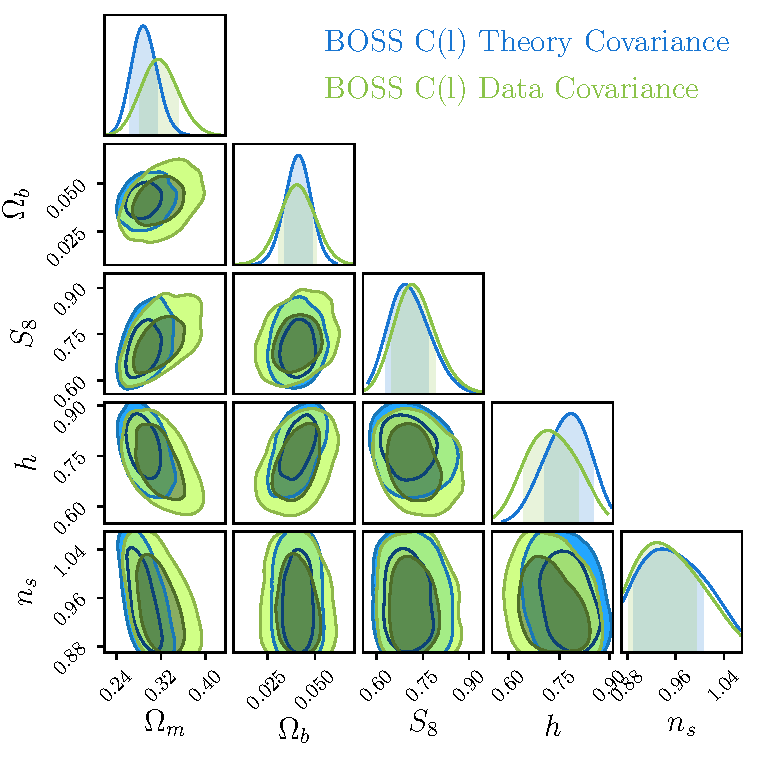
\includegraphics[scale=0.75]{BOSS-FIGS/theoryCovContours.pdf}
\caption[Comparison between $\Lambda$CDM cosmologies recovered using the covariance matrix estimated in Section \ref{Sec:Cov}and the cosmology dependent theoretical covariance matrix from Equation \eqref{Eq:TheoVariance}.]{Comparison between $\Lambda$CDM cosmologies recovered using the covariance matrix estimated in Section \ref{Sec:Cov} (\textit{green contours}, same as the ones from Section \ref{Sec:LCDM}), and the cosmology dependent theoretical covariance matrix from Equation \eqref{Eq:TheoVariance} (\textit{blue contours}). Note that the same parameters were sampled in both cases as the theoretical covariance also depends on the same nuisance parameters. These marginalised credible intervals (CI) 1- and 2-$\sigma$ plots indicate both the estimated covariance matrix and the \uclcl pipeline robustness.}
\label{fig:TheoryCovTriangle}
\end{center}
\end{figure}

An alternative likelihood was implemented in the \uclcl pipeline, based on the theoretical expression I derived for the covariance matrix (Section \ref{Sec:TheoCov}, Equation \eqref{Eq:TheoVariance}) where the signal angular power spectra, $S_{\ell}$, also depends on the sampled parameters. Most standard cosmological analysis in the literature \citep{2016BOSSCosmology,2017arXiv170801530D,2017MNRAS.465.1454H} assume a covariance matrix which is independent of cosmology and which is estimated for a fiducial simulation. Here, I do not expect to obtain the same cosmological contours from this method as those presented in the section that follow; however, I do not expect the contours from this method to disagree significantly with the ones obtained with my estimated covariance matrix. Figure \ref{fig:TheoryCovTriangle} shows the results for this test for a $\Lambda$CDM cosmological model. 

\subsection{Controlled Cosmology Pipeline Test}\label{Sec:ConsistControl}
\begin{figure}
\begin{center}
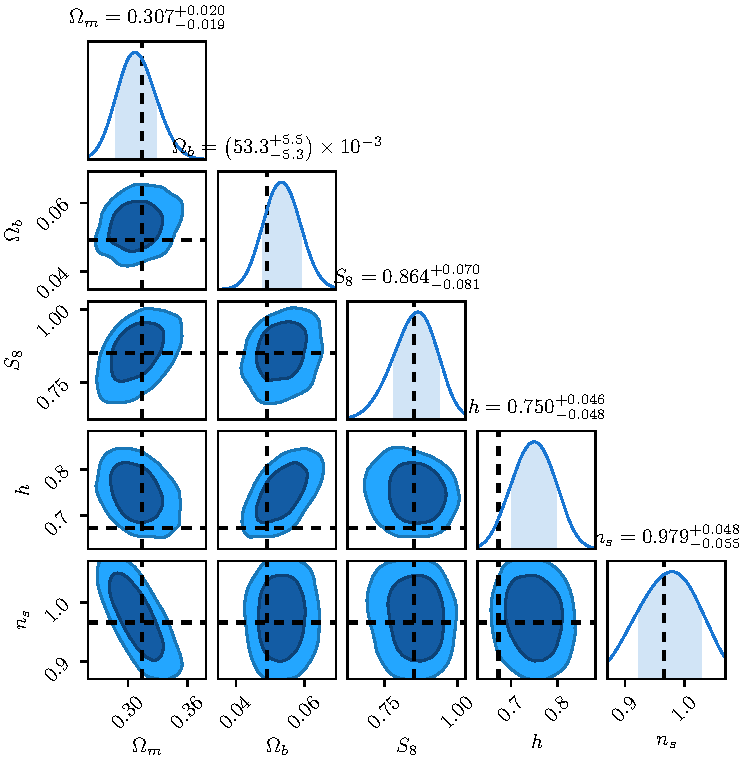
\includegraphics[scale=0.85]{BOSS-FIGS/Controlled_PipelineTest.pdf}
\caption[Cosmological constraints recovered from a controlled cosmology pipeline test.]{Cosmological constraints recovered from a controlled cosmology pipeline test. The dashed lines denote the Planck-like cosmology used as input in the simulations analysed in the blue contours. All parameters agree in within the estimated error-bars.}
\label{fig:Controlledtest}
\end{center}
\end{figure}

For this test, I generated theory autos- and cross- $C_{\ell}$s to mimic the BOSS dataset using a Planck-like cosmology: $h = 0.6725$, $\Omega_b = 0.0492$, $\Omega_{m} = 0.314$, $w_0 = -1.0$, $S_8 = 0.830$, $n_s = 0.96575$. I simulated these fiducial power spectra using the BOSS redshift distribution $n(z)$ from Figure \ref{fig:NZ_BOSS}. I chose the nuisance parameters to match the best fit values obtained in Section \ref{Sec:LCDM} from the combination of the entire cosmological dataset available. Using BOSS masks as input, I created \flask mocks like as described in Section \ref{Sec:Cov}: generating the mocks at higher resolution, degrading them, and creating galaxy overdensity maps. I applied the PCL estimator on the 13 overdensity maps, calculating the auto- and cross- power spectra as described for the data in Section \ref{Sec:Measurements}.

\qquad Finally, I ran a cosmological parameter estimation for a $\Lambda$CDM cosmology, varying also the 28 BOSS nuisance parameters and using the theoretical covariance matrix as in the previous section. The results are shown in Figure \ref{fig:Controlledtest}, where the recovered parameters are within the errors with no indications of biases in the entirety of the pipeline. 

\subsection{Internal Checks: Single Redshift Bin Consistency}
To test the data's internal consistency, I performed a full cosmological analysis in each individual redshift bin from the BOSS samples. The test was performed using a $\Lambda$CDM model, varying the same nuisance parameters as described in Section \ref{Sec:LikelihoodsPriors} for each bin: redshift dispersion, bias, and extra shot noise for the last two CMASS bins. If each individual bin is consistent with all others, this indicates that one can obtain cosmological constraints from the combination of the individual bins. This is shown in Figure \ref{fig:SiingleBinAnaly} for the posterior projections of $\Omega_m$ and $\Omega_b$. In these figures, all contours overlap and, even though some tomographic redshift bins prefer a secondary peak they are consistent across the redshift bins. This secondary peak is due to a known cosmological parameter degeneracy \citep{2001Percival}.

\begin{figure}
\begin{subfigure}{.5\textwidth}
  \centering
  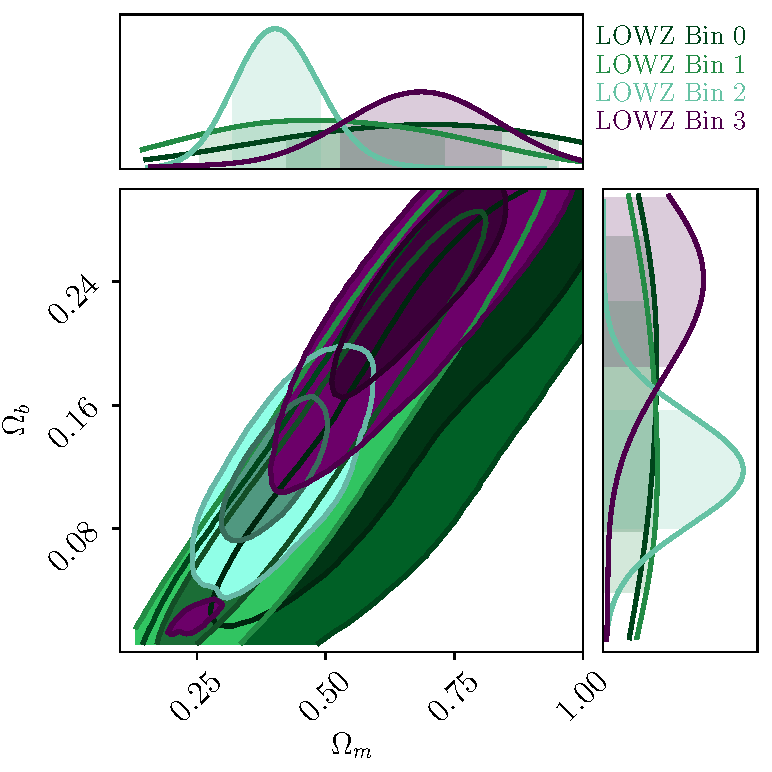
\includegraphics[width=\columnwidth]{BOSS-FIGS/LOWZ_SINGLE_BIN_1.pdf}
  \caption{}
\end{subfigure}%
\begin{subfigure}{.5\textwidth}
  \centering
  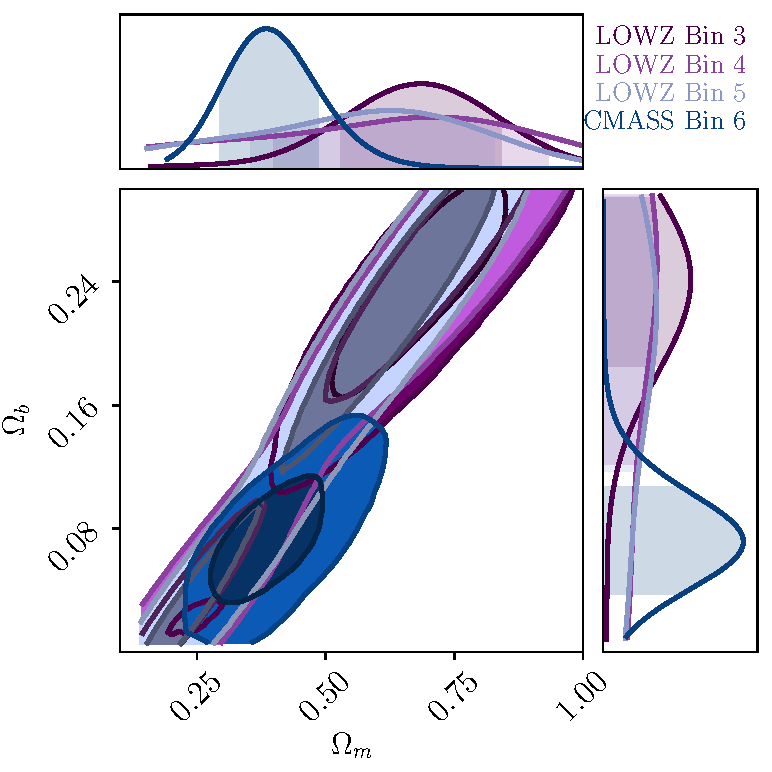
\includegraphics[width=\columnwidth]{BOSS-FIGS/LOWZ_SINGLE_BIN_2.pdf}
  \caption{}
\end{subfigure}\\
\begin{subfigure}{.5\textwidth}
  \centering
  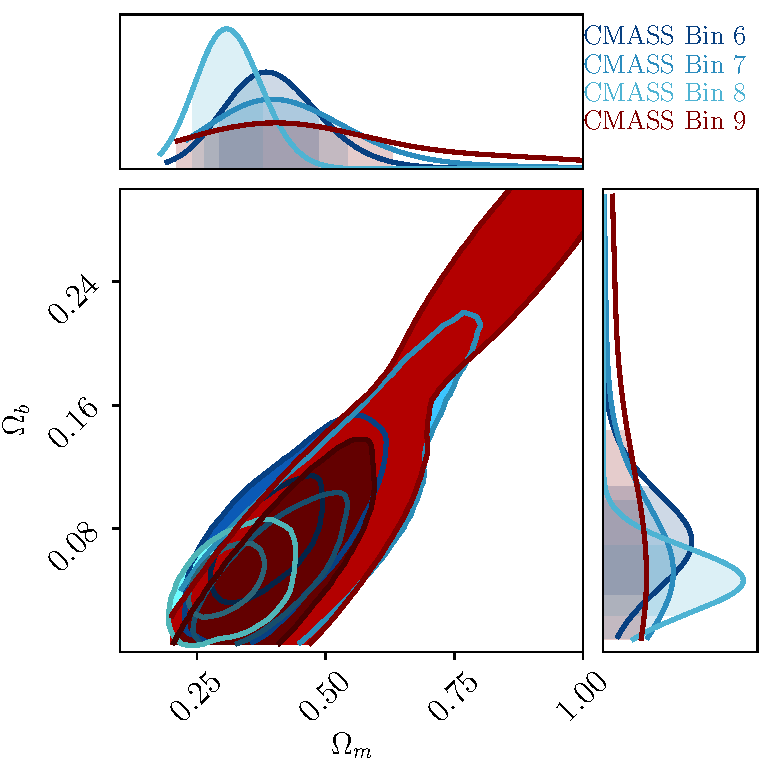
\includegraphics[width=\columnwidth]{BOSS-FIGS/CMASS_SINGLE_BIN_1.pdf}
  \caption{}
\end{subfigure}%
\begin{subfigure}{.5\textwidth}
  \centering
  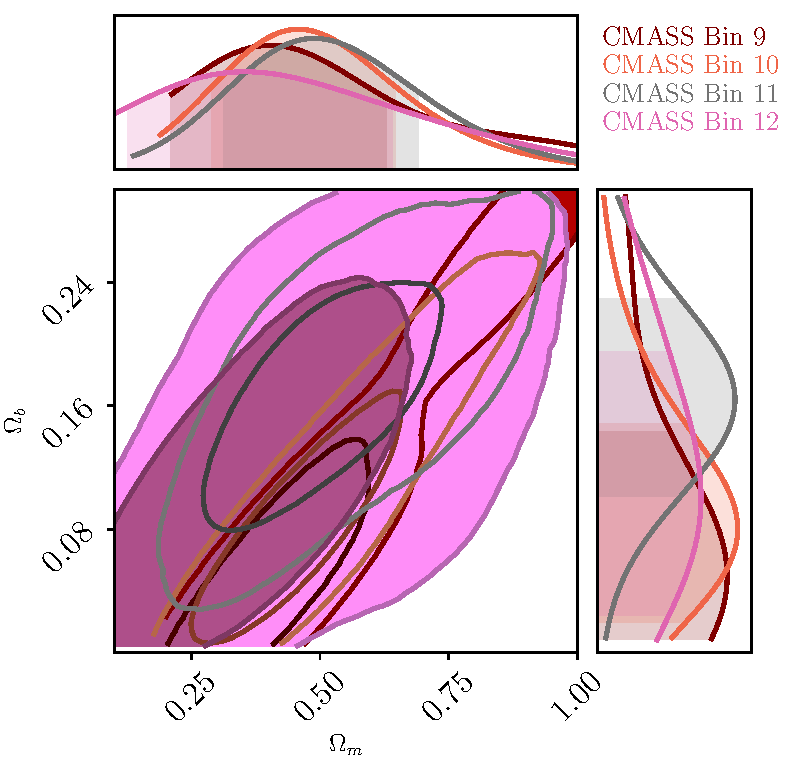
\includegraphics[width=\columnwidth]{BOSS-FIGS/CMASS_SINGLE_BIN_2.pdf}
  \caption{}
\end{subfigure}%
\caption[Consistency checks for single tomographic redshift bins for all LOWZ and CMASS bins using the $\Omega_b\,  \times \, \Omega_{m}$ contours]{Consistency checks for single tomographic redshift bins for all LOWZ and CMASS bins. Here, I show the $\Omega_b\,  \times \, \Omega_{m}$ contours taken from a $\Lambda$CDM cosmological inference, i. e. varying the same cosmological parameters as the ones from Section \ref{Sec:LCDM}. \textit{(a)} Shows LOWZ-0, LOWZ-1, LOWZ-2, and LOWZ-3 tomographic bins; \textit{(b)} shows LOWZ-3, LOWZ-4, LOWZ-5, and CMASS-6 tomographic bins; \textit{(c)} shows CMASS-6, CMASS-7, CMASS-8, and CMASS-9 tomographic bins; and \textit{(d)} shows CMASS-9, CMASS-10, CMASS-11, and CMASS-12 tomographic bins.}
\label{fig:SiingleBinAnaly}
\end{figure}

\subsection{Distribution of Residuals}
For a dataset with uncorrelated errors (diagonal covariance matrix), the vector of normalised residuals is given by:

\begin{equation}
R = \Xi^{-1}(D - T(\vec{\theta}))
\label{Eq:Residuals_1}
\end{equation}
where $\Xi$ is a diagonal matrix containing the square roots of the variances, $D$ is the data vector and $T(\vec{\theta})$ is the theory vector for a given parameter vector $\vec{\theta}$. If $T(\vec{\theta})$ represents the true model, and the true errors are known, the residuals are by definition given by a Gaussian with $\mu=0$ and $\sigma=1$ \citep{chisq2010}. On the other hand, if the errors are estimated from the data, the residuals are given by a Student's t-distribution. This distribution approaches a Gaussian with increasing number of data points. If this distribution shows a significant deviation from a Gaussian, the model is ruled out. If it follows a Gaussian distribution, one either found the true model, or the current data is not enough to distinguish between the model found and the true model \citep{chisq2010}.

\qquad When the covariance matrix is not diagonal (the errors are correlated), Equation \eqref{Eq:Residuals_1} is no longer true and one has to deal with the full covariance matrix. In order to get back to a diagonal matrix, the covariance matrix can be written in terms of its eigen-decomposition :

\begin{equation}
C = Q \Lambda Q^{-1}
\end{equation}
where $Q$ is the matrix of eigenvectors and $\Lambda$ is the diagonal matrix containing the eigenvalues of $C$. The inverse is then given by $C^{-1} = Q \Lambda^{-1} Q^{-1}$, which transforms the $\chi^2$ into:

\begin{equation}
\chi^2 = \big[ \hat{S}_{\Delta\ell} - S^{th}_{\Delta\ell}(\pmb{\Theta}, \pmb{\nu})\big]^T Q \Lambda^{-1} Q^{-1} \big[ \hat{S}_{\Delta\ell} - S^{th}_{\Delta\ell}(\pmb{\Theta}, \pmb{\nu})\big]
\end{equation}
If $\Lambda$ is treated as the new (diagonal) covariance matrix, it follows that the normalised residuals are now given by:

\begin{equation}
R = \Xi^{-1} Q^{-1} \big[ \hat{S}_{\Delta\ell} - S^{th}_{\Delta\ell}(\pmb{\Theta}, \pmb{\nu})\big]
\label{Eq:Residuals_2}
\end{equation}
where $\Xi$ now contains the square roots of the eigenvalues.%($\sqrt[]{\lambda_n}$). 

\qquad In this test, Equation \eqref{Eq:Residuals_2} is used to calculate the residuals at the best-fit point in a flat $\Lambda CDM$ Cosmology and plot the results in a histogram (Figure \ref{fig:Residuals}). There are no significant deviations from a Gaussian with $\mu=0$ and $\sigma=1$, which means the model seems to be a very good representation of the data.

\begin{figure}
\begin{center}
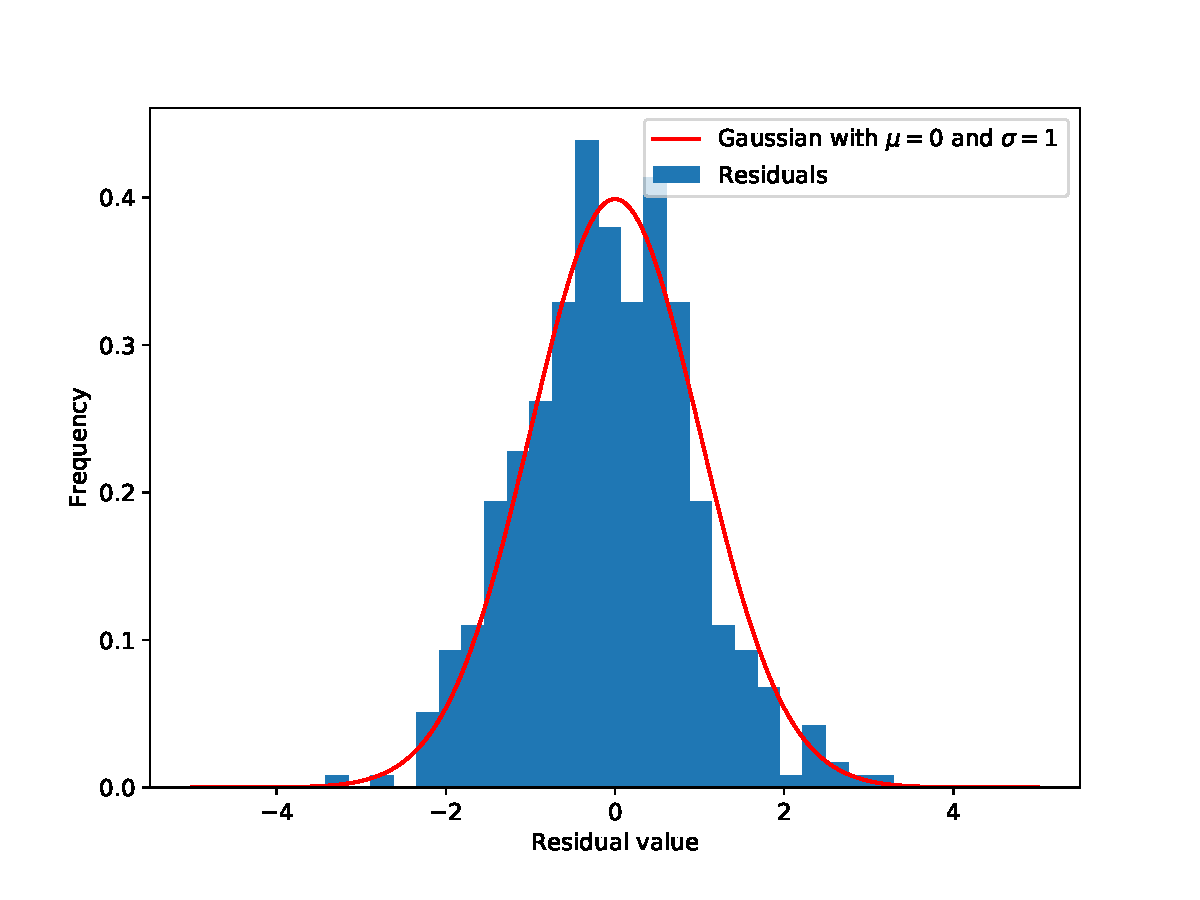
\includegraphics[scale=0.60]{BOSS-FIGS/chi_lcdm_new.pdf}
\caption[Distribution of residuals for the best-fit point in a flat $\Lambda$CDM models.]{Comparison between the histogram of the distribution of residuals (given by Equation \eqref{Eq:Residuals_2}) calculated at the best-fit point in a flat $\Lambda$CDM cosmology (see Section \ref{Sec:LCDM}) and a Gaussian with $\mu=0$ and $\sigma=1$. As this distribution does not show any significant deviation from the Gaussian, the model is either the truth or the current data cannot make any further distinction between the model and the truth.} 
\label{fig:Residuals}
\end{center}
\end{figure}

\section{External data}\label{Sec:ExternalData}

I compared and combined the results in this chapter with results obtained from the Planck satellite CMB experiment \citep{PlanckResults2015}, and Type Ia Supernovae from the Joint Light curve Analysis (JLA) collaboration \citep{JLAdata}. The relevant likelihood codes for these probes were implemented and tested in the \uclcl pipeline. The results from these external datasets were checked against the official cosmological results from the relevant collaborations. I have recovered the published cosmological parameters with the \uclcl pipeline which allowed me to use and combine them with the BOSS angular power spectra.

\qquad The CMB data from Planck was added through the Planck likelihood codes \texttt{Commander} and \texttt{Plik} \citep{PlanckLikelihood2015}. For low multipoles, in the range $l=2-29$, \texttt{Commander} is used with temperature (TT) and polarization auto- and cross- power spectra (BB, TB, EB). For high multipoles, in the range $l=30-2508$, \texttt{Plik} is used with temperature (TT) and polarization auto- and cross- power spectra (TE, EE). This configuration is commonly referred to as Planck TT,TE,EE+lowP. \texttt{Plik} also introduces 94 additional nuisance parameters. In order to reduce this large parameter space, the lite version of the data offered by the Planck Collaboration was used. This lite version allows to compute a nuisance marginalized CMB likelihood. The only CMB nuisance parameter left is the Planck absolute calibration parameter ($y_{cal}$). I sample this parameter in all the runs that include Planck data. The Planck likelihood codes were added to \texttt{UCLPI} and all the Planck results presented have been obtained using this pipeline. I show in the all cosmological contours and in table \ref{tab:LCDM_Constraints} that this pipeline reproduces the cosmological results found by the Planck Collaboration \citep{PlanckCosmology2016}.

\qquad The SN data from JLA was added to the \texttt{UCLPI} pipeline through the likelihood code provided by the JLA Collaboration \citep{JLAdata}. This likelihood code needs the luminosity distances to the 740 Supernovae in the sample and 4 nuisance parameters ($\alpha, \beta, M_B, \Delta_M$) described in \cite{JLAdata}. The luminosity distances are calculated by \class \citep{Class} using the redshifts of the supernovae within a given Cosmology (set by the sampled cosmological parameters). I sample the absolute magnitude at peak brightness ($M_B$) as part of the analysis, and keep the other 3 nuisance parameters fixed to their best-fit values found by \cite{JLAdata} since these have a small impact in the cosmological parameters when combined with the BOSS dataset.

\qquad I also implemented a BAO likelihood in order to compare my results with the official \textbf{BOSS Consensus} results from \cite{2016BOSSCosmology}. This measurements use 3 redshift bins with $z_{eff} = 0.38, \, 0.51, \, \text{and} \, 0.61 $, where I used the full shape post-reconstruction measurements from the correlation function and 3D power spectra, which contains additional information from measurements of $f\sigma_8$ (see table 7 from \cite{2016BOSSCosmology}). I have not combined these results with my BOSS results, but I plot them alongside my results alone in the next sessions to give the reader an impression of how my results compare with the BOSS alone results from \cite{2016BOSSCosmology}.

%-----------------------------------------------------------------------%
%                        	COSMOLOGY: LCDM
%-----------------------------------------------------------------------%
\section{Cosmological Analysis}\label{Sec:CosmoAnal}
\subsection{Flat $\Lambda$CDM Constraints}\label{Sec:LCDM}
Here, I obtain constraints for the standard cosmological model, a flat $\Lambda$CDM cosmology. I fixed the curvature of the universe to zero, e.g. $\Omega_k = 0$, and varied five cosmological parameters: the baryonic density, $\Omega_b$; the dark matter density, $\Omega_{cdm}$; the amplitude of the primordial power spectra, $A_s$; the spectral index, $n_s$; and the Hubble constant, $h$. As this model considers dark energy as the cosmological constant $\Lambda$, I fixed the $w_0$ parameter to a cosmological constant ($w_0 = -1$), therefore: $\Omega_{\Lambda} = 1 - (\Omega_b + \Omega_{cdm})$. Here, I also fixed the sum of neutrino masses to the minimum found from neutrino oscillation experiments, $\sum m_{\nu} = 0.06 \, eV$ -- the lower bound as suggested from neutrino oscillation experiments \citep{2006NeutrinoReview,2014NeutrinoCosmoPlanck}. Following, I also obtained derived parameters as the total matter density, $\Omega_m \equiv \Omega_b + \Omega_{cdm}$; and the fluctuation of amplitude at 8 $h^{-1}$Mpc, $\sigma_8$ or $S_8 = \sigma_8\sqrt{\Omega_m/0.3}$. Finally, as described in the previous section, I varied the BOSS, Planck and JLA nuisance parameters. For this analysis, I used the $\ell_{max}^{5\%}$ cuts (see table \ref{Tb:EllCuts}).

\qquad I checked the consistency of the datasets by running the same analysis for these probes alone and combined (Planck, JLA, and Planck plus JLA) and calculating the respective Bayes factors for these cosmological constraints. The Bayes factor, Equation \eqref{Eq:BayesFactor},  for combinations of the considered datasets indicates consistency between all three probes:

\begin{align}
R_{\scriptscriptstyle\text{BOSS+JLA}}^{\Lambda CDM} & \simeq 18  \\
R_{\scriptscriptstyle\text{BOSS+PLANCK}}^{\Lambda CDM} & \simeq 74 \\
R_{\scriptscriptstyle\text{PLANCK+JLA}}^{\Lambda CDM} & \simeq 11 \\
R_{\scriptscriptstyle\text{BOSS+PLANCK+JLA}}^{\Lambda CDM} & \simeq 4 \times 10^4
\end{align}
these indicate that the datasets are compatible for the considered model, given the chosen priors.

\begin{figure}
\begin{center}
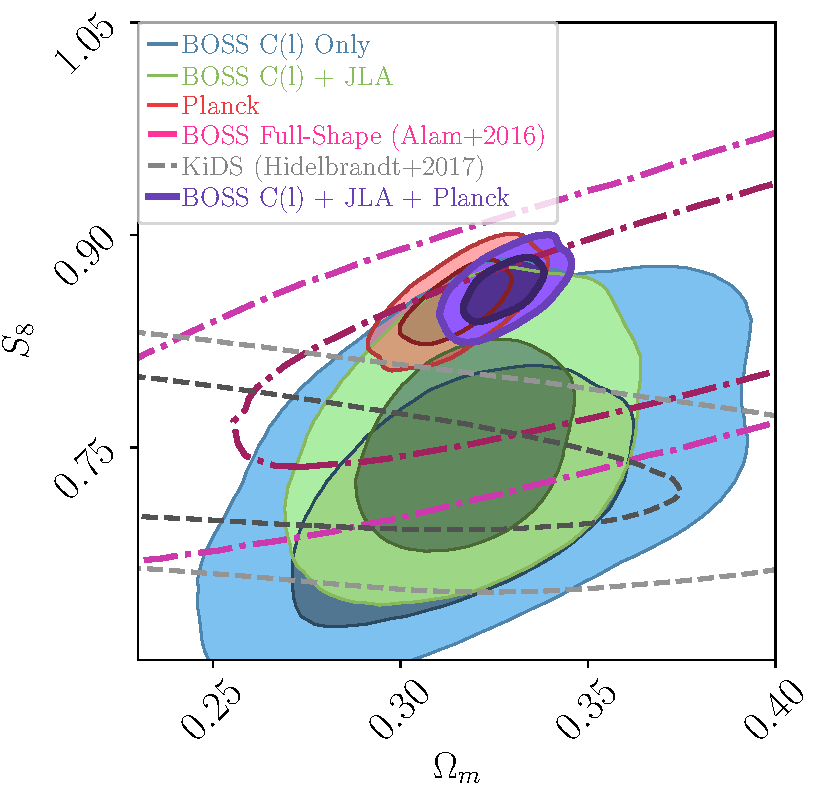
\includegraphics[scale=0.70]{BOSS-FIGS/LCDM_External_KidsOmega_m.pdf}
\caption[2D $\Omega_m \, \times \, S_8$ marginalised credible intervals for a $\Lambda$CDM cosmology.]{2D $\Omega_m \, \times \, S_8$ marginalised credible intervals for a \textbf{$\Lambda$CDM cosmology}. In this figure I show in detail the cosmological results from Section \ref{Sec:LCDM} for BOSS $C_{\ell}$s only \textit{(blue)}; BOSS $C_{\ell}$s plus JLA \textit{(green)}; BOSS $C_{\ell}$s plus JLA and Planck \textit{(purple)}; together with results using the post-reconstruction full shape (incl. $f\sigma_8(z)$) from \protect\cite{2016BOSSCosmology} consensus results \textit{(pink)}, and Planck alone \textit{(red)}. In order to compare these results to a weak-lensing probe, I also show here the results from \protect\cite{2017MNRAS.465.1454H} \textit{(grey, dashed)}. For details about the external datasets, see Section \ref{Sec:ExternalData}.}
\label{fig:Om_S8_LCDM}
\end{center}
\end{figure}

\qquad Finally, when considering the combination of BOSS $C_{\ell}$s, Planck and JLA, I find results consistent with \cite{2016BOSSCosmology,2017MNRAS.465.1454H,2017arXiv170801530D}. Figure \ref{fig:Om_S8_LCDM} shows the $\Omega_m \, \times \, S_8 $ 2D plane for this analysis and comparisons with Planck and the BOSS full-shape post-reconstruction from \cite{2016BOSSCosmology}. Despite the Bayes factors showing no significant reason to be concerned about the compatibility of these datasets, an interesting trend in this figure can be seen insofar as a tension and the BOSS dataset in this work preferring a smaller $S_8$ than the Planck analysis. I argue here that this method would prove potentially very useful in resolving any $S_8$ tensions which exist currently between CMB and weak lensing data \citep{2015MacCrann,2017CharnockTension}.

\qquad The results for the 1D marginalised cosmological constrains for BOSS $C_{\ell}$ and combinations, together with the 68\% credible intervals can be found in table \ref{tab:LCDM_Constraints}. The 1-$\sigma$ and 2-$\sigma$ contour levels can be found in Figure \ref{fig:LCDM_Cosmology} where the nuisance parameters have been marginalised over. Figure \ref{fig:Cl_Bestfit} shows the best fit theory $C_{\ell}$ using the parameters estimated from this analysis with a $\chi^2_{red} = 1.08$, which also indicates reliability and robustness of the analysis performed. 

\qquad Even though I do not show the results in this work, I performed a cosmological analysis using a $\Lambda$CDM with a fixed zero neutrino mass, $\sum m_{\nu} = 0$ eV. I compared it with the model used in this section, $\Lambda$CDM with $\sum m_{\nu}$ fixed to $0.06$ eV, using the Bayes factor for model selection. Consider $\vec{D}$ representing the combination of data vectors; the Bayes factor is given by

\EQ{}{
R_{A,B} = \frac{\mathcal{Z}(\vec{D}_{\scriptscriptstyle\text{BOSS+PLANCK+JLA}}|\sum m_{\nu} = 0.06 \text{ eV})}{\mathcal{Z}(\vec{D}_{\scriptscriptstyle\text{BOSS+PLANCK+JLA}}|\sum m_{\nu} = 0 \text{ eV}) } = 8\times 10^5
}
\noindent This indicates that, for a $\Lambda$CDM model, the data prefers massive neutrinos over no neutrino mass at all.


\begin{figure*}
\begin{center}
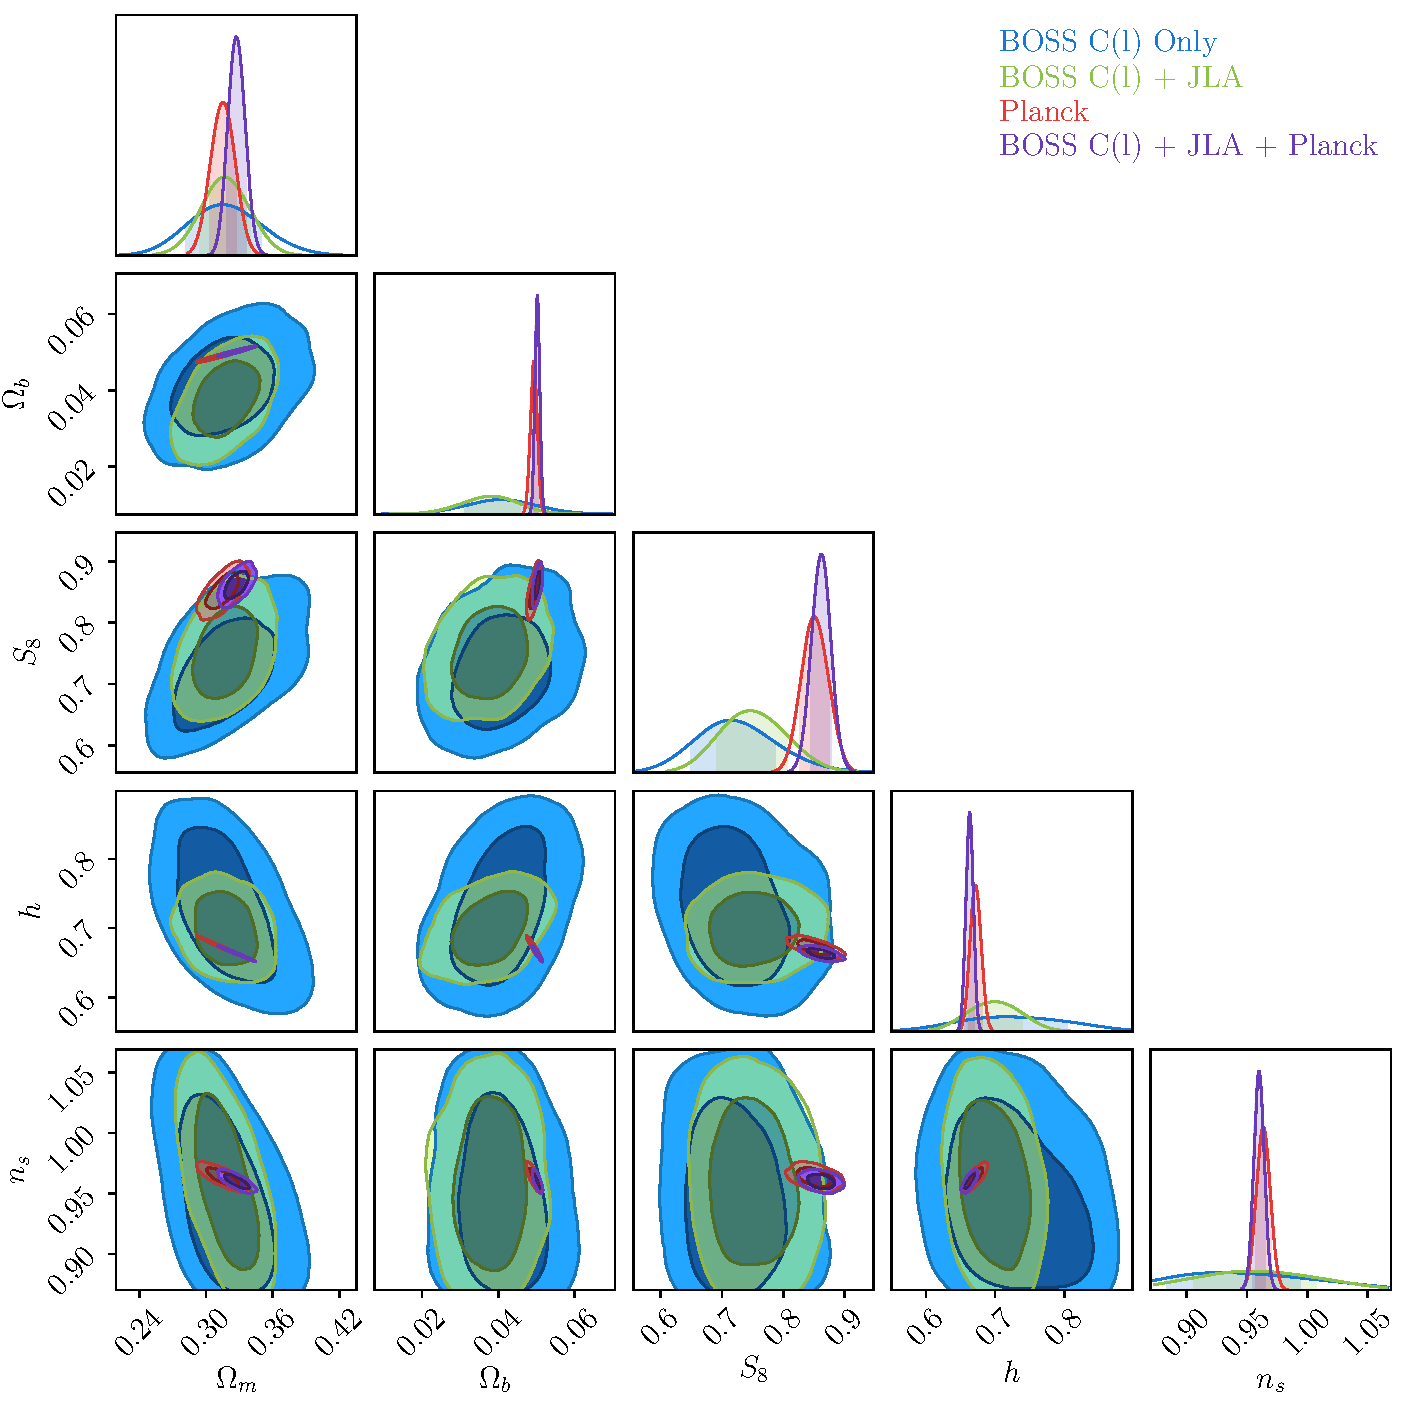
\includegraphics[width=\textwidth]{BOSS-FIGS/LCDM_Cosmology.pdf}
\caption[Marginalised 1 \& 2D cosmological constraints for the $\Lambda$CDM model.]{Marginalised 1 \& 2D cosmological constraints for the \textbf{$\Lambda$CDM model} varying five cosmological parameters with 1-$\sigma$ (darker) and 2-$\sigma$ (lighter) contour levels. I show here a combination of sampled and relevant derived parameters: $\Omega_m$, $\Omega_b$, $S_8$, $h$, and $n_s$ (marginalising over $\tau_{reio}$ for the Planck combinations). The \textit{blue contours} where estimated from the BOSS $C_{\ell}$s data alone using the SH16 likelihood; \textit{the green contours} are a combination the BOSS likelihood and JLA data (see Section \ref{Sec:ExternalData}); \textit{the red contours} are the Planck high-$\ell$ TT, TE, EE and low-$\ell$ P likelihood results (see Section \ref{Sec:ExternalData}); finally, the purple contours are a combination of the three probes: BOSS $C_{\ell}$, JLA and Planck (also high-$\ell$ TT, TE, EE and low-$\ell$ P). Note that none of the results here use Planck Lensing data.}
\label{fig:LCDM_Cosmology}
\end{center}
\end{figure*}

\begin{figure*}
\begin{center}
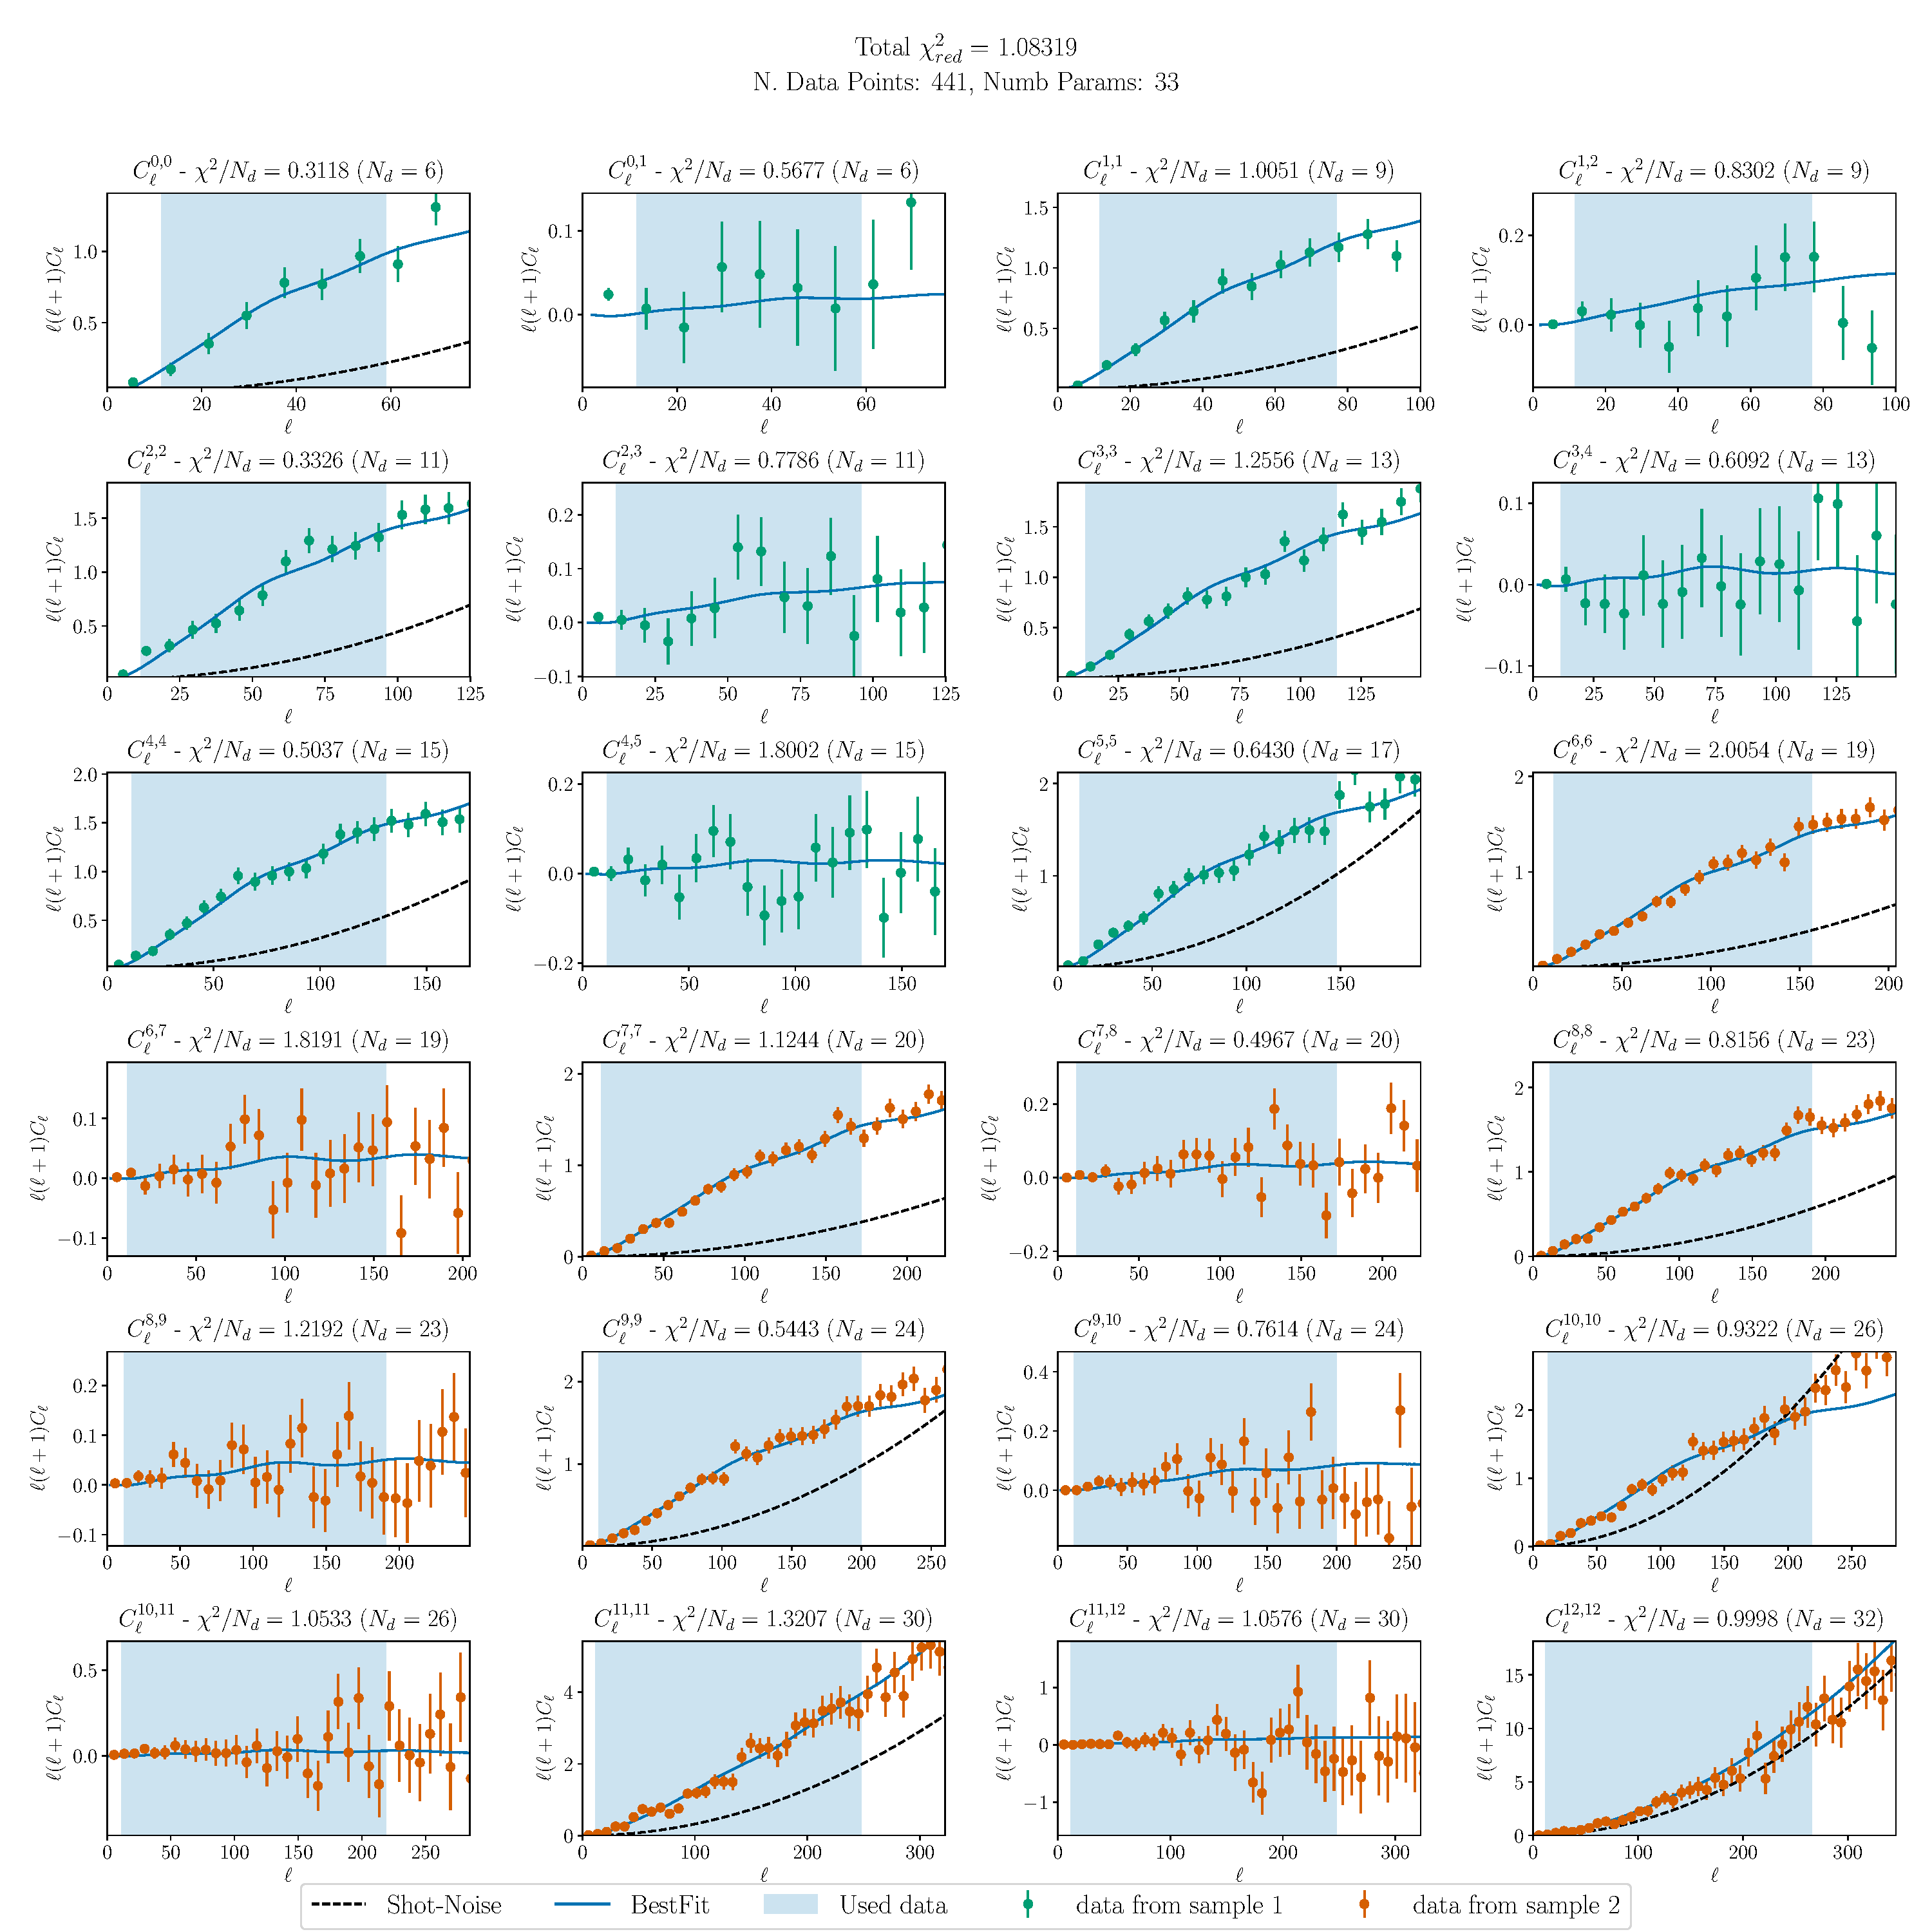
\includegraphics[width=1.05\columnwidth]{BOSS-FIGS/BestFit_LCDM.pdf}
\caption[BOSS measured $C_{\ell}$s and the best-fit theory from the $\Lambda$CDM model.]{Auto- and cross- angular power spectra for the 13 tomographic redshift bins considered for the BOSS DR12 samples: LOWZ (sample 1) and CMASS (sample 2). The shaded blue regions show the scales considered in the cosmological parameter estimation in Section \ref{Sec:CosmoBananas}. The \textit{data points} are the pseudo-$C_{\ell}$ estimates, described in Section \ref{Sec:Measurements}, for LOWZ and CMASS. The \textit{solid blue lines}, generated with \texttt{UCLCL}, reflect the \textit{best fit} auto- and cross-power spectra for the \textbf{$\Lambda$CDM model} estimated in Section \ref{Sec:LCDM}. Finally, the \textit{black dashed lines} show both shot noise and sampled shot noise (for bins 11 and 12). The overall reduced $\chi^2$ for this fit is $\chi^2_{red} \approx 1.08$, where the number of data points is 441 and the total number of sampled parameters is 33 -- 5 Cosmological parameters, and 28 nuisance parameters. The title on each individual plot reflects the bins \textit{i \& j} for each $C^{ij}_{\ell}$, the $\chi^2$ per data point ($\chi^2/N_d$), and the number of data points for that individual angular power spectrum, $N_d$. The $\ell$-ranges used in this figure correspond to the $\ell_{max}^{5\%}$ in table \ref{Tb:EllCuts}. Most of the constraining power comes from the auto-power spectra. The cross-power spectra serve to constrain parameters related to the RSD by helping to break the degeneracy between the bias and $A_s$ while also probing the redshift dispersion due to the peculiar motion of galaxies (FoG).}
\label{fig:Cl_Bestfit}
\end{center}
\end{figure*}


%------------------------------------------------------------------------%
%                        	COSMOLOGY: wCDM
%------------------------------------------------------------------------%

\subsection{Flat $w$CDM Constraints}\label{Sec:wCDM}
In this section, I allowed the equation-of-state of dark energy, $w_0$, to vary. This is a trivial extension of the standard model of cosmology with just one extra parameter. If $w_0 = -1$, the solution indicates that the nature of dark energy is actually the cosmological constant, $\Lambda$. The procedure for this analysis followed in similar fashion as the one outlined in Section \ref{Sec:LCDM}, varying six parameters instead of five: $\Omega_b$, $\Omega_{cdm}$, $n_s$, $\ln 10^{10} A_s$, $h$, and the extra $w_0$. Note that, for this case, I am not varying $w_a$, i. e., I do not consider a redshift evolution in the equation-of-state of dark energy. Again, I fixed the neutrino parameter to $\sum m_{\nu} = 0.06 \, eV$ \citep{2006NeutrinoReview,2014NeutrinoCosmoPlanck}. Here, I used the same $\ell_{max}^{5\%}$ cuts as in the last section (see table \ref{Tb:EllCuts}).

\begin{figure}
\begin{center}
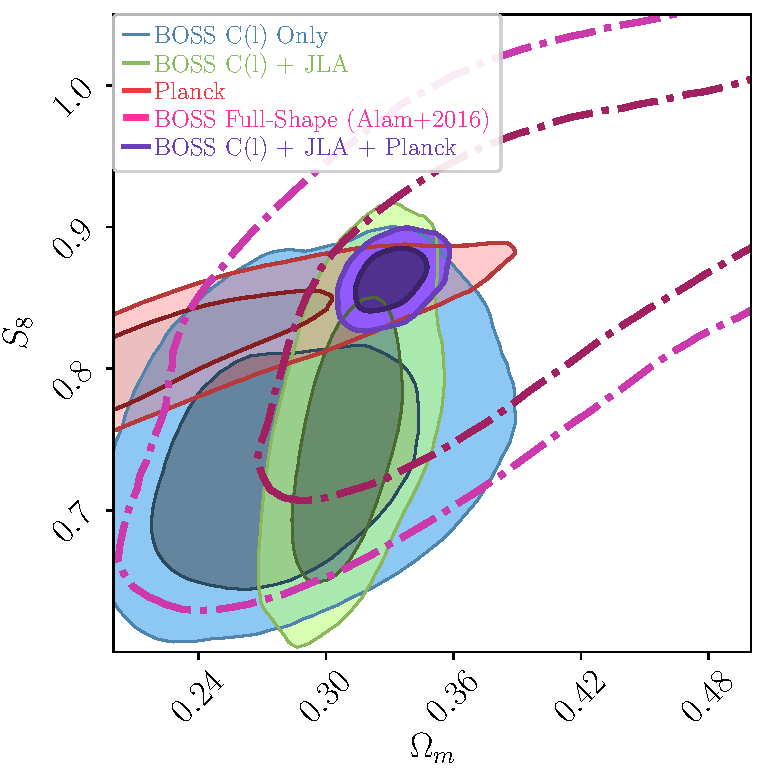
\includegraphics[scale=0.70]{BOSS-FIGS/Om_S8_wCDM.pdf}
\caption[2D $\Omega_m \, \times \, S_8$ marginalised credible intervals for a $w$CDM Cosmology.]{2D $\Omega_m \, \times \, S_8$ marginalised credible intervals for a \textbf{$w$CDM Cosmology}. This shows in detail the cosmological results from Section \ref{Sec:wCDM} for BOSS $C_{\ell}$s only \textit{(blue)}; BOSS $C_{\ell}$s plus JLA \textit{(green)}; BOSS $C_{\ell}$s plus JLA and Planck \textit{(purple)}; together with results using just the full shape (pre-reconstruction) from \protect\cite{2016BOSSCosmology} consensus results \textit{(pink)}, and Planck alone \textit{(red)}.}
\label{fig:Om_S8_wCDM}
\end{center}
\end{figure}

\qquad Figures \ref{fig:Om_S8_wCDM} and \ref{fig:Om_w0_wCDM} show in detail the contours for $S_8 \, \times \, \Omega_m$ and $w_0 \, \times \, \Omega_m$, respectively, and comparisons with previous measurements in the literature. From the Figure \ref{fig:Om_w0_wCDM} and from the complete set of results in \ref{fig:wCDM_Cosmology} I show that a $\sim 4\%$ error (1-$\sigma$ CI) on the equation-of-state of dark energy is obtained from this cosmological analysis:

\EQ{w0PlankBOSSJLA}{w_0 = -0.993^{+0.046}_{-0.043}.}
This results is consistent with the $\Lambda$CDM scenario of standard cosmology, i. e., it is consistent with dark energy being a cosmological constant, $\Lambda$. Note from Figure \ref{fig:wCDM_Cosmology} that I find a small value of $h$ (compared to \citealt{PlanckCosmology2016}) when combining BOSS $C_{\ell}$s, Planck, and JLA:

\EQ{}{h^{w\text{CDM}} = 0.661\pm 0.012.} This value is lower than the quoted Planck value alone; putting further tension in of this result if compared to the Hubble constant result from Cepheid Variables \citep{Riess2016, Riess2018}. 

\begin{figure}
\begin{center}
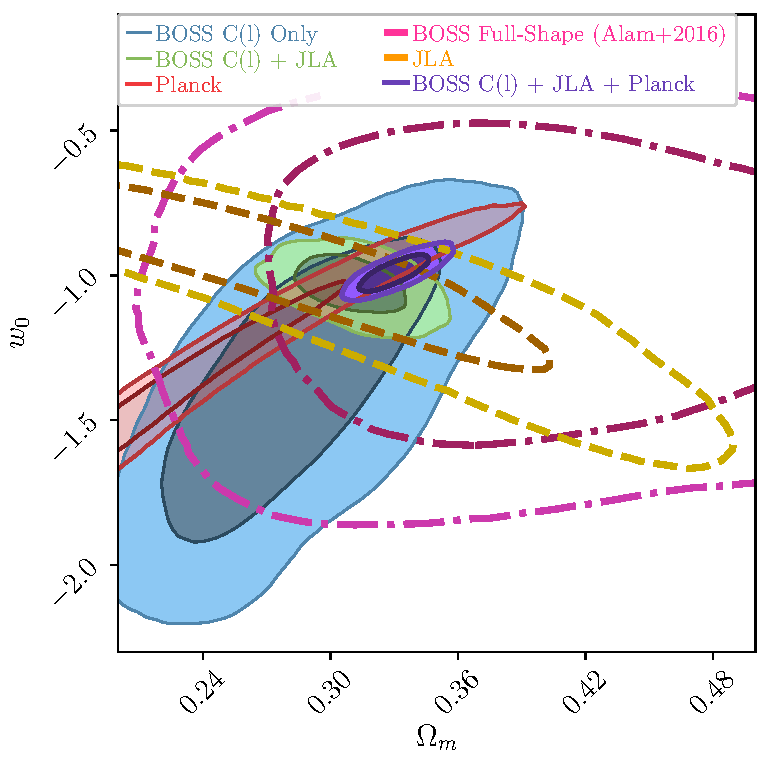
\includegraphics[scale=0.70]{BOSS-FIGS/w0_Om_wCDM.pdf}
\caption[2D $w_0 \, \times \, \Omega_m$ marginalised credible intervals for a $w$CDM Cosmology.]{2D $w_0 \, \times \, \Omega_m$ marginalised credible intervals for a \textbf{$w$CDM Cosmology}. This shows in detail the cosmological results from Section \ref{Sec:wCDM} for BOSS $C_{\ell}$s only \textit{(blue)}; BOSS $C_{\ell}$s plus JLA \textit{(green)}; BOSS $C_{\ell}$s plus JLA and Planck \textit{(purple)}; together with results using just the full shape (pre-reconstruction) from \protect\cite{2016BOSSCosmology} consensus results \textit{(pink)}, JLA \textit{(yellow)}, and Planck alone \textit{(red)}.}
\label{fig:Om_w0_wCDM}
\end{center}
\end{figure}

\qquad As the model in this section is different from the previous section, I performed an evidence analysis using the Bayes factor, Equation \eqref{Eq:BayesFactor}, in order to be sure that the measurements can be combined with the the external data described in Section \ref{Sec:ExternalData}. The following Bayes factors indicate that such combinations are consistent:

\begin{align}
R_{\scriptscriptstyle\text{BOSS+JLA}}^{\textit{w}CDM} & \simeq 2 \times 10^2  \\
R_{\scriptscriptstyle\text{BOSS+PLANCK}}^{\textit{w}CDM} & \simeq 4 \times 10^3 \\
R_{\scriptscriptstyle\text{PLANCK+JLA}}^{\textit{w}CDM} & \simeq 2 \\
R_{\scriptscriptstyle\text{BOSS+PLANCK+JLA}}^{\textit{w}CDM} & \simeq 3 \times 10^5
\end{align}

Finally, I used the ratio of the evidences, the Bayes factor, to perform a model selection between $w$CDM and $\Lambda$CDM using the final dataset combination. Assuming $\vec{D}$ to be the combination of data vectors for all the datasets, the Bayes factor between the two models is
\EQ{}{
R_{w,\Lambda} = \frac{\mathcal{Z}(\vec{D}_{\text{BOSS+Planck+JLA}}|w\text{CDM})}{\mathcal{Z}(\vec{D}_{\text{BOSS+Planck+JLA}}|\Lambda\text{CDM})} = 0.67
}
which does not significantly mean that one of the models is preferred over the other.

\begin{figure*}
\begin{center}
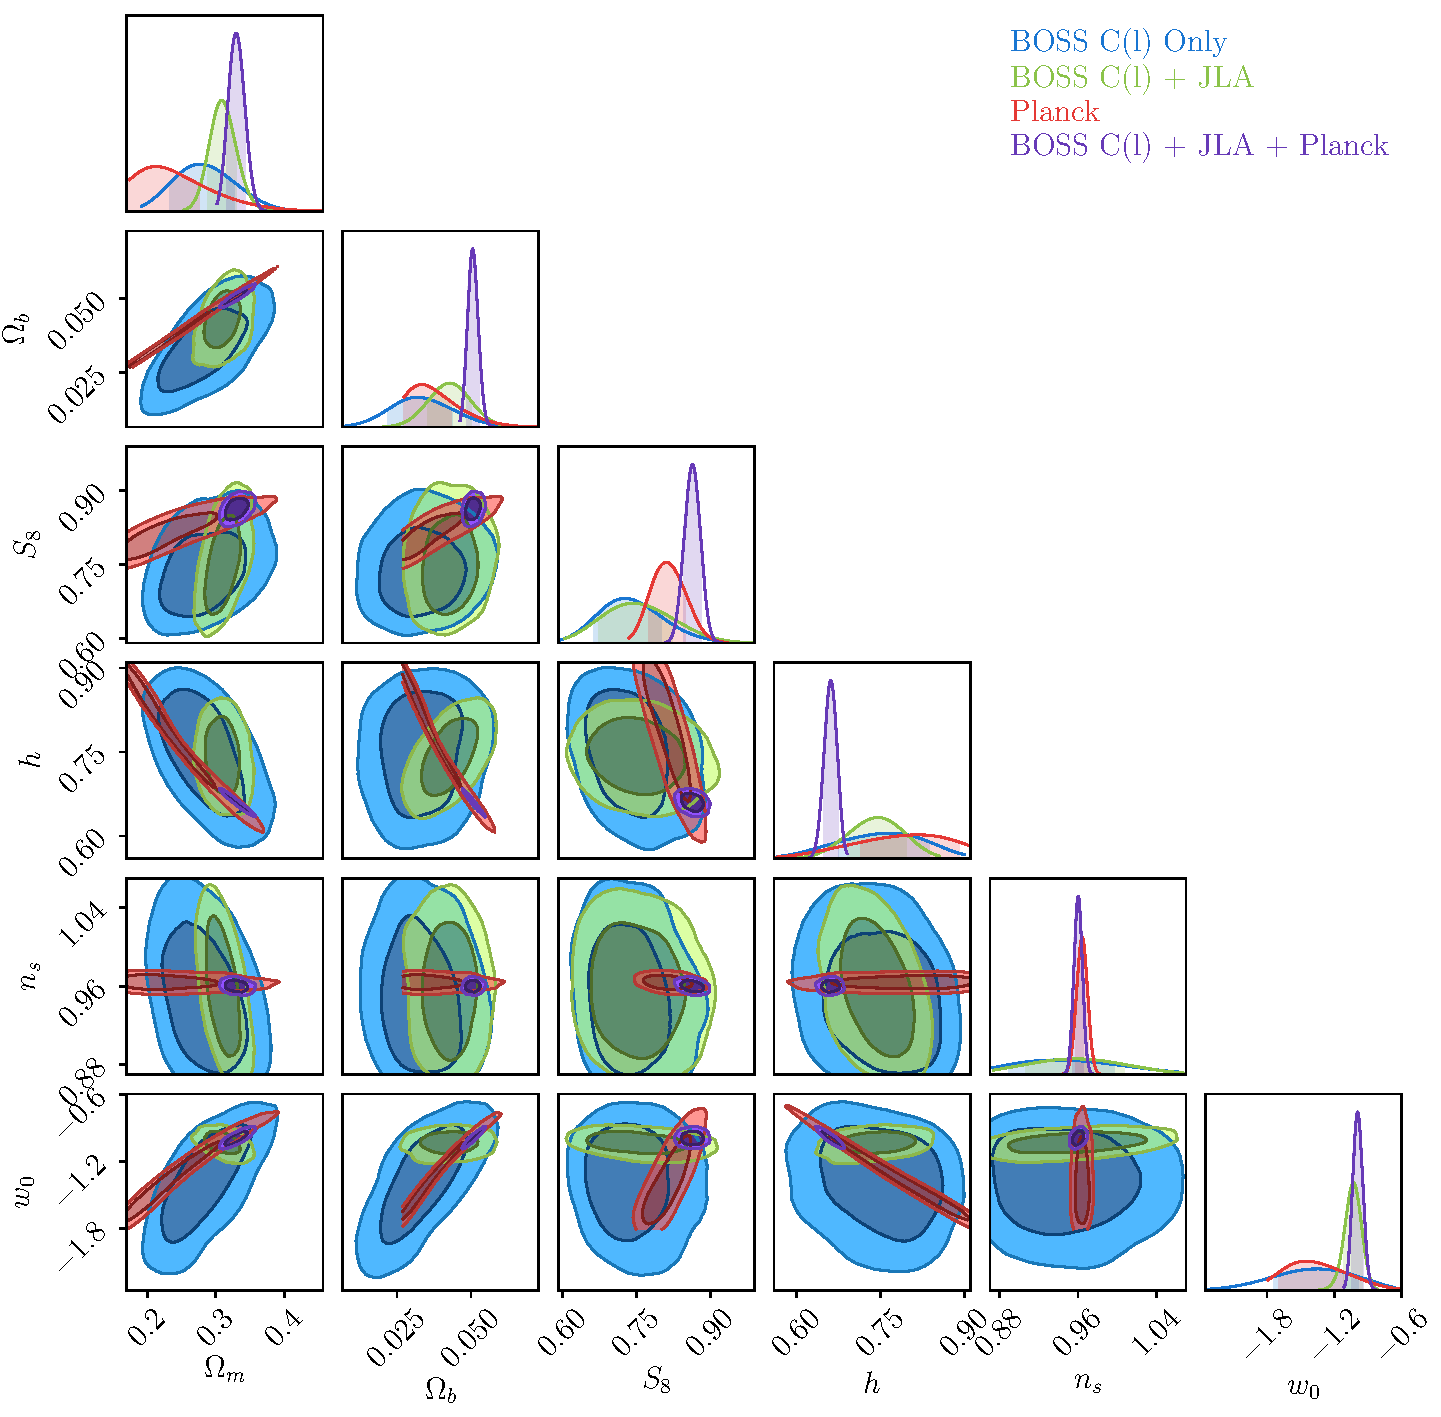
\includegraphics[width=\textwidth]{BOSS-FIGS/wCDM_Cosmology.pdf}
\caption[Cosmological constraints for the $w$CDM model.]{Cosmological constraints for the \textbf{$w$CDM model} varying now six cosmological parameters. This figure contains a combination of sampled and relevant derived parameters from the chains: $\Omega_m$, $\Omega_b$, $S_8$, $h$, $n_s$, and $w_0$. Note that the Planck chains also varied $\tau_{reio}$. The \textit{blue contours} where estimated from the BOSS $C_{\ell}$s data alone using the SH16 likelihood; \textit{green contours} are a combination the BOSS likelihood and JLA data; \textit{ red contours} are the Planck high-$\ell$ TT, TE, EE and low-$\ell$ P likelihood results; finally, the \textit{purple contours} are a combination of the three probes: BOSS $C_{\ell}$, JLA and Planck (also high-$\ell$ TT, TE, EE and low-$\ell$ P). The apparent cuts in the Planck alone contours are due to the prior in $h$. Note, again, that none of the results here use Planck Lensing data.}
\label{fig:wCDM_Cosmology}
\end{center}
\end{figure*}

%------------------------------------------------------------------------%
%                        	COSMOLOGY: LCDM + NEUTRINOS
%------------------------------------------------------------------------%

\subsection{Flat $\Lambda$CDM + $\sum m_\nu$ Constraints}\label{Sec:nCDM}
For the last model considered in this work, I now assume a flat $\Lambda$CDM with variable neutrino masses, varying the sum of the species' masses, $\sum m_{\nu}$. In the previous sections, I have fixed the sum of neutrino masses to $\sum m_{\nu} = 0.06 \, eV$ due to results from neutrino oscillation experiments for the lower bound of the normal neutrino mass ordering \citep{2003HannestadNeutrino,2006NeutrinoReview,2016Hannestad}. Here, I considered one of the two different scenarios regarding different neutrino hierarchies, the \textit{normal hierarchy}.  To approximate the normal hierarchy, one can approximate the two lower masses to be zero and vary $\sum m_{\nu}$ for one remaining massive species. I do not investigate details of how the prior on the hierarchy or on the absolute mass change this result in this chapter  -- Chapter \ref{Chap:Neutrinos} will explore in more details the impact of model selection in the mass and hierarchy of neutrinos. I fix $N_{eff} = 3.046$ by changing the values of massive neutrinos and ultra-relativist particles for the case considered, i. e. $N_{\nu} = 1$ and $N_{ur} = 2.0328$.

\begin{figure}
\begin{center}
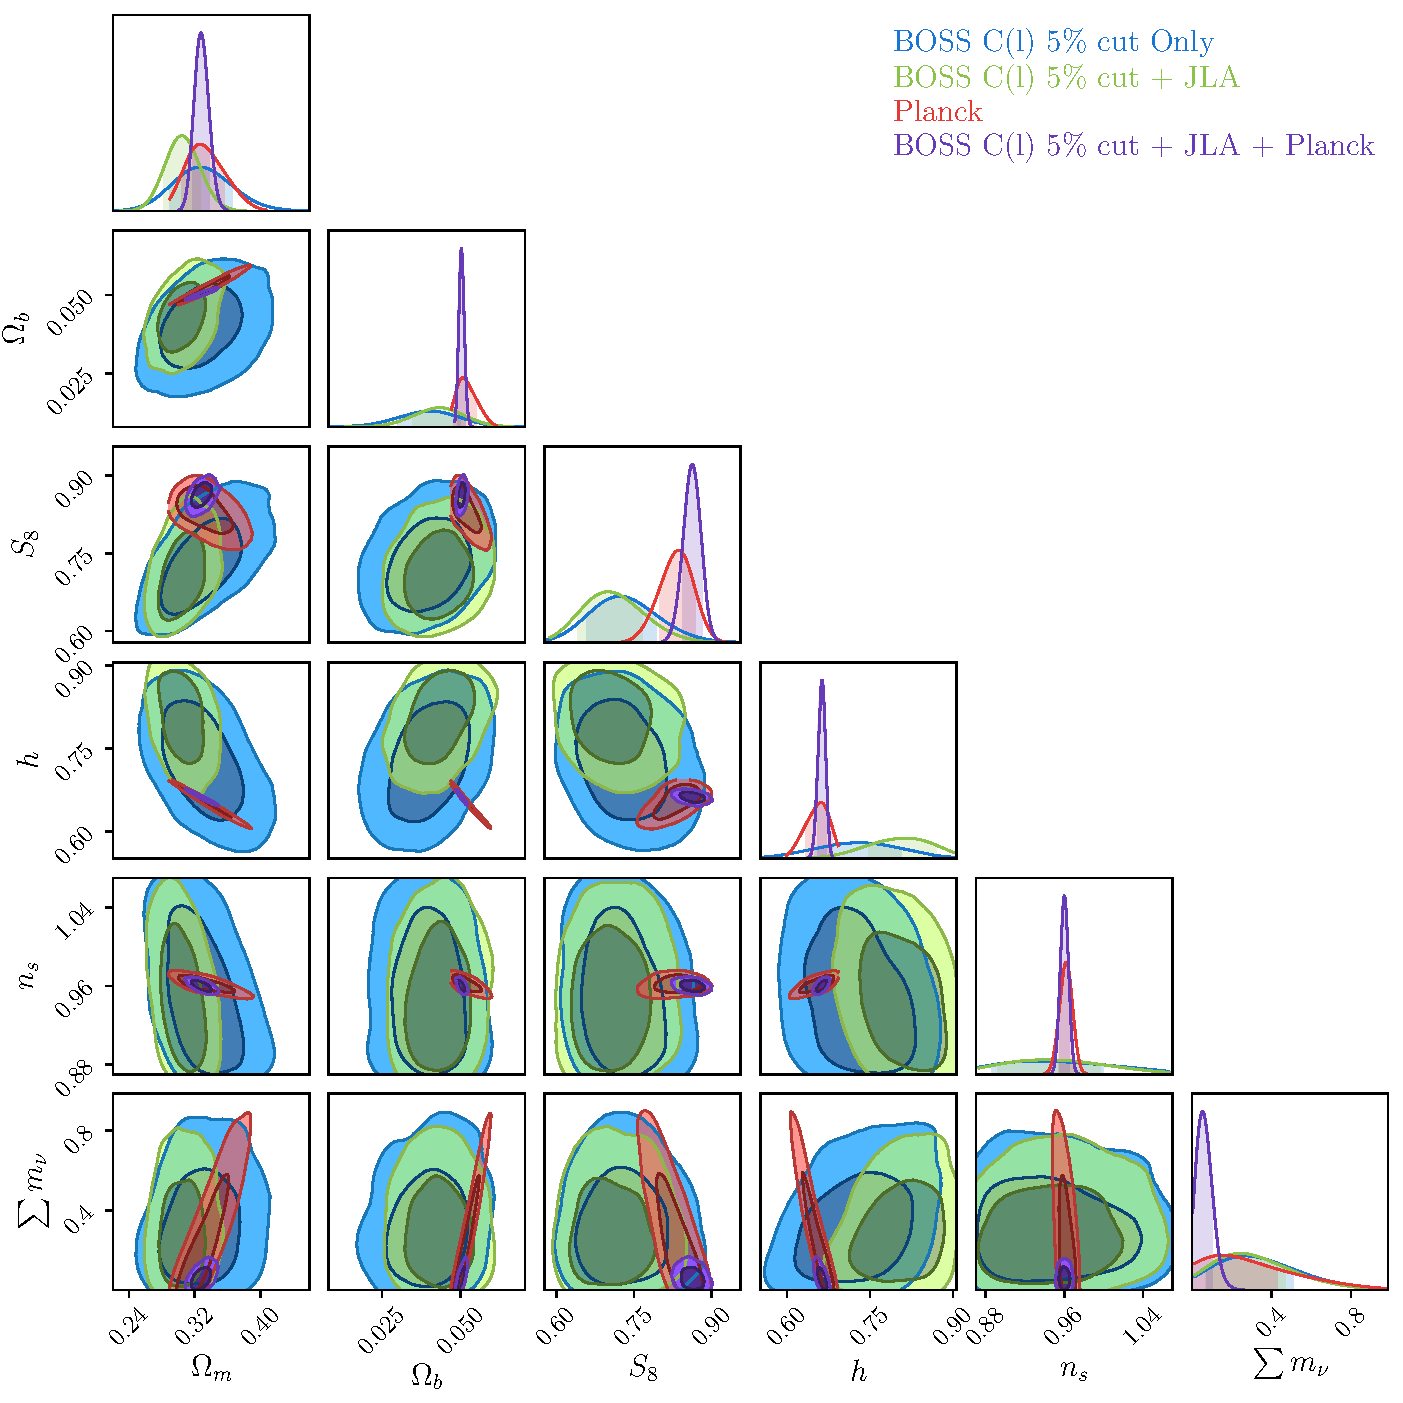
\includegraphics[width=\textwidth]{BOSS-FIGS/1Spec_Neutrino_NewPrior_LCDM_5pc.pdf}
\caption[1D and 2D marginalised credible intervals for a $\Lambda$CDM Cosmology with $\sum m_{\nu}$ when using scales up to $k_{max}\approx 0.07 h$ Mpc$^{-1}$]{1D and 2D marginalised credible intervals for a \textbf{$\Lambda$CDM Cosmology with $\sum m_{\nu}$} when using scales up to $k_{max}\approx 0.07 h$ Mpc$^{-1}$ ($\ell_{max}^{5\%}$ cut). Here I show the $\Omega_m$, $\Omega_b$, $S_8$, $h$, $n_s$, and $\sum m_{\nu}$ contours for BOSS $C_{\ell}$s alone \textit{(blue)}; BOSS $C_{\ell}$s plus JLA \textit{(green)}; Planck high-$\ell$ TT, TE, EE and low-$\ell$ P \textit{(red)}; and BOSS $C_{\ell}$s plus JLA and Planck high-$\ell$ TT, TE, EE and low-$\ell$ P \textit{(purple)}. As most of the scales that contain clean information on the neutrino masses are cut off, the 95\% CI upper bound found is $\sum m_{\nu} < 0.14$ eV.}
\label{fig:nuCDM5pc}
\end{center}
\end{figure}

\qquad Firstly, I perform an analysis using the same $\ell$-range as in the previous sections, $\ell_{max}^{5\%}$ from table \ref{Tb:EllCuts}. A summary for the marginalised 1D credible intervals from the cosmological estimation made with this cut can be found in the third part of table \ref{tab:LCDM_Constraints} showing the one sigma intervals for the $\Lambda$CDM parameters plus the 95\% upper limit for $\sum m_{\nu}$. The 1D and 2D marginalised credible intervals for this analysis can be found in Figure \ref{fig:nuCDM5pc}. When considering an approximation for the normal hierarchy, for a combination of BOSS $C_{\ell}$s, Planck CMB data, and supernovae data from JLA, the 95\% upper limit for sum of neutrino masses is:
\EQ{}{\sum m_{\nu} < 0.14 \, eV \quad \small\text{(BOSS + Planck + JLA -- $\ell_{max}^{5\%}$ cut)}}

\qquad From Figure \ref{fig:neutrinoCompare1} and even more so from Figure \ref{fig:neutrinoCompare2}, one can notice that this analysis is not so far from excluding zero total neutrino mass using cosmological data alone. As the power of such datasets increase it should be able, using the correct analysis and tools, to measure and detect neutrino masses independently from atmospheric experiments.

\qquad One more, I proceed to perform a consistency of datasets by using the evidence of each cosmological parameter estimation for these model to calculate the Bayes factor (Equation \ref{Eq:BayesFactor}). The following values, again, indicate the consistency of datasets for the considered model.
\begin{figure}
\begin{center}
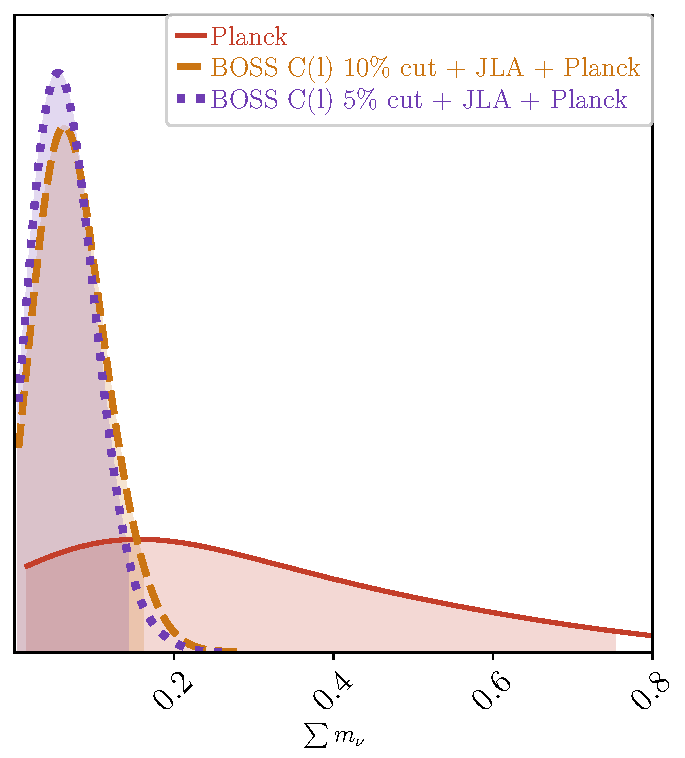
\includegraphics[scale=0.70]{BOSS-FIGS/neutrino_1D.pdf}
\caption[1D marginalised distribution with 95\% credible intervals for $\sum m_{\nu}$.]{1D marginalised distribution with 95\% credible intervals for $\sum m_{\nu}$ in three different cases: \textit{(red solid)} Planck high-$\ell$ TT, TE, EE and low-$\ell$ P, \textit{(yellow dashed)} BOSS $C_{\ell}$s with the $\ell_{max}^{10\%}$ cut plus Planck and JLA, and \textit{(purple dotted)} BOSS $C_{\ell}$s with the $\ell_{max}^{5\%}$ cut plus Planck and JLA. The 95\% upper limit for each case is, respectively: \textit{(red)} 0.76 eV, \textit{(yellow)} 0.16 eV, and \textit{(purple)} 0.14 eV.}
\label{fig:neutrinoCompare1}
\end{center}
\end{figure}
\begin{figure}
\begin{center}
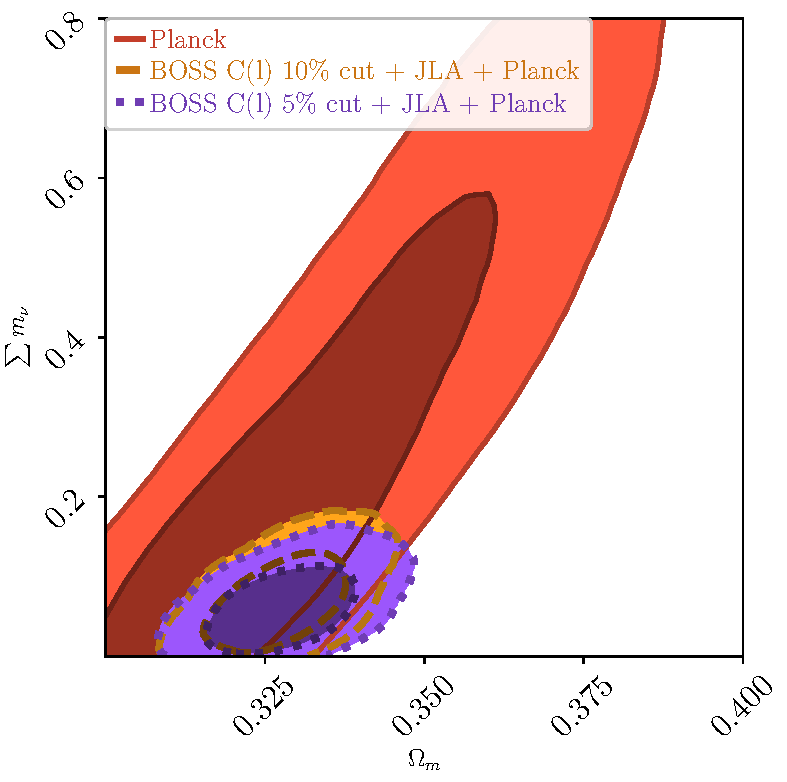
\includegraphics[scale=0.70]{BOSS-FIGS/neutrino_2D.pdf}
\caption[2D marginalised 1- and 2-$\sigma$ credible intervals for the $\sum m_{\nu}$-$\Omega_m$ plane.]{2D marginalised 1- and 2-$\sigma$ credible intervals for the $\sum m_{\nu}$-$\Omega_m$ plane for three different cases: \textit{(blue solid)} Planck high-$\ell$ TT, TE, EE and low-$\ell$ P, \textit{(red dashed)} BOSS $C_{\ell}$s with the $\ell_{max}^{10\%}$ cut plus Planck and JLA, and \textit{(orange dotted)} BOSS $C_{\ell}$s with the $\ell_{max}^{5\%}$ cut plus Planck and JLA.}
\label{fig:neutrinoCompare2}
\end{center}
\end{figure}

\begin{align}
R_{\scriptscriptstyle\text{BOSS+JLA}}^{\Lambda CDM + \sum m_{\nu} \, 5\%} & \simeq 1\times 10^2  \\
R_{\scriptscriptstyle\text{BOSS+PLANCK}}^{\Lambda CDM +\sum m_{\nu} \, 5\%} & \simeq 4\times 10^2 \\
R_{\scriptscriptstyle\text{PLANCK+JLA}}^{\Lambda CDM +\sum m_{\nu}} & \simeq 40 \\
R_{\scriptscriptstyle\text{BOSS+PLANCK+JLA}}^{\Lambda CDM +\sum m_{\nu} \, 5\%} & \simeq 3 \times 10^2
\end{align}
 

\qquad For the final analysis in this work, In want to investigate the impact of the chosen scale cuts in the neutrino mass upper bounds. To do it so, I extended the scales considered for the $\ell_{max}^{10\%}$ cuts (see table \ref{Tb:EllCuts} for details). This allows to access smaller scales that are still in the beginning of the so-called the weak non-linear regime \citep{Thomas2010Neutr,Bird2012}. Note that these scales are still larger than the scales that most collaborations use for power spectra or correlation function cosmological analysis \citep{Ho2012,2016BOSSCosmology,2017MNRAS.465.1454H,2017arXiv170801530D} -- \cite{2017arXiv170801530D}, for example, uses scales up to $0.78h$ Mpc $^{-1}$. In other words, one can be confident that the $\ell_{max}^{10\%}$ cuts are safe to be used, not using scales outside the weak non-linear regime. 


\qquad Using these second scale cuts, I then proceed to perform a similar cosmological analysis for a $\Lambda$CDM model with one massive species of neutrino, the approximation to the normal hierarchy. The 1D and 2D marginalised credible intervals for these final analysis can be find in Figure \ref{fig:nuCDM10pc} and the marginalised 68\% credible intervals for the $\Lambda$CDM parameters and the 95\% credible interval upper limit for $\sum m_{\nu}$ using this cut can be found in table \ref{tab:LCDM_Constraints}. The Bayes factors for this choice are shown below -- note that I have 2 further nuisance parameters in the $\ell_{max}^{10\%}$ cut as I checked that failure to add these reduces the Bayes factor significantly.
\begin{align}
R_{\scriptscriptstyle\text{BOSS+JLA}}^{\Lambda CDM + \sum m_{\nu} \, 10\%} & \simeq 70  \\
R_{\scriptscriptstyle\text{BOSS+PLANCK}}^{\Lambda CDM +\sum m_{\nu} \, 10\%} & \simeq 6 \times 10^2 \\
R_{\scriptscriptstyle\text{BOSS+PLANCK+JLA}}^{\Lambda CDM +\sum m_{\nu} \, 10\%} & \simeq 3 \times 10^5
\end{align}

\qquad This extended scale analysis demonstrates the robustness of the results presented in this section as the 95\% CI upper bound for $\sum m_{\nu}$ remains robust to these cuts (see Figures \ref{fig:neutrinoCompare1} and \ref{fig:neutrinoCompare2}):
\EQ{}{\sum m_{\nu} < 0.16 \, eV \quad \small\text{(BOSS + Planck + JLA -- $\ell_{max}^{10\%}$ cut)}.}



\begin{figure}
\begin{center}
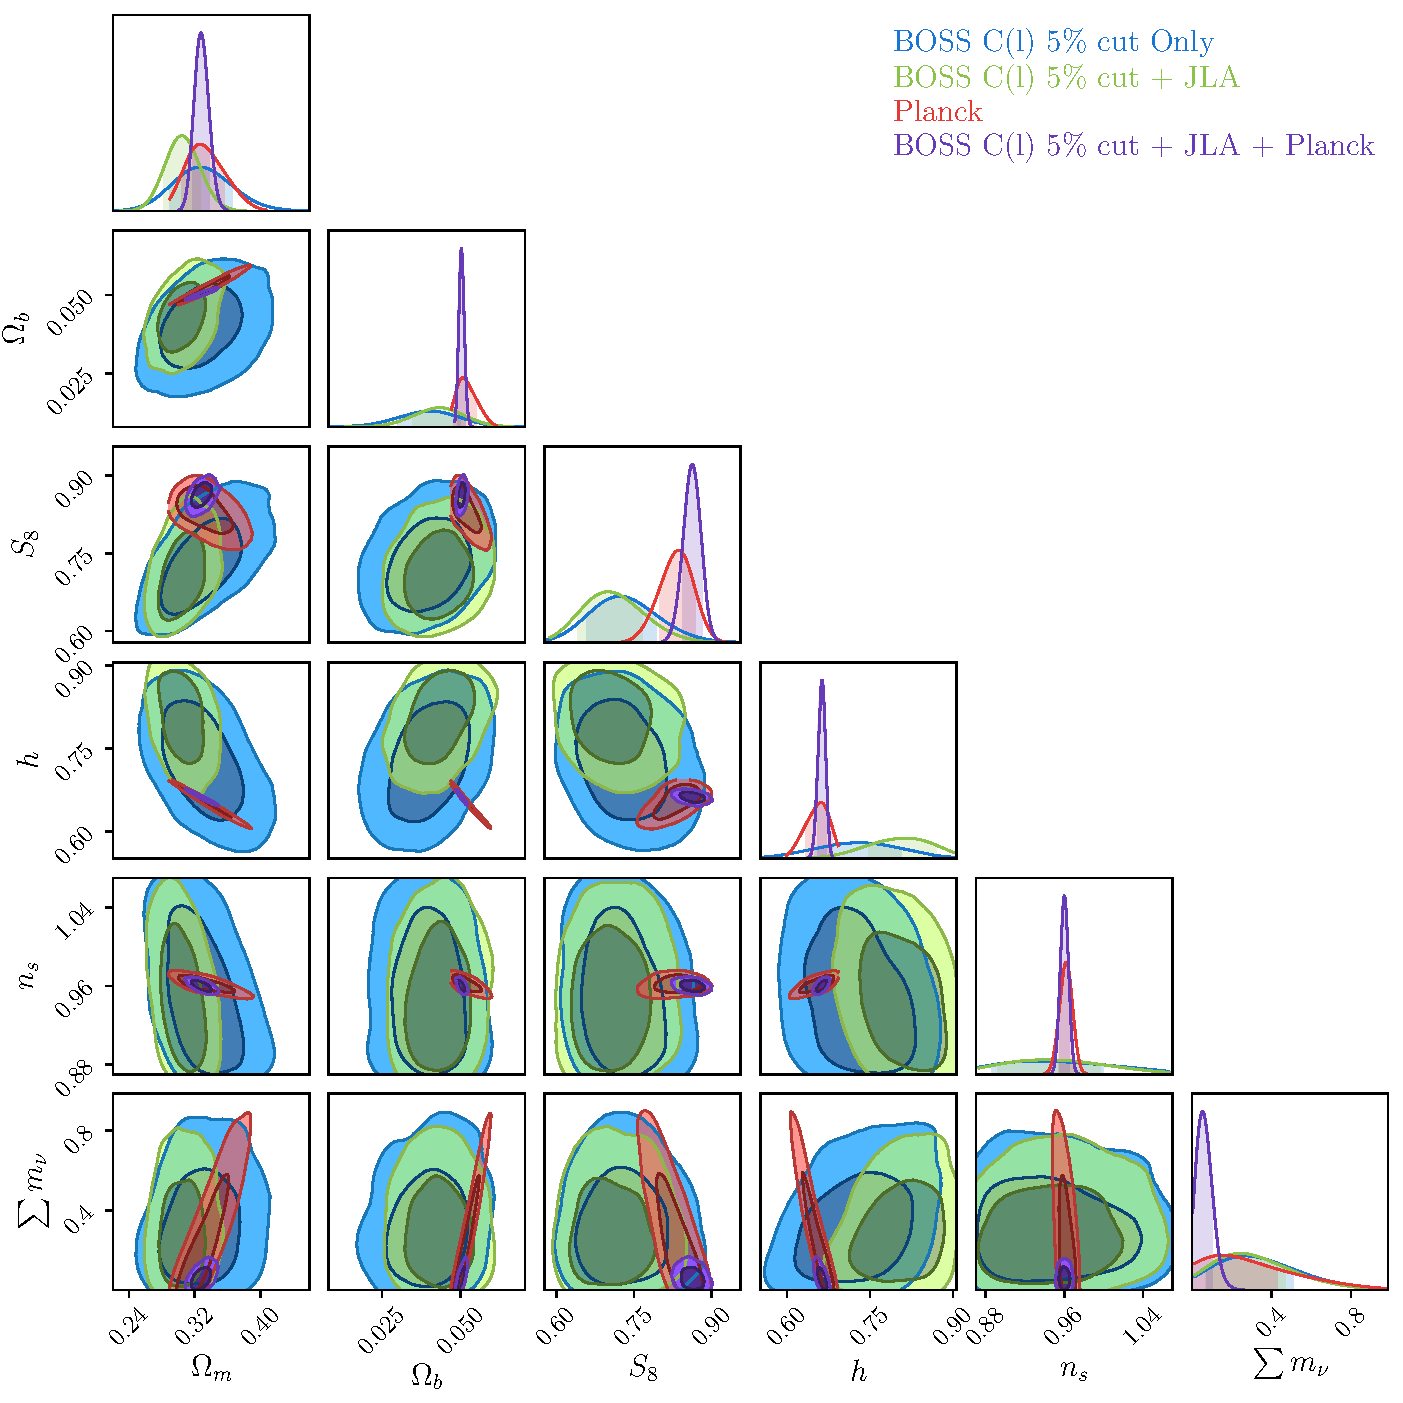
\includegraphics[width=\textwidth]{BOSS-FIGS/1Spec_Neutrino_NewPrior_LCDM_5pc.pdf}
\caption[Cosmological constraints for the $\Lambda$CDM + $\sum m_{\nu}$ model, using the $\ell_{max}^{10\%}$ cut]{Cosmological constraints for the \textbf{$\Lambda$CDM + $\sum m_{\nu}$ model}, using the $\ell_{max}^{10\%}$ cut, varying now six cosmological parameters, including the sum of neutrino masses considering only one massive species. This figure contains a combination of sampled and relevant derived parameters from the chains: $\Omega_m$, $\Omega_b$, $S_8$, $h$, $n_s$, and $\sum m_{\nu}$. Note that the Planck chains also varied $\tau_{reio}$. The \textit{blue contours} where estimated from the BOSS $C_{\ell}$s data alone using the SH16 likelihood; \textit{the green contours} are a combination the BOSS likelihood and JLA data; \textit{the red contours} are the Planck high-$\ell$ TT, TE, EE and low-$\ell$ P likelihood results; finally, the purple contours are a combination of the three probes: BOSS $C_{\ell}$, JLA and Planck (also high-$\ell$ TT, TE, EE and low-$\ell$ P). For this scale cut, the combination of datasets yields an upper bound on $\sum m_{\nu} < 0.16$eV.}
\label{fig:nuCDM10pc}
\end{center}
\end{figure}


\qquad A summary of all cosmological parameters estimated for all models and combinations of datasets can be found in table \ref{tab:LCDM_Constraints}.

%------------------------------------------------------------------------%
%                        CONCLUSIONS
%------------------------------------------------------------------------%
\section{Conclusions}
In this chapter, I produced several consistency checks which demonstrated the robustness of: the estimated covariance matrix, since the recovered cosmology was the same under different estimation methods (through simulation and theory); the likelihood, given it returns the same contours under three different approaches; and of the whole method, since I recovered the right cosmology using a controlled simulation.

\qquad Cosmological parameters were obtained for 3 different models: $\Lambda$CDM, $w$CDM, and $\Lambda$CDM with $\sum m_{\nu}$. I highlight the following main points regarding the results obtained in Section \ref{Sec:CosmoAnal}:
\begin{itemize}
\item[\textbf{1.}] The constraints obtained for all three models considered, using a tomographic analysis in harmonic space, are extremely competitive in comparison to the ones obtained by the BOSS Collaboration \citep{2016BOSSCosmology} and other recent big collaboration results such as DES \citep{2017arXiv170801530D} and KiDS \citep{2017MNRAS.465.1454H} with errors as small as the before-mentioned collaborations.

\item[\textbf{2.}] Even though information along the line-of-sight is ``washed away" due to projecting the data into tomographic bins, I obtain one of the tightest constraints for the  equation-of-state of dark energy with a $\sim$4\% error when combining BOSS $C_{\ell}$s, Planck CMB, and JLA Supernovae. This was never achieved before using $C_{\ell}$ with a spectroscopic survey and has constraints as tight as the one obtained from the state-of-the-art Dark Energy Collaboration analysis, using a combination of DES galaxy clustering \& weak lensing, Planck, JLA, and BAO \citep{2017arXiv170801530D}.

\item[\textbf{3.}] For the models and datasets considered, I find very high values for the Bayes factor, $R$, when combining BOSS $C_{\ell}$s, Planck, and JLA. I would like to highlight: $R_{\scriptscriptstyle\text{BOSS+PLANCK+JLA}} \simeq 4 \times 10^4$ for $\Lambda$CDM and $R_{\scriptscriptstyle\text{BOSS-10\%+PLANCK+JLA}} \simeq 3 \times 10^5$ for $\Lambda$CDM varying neutrino masses. 

\item[\textbf{4.}] The Bayes factor can also be used for model selection. Considering the combination of datasets, the Bayes factor between $\Lambda$CDM and $w$CDM is
\EQ{}{R_{w,\Lambda} = \frac{\mathcal{Z}(\vec{D}_{\text{BOSS+Planck+JLA}}|w\text{CDM})}{\mathcal{Z}(\vec{D}_{\text{BOSS+Planck+JLA}}|\Lambda\text{CDM})} = 0.67}
where $\vec{D}$ here just represents the overall combination of data vectors. This indicates that this combination prefers slightly more $\Lambda$CDM than $w$CDM, although no strong conclusion can be made. 

\item[\textbf{5.}] I find a small tension between BOSS $C_{\ell}$s and Planck for $S_8$ in all models considered with BOSS preferring smaller values. For example, for $\Lambda$CDM: 
\begin{align*}
S_8 & = 0.715^{+0.072}_{-0.064} \quad(\text{BOSS}) \\ \nonumber
S_8 &  = 0.850^{+0.023}_{-0.021}\quad(\text{Planck}) \nonumber
\end{align*}
although the combination of these datasets prefers higher values such as Planck (see table \ref{tab:LCDM_Constraints}) and the Bayes factor suggest the datasets are compatible. I conclude here that such tension can be investigated further with this method as LSS data increases in size and depth.

\item[\textbf{6.}] Although I do not show the contours in this chapter, I performed a cosmological analysis using a $\Lambda$CDM model but fixing $\sum m_{\nu} = 0 eV$ and compared with the $\Lambda$CDM results from Section \ref{Sec:LCDM}, which has a $\sum m_{\nu}$ fixed to $0.06$ eV. Using the Bayes factor for model selection, it is clear that the data prefers massive neutrinos against no neutrino mass at all:
\begin{align}
R_{0.06 eV, 0} & = \frac{\mathcal{Z}(\vec{D}_{\tiny\text{BOSS+Planck+JLA}}| \Lambda\text{CDM} + \sum m_{\nu} = 0.06)}{\mathcal{Z}(\vec{D}_{\tiny\text{BOSS+Planck+JLA}}| \Lambda\text{CDM} + \sum m_{\nu} = 0)} \nonumber \\
& = 8 \times 10^5 \nonumber
\end{align}

\item[\textbf{7.}] The neutrino mass constraints I obtain in this chapter can be compared to the tomographic analysis in real space done by \cite{2017SalazarBOSSwTheta}, which obtains an upper bound of $\sum m_{\nu} < 0.474$ eV (95\% CI). The reason I obtain much tighter constraints ($\sum m_{\nu} < 0.14$ eV (95\% CI)), even though I am also performing a tomographic analysis, is due to a series of decisions, including the approach I take to model the redshift dispersion and galaxy ``shell-crossing" (see Section \ref{Sec:SpecNz}), bias, and extra-shot noise. It is possible that the main difference between the results is due to different approach in modelling the neutrino mass hierarchy. In \cite{2017SalazarBOSSwTheta}, it is considered a model where the three neutrino species have degenerate mass hierarchy, i. e., the three masses are equal. This is already ruled out by particle physics experiments that measure the mass splitting from neutrino oscillation experiments (see \citealt{2014Gonzalez-GarciaNeutrino} for an update on the neutrino mass splitting fits). The approach I took in this chapter (see Section \ref{Sec:nCDM}) naturally yields smaller upper bounds in $\sum m_{\nu}$. In chapter \ref{Chap:Neutrinos}, I present a study about the impact of the model in the sum of neutrino masses and their hierarchy.

\end{itemize}


\begin{table}
    \centering 
    \caption[Marginalised cosmological constraints and 68\% credible intervals for the models considered in the BOSS analysis using a variety of datasets and combinations. ]{Marginalised cosmological constraints and 68\% credible intervals for the models considered in this work using a variety of datasets and combinations. The contours for these results are shown in Figures \ref{fig:LCDM_Cosmology} for $\Lambda$CDM, \ref{fig:wCDM_Cosmology} for $w$CDM, \ref{fig:nuCDM5pc} for the $\Lambda$CDM + $\sum m_{\nu}$ with $\ell^{5\%}_{max}$ cut, and \ref{fig:nuCDM10pc} for $\Lambda$CDM + $\sum m_{\nu}$ with $\ell_{max}^{10\%}$ cut.}
    \label{tab:LCDM_Constraints}
   \resizebox{\textwidth}{!}{
    \begin{tabular}{cccccc}
        \hline
        \hline\\[0.05cm]
		Model & Parameter & BOSS & BOSS & BOSS + JLA  & Planck \\
       & & & + JLA & + Planck & \\[0.05cm]
		\hline 
		\hline \\[0.05cm]
		$\Lambda$CDM & $\Omega_m$ & $0.315^{+0.034}_{-0.033}$ & $0.317^{+0.022}_{-0.021}$ & $ 0.327 \pm 0.008$ &  $0.315\pm 0.011$ \\[0.1cm] 
		& $\Omega_b$ & $0.0404^{+0.010}_{-0.009}$ & $0.0381^{+0.007}_{-0.008}$ & $0.0502 \pm 0.0006$ & $0.0492 \pm 0.0009$ \\[0.1cm]     
		& $S_8$ & $0.715^{+0.072}_{-0.064}$ & $0.745^{+0.059}_{-0.052}$ & $0.862^{+0.015}_{-0.016}$ & $0.850^{+0.023}_{-0.021}$ \\[0.1cm]      
		& $h$ & $0.716^{+0.088}_{-0.069}$ & $0.699\pm 0.039$ & $0.663 \pm 0.005$ & $0.672 \pm 0.008$ \\[0.1cm]      
		& $n_s$ & $0.929^{+0.064}_{-0.045}$ & $0.955^{+0.052}_{-0.048}$ & $0.960 \pm 0.004$ & $0.964 \pm 0.006$ \\[0.1cm]
		
        \hline \\[0.05cm]
        
      $w$CDM & $\Omega_m$ & $0.277^{+0.050}_{-0.042}$ & $0.308^{+0.021}_{-0.018}$  & $0.330 \pm 0.012$ & $0.213^{+0.062}_{-0.039}$\\[0.1cm]
		& $\Omega_b$ & $0.0318^{+0.0117}_{-0.0098}$ & $0.0429 \pm 0.007 $ & $0.0505 \pm 0.002$ & $0.0334^{+0.009}_{-0.006}$\\[0.1cm]      
		& $S_8$ & $0.726^{+0.072}_{-0.061}$ & $0.743^{+0.079}_{-0.068}$  & $0.863\pm 0.016$ & $0.811^{+0.037}_{-0.034}$\\[0.1cm]       
		& $h$ & $0.767^{+0.069}_{-0.091}$ & $0.745^{+0.049}_{-0.052}$ & $0.661\pm 0.012$ & $0.816^{+0.073}_{-0.101}$  \\[0.1cm]      
		& $n_s$ & $0.939^{+0.057}_{-0.049}$ & $0.957^{+0.049}_{-0.050}$ & $0.960 \pm 0.004$ & $ 0.964 \pm 0.006 $ \\[0.1cm]   
		& $w_0$ & $-1.36^{+0.36}_{-0.38}$ & $-1.030^{+0.073}_{-0.076}$ &  $-0.993^{+0.046}_{-0.043}$ & $-1.45^{+0.32}_{-0.23}$ \\[0.1cm]
        
       \hline\\[0.05cm]
       
      $\Lambda$CDM + $\sum m_{\nu}$ & $\Omega_m$ & $0.326^{+0.038}_{-0.035}$ & $0.304^{+0.022}_{-0.021}$ & $0.328 \pm 0.009$ & $0.326^{+0.028}_{-0.021}$\\[0.1cm]        
		[$\ell_{max}^{5\%}$ cut]& $\Omega_b$ & $0.040^{+0.009}_{-0.010} $ & $0.0432 \pm 0.008 $ & $0.05017^{+0.0009}_{-0.0008}$ & $0.0506^{+0.0039}_{-0.0026}$\\[0.1cm]      
		& $S_8$ & $0.723^{+0.069}_{-0.063}$  & $0.700^{+0.065}_{-0.056}$  & $0.862\pm 0.017$  & $0.836^{+0.031}_{-0.035}$\\[0.1cm]      
		& $h$ & $0.730^{+0.075}_{-0.078}$ & $0.814^{+0.054}_{-0.064}$ & $0.663^{+0.006}_{-0.007}$& $0.662^{+0.018}_{-0.026}$ \\[0.1cm]      
		& $n_s$ & $0.933^{+0.066}_{-0.046}$ & $0.941^{+0.055}_{-0.049}$ & $0.960 \pm 0.042$ & $ 0.962^{+0.006}_{-0.007} $ \\[0.1cm]      	 
       (95\% CI)[eV] & $\sum m_{\nu}$ & $ < 0.75 $ & $ < 0.71 $ &  $ < 0.14 $ & $ < 0.76 $ \\[0.1cm]
       
       \hline \\[0.05cm]
      $\Lambda$CDM + $\sum m_{\nu}$ & $\Omega_m$ & $0.345^{+0.033}_{-0.030}$ & $0.324^{+0.034}_{-0.029}$ & $0.333^{+0.014}_{-0.012}$ & $0.326^{+0.050}_{-0.029}$ \\[0.1cm] 
        
		[$\ell_{max}^{10\%}$ cut]& $\Omega_b$ &  $0.045 \pm 0.009$  & $0.040\pm 0.013$ & $ 0.0510^{+0.0016}_{-0.0014}$ & $0.0506^{+0.0069}_{-0.0033}$  \\[0.1cm] 
        
		& $S_8$ & $0.751^{+0.062}_{-0.057}$ & $0.768^{+0.097}_{-0.092}$ & $0.864^{+0.030}_{-0.029}$ & $0.839^{+0.058}_{-0.067}$  \\[0.1cm] 
        
		& $h$ &  $0.689^{+0.076}_{-0.066}$ & $0.661^{+0.067}_{-0.063}$ & $0.658^{+0.010}_{-0.011}$ & $0.662^{+0.024}_{-0.044}$ \\[0.1cm] 
        
		& $n_s$ & $0.930^{+0.062}_{-0.044}$ & $1.011^{+0.056}_{-0.086}$ &  $0.958 \pm 0.006$ & $0.962\pm 0.013$ \\[0.1cm]
		
        (95\% CI)[eV] & $\sum m_{\nu}$  & $>0.72$ & $< 0.66 $ &  $ < 0.16 $ & $ < 0.76 $ \\[0.1cm]
		\hline
		\hline
    \end{tabular}}
\end{table}








	% INCLUDE: system
% !TEX root = ../thesis-example.tex
%
\chapter{Neutrino Masses from Combined Cosmological Probes and Oscillation Experiments Constraints}
\label{Chap:Neutrinos}

\cleanchapterquote{You can’t crush ideas by suppressing them. You can only crush them by ignoring them. By refusing to think, refusing to change.}{Ursula K. Le Guin}{(The Dispossessed)}

\vspace*{\fill}

In this chapter, I investigate the impact of prior models on the upper bound of the sum of neutrino masses, \NM{}. I use a combination of datasets: Large Scale Structure of galaxies, Cosmic Microwave Background, Type Ia SuperNovae, and Big Bang Nucleosynthesis. I analyse physically motivated models (or exact models), which respect oscillation experiment constraints from particle physics, and compare them to constraints using standard cosmological approximations. The former give a consistent upper bound of $\sum m_{\nu} \lesssim 0.26$ eV (95\% CI) and yields a strong competitive upper bound for the lightest neutrino mass species, $m_0^{\nu} < 0.086$ eV (95\% CI). This is one of the first ever constraints set to the mass of the lightest neutrinos in the literature. By contrast one of the cosmological approximations, which is somewhat inconsistent with oscillation experiments, yields an upper bound of $\sum m_{\nu} \lesssim 0.15$ eV (95\% CI), which differs substantially from the former upper bound. I, therefore, argue that cosmological neutrino mass and hierarchy determination should be pursued using physically motivated models, taking into account knowledge from oscillation experiments, since approximations might lead to incorrect and nonphysical bounds.

\textit{The work in this chapter was presented in \citet{2018LoureiroNeutrinos}.} 

\newpage
\section{Introduction}
Particle physics experiments in the late 1990s, such as Super-Kamiokande \citep{Kamiokande1998}, and recent experiments, such as SNO \citep{2002SNO}, KamLAND \citep{2005KamLAND}, and others \citep{2008MINOS,2012RENOExperiment,AbeNeutrino2014}, have established the existence of massive neutrinos, taking a first step beyond the Standard Model of Particle Physics. The missing solar neutrino problem, an apparent discrepancy between the observed and predicted number of $\nu_e$ originated by the Sun, was solved by understanding that such particles change between the three known leptonian flavours: $\nu_e, \, \nu_{\mu}$, and $\nu_{\tau}$ \citep{2016Capozzi}. As the solar neutrino detector was sensitive only to the electron neutrino, $\nu_e$, fewer particles were detected due to neutrinos changing their \textit{flavours}. This oscillation between neutrino flavours implies that these particles have non-vanishing mass eigen-states, denoted: $m_1$, $m_2$, and $m_3$. 
%\andrei{This is andrei's comments}

\qquad Recent global fits to data from several neutrino oscillations experiments obtained constraints for two different mass squared splittings \citep{2014Gonzalez-GarciaNeutrino}; from solar neutrino experiments,
\begin{equation}
\Delta m_{21}^2 \equiv m_2^2 - m_1^2 \approx 7.49^{+0.19}_{-0.17} \times 10^{-5} \text{eV}^2\, ,
\end{equation}  

and from atmospheric neutrinos, 
\begin{equation}
|\Delta m_{31}^2| \equiv |m^2_3 - m_1^2| \approx 2.484^{+0.045}_{-0.048} \times 10^{-3} \text{eV}^2
\end{equation}

both with 1-$\sigma$ error-bars. These measurements imply that at least two of the neutrino mass-eigenstates are non-zero and, given that the sign of $\Delta m_{31}^2$ is unknown, that two scenarios are possible, related to the ordering of the masses: $m_1 < m_2 \ll m_3$, known as the \textit{normal hierarchy} (NH), or $m_3 \ll m_1 < m_2$, the \textit{inverted hierarchy} (IH). Current neutrino experiments will not be able to break the degeneracy between these two hierarchies (or orderings) in the near future \citep{2014Blennow}. However, by considering the lightest neutrino mass eigenstate to be zero one can see that these experiments set a lower bound for the sum of neutrino masses,  $\sum m_{\nu} \equiv \sum_{i=1}^3 m_{\nu, i}$, as follows:  $\sum m_{\nu}^{NH} > 0.0585 \pm 0.00048$ eV or $\sum m_{\nu}^{IH} > 0.0986 \pm 0.00085$ eV \citep{2016Hannestad,2018UpdateNeutrinoMass,2018LongNeutrinoMassPior}.
%Recent global fits to neutrino oscillations experiments data from Ref. \citep{2014Gonzalez-GarciaNeutrino} obtained constraints for two different mass squared splittings: from solar neutrino experiments, $\Delta m_{21}^2 \equiv m_2^2 - m_1^2 \approx 7.49^{+0.19}_{-0.17} \times 10^{-5}$ eV$^2$; and from atmospheric neutrinos, $|\Delta m_{31}|^2 \equiv |m^2_3 - m_1^2| \approx 2.484^{+0.045}_{-0.048} \times 10^{-3}$ eV$^2$ (1-$\sigma$ error-bars). These measurements imply that at least two of the neutrino mass-eigenstates are non-zero and, given that the sign of $\Delta m_{31}^2$ is unknown, two scenarios occur related to the ordering of the masses: $m_1 < m_2 \ll m_3$, known as \textit{the normal hierarchy} (NH); or $m_3 \ll m_1 < m_2$, known as the \textit{inverted hierarchy} (IH). Current neutrino oscillation experiments cannot break the degeneracy between these two hierarchies (or orderings) in the next following years \citep{2014Blennow}. However, from these experiments, a lower bound can be set for the sum of neutrino masses,  $\sum m_{\nu} \equiv \sum_{i=1}^3 m_{\nu, i}= m_1 + m_2 + m_3$, considering the lightest neutrino mass-eigenstate to be zero: $\sum m_{\nu}^{NH} > 0.0585 \pm 0.00048$ eV or $\sum m_{\nu}^{IH} > 0.0986 \pm 0.00085$ eV \citep{2016JCAP...11..035H,2018UpdateNeutrinoMass}.

\qquad From a different perspective, cosmological surveys have the potential to probe the sum of neutrino masses \citep{2007FBA,Thomas2010Neutr}, and also to constrain the neutrino mass hierarchy \citep{2003HannestadNeutrino,2016Hannestad}. The large scale structure of galaxies in the Universe is sensitive to the sum of neutrino masses and the number of massive neutrino species, $N_{\nu}$, since the cosmic energy density ratio for massive neutrinos in a $\Lambda$CDM model is

\begin{equation}
\label{Eq:NeutrinoOmega}
    \Omega_{\nu} = \sum_i^{N_{\nu}}\left[\left(\frac{G}{\pi^2H_0^2}\right)\int d^3p_i \frac{\sqrt[]{p_i^2 + m_{\nu,i}^2}}{(e^{p_i/T_{\nu,i}} + 1)} \right].
\end{equation} 

\noindent For the case of degenerate masses and after neutrinos start behaving non-relativistically, this can be approximated by \citep{Thomas2010Neutr}
\begin{equation}
    \Omega_{\nu} \approx \frac{\sum m_{\nu}}{(92.5\, h^2\text{eV})}\, .
\end{equation}
This approximation is at the core of the approach taken by most cosmological analyses when probing the related neutrino parameters; this leads to  95\% CI upper bounds on \NM{} as low as $< 0.12$ eV from Ly-$\alpha$ measurements \citep{2015LyAlpha-Deg} and also from the latest Planck Collaboration results \citep{2018PlanckCosmology}. A complete review of neutrino mass ordering in cosmology and particle physics can be found in \cite{2012Julien-Deg} and \cite{2018MassOrdering}.

\qquad In this chapter, I investigate the sensitivity of the angular power spectra of galaxies to massive neutrino parameters by analysing the impact such parameters have in the $C_{\ell}$s. Next, I present different ways to model the sum of neutrino masses in cosmology in order to analyse the impact of different classes of neutrino mass modelling strategies on cosmological parameters and neutrino constraints. This test is performed with the latest cosmological data, namely a tomographic analysis in harmonic space applied to the largest spectroscopic galaxy sample to date, the BOSS DR12 \citep[][-- also presented in Chapter \ref{Chap:BOSS}]{2018LoureiroBOSS}, combined with Planck cosmic microwave background (CMB) temperature, polarisation, and lensing \citep{PlanckCosmology2016}, Pantheon supernovae compilation data \citep{2018Pantheon}, BBN measurements of the deuterium-hydrogen fraction \citep{2018BBN-Measurements}, and, in some of the models, the latest neutrino mass squared splitting constraints from particle physics \citep{2014Gonzalez-GarciaNeutrino}.


\section{Neutrino Mass Effects in Harmonic Space}
\begin{figure}
\begin{center}
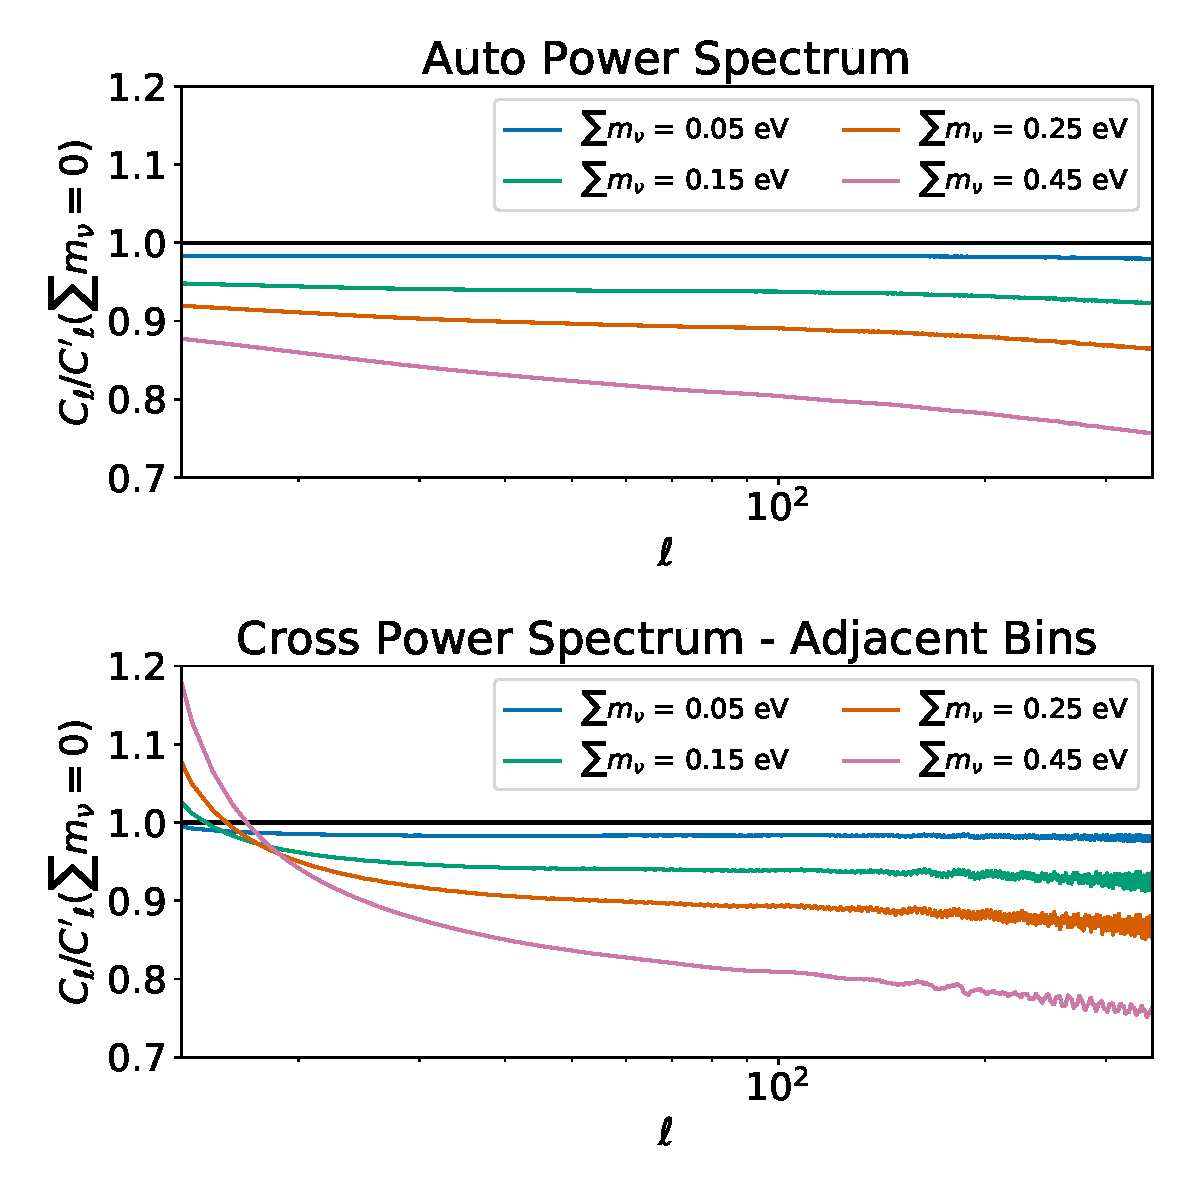
\includegraphics[scale=0.50]{Neutrino-FIGS/Neutrinos_SumMnu.pdf}
\caption[Impact of the sum of neutrino masses in the angular power spectra of galaxies.]{Impact of the sum of neutrino masses in the angular power spectra of BOSS galaxies shown as the ratio between $C_{\ell}$s calculated with different values of \NM{} over a case with no massive neutrinos, i.e. $\sum m_{\nu} = 0$ eV. \textit{(Top)} shows the ratio for the auto angular power spectra of a BOSS tomographic bin centred in $\bar{z} = 0.275$. \textit{(Bottom)} shows the ratio for the cross power spectrum between two BOSS bins, one centred in $\bar{z} = 0.275$ and its adjacent bin, $\bar{z} = 0.325$. Oscillations on the high-$\ell$ end of the spectrum are due to some numerical instabilities which do not affect the cosmological analysis due to band-width binning.}
\label{fig:neutrinoCompareSumM}
\end{center}
\end{figure}
Many works in the literature investigate the impact of massive neutrinos in the 3D power spectra or in the correlation function of galaxies \citep{2007FBA,2012Julien-Deg,Bird2012}. In a review \cite{2006NeutrinoReview}, it is shown how that for the 3D power spectrum of galaxies massive neutrinos suppress power after certain scales, $k \sim 5\times 10^{-3}$ h/Mpc; with a similar effect rising from the effective number of relativistic species, $N_{\text{eff}}$. The impact of massive neutrinos in the angular power spectra of galaxies is still to be explored as projection effects are so that it becomes unclear that the effect will be similar as that of the 3D power spectrum.

\qquad In this section, I make use of the \textit{Unified Cosmological Library for $C_{\ell}$s}, or \uclcl (Cuceu et al, \textit{in prep} -- benchmarked in Appendix \ref{Apx:Code_Comparison}), to generate theoretical predictions using a Planck-like fiducial cosmology\footnote{The fiducial $\Lambda$CDM cosmology used is $h=0.6725$, $\Omega_b = 0.0492$, $\Omega_{cdm} = 0.265$, $\ln 10^{10}A_s = 3.093$, $n_s = 0.965$, $\tau_r = 0.079$.} in order to investigate the impact of neutrino related parameters in the angular power spectra of galaxies. The objective of this study is to understand how sensitive the BOSS $C_{\ell}$s, presented in Chapter \ref{Chap:BOSS}, are to neutrino parameters. Therefore, I used the BOSS redshift distribution (as presented in Figure \ref{fig:NZ_BOSS}) and the same binning scheme as presented in Table \ref{Tb:Shells} to generate the theoretical $C_{\ell}$s; the bias and other nuisance parameters were kept to unity in order to simplify the analysis. For simplicity, figures displayed in this section show only an example of an auto power spectrum for a bin centred in $\bar{z} = 0.275$ and the cross power spectrum between this first bin and an adjacent one with $\bar{z} = 0.325$ -- both with $\Delta z = 0.05$.

\qquad There are three main parameters that will be considered in this section: the sum of neutrino masses, \NM{}, the effective number of relativistic species, $N_{\text{eff}}$, and the actual number of massive neutrinos, $N_{\nu}$.

\subsubsection{Impact of \NM{} in the galaxy angular power spectrum:}
In order to understand the impact of the sum of neutrino masses in the angular power spectra of galaxies, I kept the baryonic matter content of the Universe ($\Omega_b$) fixed as well as the curvature flat, i. e. $\Omega_{k} = 0$, meaning that $\sum_i \Omega_i = 1$. This implies that when varying the neutrino energy density via changing \NM{} (see Equation \ref{Eq:NeutrinoOmega}), $\Omega_{cdm}$ is not kept constant. Theoretical predictions were calculated for angular auto- and cross-power spectra between all BOSS redshift tomographic bins. Figure \ref{fig:neutrinoCompareSumM} shows an example of the ratio between different values of \NM{} against a case with no massive neutrinos for one auto- and one cross-power spectrum.

\qquad Differently from the usual 3D power spectrum analysis, it is clear from Figure \ref{fig:neutrinoCompareSumM} that massive neutrinos affect all scales (multipoles). This can only be explained by the fact that when performing a tomographic analysis, the radial scales get projected. The projection mixes the neutrino information (contained mostly in smaller scales for the 3D case) in a way that is now present in all multipoles. However, one must be careful when probing this parameter using $C_{\ell}$s from galaxy clustering. The more massive the total sum of neutrinos are, the more suppression of power occurs in all scales. From a different perspective, shot-noise also affects in the angular power spectra in all scales; however, the higher the shot-noise, the more increase of power in all scales is found. In Section \ref{Sec:nCDM}, it is pointed out how non-Poissonian (or extra) shot-noise, if not modelled correctly, could mimic low neutrino masses; Figure \ref{fig:neutrinoCompareSumM} confirms this statement. It is of fundamental importance to deal correctly with this effect. This becomes crucially important for spectroscopic galaxy surveys with very fine tomographic bins due to their small density of galaxies in each bin.

\subsubsection{Impact of $N_{\text{eff}}$ in the galaxy angular power spectrum:}
\begin{figure}
\begin{center}
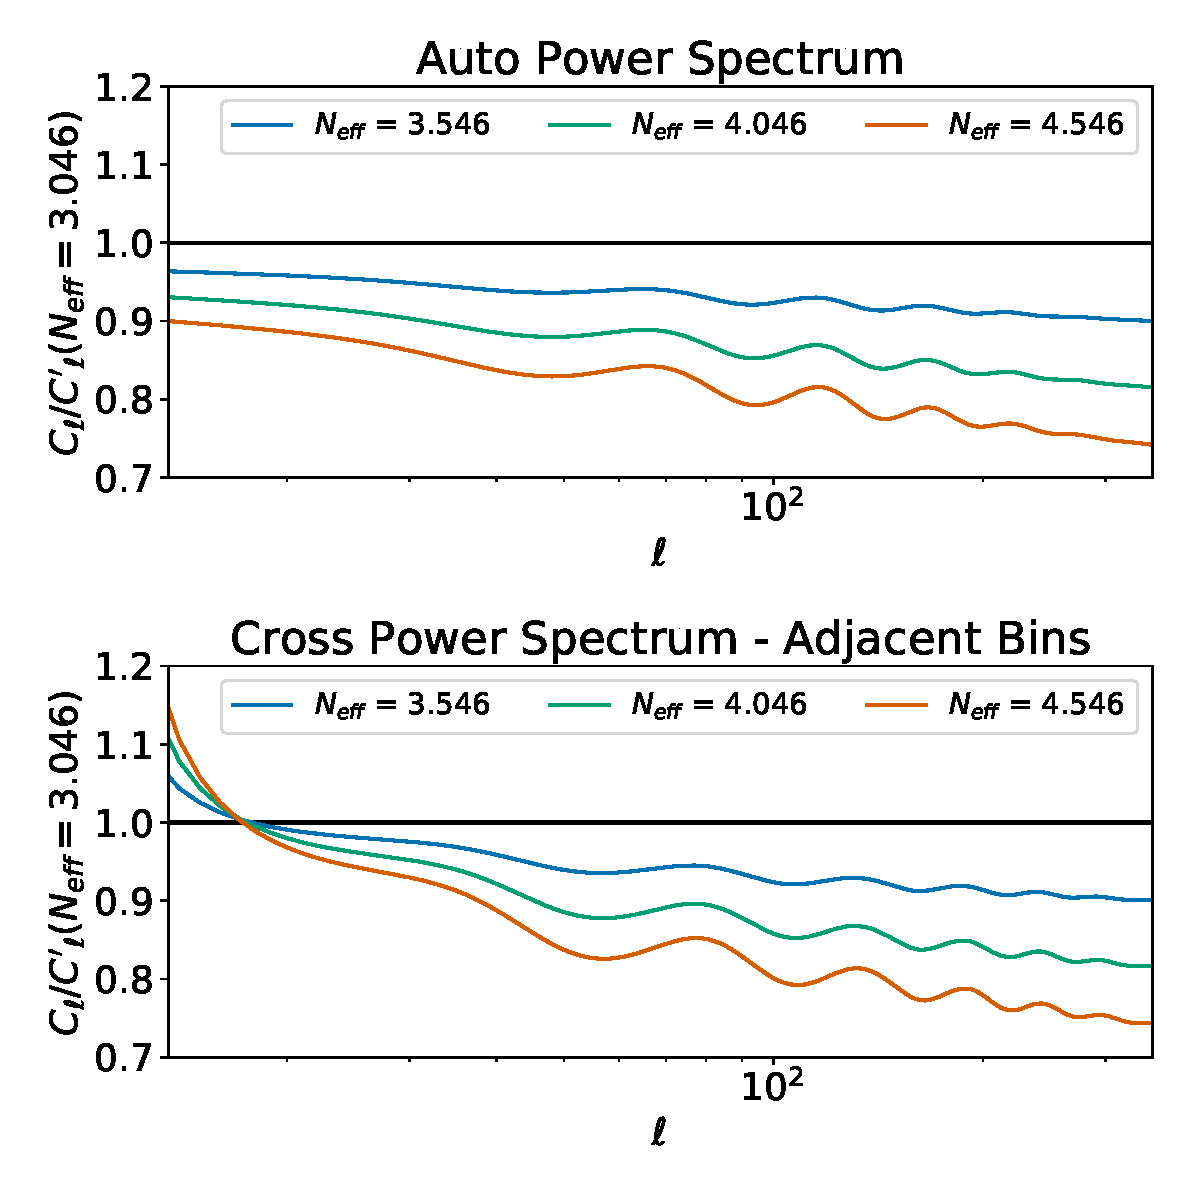
\includegraphics[scale=0.50]{Neutrino-FIGS/Neutrinos_Neff.pdf}
\caption[Impact of the effective number of relativistic species in the angular power spectra of galaxies.]{Ratio between $C_{\ell}$s with different values of $N_{\text{eff}}$ and $C_{\ell}$s containing $N_{\text{eff}} = 3.046$, the assumed fiducial value for $\Lambda$CDM. \textit{(Top)} Shows, as an example, the ratio between $C_{\ell}$ predictions for auto power spectrum of a BOSS tomographic bin with $\bar{z} = 0.275$. (Bottom) Same but for the cross power spectrum between adjacent bins centred in $\bar{z} = 0.275$ and $\bar{z} = 0.325$.}
\label{fig:neutrinoCompareNeff}
\end{center}
\end{figure}

The effective number of relativistic species is considered to be $N_{\text{eff}}\approx 3.046$. The reason this number not an integer is because it is also related to the temperature at which each massive neutrino species decouple from the other species and after the photon re-heating phase. Since not all neutrino species decouple at the same time, some species are still in thermal equilibrium with photons. As these photons get re-heated, some neutrinos will feel this effect, leading to a small excess of energy for this species. This can be dealt with by either probing each neutrino temperature separately with $N_{\text{eff}}=N_{\nu}$ or by considering $N_{\text{eff}}$ to be non-integer. The latter approach tends to be more efficient as it needs a much smaller parameter space.

\qquad From Figure \ref{fig:neutrinoCompareNeff}, one can see that, similarly to \NM, $N_{\text{eff}}$ affects all scales in the auto power spectrum of galaxies. However, the cross power spectrum demonstrates a different behaviour: for higher $N_{\text{eff}}$, higher is the increase of power for large scales while demonstrating a stronger suppression of power for small scales. A point of complete degeneracy can also be identified for small-$\ell$s. This different behaviour between angular auto- and cross-power spectra helps breaking some degeneracies when inferring cosmological parameters from this observational probe. If probing just the auto power spectra, the effect of $N_{\text{eff}}$ is similar to that of \NM{} and the shot-noise.

\subsubsection{Impact of $N_{\nu}$ in the galaxy angular power spectrum:}
\begin{figure}
\begin{center}
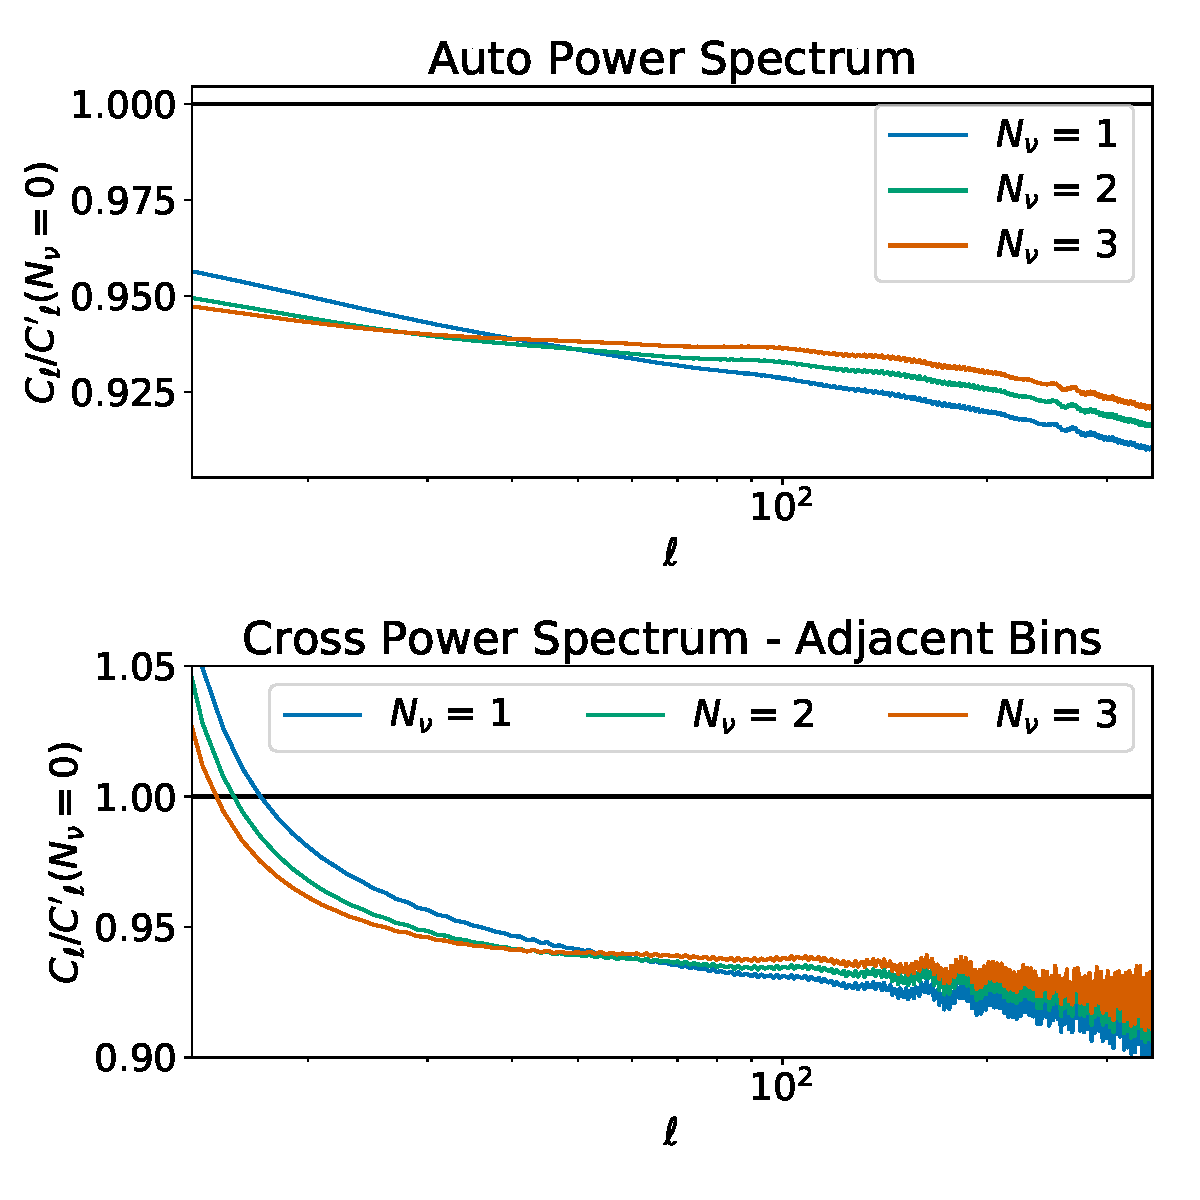
\includegraphics[scale=0.50]{Neutrino-FIGS/Neutrinos_Nnu.pdf}
\caption[Impact of the number massive neutrinos in the angular power spectra of galaxies.]{Ratio between $C_{\ell}$s with 1, 2 or 3 massive neutrinos against a case with no massive neutrino species. (Top) Ratio between the auto angular power spectra for different number of massive neutrinos for a redshift tomographic bin centred at $\bar{z} = 0.275$. (Bottom) Same ratio, now for the cross angular power spectra between adjacent bins centred at $\bar{z} = 0.275$ and $\bar{z} = 0.325$. Oscillations on the high-$\ell$ end of the spectrum are due to some numerical instabilities which are avoided using band-width binning in the cosmological analysis.}
\label{fig:neutrinoCompareNnu}
\end{center}
\end{figure}

From the three parameters related to neutrino properties analysed in this section, the number of massive neutrino species is the least sensitive of all when using clustering $C_{\ell}$s as a probe. Figure \ref{fig:neutrinoCompareNnu} shows that, although there is a significant difference between no massive neutrinos and $N_{\nu} > 0$, the difference between 1, 2 or 3 massive species is such that the current data considered in this work, the BOSS LSS sample, are not capable to distinguish between these scenarios when varying only this parameter. Even though the other parameters demonstrated a significant impact in the BOSS $C_{\ell}$s, the number of massive neutrino species is indistinguishable withing the estimated error-bars. This indicates the necessity of extra cosmological information from the CMB, SNe Ia, and BBN in order to probe all the considered neutrino mass properties.

\section{Neutrino Mass Models}

In this section, I describe the different neutrino models considered. These prior models are subdivided into two categories: exact models and cosmological approximations. The exact models incorporate particle physics constraints from neutrino oscillation experiments via modelling \NM{}, using a parametrisation based on the smallest neutrino mass, $m_0^{\nu}$ \citep{2012Hannestad,2016Hannestad,2018HeavensNeutrino}. For the normal hierarchy, one has:
\begin{align}
    \sum m_{\nu}^{NH} =\,  m^{\nu}_{0} & + \sqrt[]{\Delta m_{21}^2 + (m^{\nu}_{0})^2} + \sqrt[]{|\Delta m_{31}^2| + (m^{\nu}_{0})^2}
\end{align}
\noindent while in the inverted hierarchy: 
\begin{align}
    \sum m_{\nu}^{IH} =\,  m_0^{\nu} & + \sqrt[]{|\Delta m_{31}^2| + (m_0^{\nu})^2} + \sqrt[]{ |\Delta m_{31}^2| + \Delta m_{21}^2 + (m_0^{\nu})^2}.
\end{align} 
In what follows these will be referred to as the $m_0^{\nu}$-parametrisation. 

\qquad More explicitly, I consider four different exact models. \textit{Model 1} samples a binary switch parameter, $\mathcal{H}$, allowing the analysis to change between the two hierarchies with same prior volume, while also sampling the particle physics constraints for the mass splittings, $\Delta m_{21}^2$ and $|\Delta m_{31}^2|$, from Gaussian priors incorporating the errors in these measurements. \textit{Model 2} is similar to Model 1 but fixes the particle physics constraints to their central values: $\Delta m_{21}^2 = 7.49\times 10^{-5}$ eV$^2$ and $|\Delta m_{31}^2| = 2.484\times 10^{-3}$ eV$^2$. \textit{Model 3} (resp. \textit{Model 4}) fixes the mass splittings to their central values while also fixing the hierarchy to be normal (resp. inverted).

\qquad The second class of models, the cosmological approximations, are related to degenerated scenarios in which $\sum m_{\nu} = N_{\nu}\times m_{\text{eff}}$, where $m_{\text{eff}}$ is an effective mass, equal for each massive neutrino species. For each of these models, $N_{\nu}$ is fixed to a specific value and \NM{} is sampled. \textit{Model 5} is a NH approximation with $N_{\nu} = 1$, i.e., I approximate the two lower mass neutrino species to $m_1 = m_2 = 0$ \citep[][ -- also used in Chapter \ref{Chap:BOSS}]{2003HannestadNeutrino,2014Battye-Deg-1Mass,2016Giusarma-Deg-InvApp-NormAppr,PlanckCosmology2016,2018LoureiroBOSS}. Next, in a similar way, \textit{Model 6} is an IH approximation, where the lightest neutrino species is considered to be massless, which implies that $N_{\nu} = 2$ \citep{2016Giusarma-Deg-InvApp-NormAppr}. The last model in this class, \textit{Model 7}, is the most commonly used in standard cosmological analysis: the degenerate neutrino mass spectrum case, where $N_{\nu} = 3$ and $\sum m_{\nu} = 3m_{\text{eff}}$ \citep{2012Julien-Deg,2013Giusarma-Deg,2014Battye-Deg-1Mass,2015LyAlpha-Deg,2016Cuesta-Deg,2016BOSSCosmology,2016Giusarma-Deg-InvApp-NormAppr,2017Achidiacono-Deg,2017Cuchout-DegCase,2018PlanckCosmology,2017Vagnozzi-3deg,2018UpdateNeutrinoMass}. 

\qquad I also compared these seven models to cases where the \NM{} parameter is fixed to the most common values found in the literature for $\Lambda$CDM analysis \citep{2017arXiv170801530D,2017MNRAS.465.1454H,2018PlanckCosmology,2016BOSSCosmology}. \textit{Model 8} assumes no massive neutrinos; while \textit{Model 9} fixes it to the minimum possible value for the NH, $\sum m_{\nu} = 0.06$ eV, and sets $N_{\nu} = 3$ (as in the $\Lambda$CDM approach taken by the Planck Collaboration \citep{PlanckCosmology2016,PlanckResults2015}).

\qquad A summary of each model, together with the relevant neutrino mass parameters sampled %and the upper bounds for \NM{} and $m_{0}^{\nu}$ at 95\% credible interval (CI), 
can be found in Table \ref{Tb:Models1}.

\begin{table*}
  \centering
  \caption{A summary of the neutrino mass models considered in this chapter and the neutrino-related parameters sampled in each case.}
  \label{Tb:Models1}
  \begin{tabular}{cp{80mm}|c}
    \hline
    \hline
    Model & Description & $\nu$-Parameters\\[0.1cm]
    \hline
    \hline
    
     1 & Both hierarchies, $m_0^{\nu}$-parametrisation, sampling $|\Delta m_{31}^2|$ and $\Delta m_{21}^2$ from Gaussian priors. &  $m_0^{\nu}$, $\mathcal{H}$, $|\Delta m_{31}^2|$, $\Delta m_{21}^2$  \\
     
     2 & Both hierarchies,  $m_0^{\nu}$-parametrisation with $|\Delta m_{31}^2|$ and $\Delta m_{21}^2$ fixed to their central value. &  $m_0^{\nu}$, $\mathcal{H}$ \\
     
     3 & Normal Hierarchy,  $m_0^{\nu}$-parametrisation, fixed mass splittings. &  $m_0^{\nu}$ \\
     
     4 & Inverted Hierarchy,  $m_0^{\nu}$-parametrisation, fixed mass splittings. &  $m_0^{\nu}$ \\
     
     \hline
     5 & Normal Hierarchy approximation, $N_{\nu}=1$.  &  $\sum m_{\nu}$ \\
     
     6 & Inverted Hierarchy approximation, $N_{\nu}=2$. &  $\sum m_{\nu}$ \\
     
     7 & Degenerated masses approximation, $N_{\nu}=3$. & $\sum m_{\nu}$ \\
     \hline
     8 & No massive neutrinos, i.e., $N_{\nu}=0$ &   -- \\
     9 & Fixed to Normal Hierarchy's lower bound, $\sum m_{\nu} = 0.06$ eV &  -- \\
     \hline
     \hline 
  \end{tabular}
\end{table*}

\section{Assumptions}
\begin{table}
  \centering
  \caption{Ranges of priors used in all Bayesian analysis. All parameters sampled from flat priors with the exception of $\Delta m_{21}^2$ and $|\Delta m_{31}^2|$ which were sampled from Gaussians, $\mathcal{G}(\mu,\sigma)$. Parameters are divided into three groups: cosmological, neutrinos, and nuisance. Note that different models have different combinations of parameters.}
  \label{Tb:PriorsNeutrinos}
  \begin{tabular}{cc}
    \hline
    \hline
    Parameter & Prior Range \\
    \hline
    \hline
     $\Omega_b$ & $1 \times 10^{-3}, \, 0.3$    \\
     $\Omega_{cdm}$ & $0.0, \, 0.8$    \\[0.1cm]
     $\ln 10^{10} A_s$ & $2.0, \, 4.0$    \\
     $n_s$ & $0.87, \, 1.07$    \\
     $h$ & $0.55,\, 0.91$ \\
     $\tau^{Planck}_{reio}$  & $0.0,\, 0.8$ \\
     \hline
     $\sum m_{\nu}$ & $0.0,\, 1.0$ eV\\[0.1cm]
     $m^{\nu}_0$ & $1\times 10^{-4},\, 0.3$ eV \\
     $N_{\text{ur}}$ & $-N_{\nu},(6-N_{\nu})$ \\
     $\Delta m_{21}^2$ & $\mathcal{G}(\mu = 7.49, \sigma = 0.19)\times 10^{-5} eV^2$\\
     $|\Delta m_{31}^2|$ & $\mathcal{G}(\mu = 2.484, \sigma = 0.048)\times 10^{-3} eV^2$ \\
     \hline
     $b(z)$  & $1.1,\, 3.3$ \\
     $\sigma_s(z)$ & $1 \times 10^{-6},\, 9 \times 10^{-3}$ \\
     $\mathcal{N}_{11}$ & $0.0, \, 8\times 10^{-5}$ \\
     $\mathcal{N}_{12}$ & $0.0, \, 4\times 10^{-4}$ \\
     $y_{cal}^{Planck}$ & $0.99, \, 1.01$ \\
     $M_B^{SNe}$ & $-20.0,\, -18.5$\\
     \hline
     \hline
  \end{tabular}
\end{table}
Since the most recent analysis from the Planck Collaboration demonstrates that the Universe is flat to within 0.2\% precision, in this analysis I assume a flat $\Lambda$CDM scenario with massive neutrinos. The equation-of-state of dark energy is fixed to the cosmological constant case, $w=-1$. I also assume the possibility of extra effective ultra-relativistic particles, which are probed via the $N_{ur}$ parameter -- this parameter is degenerate with the decoupling of massive neutrinos at different temperatures and for simplicity I assume the same decoupling temperature. As the galaxy clustering information comes from BOSS DR12 angular power spectra, no fiducial cosmology was assumed for this sample (as explained in \cite{2018LoureiroBOSS} -- as well as in Chapter \ref{Chap:BOSS}). Priors for the standard $\Lambda$CDM parameters and nuisance parameters are described in Table \ref{Tb:PriorsNeutrinos} -- all priors were chosen to be flat, with the exception of the data-driven priors from neutrino oscillation experiments, $\Delta m_{21}^2$ and $|\Delta m_{31}^2|$, which are Gaussian priors. The priors were chosen based on previous works in the literature \citep{JLAdata,2016BOSSCosmology,PlanckCosmology2016,2017arXiv170801530D}, prioritising a trade-off between being physically motivated and being uninformative -- a more detailed discussion can be found in \ref{Sec:LikelihoodsPriors}. 

\qquad The neutrino related priors are $\sum m_{\nu} \in [0.0, 1.0]$ eV, $m_{0}^{\nu} \in [1\times 10^{-4},0.3]$ eV, and $N_{ur} \in [-N_{\nu},(6-N_{\nu})]$ for extra ultra-relativistic species or the temperature neutrinos decouple \citep{2012Julien-Deg}. This $N_{ur}$ dependency on $N_{\nu}$ for the extra ultra-relativistic species prior ensures an equivalent $N_{\text{eff}}$ prior on all models as $N_{\text{eff}}$ is a derived parameter in our analysis. For models sampling the hierarchy parameter, $\mathcal{H}$, the prior assigns equal odds for both hierarchies, i.e. the sampler uses a binary switch between both possibilities. Previous works in the literature like \cite{2017Simpson-Hier} have claimed to have found a `strong Bayesian evidence for the normal hierarchy'. Later on, it was demonstrated by \cite{2017-CommentSimpson} that this results were prior driven. By choosing flat probability distribution in logarithmic space for each of the individual neutrino masses, \cite{2017Simpson-Hier} accidentally favoured a normal hierarchy. In this work, such problem is avoided by sampling the hierarchy as an independent parameter. This ensures equal odd for both scenarios while avoiding biases from the prior choices.


\section{Data and Methodology}
The main galaxy sample used in this work is the BOSS DR12 large scale structure sample from \cite{BOSSCatalogue2016} as presented in \cite[][and in Chapter \ref{Chap:BOSS}]{2018LoureiroBOSS}. This sample is divided into 13 tomographic bins of $\Delta z = 0.05$ in a redshift range of $0.15 < z < 0.80$ containing around $\sim 1.15$M spectroscopic galaxies over more than 9,000 deg$^2$ in the sky. Angular power spectra of these galaxies are measured using a Pseudo-$C_{\ell}$ estimator (PCL) \citep[][ -- see Section \ref{Sec:Measurements}]{Thomas2011,Peebles1973,Efstat2004} in a bandwidth of $\Delta\ell =8$ \citep{2018LoureiroBOSS}. Covariances are calculated using 6,000 log-normal mocks with \texttt{FLASK} \citep{Flask2016} and a spline to the data's $C_{\ell}$s (to avoid introducing cosmological model assumptions). Due to the nature of the PCL estimator and partial sky observations, I forward model the mask effects into the likelihood, convolving theory with the mixing matrix, $S_{\ell} = \sum_{\ell'}R_{\ell \ell'} C_{\ell'}$. Other effects such as redshift space distortions, shell-crossing due to fingers-of-god (FoG), and extra Poissonian shot-noise are incorporated through the theoretical auto and cross-angular power spectra calculation. Detailed aspects related to the BOSS $C_{\ell}$ data vector, covariance matrix estimation, pipeline testing, and the implemented likelihood are outlined in Chapter \ref{Chap:BOSS}.

\qquad I combine the BOSS angular power spectra with external data from the cosmic microwave background, supernovae type Ia (SNe Ia), and big bang nucleosynthesis (BBN) at the likelihood level using the \textit{Unified Cosmological Library for Parameter Inference} code, or \texttt{UCLPI} (Cuceu et al., \textit{in prep.}), which uses the primordial power spectra and transfer function from \texttt{CLASS} \citep{Class}. The CMB data used is the 2015 Planck CMB temperature, polarisation and lensing measurements \citep{PlanckLikelihood2015}. The Planck likelihood uses low-$\ell$ modes for temperature (TT) and polarisation auto- and cross-correlations (BB, TB, EB). For higher multipoles, $\ell > 30$, I used temperature (TT) and polarisation auto- and cross-correlations (TE, EE) -- a configuration known as Planck TT,TE,EE+lowTEB \citep{PlanckLikelihood2015,PlanckResults2015}. The Planck lensing likelihood is also used, based on both temperature and polarisation maps. Next, I used  the most recent combined Pantheon SNe Ia sample \citep{2018Pantheon}. This sample contains 1,048 SNe Ia in a redshift range $0.01 < z < 2.3$ and contains data from Pan-STARRS, SDSS, SNLS and HST. The Big Bang Nucleosynthesis (BBN) information used in this work comes from measurements of the deuterium-hydrogen fraction estimated with recent improved helium-4 predictions as presented in \cite{2018BBN-Measurements}. The BBN likelihood was implemented with the help of the \texttt{AlterBBN} code \citep{2018AlterBBN}.  It was verified that the addition of BBN data does not have a direct impact on the neutrino mass parameters. BBN data help to constrain $N_{\text{eff}}$; better constraints on this parameter could have been achieved using extra BBN data such as He-4 (however, this is beyond the scope of this study).



\section{Analysis}
\begin{figure}
\begin{center}
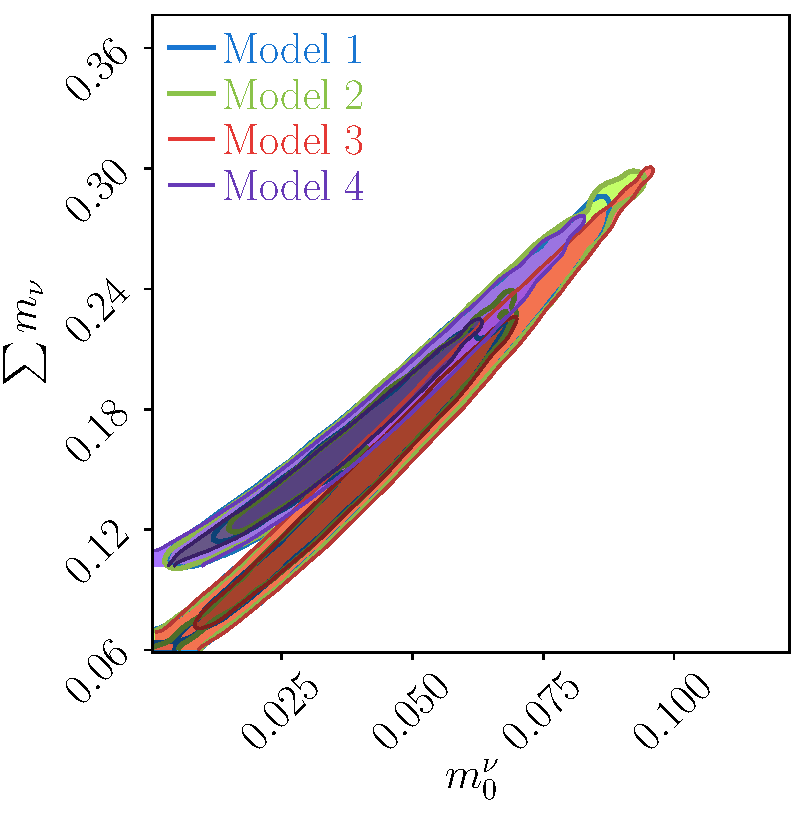
\includegraphics[scale=0.65]{Neutrino-FIGS/neutrino_hierarc_alt.pdf}
\caption[Two-dimensional (68\% and 95\% CI) marginalised posterior distributions for \NM{} and $m_0^{\nu}$ for the physically motivated models.]{Two-dimensional (68\% and 95\% CI) marginalised posterior distributions for \NM{} and $m_0^{\nu}$ for the physically motivated models, which take into account constraints from neutrino oscillation experiments. This panel shows that the current combination of cosmological data still do not have sufficient constraining power to differentiate between the two possible neutrino mass orders (or hierarchies).}
\label{fig:SumM0}
\end{center}
\end{figure}

 Nine different models were implemented to assess the impact of prior models on the upper bound of \NM{}. All models sample the basic $\Lambda$CDM parameters: $\{\Omega_b, \Omega_{cdm}, \ln 10^{10}A_s,$ $ n_s, h, \tau_{\text{reio}}\}$ as well as $N_{ur}$ to account for extra effective ultra-relativistic species. The posterior distribution analysis also contains several nuisance parameters for each of the datasets; these account for linear galaxy bias, $b(z)$, and redshift dispersion, $\sigma_s(z)$, for each of the 13 redshift tomographic bins in the BOSS dataset, two extra shot-noise parameters, $\mathcal{N}_{11}$ and  $\mathcal{N}_{12}$, for the last two bins in the BOSS dataset due to the lower number of galaxies in each of them, the absolute SNe Ia magnitude in the B-band for the Pantheon sample, $M_B^{SNe}$, and the overall Planck calibration nuisance parameter, $y_{cal}^{Planck}$. These result in a total of 30 nuisance parameters, all marginalised over after the posterior is sampled. I performed the analysis using two different nested samplers: \texttt{Multinest} \citep{2009Multinest} and \texttt{Pliny} \citep{PlinyRichardThesis}. The presented results are those from \texttt{Pliny}; the other sampler produced results that were essentially identical. %Priors for the basic $\Lambda$CDM, neutrinos, and nuisance parameters for this study are shown in Table \ref{Tb:PriorsNeutrinos}.
 
 
\qquad I performed a full cosmological analysis for all models using a combination of BOSS LSS $C_{\ell}$s, Planck CMB temperature and polarisation, Planck lensing, Type Ia SuperNovae from Pantheon, and BBN measurements of D/H data. The combination of datasets was performed at the likelihood level as described in Chapter \ref{Chap:BOSS-Cosmo}, Section \ref{Sec:CosmoAnal}. Figure \ref{fig:SumM0} shows the 2D marginalised constraints on \NM{} and $m_0^{\nu}$ for the exact models (Models 1-4). The marginalised one-dimensional posteriors for \NM{}, $N_{\text{eff}}$, and the lightest neutrino mass, $m_{0}^{\nu}$, for Models 1-7 can be found in Figure \ref{fig:neutrinoCompare1}, while the upper bounds can be found in Table \ref{Tb:Models}. The standard $\Lambda$CDM parameters, together with $N_{\text{eff}}$, are shown in Figure \ref{fig:LCDM} with the 1-$\sigma$ marginalised constraints summarised in Table \ref{tab:model_paramsLCDM}. An analysis of these results shows that all models essentially agree with each other in the $\Lambda$CDM and $N_{\text{eff}}$ parameters. Only a very small ($< 0.5 \sigma$) difference appears for the model with no massive neutrinos, Model 8, as shown in Figure \ref{fig:LCDM}.

\begin{table*}
  \centering
  \caption{Neutrino mass constraints for all models considered in this work with the 95\% CI upper bounds on both \NM, $m_{0}^{\nu}$, and $N_{\text{eff}}$. Results were obtained using a combination of BOSS $C_{\ell}$s, Planck CMB and lensing, SNe Ia from Pantheon, and BBN constraints. Models 1-4 also include constraints from oscillation experiments.}
  \label{Tb:Models}
  \begin{tabular}{c|ccc}
    \hline
    \hline
    Model & $\sum m_{\nu}$ & $m_0^{\nu}$ & $N_{\text{eff}}$\\
    & \small{[95\% CI]} & \small{[95\% CI]} & \small{[95\% CI]}\\[0.1cm]
    \hline
    \hline

     1 &  $< 0.264$ eV & $< 0.081$ eV & $3.18^{+0.38}_{-0.37}$\\
     2 & $<0.275$ eV & $< 0.086$ eV & $3.17^{+0.35}_{-0.33}$ \\
     3 &  $< 0.261$ eV & $< 0.085$ eV & $3.17^{+0.35}_{-0.33}$ \\
     4 &  $< 0.256$ & $< 0.078$ eV & $3.18\pm 0.34$ \\
     \hline
     5 & $< 0.154$ eV & -- & $3.15^{+0.35}_{-0.36}$ \\
     6 & $< 0.215$ eV & -- &  $3.16\pm 0.35$ \\
     7 & $< 0.270$ eV & -- & $3.17^{+0.38}_{-0.35}$ \\
     \hline
     8 & -- & -- & $3.14\pm 0.35$ \\
     9 & -- & -- & $3.14^{+0.35}_{-0.33}$ \\
     \hline
     \hline
  \end{tabular}
\end{table*}

%\RED{Should I check and mention something about nuisance params?}
\begin{figure}
\begin{center}
\includegraphics[width=\columnwidth]{Neutrino-FIGS/neutrino_prior_models.pdf}
\caption[Results for neutrino related parameters from the neutrino model prior analysis.]{The marginalised posterior probabilities for neutrino-related parameters for a range of neutrino models with 95\% CI shaded regions for neutrino parameters. Exact models (Models 1-4) yield  robust constraints for the upper bound of $\sum m_{\nu} \lesssim 0.26$ eV (95\% CI) and for the lightest neutrino mass $m_0^{\nu} \lesssim 0.086$ eV (95\% CI), while models with cosmological approximations (Models 5-7) have up to 43\% variation for the upper bound of $\sum m_{\nu}$ at 2-$\sigma$ CI. The vertical dashed line in the left plot shows the minimum possible value for $\sum m_{\nu}$ for the NH while the shaded region shows the same for the IH. All models also sample the $\Lambda$CDM parameters, shown in Figure \ref{fig:LCDM}. All results shown  were obtained by varying $N_{\text{eff}}$ and therefore present a wider, stronger statement than would have been the case for a fixed value of $N_{\text{eff}}$. }
\label{fig:neutrinoCompare1}
\end{center}
\vspace{-2.5mm}
\end{figure}
\qquad The marginalised posteriors for \NM{} (Figure \ref{fig:neutrinoCompare1}) show that the use of exact models yield robust upper bounds at 95\% CI, varying between $< 0.256$ eV and $<0.275$ eV. The models in which the hierarchy was also sampled, Models 1 and 2, did not demonstrate a significant choice between NH and IH; therefore, I marginalised over the hierarchy to get the results shown in Figure \ref{fig:neutrinoCompare1}. Meanwhile, the commonly used cosmological approximations demonstrate a variation in the 95\% CI upper bound of 43\% between Models 5 and 7: $\sum m_{\nu} < 0.154$ eV and $\sum m_{\nu} < 0.270$ eV, respectively. This indicates that such approximations can be problematic and that the upper bounds obtained are dominated by the prior model choice.

\qquad The nested sampler used in the cosmological analysis provides us with Bayesian evidences for each of the models. The ratio of evidences between two models, known as the Bayes factor, quantifies statistically if either is more strongly supported by the data \citep{1995BayesFactor}. The Bayes factors for all other pairs of models were consistent with one to within the statistical precision of the nested sampling algorithm, meaning that the data considered in this work do not strongly support any one of our models over the others.

\section{Conclusions}
\begin{figure}
\begin{center}
\includegraphics[width=\columnwidth]{Neutrino-FIGS/LCDM_Params_prl_alt.pdf}
\caption[One- (68\% CI) and two-dimensional (68\% and 95\% CI) marginalised posterior distributions for the relevant sampled and derived $\Lambda$CDM parameters in each of the nine different models.]{One- (68\% CI) and two-dimensional (68\% and 95\% CI) marginalised posterior distributions for the relevant sampled and derived $\Lambda$CDM parameters considered in each of the nine different models (where, $S_8 \equiv \sigma_8\sqrt{\Omega_m/0.3})$. All models agree in the basic $\Lambda$CDM parameters and for $N_{\text{eff}}$ to within half-$\sigma$ or less; Model 8 is an outlier among the models, since it contains no massive neutrinos, and hence often yields a mild outlier among the marginalised posterior distributions. This results address the issue of how the modelling of neutrinos should be done within a standard $\Lambda$CDM analysis where the \NM{} is not the main focus of the analysis. It is clear that the simpler approach, leading to no biases, is the one taken by Model 9 (same as in \cite{PlanckCosmology2016,2018PlanckCosmology}).  Finally, note that changing the neutrino mass modelling does not affect $N_{\text{eff}}$. This suggests that if one wishes to study $N_{\text{eff}}$, the particular model chosen for the neutrino masses does not seem to play a role.}
\label{fig:LCDM}
\end{center}
\end{figure}


In this chapter I have shown that the choice of how the neutrino is modelled for cosmological purposes significantly affects current upper bounds for the sum of the neutrino masses. If physically motivated exact models are chosen, the upper bound is found to be $\sum m_{\nu} < 0.264$ eV (95\% CI). On the other hand, we now possess enough cosmological data to show that this upper bound is significantly different if one makes the approximation that one (two) of the neutrino mass eigenstates have zero mass and that the mass is contained in the other two (one) eigenstates. 

\qquad Here, I show a concise framework, applied to the largest spectroscopic galaxy survey to date, to obtain robust neutrino mass information from a combination of cosmological observations and particle physics constraints. Even though no model was preferred from a Bayesian evidence analysis, cosmological approximations can cause a variation up to 44\% on the upper bound of \NM{}, while all exact models yield results that vary only by 7\% for the upper bound (both considered at 95\% CI). Using this exact modelling methodology, I present what it is believed to be one of the first cosmological measurement of the upper bound of the lightest neutrino mass species: $m_{0}^{\nu} < 0.086$ eV at 95\% CI. Even though the posterior distributions for $m_{0}^{\nu}$ in Figure \ref{fig:neutrinoCompare1} exhibits a peak, I do not claim it to be a detection as Bayes factor analysis between models were inconclusive and zero is still within the 95\% CI.

\qquad In light of these results, I argue that the approach presented here as Model 1 should be the choice for current and future cosmological neutrino mass investigations (given the volume of data now available to cosmologists). One should no longer make approximations assuming a degenerate neutrino mass spectrum as this could lead to potentially nonphysical upper bounds and constraints. Instead, one should make use of a cosmological analysis that takes into account both of the neutrino mass hierarchies, as well as particle physics constraints and their uncertainties. 

\qquad Finally, I demonstrated here that, if neutrino masses are not the interest of the analysis, the simplest model which fixes the sum of neutrino masses to the particle physics lower bound for the NH, $\sum m_{\nu} = 0.06$ eV, yields reliable cosmological results in the $\Lambda$CDM model context. In other words, a standard $\Lambda$CDM analysis is independent of the fiducial choice for the neutrino mass model, allowing for a simple approach to be taken. I emphasise that one should consider massive neutrinos for a standard $\Lambda$CDM analysis -- as the data is sensitive enough, as seen in the difference between the model with zero massive neutrinos (Model 8) and all others in Figure \ref{fig:LCDM}. The exact approach for neutrino mass estimation will be extremely relevant for future cosmological neutrino studies in the analysis of the next generation of surveys, e. g. DESI \citep{2016-DESI}, Euclid \citep{2011EuclidRedPaper}, LSST \citep{LSST}, and J-PAS \citep{JPAS}.


\begin{landscape}
\begin{table}
    \centering
    \caption[Marginalised $\Lambda$CDM parameters constraints and 68\% credible intervals for all 9 models considered.]{Marginalised $\Lambda$CDM parameters constraints and 68\% credible intervals for all 9 models considered. All constraints were obtained from a combination of BOSS LSS $C_{\ell}$s, Planck CMB temperature and polarisation, Planck lensing, Type Ia SuperNovae from Pantheon, and BBN measurements of D/H data}
    \label{tab:model_paramsLCDM}
    {\begin{tabular}{c|ccccccc}
        \hline
        \hline
		Model & $\Omega_m$ & $\Omega_b$ & $n_s$ & $h$ & $S_8$ & $\tau_{r}$ & $N_{\text{eff}}$\\ 
		\hline
		\hline
	1 & $0.327\pm 0.011$ & $\left( 49.8^{+1.8}_{-1.7} \right) \times 10^{-3}$ & $\left( 966.1^{+7.5}_{-7.7} \right) \times 10^{-3}$ & $0.667\pm 0.014$ & $0.837^{+0.011}_{-0.012}$ & $0.058\pm 0.014$ & $3.18\pm 0.19$ \\ 
		2 & $\left( 327.3^{+9.8}_{-9.6} \right) \times 10^{-3}$ & $\left( 50.0\pm 1.6 \right) \times 10^{-3}$ & $\left( 965.7^{+7.2}_{-6.8} \right) \times 10^{-3}$ & $0.666\pm 0.013$ & $0.837\pm 0.011$ & $0.059^{+0.013}_{-0.014}$ & $3.17^{+0.18}_{-0.17}$ \\ 
		3 & $\left( 326.9^{+9.1}_{-9.2} \right) \times 10^{-3}$ & $\left( 49.9^{+1.5}_{-1.6} \right) \times 10^{-3}$ & $\left( 965.4^{+7.1}_{-6.5} \right) \times 10^{-3}$ & $0.667\pm 0.012$ & $0.838^{+0.012}_{-0.011}$ & $0.058\pm 0.014$ & $3.17^{+0.18}_{-0.17}$ \\ 
		4 & $\left( 328.0^{+9.2}_{-9.5} \right) \times 10^{-3}$ & $\left( 50.0^{+1.6}_{-1.5} \right) \times 10^{-3}$ & $\left( 965.7^{+7.2}_{-7.0} \right) \times 10^{-3}$ & $0.666^{+0.013}_{-0.012}$ & $0.838\pm 0.011$ & $0.058\pm 0.013$ & $3.18^{+0.17}_{-0.18}$ \\ 
		5 & $\left( 321.8^{+9.3}_{-9.0} \right) \times 10^{-3}$ & $\left( 49.1^{+1.6}_{-1.5} \right) \times 10^{-3}$ & $\left( 964.5\pm 6.8 \right) \times 10^{-3}$ & $0.671\pm 0.013$ & $0.842\pm 0.011$ & $0.050\pm 0.012$ & $3.15\pm 0.18$ \\ 
		6 & $\left( 323.3^{+10.3}_{-9.3} \right) \times 10^{-3}$ & $\left( 49.4^{+1.7}_{-1.5} \right) \times 10^{-3}$ & $\left( 965.2^{+7.0}_{-7.3} \right) \times 10^{-3}$ & $0.670\pm 0.013$ & $0.840\pm 0.011$ & $0.053\pm 0.014$ & $3.16^{+0.18}_{-0.17}$ \\ 
		7 & $0.325\pm 0.010$ & $\left( 49.7\pm 1.7 \right) \times 10^{-3}$ & $\left( 965.6^{+7.3}_{-7.2} \right) \times 10^{-3}$ & $0.668^{+0.014}_{-0.013}$ & $0.838^{+0.012}_{-0.011}$ & $0.057^{+0.014}_{-0.015}$ & $3.17^{+0.19}_{-0.18}$ \\ 
		8 & $\left( 316.2^{+9.2}_{-9.1} \right) \times 10^{-3}$ & $\left( 48.3^{+1.6}_{-1.5} \right) \times 10^{-3}$ & $\left( 964.6^{+7.4}_{-7.7} \right) \times 10^{-3}$ & $0.677\pm 0.013$ & $0.845\pm 0.011$ & $0.045^{+0.013}_{-0.014}$ & $3.14\pm 0.18$ \\ 
		9 & $\left( 319.3^{+9.2}_{-8.7} \right) \times 10^{-3}$ & $\left( 48.9^{+1.6}_{-1.5} \right) \times 10^{-3}$ & $\left( 964.7\pm 7.1 \right) \times 10^{-3}$ & $0.673\pm 0.013$ & $0.842\pm 0.011$ & $0.049\pm 0.013$ & $3.14^{+0.18}_{-0.17}$ \\ 
		\hline
		\hline
    \end{tabular}}
\end{table}
\end{landscape}
 % INCLUDE: concepts
% !TEX root = ../thesis-example.tex
%
\chapter[An investigation of Bayesian-$C_{\ell}$ Estimators applied to Galaxy Clustering]{An investigation of Bayesian Angular Power Spectra Estimators applied to Galaxy Clustering}\label{Chap:BPL}
%\chapter{}\label{sec:concepts}

\cleanchapterquote{It's f*cking science!\\
Just ask Albert Einstein, he invented space
}{Danny Sexbang}{(Dinosaur Laser Fight, Ninja Sex Party)}



In this section, I present the investigation for applications of a fully Bayesian methodology to generally estimate angular power spectra from data distributed on a sphere. It provides tools for optimal power spectrum estimation of to CMB temperature, CMB polarisation modes, galaxy clustering, weak lensing convergence ($\kappa$), cosmic shear ($\gamma_1$ \& $\gamma_2$), and cross-correlations of all previous probes. In other words, this estimator works for any spin-0 fields, spin-2 fields, and cross-correlations; however, it has never been tested in the context of galaxy surveys. The method makes use of a Guided Hamiltonian Sampling, a variant of the usual Hamiltonian Sampling, to sample from the spherical harmonics coefficients,$a_{lm}$, and the angular power spectra, $C_{\ell}$. The final marginalised $C_{\ell}$'s provides covariance matrices and uncertainties with no the need of simulated mocks due to the sampling nature of the problem. I applied this method to partial and full-sky Euclid-like Log-Normal simulations and compared the results with a Pseudo Power Spectrum estimator.
\RED{Improve here. What is the main point?}

\section{Introduction}
\RED{Talk once more on LCDM and how we can go beyond it...}
With a plethora of new cosmological observations in the horizon, there is an increasing necessity in the field for the use of an unified framework to combine different probes. Surveys like DESI, Euclid, COrE, LSST, J-PAS \RED{CITE ALL} would directly benefit from combining Cosmic Microwave Background, galaxy clustering, and galaxy lensing observations. 
%With a plethora of new cosmological observations in the horizon -- like  -- there is an increasing necessity for an unified framework to combine various cosmological probes.  such as CMB, galaxy clustering, and galaxy lensing. 
Recent studies have demonstrated the power of probing cosmological parameters using 3x2-point statistics (using galaxy clustering, galaxy lensing and cross-correlations of both) or 5x2-point (CMB polarisation, galaxy clustering, galaxy lensing and cross-correlations) statistics data vectors \cite{DES and Niccola}. 
\begin{itemize}
\item Talk more about DES
\item Different estimators: MQL, PCL and their disadvantages
\item Talk about the importance for small-$\ell$ -- $f_{nl}$
\item No need for mocks
\item Euclid case
\end{itemize}

\section{Bayesian Approach to Measure the Angular Power Spectra}\label{Sec:BPL:Modeling}
In this section, I will establish the formalism towards expressing a generic Bayesian modelling for angular power spectra estimation for data distributed on a sphere. The formalism developed here can be applied to CMB temperature data ($T$), CMB polarisation data($\Theta_P$), galaxy clustering ($\delta_g$), and probes of weak gravitational lensing like cosmic shear ($\gamma$) and convergence ($\kappa$). As a natural extension of the generic method, this also applies to cross-correlations between all of the above observables. In other terms, this Bayesian method for $C_{\ell}$ estimation works for spin-0 and spin-2 fields, considering also cross-power spectra between these.

\qquad Section \ref{Sec:BPL:Spin-0_Form}, starts by developing a general formalism for spin-0 fields like galaxy overdensities, weak lensing convergence, and CMB temperature (based on a previous work by \cite{Taylor2008}). We then move to the Bayesian inference modelling of measuring angular power spectra for such fields. Next, on Section \ref{Sec:BPL:Spin-2_Form}, we extend this formalism for Spin-2 fields like CMB polarisation and weak lensing shear, finishing this Section with a formalism for the Bayesian inference of Spin-0 and Spin-2 angular power spectra estimation.


%--------------------------------------------------------------%
%                  SPIN-1 MODELLING
%--------------------------------------------------------------%
\subsection{Spin Zero Fields}\label{Sec:BPL:Spin-0_Form}
One may start the modelling by partitioning the sky into pixelised regions of equal area, $x_p$. For an underlying cosmological field, measurements can be described by a vector -- e.g. $T(x_p)$ for CMB temperature or $\delta_g (x_p)$ for galaxy overdensities. Let $\mathbf{\Theta} \equiv \Theta(\mathbf{x}_p)$ denote a general spin-0 data vector which can be represented in harmonic space in terms of the coefficients of a spherical harmonic expansion:

\begin{equation}
\Theta (\mathbf{x}_p) = \sum_{\ell=0}^{\ell_{max}}\sum_{m=-\ell}^{\ell}a_{\ell m}Y_{\ell m}(\mathbf{x}_p).
\label{Eq:Spin0Decomp}
\end{equation}
\noindent this basis, the measured signal in the sky can be decomposed in an underlying signal vector, $\mathbf{s}$, and a noise vector, $\mathbf{n}$; in a way that the data can now be written as $\mathbf{d=s+n}$. The measured signal and the underlying spin-0 field are related via a linear mapping that takes into account any observational effects like instrumental pointing, masking, and beam effects: $\mathbf{s = R\Theta}$. Following, the spherical harmonics formalism, the relation between signal and noise can be re-written with the use of Equation \eqref{Eq:Spin0Decomp} as
\begin{align}
\mathbf{d=RYa+n}\, ,
\label{Eq:DataDecomposed}
\end{align}
\noindent  where $\mathbf{Y} \equiv Y_{\ell m}(\textbf{x}_p)$ are the spherical harmonics eigen-functions of the Laplace-Beltrami operator \citep{2008DahlenSimons}, $\mathbf{a} \equiv a_{\ell m}$ are the spherical harmonics coefficients which obey the relation $a_{\ell m} = (-1)^{m}a^*_{\ell (-m)}$. Note that the noise is also represented in this basis as $\textbf{n} \equiv n_{\ell m}$. 

\qquad In this context, the spin-0 fields are assumed to be isotropic Gaussian random fields with zero mean, i.e, $\langle \textbf{a} \rangle = \langle \textbf{n} \rangle = 0$, and covariances can be defined as

\begin{align}
\label{Eq:DataCov} \mathbf{C} & \equiv \langle \textbf{a} \textbf{a}^T \rangle = C_{\ell}\delta_{\ell \ell'}\delta_{m m'}, \\ 
\label{Eq:NoiseCov} \mathbf{N} & \equiv \langle \textbf{n} \textbf{n}^T \rangle = N_{\ell}\delta_{\ell \ell'}\delta_{m m'} \, , 
\end{align}
\noindent for the signal and the noise respectively. In Equation \eqref{Eq:DataCov}, the set of coefficients $\{C_{\ell}\}$ define the angular power spectrum of spin-0 fields. More generally, let $C_{\ell}^{ij, pq}$ denote the cross-power spectrum where \textit{(i,j)} are redshift tomographic bins and \textit{(p,q)} are probes. \footnote{In what follows, however, I will suppress the notational dependence on \textit{i,\, j,\, p}, and \textit{q}.} Equally, $N_{\ell}$ in Equation \eqref{Eq:NoiseCov} is defined as the noise power spectrum. Finally, the data covariance can be expressed as a sum of the two above covariances

\begin{equation}
\textbf{D} = \textbf{C} + \textbf{N} \, .
\end{equation}

\subsubsection{Bayesian inference for spin-0 fields:}
\qquad Now, the formalism is sufficient so one can take a Bayesian approach to infer the angular power spectra of spin-0 fields using sampling techniques. This approach can be formulated as the posterior probability of obtaining the $\{C_{\ell}\}$ given the data vector, $\mathbf{d}$:

\begin{align}
\Pr (\{C_{\ell}\}|\mathbf{d}) \propto \mathcal{L} (\mathbf{d}|\{C_{\ell}\})\Pi(\{C_{\ell}\}).
\label{Eq:LikelFirstExpression}
\end{align}
\noindent where $\mathcal{L} (\mathbf{d}|\{C_{\ell}\})$ is the likelihood of the data given the true $\{C_{\ell}\}$ and $\Pi(\{C_{\ell}\})$ is a prior in the angular power spectra. In a first approach, the expression above becomes a Maximum Likelihood estimation \citep{1994Gorsky,1997Tegmark,Hobson2002,Efstat2004} if one sets the prior probability distribution function on the angular power spectrum to $\Pi(\{C_{\ell}\}) = 1$. 

\qquad Following \cite{Borrill1999,Hobson2002,Taylor2008}, as both signal and noise are assumed to have a Gaussian nature, one can write the likelihood of the data as
\begin{align}
\mathcal{L}(\mathbf{d}|\{C_{l}\}) = \frac{1}{(2\pi)^{N_d/2}|\mathbf{D}|^{1/2}}\exp \left(-\frac{1}{2}\mathbf{d}^T\mathbf{D}^{-1}\mathbf{d} \right)\, .
\label{Eq:LikelihoodSpin0}
\end{align}

\qquad The right hand side of Equation \eqref{Eq:LikelihoodSpin0} can be estimated in reasonable computational time for very low resolution data. As the data's resolution increases, the dimensionality of the data covariance matrix $\mathbf{D}$, and hence its storage and memory requirements, increase drastically. This method becomes extremely complicated to deal with due to expensive inversion of $\mathbf{D}^{-1}$ following by the calculation of its determinant. Therefore, for the resolutions I am aiming in this work, the likelihood estimation in equation \eqref{Eq:LikelihoodSpin0} becomes extremely expensive\footnote{It is possible to find methods that work around this matrix inversion problem, but the matrix size makes the linear algebra an extremely complicated task}. 

\qquad To overcome this issue, two possible roads can be taken regarding two different approaches. The first one is to approximate the likelihood, in some way, to avoid the one given by equation \eqref{Eq:LikelihoodSpin0}. These methods are far from being optimal and can bias the likelihood. A second approach would be to estimate the signal realisation full posterior distribution and the angular power spectrum using Monte Carlo techniques \citep{Taylor2008,AlmostBlackPearl2016}. The $\{ C_{\ell}\}$ coefficients can be estimated with a marginalisation over all signal realisations sampled in the posterior. 

\qquad The power spectra's posterior distribution can be simply obtained from sampling from the joint distribution of $\{C_{\ell}\}$ coefficients and the signal realisation, $\Pr(\{C_{\ell}\},\mathbf{a}|\mathbf{d})$, and marginalising over the spherical harmonic coefficients \citep{Eriksen2004,Wandelt2004,Taylor2008,AlmostBlackPearl2016}:
%\qquad Now, following the approach described by \cite{Eriksen2004}, \cite{Wandelt2004}, \cite{Taylor2008}, and \cite{AlmostBlackPearl2016}, the posterior distribution of the power spectrum, $\Pr (\{C_{\ell}\}|\mathbf{d})$, can be obtained by sampling from the joint distribution of power spectrum coefficients and signal realisation, $\Pr(\{C_{\ell}\},\mathbf{a}|\mathbf{d})$, and finally marginalising over the $\mathbf{a}$ coefficients:
%\RED{CHANGE THE ABOVE PARAGRAPH!!!}

\begin{align}
\Pr(\{C_{\ell}\}|\mathbf{d}) = \int\Pr(\{C_{\ell}\},\mathbf{a}|\mathbf{d})\text{d}\mathbf{a}.
\label{Eq:LikelihInt}
\end{align}
\noindent The integrand can be expanded using Bayes theorem,

\begin{align}
\Pr(\{C_{\ell}\},\mathbf{a}|\mathbf{d}) \propto \mathcal{L}(\mathbf{d}|\mathbf{a})\mathcal{L}(\mathbf{a}|\{C_{\ell}\})\Pi(\{C_{\ell}\}). 
\label{Eq:Posterior1}
\end{align}
\noindent Given the assumed Gaussian nature of the noise, one can express $\mathcal{L}(\mathbf{d}|\mathbf{a})$ with the aid of Equation \eqref{Eq:DataDecomposed}:
\begin{align}
\mathcal{L}(\mathbf{d}|\mathbf{a}) \propto \exp \left[ -\frac{1}{2} (\mathbf{d-RYa})^T \mathbf{N}^{-1}(\mathbf{d-RYa}) \right] .
\end{align}
\noindent Furthermore, since the signal is also Gaussian,

\begin{align}
\mathcal{L}(\mathbf{a}|\{C_{\ell}\}) \propto \frac{1}{\sqrt{|\mathbf{C}|}}\exp\left( -\frac{1}{2} \mathbf{a}^T\mathbf{C}^{-1}\mathbf{a}\right).
\end{align}
\noindent With use of Equation \eqref{Eq:DataCov} the expression above can the re-written as:

\begin{align}
\mathcal{L}(\mathbf{a}|\{C_{\ell}\}) \propto \prod_{{\ell}=2}^{{\ell}_{max}}\left(\frac{1}{C_{\ell}}\right)^{(2\ell+1)/2} \exp \left[ -\frac{(2\ell+1)}{2}\frac{\sigma_\ell}{C_{\ell}}\right]\, ,
\end{align}
\noindent with 
\begin{align}
\sigma_{\ell} = \frac{1}{2\ell+1}\sum_m|a_{\ell m}|^2 \, ,
\end{align}
\noindent being the power spectrum of the signal realisation.

\qquad Finally, two components now express the posterior distribution: an Inverse-Gamma signal likelihood, and a Gaussian noise likelihood. Assuming that the noise in pixel space is uncorrelated, the noise covariance matrix, $\mathbf{N}$, will be diagonal. Furthermore, the signal's covariance matrix, $\mathbf{C}$, given by Equation \eqref{Eq:DataCov} is now diagonal in harmonic space. In this space, the likelihood $ \mathcal{L}(\mathbf{d}|\mathbf{a} )$ can be computed in an easier way. In other words, estimating the full posterior in the integrand of Equation \eqref{Eq:LikelihInt} becomes a much simpler task than calculating the full posterior in the left hand side of Equations \eqref{Eq:LikelFirstExpression} and \eqref{Eq:LikelihoodSpin0}. This is the usual approach taken by most works in the literature about Bayesian $C_{\ell}$ estimators.


%--------------------------------------------------------------%
%                  SPIN-2 MODELLING
%--------------------------------------------------------------%
\subsection{Spin Two Fields}\label{Sec:BPL:Spin-2_Form}
This section extends the formalism developed in the previous section to spin-2 fields like CMB polarisation and cosmic shear. Spin-2 fields can be separated into two independent modes related to the Stokes parameters. The first one is a curl-free mode, related to even-parity solutions, known as the E-mode; the second mode, related to odd-parity solutions, is the B-mode. In the formalism discussed in this Chapter, it is fundamental to note that incomplete sky coverage introduces mixing of these E- and B-modes, requiring the estimator to optimally deal with such systematic effects. In this section, I will adopt the same formalism and notation as in many seminal papers in the literature, as in \cite{Seljak1997}, \cite{Taylor2008} and \cite{Hikage2011}.

\qquad Starting with the argument that spin-2 fields are linear, they can fully be described by a traceless $2 \times 2$ tensor using only two of the Stokes parameters, $Q$ and $U$. The third Stokes parameter is related to the spin-0 field from Equation \eqref{Eq:Spin0Decomp}; while the fourth and final parameter is assumed to be zero since there's no circular polarisation generated by Thompson scattering (in the CMB context) and it is well known that there's no circular polarisation arising from the lensing potential (in the weak lensing context) \RED{Citation needed}. In the case for CMB polarisation, the two Stokes parameters, $U$ and $Q$, are related to the $2\times 2$ intensity tensor, $I_{ij}$, as $Q=(I_{11}-I_{22})/4$ and $U=I_{12}/2$; while in the context of weak lensing shear, this relation simply translates into the two shear components, $Q=\gamma_1$ and $U=\gamma_2$.

\qquad The three non-vanishing Stokes parameters can now be defined by an orthonormal directional vector, $\hat{\mathbf{n}}$, with respect to spherical coordinates. These can be expanded using a spin-2 spherical harmonic basis, $_{\pm 2}Y_{\ell m}(\hat{\mathbf{n}})$, as 
\begin{align}
\label{eqn::chCmbPol_stokes_paras}
\Theta(\hat{\mathbf{n}}) &= \sum_{\ell m}a_{\ell m}\,Y_{\ell m}(\hat{\mathbf{n}}) \\
\left[ Q(\hat{\mathbf{n}})\pm iU(\hat{\mathbf{n}}) \right] &= \sum_{\ell m}\left(E_{\ell m}\pm iB_{\ell m} \right)\,_{\pm 2}Y_{\ell m}(\hat{\mathbf{n}})\, ,
\end{align}
%\left[ Q(\hat{\mathbf{n}})\pm iU(\hat{\mathbf{n}}) \right] &= \sum_{\ell m}a_{\pm 2,\ell m}\,_{\pm 2}Y_{\ell m}(\hat{\mathbf{n}})\, ,
%\noindent where the coefficients $a_{\pm 2,\ell m}$ can be related to the E- and B-modes coefficients $a_{\ell m}^E$ and $a_{\ell m}^B$ through
\noindent where the harmonic coefficients of the E- and B-modes can be estimated directly from the shear/polarisation fields via the $Q$ and $U$ Stokes parameters \citep{PolSpice2005,Hikage2011},
\begin{align}
E_{\ell m} & = \frac{1}{2}\oint d\Omega_{\hat{\mathbf{n}}} \left[ Q(\hat{\mathbf{n}}) + iU(\hat{\mathbf{n}}) \right]\,_2Y^*_{\ell m} + \left[ Q(\hat{\mathbf{n}}) - iU(\hat{\mathbf{n}}) \right]\,_{-2}Y^*_{\ell m} \, ,\\
B_{\ell m} & = -\frac{i}{2}\oint d\Omega_{\hat{\mathbf{n}}} \left[ Q(\hat{\mathbf{n}}) + iU(\hat{\mathbf{n}}) \right]\,_2Y^*_{\ell m} - \left[ Q(\hat{\mathbf{n}}) - iU(\hat{\mathbf{n}}) \right]\,_{-2}Y^*_{\ell m}\, .
\end{align}

\qquad The covariances between the spherical harmonics coefficients, also referred as the angular power spectra, are given by

\begin{align}
\label{eqn::chCmbPol_psTT}
\textbf{C}^{\Theta,\Theta}  \equiv & \langle a_{\ell m}^{*} a_{\ell'm'} \rangle  = C_{\ell}^{\Theta\Theta}\delta_{\ell\ell'}\delta_{mm'},\\
\label{eqn::chCmbPol_psEE}
\textbf{C}^{E,E} \equiv & \langle E_{\ell m}^{*} E_{\ell'm'} \rangle = C_{\ell}^{EE}\delta_{\ell\ell'}\delta_{mm'},\\
\label{eqn::chCmbPol_psBB}
\textbf{C}^{B,B} \equiv &\langle B_{lm}^{*} B_{l'm'} \rangle = C_{\ell}^{BB}\delta_{\ell\ell'}\delta_{mm'},\\
\label{eqn::chCmbPol_psTE}
\textbf{C}^{\Theta,E} \equiv & \langle a_{\ell m}^{*} E_{\ell'm'} \rangle = C_{\ell}^{\Theta E}\delta_{\ell\ell'}\delta_{mm'}, \\
\textbf{C}^{\Theta,B} \equiv &\langle a_{lm}^{*} B_{l'm'} \rangle = C_{\ell}^{\Theta B}\delta_{\ell\ell'}\delta_{mm'},\\
\textbf{C}^{E,B} \equiv &\langle E_{lm}^{*} B_{l'm'} \rangle = C_{\ell}^{EB}\delta_{\ell\ell'}\delta_{mm'}.
\end{align}

\qquad Note that the cross-power spectra $ C_{\ell}^{\Theta B}$ and $C_{\ell}^{EB}$ are expected to vanish since $B$ has the opposite parity to $\Theta$ and $E$, meaning that estimating these quantities are a good way of mitigating systematic contaminations. For generalisation purposes, each $\ell$-mode in the power spectra can be represented by a 3$\times$3 symmetric positive definite matrix given by a generic version of Equation \eqref{Eq:DataCov}:
\begin{equation}
\mathbf{C}_{\ell}=\left(
\begin{array}{ccc}
C_{\ell}^{\Theta\Theta} & C_{\ell}^{\Theta E} &  C_{\ell}^{\Theta B}\\
C_{\ell}^{\Theta E} & C_{\ell}^{EE} & C_{\ell}^{E B} \\
C_{\ell}^{\Theta B} & C_{\ell}^{E B} & C_{\ell}^{BB}
\end{array} \right)\, .
\label{Eq:Cl_blockDiag}
\end{equation}
\noindent If the spin-0 and spin-2 field's fluctuations are Gaussian, then the covariance matrix above is block-diagonal with each block being defined by $\mathbf{C}_{\ell}$. 

\subsubsection{Bayesian inference for spin-2 fields:}
I proceed now to outline the Bayesian modelling formalism for power spectra estimation of spin-2 fields. The following formalism is very similar to the probability modelling of spin-0 data in Section %\ref{Sec:Spin0-Inference}. 
\ref{Sec:BPL:Spin-0_Form}. Even so, for the sake of clarity, I will outline the modelling from the start once more. 

\qquad Consider the sky to be represented by observations of the Stokes parameters $\Theta,\, Q$ and $U$. The data vector $\mathbf{d}$ is the sum of a signal $\mathbf{s}$ and a noise $\mathbf{n}$ vectors; i. e. $\mathbf{d}=\mathbf{s}+\mathbf{n}$.  The signal can be related to the spherical harmonic coefficients, $\mathbf{a}$, through the spherical harmonic transforms presented. Hence, the data vector can be expressed as
\begin{equation}
\mathbf{d}=\mathbf{YBa}+\mathbf{n},
\end{equation}
\noindent where $\mathbf{B}$ represents the convolution of the window function, smoothing scale, pixel window function, or a beam -- any sort of systematic which introduces a characteristic scale in the analysis. To maintain generality, the signal covariance matrix $\mathbf{C}$ is a block diagonal matrix (Equation \ref{Eq:Cl_blockDiag}) meaning that there are no correlations between signal sphericial harmonic coefficients of different multi-poles. Thus, the $\bm{a}$ coefficients can be represented by
\begin{equation}
\mathbf{a} \equiv \mathbf{a}_{\ell m}=\left( a_{\ell m},E_{\ell m},B_{\ell m}\right),
\end{equation}

\qquad As in the previous section, sampling from the joint posterior distribution of the signal coefficients and the power spectra is much easier than from the distribution of the power spectra given the signal directly \citep{Wandelt2004,Larson2007,AlmostBlackPearl2016}. Using Bayes' theorem to re-write the posterior distribution in a similar way as in Equation \ref{Eq:Posterior1}, one has
\begin{equation}
\Pr(\mathbf{C}_{\ell},\mathbf{a}|\mathbf{d})=\mathcal{L}(\mathbf{d}|\mathbf{a})\mathcal{L}(\mathbf{a}|\mathbf{C}_{\ell})\Pi(\mathbf{C}_{\ell}).
\label{Eq:FullPost}
\end{equation}
The posterior distribution for the angular power spectra can be estimated by marginalising the joint probability distribution, $\Pr(\mathbf{C}_{\ell },\mathbf{a}|\mathbf{d})$, over the signal spherical harmonic coefficients $\mathbf{a}$. However, this argument only holds flat priors on the power spectra are assumed. Making this assumption, the marginalised posterior distribution can be represented by

\begin{equation}
\Pr(\mathbf{C}_{\ell}|\mathbf{d}) = \int \Pr(\mathbf{C}_{\ell},\mathbf{a}|\mathbf{d}) \text{d}\mathbf{a} .
\end{equation}


\qquad Once more, the noise is assumed to be a Gaussian realisation which makes the likelihood of data given the signal coefficients, $\mathcal{L}(\mathbf{d}|\mathbf{a})$, a Gaussian with a noise covariance matrix $\mathbf{N}=\langle\mathbf{nn}^{\mathrm{T}} \rangle$ (Equation \ref{Eq:NoiseCov}),
\begin{equation}
\label{eqn::chCmbPol_Prda}
\mathcal{L}(\mathbf{d}|\mathbf{a}) \propto \exp \left[-\frac{1}{2}(\mathbf{d}-\mathbf{YBa})^{\mathrm{T}}\mathbf{N}^{-1}(\mathbf{d}-\mathbf{YBa}) \right]\, ,
\end{equation}
which is very similar to the expression found in Section \ref{Sec:BPL:Spin-0_Form} for spin-0 zero fields. The same is true for the likelihood of the spherical harmonics given the $\mathbf{C}_{\ell}$s,
\begin{align}
\mathcal{L}(\mathbf{a}|\mathbf{C}) & = \prod_{\ell} \mathcal{L}(\mathbf{a} | \mathbf{C}_{\ell}) \\ 
& = \prod_{\ell}\frac{1}{\sqrt{|2\pi\mathbf{C}_{\ell}|}}\exp\left[-\frac{2\ell+1}{2}\mathrm{Tr}(\mathbf{C}_{\ell}^{-1}\boldsymbol{\sigma}_{\ell})\right],
\end{align}
\noindent which is an Inverse-Gamma distribution where $\boldsymbol{\sigma}_{\ell}$ is the ensemble of power spectra given by the $\mathbf{a}$ coefficients
\begin{equation}
\boldsymbol{\sigma}_{\ell} = \frac{1}{2\ell+1}\sum_m\,\mathbf{a}^{p}_{\ell m}\mathbf{a}_{\ell m}^{q}.
\end{equation}
\noindent Here \textit{p} and \textit{q} are indices which represent the fields: $\Theta$, $E$, and $B$. Note then that the $\boldsymbol{\sigma}_l$ is a $3\times 3$ matrix:

\begin{equation}
\label{eqn::chCmbPol_defSigma_l}
\boldsymbol{\sigma}_l=\left(
\begin{array}{ccc}
\sigma_{\ell}^{\Theta\Theta} & \sigma_{\ell}^{\Theta E} & \sigma_{\ell}^{\Theta B} \\
\sigma_{\ell}^{\Theta E} & \sigma_{\ell}^{EE} & \sigma_{\ell}^{EB} \\
\sigma_{\ell}^{\Theta B} & \sigma_{\ell}^{EB} & \sigma_{\ell}^{BB}
\end{array} \right).
\end{equation}

\qquad Naturally, this formalism, as well as the one in \ref{Sec:BPL:Spin-0_Form}, accounts for the case where one has several tomographic redshift bins with different galaxy tracers and observational probes. In order to simplify the notation, as mentioned in Sec. \ref{Sec:BPL:Spin-0_Form}, we decided to leave the index related to the tomographic bins and probes out of the formalism described above.

%--------------------------------------------------------------%
%                   SAMPLING DETAILS
%--------------------------------------------------------------%
\section{Sampling Details}\label{Sec:BPL:Sampling}
The objective in this section is to describe the necessary steps to efficiently sample from the signal and power spectra realisation's joint posterior for high resolution data. Here, I will review and present an extension of the previously mentioned Hamiltonian Sampling (see Section \ref{Sec:Sampling}). This extension, called Guided Hamiltonian Sampling (GHS), allows to effectively explore high dimensional posterior distributions \citep{SreeThesis,2013-GuidedHamiltonian}. Naturally, one can simply chose to use any other sample of their preference as long as it is capable to provide an accurate estimate of the power spectra coefficients. For example, a seminal paper by \cite{Wandelt2004} uses Gibbs sampling \citep{Geman1984,Casella1992} to exploit the generation of samples using the conditional distributions $\mathcal{L}(\mathbf{a}|\textbf{C}_{\ell},\mathbf{d})$ and $\mathcal{L}(\textbf{C}_{\ell}|\mathbf{a},\mathbf{d})$ in a much simpler fashion than if one tries to sample from the full posterior distribution $\Pr(\mathbf{a},\textbf{C}_{\ell}|\mathbf{d})$ -- like mentioned in the previous sections.

\qquad The conditional distribution $\mathcal{L}(\mathbf{a}|\textbf{C}_{\ell},\mathbf{d})$ is a multi-variate Gaussian and $\mathcal{L}(\textbf{C}_{\ell}|\mathbf{a},\mathbf{d})$ is an Inverse-Gamma distribution. This method, proposed by \cite{Wandelt2004}, alternately draws samples from these conditional distributions of $\mathbf{a}$ and $\textbf{C}_{\ell}$:

\begin{align}
\mathbf{a}^{i+1} &\longleftarrow\Pr(\mathbf{a}|\textbf{C}_{\ell}^i,\mathbf{d}), \nonumber \\
\textbf{C}_{\ell}^{i+1} & \longleftarrow\Pr(\textbf{C}_{\ell}|\mathbf{a}^{i+1},\mathbf{d}).\nonumber
\end{align}
Sampling from these distributions have a few advantages and complications. The Gaussian distribution is extremely simple to sample but computationally expensive, while the Inverse-Gamma distribution is not trivially sampled from but computationally simple. With increasing data resolution, like for surveys such as Euclid \citep{2011EuclidRedPaper}, sampling from a multivariate Gaussian becomes extremely time consuming due to the covariance matrix not necessarily being diagonal and having a high dimensionality. It is fundamental to bear in mind that the posterior distribution of the power spectrum estimations is typically uni-modal in a high-dimensional space ($\approx 10^6$) \RED{Again, need to change this latter} \citep{Taylor2008,Wandelt2004}. This, naturally, requires the sampler not only to generate fast samples from this uni-modal probability distribution, but also to be efficiently scalable with a large dimensional space. 

\qquad From the uni-modality nature of the power spectra measurements, this probability distribution function can be approximated by a Gaussian. For the GHS, this Gaussian approximation can be defined by the Hessian of the posterior at the peak and will be used to `guide' the sampler -- which allows the sampler to draw samples from the relevant parts of the distribution. This `guiding' is fundamental to effectively sample from high dimension posteriors and it ensures that the sampler explores all of the posterior distribution, resulting in accurate statistical measurements once it's converged. After this Gaussian distribution approximation is achieved, one performs sampling in the principal coordinates in order to properly sample any correlation between the sampled parameters in the posterior distribution. 

\qquad Even for very high dimensional posteriors and non-Gaussian shaped posteriors, this algorithm efficiently generates samples as long as a peak is present. The next section will outline the HCM and how to extend it to become a GHS.

%---------------------------------------------------------------%
%                     GUIDED HAMILTONIAN SAMPLING 
%---------------------------------------------------------------%
\subsection{Guided Hamiltonian Sampling}\label{Sec:BPL:GHS}
Seminal works in the literature, like \cite{Hanson2001,Taylor2008}, used HMC to sample from high dimensional posteriors with around $10^6$ parameters. However, this method contain a complication related to searching for the perfect level of fine-tuning of free parameters in the sampler -- basically, one mass parameter for each dimension considered in the problem, according to the method implemented by \cite{Taylor2008}. Some subsequent work suggests pre-determining these free parameters for each specific problem. The objective here is to outline a robust sampling technique that can waive some of the fine-tuning facets of HMC sampler.

\qquad As mentioned in the previous section, GHS uses the Hessian at the peak of the posterior distribution to aid the sampler to probe effectively the multi-dimensional distribution. Using an eigen-decomposition of the Hessian at the peak, one can acquire information about the principal coordinates in which to sample from, achieving very high sampling efficiency.

\qquad Here, the starting point will be the formalism developed in \cite{Taylor2008,2013-GuidedHamiltonian} and summarised in Section \ref{Sec:Sampling} for the Hamiltonian Monte-Carlo sampler. To provide a complete discussion on the matter, I will briefly review a few important characteristics on HMC so the a comprehensive formalism on sampling from the principal coordinates can be outlined. The HMC method starts by considering the potential energy,$\psi$, of a posterior distribution, $\Pr(\bm{x})$, as
\begin{equation}
\label{eqn::ch1_log_post}
\psi(\mathbf{x})=-\log\Pr(\mathbf{x}).
\end{equation}
The Hamiltonian of the system can be expressed by
\EQ{}{
\mathcal{H} = \sum_i^N\frac{p_i^2}{2m_i} + \psi(\bm{x}) \, .}
where the extra parameters in the kinetic energy, $m_i$ and $p_i$, eventually can  be treated as nuisance parameters. Samples will be drawn from a distribution proportional to the posterior and a Gaussian distribution,
\begin{equation}
\label{EQ:BPL:HMC_ExpH}
\exp(-\mathcal{H})\propto \Pr(\bm{x})\prod_i^N\exp\left(-\frac{1}{2}\frac{p_i^2}{m_i}\right)\, .
\end{equation}

\qquad A new sample is determined by deterministically evolving Hamilton's equations from a starting point at $(\bm{x},\bm{p})$ in phase space using a fixed time parameter, $\tau$,
\begin{align}
    \label{Eq:Hamilton1}
    \frac{d\bm{x}}{dt} & = \nabla_{\bm{p}}\mathcal{H}(\bm{x},\bm{p})\, , \\
    \label{Eq:Hamilton2}
    \frac{d\bm{p}}{dt} & = -\nabla_{\bm{x}}\psi(\bm{x}) \, .
\end{align}
After evolving the system, the new point in phase space, $(\bm{x}',\bm{p}')$, is accepted with probability,
\begin{equation}
    \gamma(\bm{x}, \bm{x}', \bm{p}, \bm{p}') = \min(1, exp(-\delta\mathcal{H}))
\end{equation}
with
\begin{equation}
\delta\mathcal{H} = \mathcal{H}(\bm{x}, \bm{p}) - \mathcal{H}(\bm{x}', \bm{p}')    
\end{equation}
which means that the acceptance of new points is intrinsically related to the trajectory in phase space conserving energy in the system -- $\gamma(\bm{x}, \bm{x}', \bm{p}, \bm{p}') = 1$ for this case. At each point, a new set of $p_i$ parameters is randomly chosen and the process of evolving Equations \eqref{Eq:Hamilton1} and \eqref{Eq:Hamilton2} starts again.

\qquad To evolve Hamilton's equations, one may use the leapfrog method \citep{Neal1996,SreeThesis,2013-GuidedHamiltonian} to integrate the system of equations and obtain a new point in phase space. Naturally, any other efficient second order integration method can be used to evolve the system as long as it is also time-reversible -- which ensures that the chain satisfies a detailed balance \citep{2013-GuidedHamiltonian}. Leapfrog is also quite simple to perform error-propagation and is computationally fast. If necessary, higher order methods like Runge-Kutta can be used if better accuracy is needed at the cost of higher computational time. Following, consider $n$ steps taken with a step size $\epsilon$; the total time evolution is $\tau = \epsilon\times n$. At each step, one has
\begin{align}
\label{eqn::ch1_leap_forg_scalar_1}
p_i\left(t_0+\frac{\epsilon}{2}\right) & = p_i(t_0)+\frac{\epsilon}{2}\frac{\mathrm{d}p}{\mathrm{d}t}\Big|_{t=t_0} \\
\label{eqn::ch1_leap_forg_scalar_2}
x_i(t_0+\epsilon) &= x_i(t_0)+\epsilon\frac{\mathrm{d}x}{\mathrm{d}t}\Big|_{t=t_0+\frac{\epsilon}{2} }\\
\label{eqn::ch1_leap_forg_scalar_3}
p_i(t_0+\epsilon) & = p_i\left(t_0+\frac{\epsilon}{2}\right)+\frac{\epsilon}{2}\frac{\mathrm{d}p}{\mathrm{d}t}\Big|_{t=t_0+\epsilon}.
\end{align}
After $n$ steps, the momenta nuisance parameters are discarded, new $p_i$ values are sampled and a new process of integrating Hamilton's equations starts from scratch. Phase space trajectories are randomised by drawing $\epsilon$ and $n$ from uniform distributions: $ n \leftarrow \mathrm{U}(1,n_{max})$, and $\epsilon \leftarrow \mathrm{U}(0,\epsilon_{max})$.

\qquad In a certain way, the HMC sampling method does not differentiate much from the usual Metropolis-Hastings algorithm (see Section \ref{Sec:Sampling}) as samples are accepted using a similar criteria. The difference comes from the way samples are drawn and proposed: using Hamiltonian trajectories in phase space which conserve energy. As samples are being drawn, in phase space, from the underlying posterior distribution, the HCM algorithm scales very well with the number of dimensions considered in the problem -- even though extra parameters are introduced via the momenta nuisance parameters. The trade-off, on the other hand, is the large number of tunable parameters like the mass for each "particle", $m_i$, and the step size, $\epsilon$ -- one for each parameter in the posterior --, and the extra number of steps, $n$, to probe the trajectory in phase space. Both the mass parameters and the step size produce similar effects when sampling the posterior so one can set the masses to be equal to unity \citep{Neal1996}. 

\qquad In the GHS, the Gaussian approximation for the posterior at the peak helps guiding the sampler and partially eliminates the tuning aspect of these parameters. This Gaussian approximation can be obtained by calculating the Hessian matrix, $\bm{\mathrm{H}}$, at the peak of the posterior distribution -- which only needs to be calculated in the beginning of the process by estimating the diagonal element of $\mathrm{H}_i = \partial^2 \psi/\partial x_i^2$ \citep{SreeThesis,2013-GuidedHamiltonian}. The step size parameters can than be set to
\begin{equation}
    \label{Eq:BPL:StepSizeVector}
    \epsilon_i = \left( \frac{\partial^2 \psi}{\partial x_i^2}\right)^{-1/2}\, .
\end{equation}
This is equivalent to set the step sizes to be the width of the posterior distribution. Since the covariance of an uncorrelated multivatiate Gaussian is diagonal, the step sizes for each parameter can easily be calculated for quasi-Gaussian cases with minor correlations between the sampled parameters. 

\qquad Note, however, that the efficiency of the sampler drops considerably if the posterior distribution is skewed (for low-$\ell$ modes, for example) or highly correlated (for some masked cases, for example). For more general unimodal posteriors, the procedure mentioned above is not sufficient to set the step sizes in order to properly sample the distribution. Instead, the method can be generalised to take these correlations into account by considering the Gaussian approximation to be correlated and its covariance matrix to no longer be diagonal. The vector of step sizes in Equation \ref{Eq:BPL:StepSizeVector} is now generalised to a step size matrix, 
\begin{equation}
    \label{Eq:BPL:StepSizeMatrix}
    \bm{\mathcal{E}} = \eta \bm{\mathrm{H}}^{-1/2}\, ,
\end{equation}
with $\bm{\mathrm{H}}$ being the Hessian matrix calculated at the peak of the distribution and $\eta$ being a scaling factor depending on the dimensionality of the problem. Equation \ref{Eq:BPL:StepSizeMatrix} makes use of the square root of matrix $\bm{\mathrm{H}}$; the square root of a matrix can be defined in many different ways, here, I use the Cholensky decomposition \citep{Golub1996} as a method to obtain $\bm{\mathrm{H}}^{-1/2}$. Alternatively, one can also proceed to find the square root by diagonalising the matrix \citep{SreeThesis}.  The leapfrog steps can be generalised to
\begin{align}
\label{eqn::ch1_leap_forg_matrix_1}
p_i\left(t_0+\frac{\epsilon}{2}\right) & = p_i(t_0)+\frac{\eta}{2}\bm{\mathcal{E}}\cdot\mathbf{\nabla}_{\mathbf{p}}\bm{\mathrm{H}}\Big|_{t=t_0} \, ,\\
\label{eqn::ch1_leap_forg_matrix_2}
x_i(t_0+\epsilon) &= x_i(t_0)+\eta\bm{\mathcal{E}}\cdot\mathbf{\nabla}_{\mathbf{x}}\bm{\mathrm{H}}\Big|_{t=t_0+\frac{\epsilon}{2} }\, ,\\
\label{eqn::ch1_leap_forg_matrix_3}
p_i(t_0+\epsilon) & = p_i\left(t_0+\frac{\epsilon}{2}\right)+\frac{\eta}{2}\bm{\mathcal{E}}\cdot\mathbf{\nabla}_{\mathbf{p}}\bm{\mathrm{H}}\Big|_{t=t_0+\epsilon}\, .
\end{align}

\qquad Obtaining this inverse square root of the Hessian matrix can be computationally problematic and unstanble. Instead, one can overcome these computational limitations by performing an eigen-decomposition of the Hessian, this way, the sampler will draw samples from the posterior distribution's principal coordinates. Once the eigen-decomposition is performed, the transformation to principal coordinates ensures that the covariance matrix is diagonal. In other words, in principal coordinates, setting the step size becomes trivial again by setting them to the inverse square root of the eigenvalues of the Hessian matrix previously calculated. Here, the idea is that the eigenvalues of the inverse of a matrix are the inverse of the eigenvalues; meanwhile, the eigen-vectors do not change. Note that this requires the Hessian to be positive definite at the peak. This is not always the case, but regularisation methods can be implemented computationally. Note again that these are only calculate once, at the beginning of the algorithm.

\qquad When considering the problem of angular power spectra estimation, the full Hessian matrix has a very high dimensionality, $\mathcal{O} (\approx 10^6)$ \RED{change}, which means that eigen-decomposing the Hessian because increasingly difficult. One possible solution here is to consider this matrix to be approximated by a block-diagonal matrix or even a diagonal matrix if correlations between modes and shells can be considered to be negligible. The `bottle-neck', however, is clearly the vectorisation of the leapfrog equations, i. e. Equations \eqref{eqn::ch1_leap_forg_matrix_1}-\eqref{eqn::ch1_leap_forg_matrix_3} are computationally more complex to solve than the ones in Equations \eqref{eqn::ch1_leap_forg_scalar_1}-\eqref{eqn::ch1_leap_forg_scalar_3}. The generalised set of equations calculates a matrix-to-vector product, which is computationally more complex than the scalar-to-vector product used in the first set of equations.

\qquad In summary, the Guided Hamiltonian Sampler takes the following steps:
\begin{enumerate}
\item Finds the peak of the posterior.
\item Calculates the Hessian of the posterior distribution at the peak using Monte-Carlo integration. More details are given in Section \ref{Sec:BPL:Hessian}.
\item Performs an eigen-decomposition of the sampled Hessian matrix at the peak.
\item Obtains the principal coordinates using the inverse of the Hessian's eigenvectors and eigenvalues.
\item Sets the step sizes in the principal coordinates as the inverse square root of the eigenvalues of the Hessian matrix.
\item Perform sampling in the principal coordinates using the HMC method and evolving Hamilton's equations using the leapfrog integrator.
\item Calculates the convergence statistics in the principal coordinates (see Section \ref{Sec:BPL:Convergence}).
\item If chains have met the convergence criteria, stops the sampler.
\end{enumerate}

In conclusion, most of the free parameters found in HCM algorithms are set independently, with the exception of the scale factor, $\eta$. This one is chosen accordingly to the desired acceptance ratio and it varies with the number of dimensions\footnote{See \citealt{SreeThesis} for a study on the impact of this parameter in the acceptance rate.}.

%---------------------------------------------------------------
%          		SPIN-2 CONSIDERATIONS ON SAMPLING
%---------------------------------------------------------------
%\subsection{Spin-2 Fields considerations for GHS}
\subsection{The Hessian Matrix of the Posterior Distribution}\label{Sec:BPL:Hessian}
In this section, I complement the final steps towards the sampling process with a GHS. The objective is to describe the process of calculating the Hessian Matrix at the peak of the potential, $\psi$, or the negative logarithm of the posterior distribution: 
\begin{align}
\psi(\mathbf{C},\mathbf{a}|\mathbf{d}) = & \frac{1}{2}(\mathbf{d}-\mathbf{YBa})^{\mathrm{T}}\mathbf{N}^{-1}(\mathbf{d}-\mathbf{YBa})+\sum_{\ell}\left( {\ell}+\frac{1}{2}\right)\left[ \mathrm{Tr}(\mathbf{C}_{\ell}^{-1}\boldsymbol{\sigma}_{\ell}) + \log\left|\mathbf{C}_{\ell} \right|\right] + \mathrm{const}\, .
\end{align}
This is sampled in logarithm space to avoid sampling in unnecessary regions of the parameter space since the power spectra is a positive quantity (for auto-power spectra). This requires the auto-power spectra matrix to be positive definite for each multipole, $\mathbf{C}_{\ell}$, and so a logarithm matrix is chosen to parametrize the signal covariance matrix to be sampled from \citep{Taylor2008}:
\begin{equation}
\mathbf{G}_{\ell}=\log(\mathbf{C}_{\ell}),
\end{equation}
where $\mathbf{C}_{\ell}$ is defined as in Equation \eqref{Eq:Cl_blockDiag}. Once more, here the cross-correlations between $\Theta/E$ and $B$-modes are being calculated as this quantity can be used as a systematic check for contaminations.
% \qquad As the cross-power spectra between any of the considered fields and the B-mode are expected to be zero, the implementation is simplified by simply imposing this condition and fixing this quantities to zero. Even thought this quantity can be used for systematic mitigation, it is not being calculated for computational efficiency. Now, one is left with a block diagonal covariance matrix:
% \begin{align}
% \mathbf{C}_{\ell} & = 
% \left(
% \begin{array}{ccc}
% \exp G_{\ell}^{\Theta\Theta} & \exp G_{\ell}^{\Theta E} & 0 \\
% \exp G_{\ell}^{E \Theta} & \exp G_{\ell}^{EE} & 0 \\
% 0 & 0 & \exp G_{\ell}^{BB}
% \end{array}\right) \\
%  & =\left(
% \begin{array}{cc}
% \begin{array}{c}
% \exp \mathbf{\mathcal{G}}_{\ell} \\[0.3cm]
% 0\,\,\,0
% \end{array}
% &
% \begin{array}{c}
% 0\\
% 0\\
% \exp G_{\ell}^{BB}
% \end{array}
% \end{array}
% \right)\, .
% \end{align}

\qquad Now, the negative log-posterior can be written as
\begin{equation}
    \psi(\mathbf{G}, \mathbf{a}|\bm{d}) = - \log\mathcal{L}(\bm{d}|\bm{a}) - \log\mathcal{L}(\bm{a}|\bm{G}) - \log\Pi(\bm{G})\, , 
\end{equation}
where the second term can be written as
\begin{equation}
\label{Eq:LogPrAGl}
-\log\mathcal{L}(\mathbf{a}|\mathbf{G})=\sum_{\ell}\left( {\ell}+\frac{1}{2}\right) \left[\mathrm{Tr}(\mathbf{\mathbf{G}}_{\ell}) -\mathrm{Tr}\left(\boldsymbol{\sigma}_{\ell}\exp(-\mathbf{\mathbf{G}}_{\ell})
 \right) \right]\, ,
\end{equation}
% Once more, the first term on the equation above can be expanded to be expressed as
% \begin{equation}
%     -\log\mathcal{L}\left(\mathbf{a}^{\Theta}, \mathbf{a}^E\big|\{\mathbf{\mathcal{G}}_{\ell}\}\right) =  
% \end{equation}
% where $\boldsymbol{\Sigma}_{\ell}^{\Theta E}$ is a $2\times 2$ sub-element block of the power spectra matrix in Equation \eqref{eqn::chCmbPol_defSigma_l}:
% \begin{equation}
%     \boldsymbol{\Sigma}_{\ell}^{\Theta E} = \left(
%         \begin{array}{cc}
%         \sigma_{\ell}^{\Theta\Theta} & \sigma_{\ell}^{\Theta E} \\
%         \sigma_{\ell}^{\Theta E} & \sigma_{\ell}^{EE}
%         \end{array} \right).
% \end{equation}
% Next, the second term in the RHS of Equation \eqref{Eq:LogPrAGl} can be expanded as:
% \begin{equation}
% \label{eqn::chCmbPol_negLogPraGBB}
% -\log \mathcal{L}\left( \mathbf{a}^B\big|\{G_l^{BB}\}\right) = \sum_{\ell}\left( {\ell}+\frac{1}{2}\right) \left[G_{\ell}^{BB}- \sigma_{\ell}^{BB}\exp\left(-G_{\ell}^{BB}\right)\right].
% \end{equation}

\qquad The last part of negative log-posterior, Equation \eqref{Eq:LogPrAGl}, is the prior on the power spectra, $\log\Pi(\bm{G}_{\ell})$. To apply a flat prior, one needs to effectively use an exponential prior on the log-power spectra. Following the same formalism as in \cite{Taylor2008,SreeThesis}, the prior is simply the sum of the $n$-eigenvalues of the $\mathbf{G}_{\ell}$ matrix:
\begin{align}
\label{Eq:LogPiorGl}
\log\Pi(\mathbf{G}) = \sum_{\ell}\sum_{i=1}^n\lambda_{\ell,i}.
\end{align}
Here, $\lambda_{{\ell},i}$ is the \textit{i}-th eigenvalue of the $\mathbf{G}_{\ell}$ matrix.

\qquad Following, the gradient of the potential energy, $\psi(\mathbf{G},\mathbf{a})$, is necessary for the GHS. Differentiating the potential in respect to the posterior's parameters, one has:
\begin{align}
    \frac{\partial\psi(\mathbf{G},\mathbf{a})}{\partial\mathbf{a}} & = \mathbf{a}\exp(-\mathbf{G}) - \mathbf{B}\mathbf{Y}^T\mathbf{N}^{-1}(\mathbf{d}-\mathbf{Y}\mathbf{B}\mathbf{a}) \\
    \frac{\partial\psi(\mathbf{G},\mathbf{a})}{\partial\mathbf{G}} & = \left( {\ell}+\frac{1}{2}\right)\left[\mathrm{Tr}(\nabla_{ij}\mathbf{G}_{\ell}) -\mathrm{Tr}(\boldsymbol{\sigma}_{\ell}\nabla_{ij}\exp(-\mathbf{G}_{\ell})) \right]
\end{align}
where $\nabla_{ij}$ represents the derivative with respect with the $ij$-th component of the matrix $\mathbf{G}_{\ell}$. Next, to calculate the Hessian at the peak, one needs the second derivatives. This will aid the algorithm, guiding the sampler in the principal coordinates as mentioned in Section \ref{Sec:BPL:GHS}. The second derivatives can be expressed by
\begin{align}
    \frac{\partial^2\psi(\mathbf{G},\mathbf{a})}{\partial\mathbf{a}^2} & = \exp(-\mathbf{G}) - \mathbf{B}\mathbf{Y}^T\mathbf{N}^{-1}\mathbf{Y}\mathbf{B} \\\label{Eq:BPL:HessianAlms}
    \frac{\partial^2\psi(\mathbf{G},\mathbf{a})}{\partial\mathbf{G}_{\ell,ij}\partial\mathbf{G}_{\ell',pq}} & = \left( {\ell}+\frac{1}{2}\right)\left[-\mathrm{Tr}(\boldsymbol{\sigma}_{\ell}\nabla^2_{ij,pq} \exp(-\mathbf{G}_{\ell})) \right]\delta_{\ell\ell'} \\
    \frac{\partial^2\psi(\mathbf{G},\mathbf{a})}{\partial\mathbf{G}_{\ell,ij}\partial\mathbf{a}_{\ell',m}} & = \mathbf{a}_{\ell,m}\nabla_{ij}\exp(-\mathbf{G}_{\ell})\delta_{\ell\ell'}.\label{Eq:BPL:HessianOffDiag}
\end{align}
With all the elements of the Hessian matrix established, one can proceed now to use the sampler as described previously. 

\qquad It is important to note that such matrix can easily achieve unpractical dimensions as it scales with $\sim 3\ell_{max}^2$. Therefore, the standard approach, taken by \cite{SreeThesis}, was to perform the analysis using the Hessian's diagonal as a proxy for the step-size. In this case, the off-diagonal term in Equation \ref{Eq:BPL:HessianOffDiag} are set to be zero.As an approximation, for cases where $\mathbf{N}^{-1}$ can be considered diagonal, one can simply calculate the second term of Equation \ref{Eq:BPL:HessianAlms} via Monte-Carlo integration. Given a random set of variables on the sphere, $\bm{\eta}$, such that $\langle \bm{\eta} \bm{\eta}^T \rangle = \mathbf{N}^{-1}$; where the quantity inside the expected value brackets can be sampled from a normal distribution. As a rule of thumb, the ideal number of samples to be taken in this process should be greater than the number of dimensions in the full posterior distribution, i. e. $N_s \geq \ell_{\tex{max}}^2 + 3\ell_{\tex{max}} - \ell_{\tex{min}}^2 - \ell_{\tex{min}} + 2$. 

\qquad In this case, the second term of Equation \ref{Eq:BPL:HessianAlms} can be expressed as,
\begin{align}
    \mathbf{B}\mathbf{Y}^T\mathbf{N}^{-1}\mathbf{Y}\mathbf{B} & = \mathbf{B}\mathbf{Y}^T\langle \bm{\eta} \bm{\eta}^T \rangle\mathbf{Y}\mathbf{B} \\
    & = \langle (\mathbf{B}\mathbf{Y}^T\bm{\eta}) (\mathbf{B}\mathbf{Y}^T\bm{\eta})^T \rangle.
\end{align}
As one is only interested in the diagonal,
\begin{align}
    \text{diag}\left(\mathbf{B}\mathbf{Y}^T\mathbf{N}^{-1}\mathbf{Y}\mathbf{B}\right) & = \text{diag}\left(\langle (\mathbf{B}\mathbf{Y}^T\bm{\eta}) (\mathbf{B}\mathbf{Y}^T\bm{\eta})^T \rangle\right) \\
    & = \left\langle \text{diag} \left[ (\mathbf{B}\mathbf{Y}^T\bm{\eta}) (\mathbf{B}\mathbf{Y}^T\bm{\eta})^T \right] \right\rangle \\
    & = \left\langle \left[\mathbf{B}\mathbf{Y}^T\bm{\eta} \right]^2 \right\rangle.
\end{align}
These approximations make the estimation of the Hessian at the peak of the posterior much faster to calculate. However, compromises are made. Since one is not taking into account the off-diagonal elements of the Hessian, this could at least for low-$\ell$ modes, bias results due to the high correlation that can be introduced via mode mixing due to the presence of a mask. More about this is explored in Section \ref{Sec:BPL:AlmsInvestigation}. Taking this approach also means that the algorithm expressed in the end of Section \ref{Sec:BPL:GHS} is slightly different. Instead of performing an eigen-decomposition, one simply uses the inverse of the diagonal instead of the principal coordinates; the step sizes being then the square-root of these quantities.

%--------------------------------------------------------------
%          		CONVERGENCE STATISTICS
%---------------------------------------------------------------
\subsection{Convergence statistics}\label{Sec:BPL:Convergence}
Convergence checks are fundamental to determine whether or not the Monte-Carlo Markov Chain samples portray correctly the target distribution and to know if the achieved results are not biased. Different types of convergence tests are used and proposed through the literature and a review can be found in \cite{2017Deonovic}. Note that there are no options generic enough to be applied to any type of targeted distributions.

\subsubsection{Hanson's Statistics Test:}
In this analysis, a natural choice is using the method proposed by \cite{Hanson2001} since it only requires one Markov chain and the gradient of posterior, usually difficult to be calculated, is a by-product of using the leapfrog method to evolve Hamilton's equations at each GHS step (see Equations \eqref{eqn::ch1_leap_forg_matrix_1}-\eqref{eqn::ch1_leap_forg_matrix_3}). Hanson's test verifies whether samples are drawn from all regions of the posterior distribution in a robust way. 

\qquad The Hanson statistic, $\mathbb{H}_i$, can be defined for the \textit{i}-th dimension of the posterior as:
\begin{equation}
 \mathbb{H}_i=\frac{\frac{1}{M}\sum_k\left(x_i^k-\bar{x}_i^k\right)^2}{ \frac{1}{3M}\sum_k\left(x_i^k-\bar{x}_i^k\right)^3\frac{\partial\psi}{\partial x_i}\Big|_{x_i^k} }.
 \end{equation}
In the above equation, $\partial\psi/\partial x_i$ is the gradient of the log-posterior (calculated within the GHS's leapfrog) and $x_i^k$ is the \textit{k}-th sample from a chain with $M$ total samples -- the $i$-index represents the each parameter sampled.

\qquad If $\mathbb{H}_i$ is close to be unity for all $i$-parameters, the chain is considered converged. Nonetheless, previous works in the literature as \cite{Taylor2008} consider values of $\mathbb{H}_i$ between 0.8 and 1.2 to represent a good convergence for the chains; while values between 0.6 and 1.4 are considered to be acceptable. Here, I adopt a similar criteria by assuming that the sampler has generated enough samples when all the marginalised posterior distribution have converged, with values within these ranges.

\qquad The problem being studied in this Chapter is related to measuring power spectra coefficients, $\bm{C}_{\ell}$ in a generic way. These can be obtained, within a Bayesian framework, by marginalising over the signal coefficients, $\bm{a}_{\ell m}$. As mentioned a few times during Section \ref{Sec:BPL:Modeling}, these signal coefficients are conditional given the angular power spectra coefficients in a multivariate normal distribution. The signal coefficients are not of interest if the power spectra is the only objective\footnote{They are of interest if one wants to estimate mass maps from lensing signals and the angular power spectra simultaneously -- see \cite{AlmostBlackPearl2016}.}, which means that one can compute the converge statistics using principal coordinates for the marginalised posterior. However, the $\bm{C}_{\ell}$ are of interest and, therefore, should the Hanson statistics for these samples should be estimated using physical coordinates \citep{SreeThesis}. 

%\RED{Other convergence tests?}
%\qquad As mentioned in Section \ref{Sec:BPL:Modeling}, the conditional distribution of the signal coefficients given the power spectrum is a multivariate normal distribution. Since we are not interested in the individual estimates of the signal coefficients, we can safely compute the convergence statistics in the principal coordinates for these quantities. On the other hand, the estimates of power spectra coefficients are required and hence the Hanson statistic for the power spectra samples are calculated in the physical coordinates.

%---------------------------------------------------------------%
%                        LOG-NORMAL SIMULATIONS
%---------------------------------------------------------------%
\section{Simulated Data}\label{Sec:BPL:SimData}
The main objective in this investigative chapter is to examine applications of a generic Bayesian estimator to the problem of measuring the angular power spectra of future Euclid galaxy samples. In order to do so, and to be able to stress test the implementation of the method presented in \cite{SreeThesis}, I will use Gaussian and Log-Normal simulations -- the latter being the main interest for applications to galaxy surveys. This types of simulations are describe well the two-point statistics of both spin-0 and spin-2 fields while being computationally cheap. Even though I have outlined the generic methodology for both spin-0 and spin-2 fields, I will concentrate on investigations related to the first type, more focused on the case of galaxy clustering. Further investigation of shear fields will be left for a future Post-doctoral research associate work, also in the context of Euclid.

\qquad In this section, I describe the methodology related to the generation of controlled simulations in order to test, validate, and produce forecasts for Euclid using the methods described in the previous sections.  As the interest in this work is to reproduce the 2-pts statistics and test how well the generic power spectra estimation method does in relation to other methods like Pseudo-$C_{\ell}$ (see Section \ref{Sec:Measurements}), using Gaussian and Log-Normal simulations should be satisfactory.

\subsubsection{Gaussian Simulations}
For the simplest cases, used in this work as a sanity check on the algorithm, I used Gaussian simulations with a Gaussian noise realisation. This case is not a good reflection of the statistical distribution describing for the late time matter overdensity field, however it is a good representation of density fluctuations on the temperature contrast field for the CMB, $\Delta T/T$. The method described in this chapter has already been validated and tested in Gaussian simulations with Gaussian noise realisations, a study on this case can be found in \cite{SreeThesis}. Here, I use these Gaussian simulations as a benchmark for the Log-Normal simulations for galaxy clustering.

\qquad In this context, the signal $a_{\ell m}$s are sampled from a Gaussian distribution with $\mu = 0$ and $\sigma \propto C_{\ell}$. A second Gaussian realisation is then performed once the map in real space is calculated from the sampled signal $a_{\ell m}$s to obtain a noise realisation of the data. An example of the resulting map can be found in Figure \ref{fig:BPL:GaussFSMAP}.

\subsubsection{Log-Normal Simulations}
Log-Normal simulations are a better description of the matter density field in the late Universe. As the density contrast, $\delta_m$ (Equation \ref{Eq:Intro:OverdContrast}), does not physically present values bellow -1 -- as it would correspond to negative matter densities in the u
Universe --, a Gaussian approximation leads to nonphysical values. Log-Normal simulations are a simple way to solve this issues while still retaining the two point statistics on the desired field. Steps to obtain a Log-Normal simulation are simple and can be found outlined in \cite{LoureiroMestrado} and \cite{Flask2016}. Once a Log-Normal matter overdensity map is obtained, Poissonian noise can be introduced to obtain a discrete map of galaxies, $N_{g}$, with an average of

\begin{equation}
\label{Eq:Poiss}
\left\langle N_g(\Omega,z) \right\rangle = \left[\bar{n}(\Omega,z)\left[ \delta_m (\Omega,z) + 1 \right] \right]\Delta\Omega
\end{equation}
where $\Delta\Omega$ is the area of a given pixel and $\bar{n}(\Omega,z)$ is the angular and radial selection function of galaxies. 

\qquad Here, as in Section \ref{Sec:Cov}, I make of use of the \texttt{Flask} code to generate the Log-Normal simulations \citep{Flask2016} and to produce galaxy clustering maps using a Euclid-like redshift distribution and, for the partial-sky case, mask. An example of the simulations created can be found in Figures \ref{fig:BPL:LNFSMAP},  \ref{fig:BPL:LN-Euclid-N8-dens}, \ref{fig:BPL:LN-LowSN-overd}, and \ref{fig:BPL:LN-HighSN-dens}. All masked ones using a mask  close to what the Euclid survey observing strategy will be \citep{2011EuclidRedPaper}. %shows the redshift distribution used, while Figures \RED{?} and \RED{?} show the masks considered in the partial sky cases, the second one being


\section{Investigations on Simulated Data}
\subsection{Full Sky}
\begin{figure}
\begin{center}
\begin{subfigure}[b]{.5\textwidth}
 \includegraphics[scale=0.35]{BPL-FIGS/GenData-FullSky-N16_map.pdf}   
  \caption{}
  \label{fig:BPL:GaussFSMAP}
\end{subfigure}\\
\end{center}
\begin{subfigure}{.5\textwidth}
  \centering
  \includegraphics[scale=0.50]{BPL-FIGS/GenData-FullSky-N16clsHPD.pdf}
  \caption{}
\end{subfigure}
\begin{subfigure}{.5\textwidth}
  \centering
  \includegraphics[scale=0.50]{BPL-FIGS/GenData-FullSky-N16_Hanson.pdf}
  \caption{}
\end{subfigure}
\caption[Bayesian-$C_{\ell}$ estimator tested on a full sky Gaussian simulation.]{\textit{(a)} Full sky Gaussian simulation with a Gaussian noise realisation.  \textit{(b)} Results from the Bayesian-$C_{\ell}$ estimator benchmarking tests using Gaussian simulations with Gaussian noise. The red line shows the fiducial angular power spectrum used to generate the simulations, the blue line shows the results obtained with the Pseudo-$C_{\ell}$ estimator, the black line is the mode of the Bayesian estimator samples and the shaded region shows the 68\% confidence regions from the sampled posterior, $\Pr (\{C_{\ell}\}|\mathbf{d})$ \textit{(c)} Convergence diagnosis using the Hanson test on the sampled chain.}% Values between 0.8 and 1.2 demonstrate that an acceptable convergence is able to recover the fiducial power spectrum. Results here were obtained with $N_{samples} = 105,000$.}
\label{fig:BPL:GaussianFSAnalysis}
\end{figure}
This section investigates the behaviour of the Bayesian estimator in the full sky case, comparing the Gaussian and Log-Normal cases. Even thought a full sky case is very far from what one obtains from any type of cosmological survey, it works as a first benchmark test. This methodology has been assessed before for the case of Gaussian simulations in \cite{SreeThesis}; however, the interest in this section is to understand how the method behaves in the Log-Normal case with a Poissonian noise realisation (as described in Section \ref{Sec:BPL:SimData}). Since I am interested in recovering the low-$\ell$ information, I have kept the resolution for these simulations low, with $N_{side} = 16$ (meaning that the sky is then divided into 3072 equal sized pixels). Simulations were both performed using the same fiducial angular power spectra and noise level, with $N^{-1} = \bar{n} = 14.25\,  \text{galaxies}/\text{pixel}$. Figure \ref{fig:BPL:GaussianFSAnalysis} shows the analysis of a Gaussian simulation with Gaussian noise together with the convergence test using the Hanson statistics \footnote{Even though results using this type of simulation were presented previously in the literature, I had added this analysis for completeness and as a sanity check.}. Figure \ref{fig:BPL:LogNormalFSAnalysis} shows the same analysis, now on a Log-Normal simulation with Poissonian noise. Note that, in this case, the noise map used contains anisotropic noise, i. e. it is not constant in the sky. For full sky, using the proper galaxy map as a proxy for the noise does not seem to make an impact; however, as it is shown in Section \ref{Sec:Noise}, it can have a considerable impact for partial sky cases.

\qquad Results from Figures \ref{fig:BPL:GaussianFSAnalysis} and \ref{fig:BPL:LogNormalFSAnalysis} demonstrate that, in a full sky case, the Bayesian-$C_{\ell}$ estimator performs equally well, achieving a satisfactory convergence with a little more than 100,000 samples. The next section looks into the behaviour of low-$\ell$ modes in cases where different masks are applied to the survey.

\begin{figure}
\begin{center}
\begin{subfigure}[b]{.5\textwidth}
 \includegraphics[scale=0.35]{BPL-FIGS/Flask-FullSky-N16_map.pdf}
  \caption{}
  \label{fig:BPL:LNFSMAP}
\end{subfigure}\\
\end{center}
\begin{subfigure}{.5\textwidth}
  \centering
  \includegraphics[scale=0.50]{BPL-FIGS/Flask-FullSky-N16clsHPD.pdf}
  \caption{}
\end{subfigure}
\begin{subfigure}{.5\textwidth}
  \centering
  \includegraphics[scale=0.50]{BPL-FIGS/Flask-FullSky-N16_Hanson.pdf}
  \caption{}
\end{subfigure}
\caption[Bayesian-$C_{\ell}$ estimator tested on a full sky \flask log-normal simulation.]{\textit{(a)} Full sky log-normal simulation with a Poissonian noise realisation generated with \flask for galaxy clustering.  \textit{(b)} Results from the Bayesian-$C_{\ell}$ estimator benchmarking tests on a log-normal simulation. The red line shows the fiducial angular power spectrum used to generate the simulation, while the blue line shows the results obtained with the Pseudo-$C_{\ell}$ estimator, and the black line is the mode of the Bayesian estimator samples and the shaded region shows the 68\% confidence regions from the sampled posterior, $\Pr (\{C_{\ell}\}|\mathbf{d})$ \textit{(c)} Convergence diagnosis using the Hanson test on the sampled chain. Values between 0.8 and 1.2 demonstrate that an acceptable convergence is able to recover the fiducial power spectrum. Results here were also obtained with $N_{samples} = 105,000$.}
\label{fig:BPL:LogNormalFSAnalysis}
\end{figure}


\subsection{Investigation of spherical harmonics correlations under a mask}\label{Sec:BPL:AlmsInvestigation}
The presence of a mask in a survey, although realistic, creates correlations between different modes in the $C_{\ell}$s and also in the spherical harmonic coefficients. Consider, once more, the spherical harmonic decomposition of a galaxy map,\footnote{A catalogue of galaxies projected in a spherical shell.} $\delta^g$, in a case of partial sky. As in Equation \eqref{Eq:define_delta_p},
\begin{equation}
    \tilde{a}_{\ell m} = \sum_i \delta^p_i Y_{\ell m}(\Omega_i)w_i\Delta\Omega
\end{equation}
where, $\Delta\Omega$ is the area of a pixel in the pixelised map; and $w_i$ is a weight function value at pixel $i$ which can be transformed via spherical harmonic decomposition as \citep{Efstat2004},
\begin{equation}
    \tilde{w}_{\ell m} = \sum w_i Y_{\ell m}(\Omega_i)\Delta\Omega.
\end{equation}
Therefore, according to \cite{PolSpice2001} and \cite{Efstat2004}, the true $a_{\ell m}$, the spherical harmonics if one had a full sky observation, are related to the observed ones as,
\begin{equation}
    \tilde{a}_{\ell m} = \sum_{\ell' m'} a_{\ell' m'}\mathcal{K}_{\ell m \ell' m'}, 
\end{equation}
where the coupling matrix, $\mathcal{K}_{\ell m \ell' m'}$, is defined in terms of the Wigner-3j symbols as
\begin{align}
    \mathcal{K}_{\ell m \ell' m'} = & \sum_{\ell'' m''} (-1)^{m'}(-1)^{m''} \tilde{w}_{\ell'' m''} \left[\frac{(2\ell + 1)(2\ell'+1)(2\ell''+1)}{4\pi} \right]^{1/2} \nonumber \\
    & \quad \times \begin{pmatrix} \ell & \ell' & \ell'' \\ 0 & 0 & 0 \end{pmatrix}\begin{pmatrix} \ell & \ell' & \ell'' \\ m & -m' & -m'' \end{pmatrix}.
\end{align}
which accounts for the mixing of modes in the spherical harmonic coefficients in the presence of a mask. This coupling matrix manifest itself as correlations between different $\tilde{a}_{\ell m}$ which are extremely related to the geometry of the survey.

\begin{figure}
\begin{subfigure}[b]{.5\textwidth}
 \includegraphics[scale=0.33]{BPL-FIGS/RandomBand_fsky_mask.pdf}
  \caption{Mask with $f_{sky} = 0.1$.}
  \label{fig:BPL:PoleMask}
\end{subfigure}
\begin{subfigure}[b]{.5\textwidth}
 \includegraphics[scale=0.34]{BPL-FIGS/RandomBand_fsky_map.pdf}
  \caption{Simulated data}
  \label{fig:BPL:PoleMap}
\end{subfigure}\\
\begin{subfigure}[b]{\textwidth}
 \includegraphics[width=\textwidth]{BPL-FIGS/RandomBand_fsky_01_trianglePlot.pdf}
  \caption{Marginalised posterior}
  \label{fig:BPL:PoleTri}
\end{subfigure}
\caption[Investigation of correlation spherical harmonics for $\ell = 2\, \& \, 3$ for a mask with a spherical cap containing only a 10\% sky fraction]{Investigation of correlations in the spherical harmonics for $\ell = 2\, \& \, 3$ for a mask with a spherical cap containing only a 10\% sky fraction. \textit{(a)} Shows the mask used in the analysis. \textit{(b)} Shows the Gaussian simulated data. Data was generated using only the same modes as the ones probed, $\ell = 2,3$. \textit{(c)} Shows the full posterior for this case, the first two parameters are the $C_{\ell}$s while the following ones are the real and imaginary parts of the related spherical harmonics. Dashed lines show the fiducial $C_{\ell}$ values used to generate the simulations. Note that, in this case, correlations are introduced in $a_{\ell m}$s with the same phase, e.g. same $m$.}
\label{fig:BPL:Pole}
\end{figure}

\qquad Observing only the first two modes, i. e. $\ell = 2 \, \& \, 3$, I investigate here the correlations that are introduced given different considered geometries for the angular selection of a survey. The first two simulations, presented in Figures \ref{fig:BPL:Pole} and \ref{fig:BPL:Blob}, are Gaussian while the one presented in Figure \ref{fig:BPL:Euclid-N8} is Log-Normal. All simulations presented in this section use the same fiducial $C_{\ell}$, noise level, and have a very low-resolution, $N_{side}=8$, as the intention here is \textbf{not} to marginalise over the spherical harmonic coefficients. Even thought the intention of this section is merely illustrative, going to higher resolutions and higher modes without treating the $a_{\ell m}$s as nuisance parameters requires a great amount of computational disk space and also impractical to observe correlations between the coefficients. 

\qquad The first first mask, presented in Figure \ref{fig:BPL:PoleMask} is a spherical cap \RE{Continue here...}

%This correlations introduced by the mask in the $a_{\ell}m$s coefficients can be explained via the coupling matrix above \RED{find that paper tomorrow and put the thing here}:

\begin{figure}
\begin{subfigure}[b]{.5\textwidth}
 \includegraphics[scale=0.33]{BPL-FIGS/Blob_fsky_01_mask.pdf}
  \caption{Mask with $f_{sky} \approx 0.31$.}
  \label{fig:BPL:blobMask}
\end{subfigure}
\begin{subfigure}[b]{.5\textwidth}
 \includegraphics[scale=0.34]{BPL-FIGS/Blob_fsky_01_map.pdf}
  \caption{Simulated data}
  \label{fig:BPL:blobMap}
\end{subfigure}\\
\begin{subfigure}[b]{\textwidth}
 \includegraphics[width=\textwidth]{BPL-FIGS/Blob_fsky_01_trianglePlot.pdf}
  \caption{Marginalised posterior}
  \label{fig:BPL:BlobTriang}
\end{subfigure}
\caption[Investigation of correlation spherical harmonics for $\ell = 2\, \& \, 3$ for a mask with four spherical caps with different sizes containing a 10\% sky fraction]{Investigation of correlations in the spherical harmonics for $\ell = 2\, \& \, 3$ for a mask with four spherical caps with different sizes. This simulation contains 31\% sky coverage. \textit{(a)} Shows the mask used in the analysis. \textit{(b)} Shows the Gaussian simulated data. Data was generated using only the same modes as the ones probed, $\ell = 2,3$. \textit{(c)} The full posterior for this case, the first two parameters are the $C_{\ell}$s while the following ones are the real and imaginary parts of the related spherical harmonics. Dashed lines show the fiducial $C_{\ell}$ values used to generate the simulations. For this survey geometry, correlations are introduced between $a_{\ell m}$s and $a'_{(\ell-1),(m-1)}$. However, such correlations do not deviate the marginalised posterior on the $C_{\ell}$s from the fiducial value.}
\label{fig:BPL:Blob}
\end{figure}

\begin{figure}
\begin{subfigure}[b]{.5\textwidth}
 \includegraphics[scale=0.33]{BPL-FIGS/Flask-Euclid-lowEll-N8_mask.pdf}
  \caption{Euclid-Like Mask with $f_{sky} = 0.336 $.}
  \label{fig:BPL:LN-Euclid-N8-mask}
\end{subfigure}
\begin{subfigure}[b]{.5\textwidth}
 \includegraphics[scale=0.34]{BPL-FIGS/Flask-Euclid-lowEll-N8_map.pdf}
  \caption{Simulated data}
  \label{fig:BPL:LN-Euclid-N8-dens}
\end{subfigure}\\
\begin{subfigure}[b]{\textwidth}
 \includegraphics[width=1.1\textwidth]{BPL-FIGS/Flask-Euclid-lowEll-N8_trianglePlot.pdf}
  \caption{Marginalised posterior}
  \label{fig:BPL:LN-Euclid-N8-triang}
\end{subfigure}
\caption[Investigation of correlation in spherical harmonics for $\ell = 2\, \& \, 3$ for a low resolution Euclid-like mask containing a 33.6\% sky fraction]{Correlation between spherical harmonics for $\ell = 2\, \& \, 3$ for a low resolution Euclid-like mask. This simulation contains 33.6\% sky coverage. \textit{(a)} Mask used in the simulation. \textit{(b)} Shows the Log-normal simulated data with Poissonian noise, generated using only $\ell = 2,3$. \textit{(c)} Once more, the full posterior resulting from the Bayesian estimator. First two parameters are the $C_{\ell}$s while the following ones are the real and imaginary parts of the related spherical harmonics. Dashed lines show the fiducial $C_{\ell}$ values used to generate the simulations. This case contains more complex correlations between the $a_{\ell m}$s.}
\label{fig:BPL:Euclid-N8}
\end{figure}

\subsection{Anistropic Noise: Case Study of Euclid's Clustering}\label{Sec:Noise}
\RED{TALK ABOUT THE REDHISFT RANGE AND ALL!}
\begin{figure}
\begin{center}
\includegraphics[scale=0.40]{BPL-FIGS/Euclid-Foot-N32.pdf}
\caption[Euclid-like mask with $N_{side} = 32$]{Euclid-like mask with $N_{side} = 32$ used for the simulations and analysis presented in Figures \ref{fig:BPL:LogNormalFSAnalysis} and \ref{fig:BPL:LogNormalFSAnalysisHighSN}.}
\label{fig:BPL:EuclidMask}
\end{center}
\end{figure}



\begin{figure}
\begin{subfigure}[b]{.5\textwidth}
 \includegraphics[scale=0.35]{BPL-FIGS/Euclid-Overdensity-N32.pdf}
  \caption{}
  \label{fig:BPL:LN-LowSN-overd}
\end{subfigure}
\begin{subfigure}[b]{.5\textwidth}
 \includegraphics[scale=0.35]{BPL-FIGS/Euclid-NoiseMap-N32.pdf}
  \caption{}
  \label{fig:BPL:LN-LowSN-noise}
\end{subfigure}\\
\begin{subfigure}{.5\textwidth}
  \centering
  \includegraphics[scale=0.50]{BPL-FIGS/Euclid-Foot-LN-PoiNoi-N32_HPDCls.pdf}
  \caption{}
\end{subfigure}
\begin{subfigure}{.5\textwidth}
  \centering
  \includegraphics[scale=0.50]{BPL-FIGS/Euclid-Foot-LN-PoiNoi-N32_Hanson.pdf}
  \caption{}
\end{subfigure}
\caption[Bayesian-$C_{\ell}$ estimator tested on a Euclid-like \flask log-normal simulation with low signal-to-noise.]{\textit{(a)} Log-normal simulation with a Poissonian noise realisation generated with \flask for galaxy clustering using an Euclid-like mask (see Figure \ref{fig:BPL:EuclidMask}). \textit{(b)} Inverse-noise map used in the Bayesian estimator for the analysis. Here, $\bar{n}^{-1}\approx 2.85\times 10^{-4}$ galaxies/steradians. \textit{(c)} Results from the Bayesian-$C_{\ell}$ estimator tests. The red line shows the fiducial angular power spectrum used to generate the simulation, blue line shows the results obtained with the Pseudo-$C_{\ell}$ estimator. Finally, the black line is the mode of the Bayesian estimator samples and the shaded region shows the 68\% confidence regions from the sampled posterior. \textit{(d)} Hanson test demonstrating an acceptable convergence is able to recover the fiducial power spectrum with satisfactory accuracy. Results here were obtained with $N_{samples} = 335,000$.}
\label{fig:BPL:LogNormalFSAnalysis}
\end{figure}


\begin{figure}
\begin{subfigure}{.5\textwidth}
  \centering
  \includegraphics[scale=0.50]{BPL-FIGS/Euclid-foot-LN-PoiNoi-N32-HISTOGRAM-ell-07.pdf}
  \caption{$\ell = 7$}
\end{subfigure}
\begin{subfigure}{.5\textwidth}
  \centering
  \includegraphics[scale=0.50]{BPL-FIGS/Euclid-foot-LN-PoiNoi-N32-HISTOGRAM-ell-16.pdf}
  \caption{$\ell = 16$}
\end{subfigure}
\begin{subfigure}{.5\textwidth}
  \centering
  \includegraphics[scale=0.50]{BPL-FIGS/Euclid-foot-LN-PoiNoi-N32-HISTOGRAM-ell-24.pdf}
  \caption{$\ell = 24$}
\end{subfigure}
\begin{subfigure}{.5\textwidth}
  \centering
  \includegraphics[scale=0.50]{BPL-FIGS/Euclid-foot-LN-PoiNoi-N32-HISTOGRAM-ell-34.pdf}
  \caption{$\ell = 34$}
\end{subfigure}
\begin{subfigure}{.5\textwidth}
  \centering
  \includegraphics[scale=0.50]{BPL-FIGS/Euclid-foot-LN-PoiNoi-N32-HISTOGRAM-ell-48.pdf}
  \caption{$\ell = 48$}
\end{subfigure}
\begin{subfigure}{.5\textwidth}
  \centering
  \includegraphics[scale=0.50]{BPL-FIGS/Euclid-foot-LN-PoiNoi-N32-HISTOGRAM-ell-62.pdf}
  \caption{$\ell = 62$}
\end{subfigure}
\caption[Examples of marginalised 1D posteriors for individual $\ell$-modes for the case of a Euclid-like mask and a very low signal-to-noise.]{Examples of the marginalised 1D posteriors for individual $\ell$-modes for the case of a Euclid-like mask and a very low signal-to-noise, $\bar{n}^{-1}\approx 2.85\times 10^{-4}$ galaxies/steradians. Note that some cases exhibit a secondary peak, like in the \textit{(f)} panel, which coincides with the value estimated by the Pseudo-$C_{\ell}$ estimator. Even though in some cases the mean and standard deviation of the samples are far away from the fiducial value, the peak is at the correct value in most cases.}
\label{fig:BPL:Euclid-Ells}
\end{figure}



\begin{figure}
\begin{subfigure}[b]{.5\textwidth}
 \includegraphics[scale=0.34]{BPL-FIGS/Euclid-LN-PNoi-N32-HDens_map.pdf}
  \caption{}
  \label{fig:BPL:LN-HighSN-dens}
\end{subfigure}
\begin{subfigure}[b]{.5\textwidth}
 \includegraphics[scale=0.34]{BPL-FIGS/Euclid-LN-PNoi-N32-NoiseMap.pdf}
  \caption{}
  \label{fig:BPL:LN-HighSN-noise}
\end{subfigure}\\
\begin{subfigure}{.5\textwidth}
  \centering
  \includegraphics[scale=0.50]{BPL-FIGS/Euclid-LN-PNoi-N32-HDens_HPDCls.pdf}
  \caption{}
\end{subfigure}
\begin{subfigure}{.5\textwidth}
  \centering
  \includegraphics[scale=0.50]{BPL-FIGS/Euclid-LN-PNoi-N32-HDens_Hanson.pdf}
  \caption{}
\end{subfigure}
\caption[Bayesian-$C_{\ell}$ estimator tested on a Euclid-like \flask log-normal simulation with signal-to-noise similar to Euclid's.]{\textit{(a)} Log-normal simulation with a Poissonian noise realisation generated with \flask for galaxy clustering using an Euclid-like mask (see Figure \ref{fig:BPL:EuclidMask}) and redshift distribution. \textit{(b)} Inverse-noise map used in the Bayesian estimator for the analysis with $\bar{n}^{-1}\approx 2.86\times 10^{-8}$ galaxies/steradians -- which is close to forecasts for Euclid \citep{2011EuclidRedPaper,2017EuclidLSST}. \textit{(c)} Results from the Bayesian-$C_{\ell}$ estimator tests. The red line shows the fiducial angular power spectrum used to generate the simulation, blue line shows the results obtained with the Pseudo-$C_{\ell}$ estimator. Black line is the mode of the Bayesian estimator samples and the shaded region shows the 68\% confidence regions from the sampled posterior, after marginalising over the $a_{\ell m}$ coefficients. \textit{(d)} Hanson test: here, it looks at first instance that the chain is still not converged. However, as this case contains a higher signal-to-noise ratio, the marginalised posteriors are converged as it can be seen in Figure \ref{fig:BPL:Euclid-Ells-HighSN}. Results were obtained with $N_{samples} = 435,000$.}
\label{fig:BPL:LogNormalFSAnalysisHighSN}
\end{figure}


\begin{figure}
\begin{subfigure}{.5\textwidth}
  \centering
  \includegraphics[width=\textwidth]{BPL-FIGS/Euclid-LN-PNoi-N32-HDens_HISTOGRAM-ell-07.pdf}
  \caption{$\ell = 7$}
\end{subfigure}
\begin{subfigure}{.5\textwidth}
  \centering
  \includegraphics[width=\textwidth]{BPL-FIGS/Euclid-LN-PNoi-N32-HDens_HISTOGRAM-ell-16.pdf}
  \caption{$\ell = 16$}
\end{subfigure}
\begin{subfigure}{.5\textwidth}
  \centering
  \includegraphics[width=\textwidth]{BPL-FIGS/Euclid-LN-PNoi-N32-HDens_HISTOGRAM-ell-24.pdf}
  \caption{$\ell = 24$}
\end{subfigure}
\begin{subfigure}{.5\textwidth}
  \centering
  \includegraphics[width=\textwidth]{BPL-FIGS/Euclid-LN-PNoi-N32-HDens_HISTOGRAM-ell-34.pdf}
  \caption{$\ell = 34$}
\end{subfigure}
\begin{subfigure}{.5\textwidth}
  \centering
  \includegraphics[width=\textwidth]{BPL-FIGS/Euclid-LN-PNoi-N32-HDens_HISTOGRAM-ell-48.pdf}
  \caption{$\ell = 48$}
\end{subfigure}
\begin{subfigure}{.5\textwidth}
  \centering
  \includegraphics[width=\textwidth]{BPL-FIGS/Euclid-LN-PNoi-N32-HDens_HISTOGRAM-ell-62.pdf}
  \caption{$\ell = 62$}
\end{subfigure}
\caption[Examples of marginalised 1D posteriors for individual $\ell$-modes for the case of a Euclid-like mask and signal-to-noise.]{Examples of the marginalised 1D posteriors for individual $\ell$-modes for the case of a Euclid-like mask and signal-to-noise, $\bar{n}^{-1}\approx 2.86\times 10^{-8}$ galaxies/steradians. For this situation, one can observe how the high-$\ell$ mode present a more Gaussian-like distribution as the low-$\ell$ modes are much more skewed. In most cases, the marginalised posterior's peak is matching the input fiducial $C_{\ell}$.}
\label{fig:BPL:Euclid-Ells-HighSN}
\end{figure}




%\subsection{Investigation of the Hessian's impact}
% \textcolor{red}{Nside = 1024 Number of Shells = 2}

% Brief explanation of how Flask works.
% \subsection{Full-Sky}
% \begin{itemize}
% \item  Spin 0
% \item  Spin 2
% \item  Low and High S/N Regimes
% \item  \textcolor{blue}{Figure of the maps}
% \end{itemize}

% \subsection{Euclid-Like case:}
% \begin{itemize}
% \item  Nside and Nshells
% \item Explain the Mask used
% \item  Spin 0 (LSS)  + Spin 2 (Shear)
% \item  \textcolor{blue}{Figure of the maps}
% \end{itemize}

% %----------------------------------------------------------------%
% %                        MEASUREMENTS FROM SIMULATIONS
% %---------------------------------------------------------------%
% \section{Measurements from the Simulations}
% \begin{itemize}
% \item (Spin 0, 2, 0x2);
% \item  Euclid-Like (Spin 0, 2, 0x2)
% \item  Show  marginalised  1D  $\ell$'s
% \item  \textcolor{red}{Comparison w/ PCL? YES! ---> WE HAVE NO PCL FOR WEAK-LENSING!}
% \item \textcolor{blue}{Figures}
% \end{itemize}

%----------------------------------------------------------------%
%                        	CONCLUSIONS 
%----------------------------------------------------------------%
\section{Conclusions and Future Aplications}
\begin{itemize}
\item mass-mapping 
\item  BOSS x SDSS
\item KDE Gaussian Likelihood for cosmological parameters
\item  ???
\end{itemize}
 
% !TEX root = ../thesis-example.tex
%
\chapter{Summary, Conclusions \& Future Prospects}
\label{Chap:Conclusions}
\cleanchapterquote{From the point of ignition \\
To the final drive \\
The point of the journey \\
Is not to arrive \\
Anything can happen}{Neal Peart}{Prime Mover, Rush}


\section{Advantages of an Analysis in Harmonic Space}
\label{sec:conclusion:Harmonic}
One of the main objectives of this work was to demonstrate how powerful a spherical harmonics analysis of the large scale structure of galaxies is in order to constrain cosmological models and parameters. For a spectroscopic survey such as BOSS, taking the route of a spherical harmonics analysis can be counter-intuitive. Spectroscopic samples have outstanding redshift measurements, allowing for a standard 3D analysis of clustering to be performed with extreme accuracy. This is mostly since no systematic limiting factors from the imprecision of photometric redshift determination are present. From a phenomenological point-of-view, there are no advantages in performing an analysis in harmonic space since it seems like radial information is mostly lost due to projection effects. One would naturally argue to perform the analysis in 3D, i. e. using the 3D power spectrum $P(k)$, instead. 

\qquad However, dealing with proper data is quite different from what we conceptualise in the `pre-survey' years and Fisher forecasts. To perform standard 3D analysis, one needs to first choose a fiducial cosmology to perform a change of coordinates from redshift space to co-moving space. This approach has the potential to bias cosmological results on its own and few studies in the literature actually analyse the impact of choosing an incorrect fiducial cosmology. It is expected that, if not too far from the true cosmology, the bias cause by these assumptions should be sub-dominant to the statistical precision one has in the overall cosmological analysis. Here, I outline the first practical advantage of an analysis in harmonic space: as the analysis is performed in projected space, there is no need to change coordinates, the whole analysis is performed in redshift space -- what is actually being measured in the spectrographs of our telescopes (for spectroscopic surveys).

\qquad In this work, I have shown that it is possible to recover very powerful and competitive cosmological constraints from spectroscopy alone with a 2+1D analysis -- as good as the constraints from doing a 3D analysis. The precision of spectroscopic redshifts allows for very fine radial binning, probing the evolution of structure in more detail. The `effective redshift' approximation impacts 3D analyses, complicating the proper treatment of `light-cone' effects. By contrast, this is not a problem with $C_{\ell}$s as one is dealing with data in redshift space using a fine binning. Once more, as I am using data in redshift space, no transformation to comoving coordinates is necessary, and hence no fiducial cosmology is required. I argue that it is much simpler in Fourier space than in real space to correct certain types of systematic errors and to perform scale cuts to deal with non-linearities; the arguments here are similar to the ones used to compare $P(k)$ and $\xi(r)$.

\qquad As outlined in Chapter \ref{Chap:Neutrinos}, the angular power spectra of galaxies have also a different dependency and sensitivity to neutrino related parameters. More specifically, the sum of neutrinos masses, \NM, seems more sensitive in harmonic space -- possibly due to the projection of the line-of-sight information. Although, it is clear that when working in 2+1D, an improper care of the galaxy shot-noise could lead to under-estimated values of the upper bound of \NM.

\qquad In conclusion, I would like to point out that the biggest advantage of performing this 2+1D tomographic analysis in harmonic space is the practicality of combining spectroscopic and photometric probes, which include also cosmic shear, as the latter also ``lives" in a 2+1D space. Using the method proposed by \cite{2016McLeod} the spectroscopic sample has the potential of ``fixing" the photometric redshift limitations when probing the photometric clustering redshift distribution together with the cosmological parameters.


\section{$\Lambda$CDM: Final days?}
\label{sec:conclusion:sec2}
As I finish this work, the last round of big survey's results is out (for a while now) and it seems like none of us broke the standard model of cosmology (yet!). With the exception of a few parameters like $H_0$ \citep{2018HubbleMortsell, Riess2018} and $\sigma_8$ \citep{2015MacCrann}, it seems like the standard model of cosmology is well agreed between surveys -- both from late or early times. The before-mentioned discrepancies and tensions between early cosmology probes like Planck and late cosmology galaxy surveys such as KiDS and CHFTLens could hint that new physics is on the horizon. If there's differential growth of structure, or some redshift dependency and evolution on some parameter, we could be missing out information by performing the standard 3D analysis in a box. It could be the case that a tomographic analysis could hint into solving this mysteries. It could also be the case that we will soon find that such tensions arise from unknown systematic effects.

\qquad Meanwhile, when probing the $\Lambda$CDM parameters from the BOSS-$C_{\ell}$s dataset and comparing the infered cosmological parameters from those obtained by an analysis of the Planck data, no relevant tensions are observed for $H_0$ -- mostly due to the BOSS dataset not having sufficient constraining power on its own to narrow the Hubble Constant. However, in terms of the clustering amplitude, a significant difference was found with $S_8^{\text{BOSS}} = 0.715^{+0.072}_{-0.064}$ while the CMB probe exhibits a $S_8^{\text{Planck}} = 0.850^{+0.023}_{-0.021}$. This indicates a tension that is worth further investigation as figure \ref{fig:Om_S8_LCDM} demonstrates agreement with shear measurements from KiDS \citep{2017MNRAS.465.1454H}.

\qquad From a different perspective, hopes for our first step towards breaking free of $\Lambda$CDM could also come from a measurement of the equation-of-state of dark energy which implies something different than an accelerated expansion caused by the cosmological constant; i.e. $w_0 \neq -1$. Nonetheless, as the precision $w_0$'s measurements reaches a percent level, hopes of finding a way out of $\Lambda$CDM via $w_0$ are starting to seem unlikely. Even so, in this work I have demonstrated that combining measurements from BOSS DR12 in harmonic space with Planck and JLA one can obtain extremely competitive precision for this parameter with $w_0 = -0.993^{+0.046}_{-0.043}$ -- one of the most precise measurements in the literature. Once more,  this measurement of the equation-of-state of dark energy seems to strongly suggest a scenario where the expansion is caused by the cosmological constant. On a different note, I would like to point out once more a very small tension between BOSS and Planck when it comes to the amplitude of clustering: $S_8^{\text{BOSS}} = 0.726_{-0.061}^{+0.072}$ while $S_8^{\text{Planck}} = 0.811_{-0.037}^{+0.034}$.

\qquad In conclusion, it is hard to predict whether or not we will have 20 more years of $\Lambda$CDM or if we will be able to break it in the next following years. One thing is for sure, combining cosmological probes will be key if we want to move away from the current paradigm; a harmonic space analysis being an extremely versatile approach to move down this route.


\section{Neutrinos: Beyond the Sum}
\label{sec:conclusion:sec2}
As the scenario of a new paradigm shift in cosmology seems to be in the horizon for the past 20 years, our attention shifts towards other problems in which cosmology can give complementary knowledge. This could also obtain hints on what could be going wrong with our current strategy of breaking the current standard model. Like cosmology, neutrino physics also had a major breakthrough in the past 20 years, causing serious damage to the Standard Model of Particle Physics. The fact that neutrinos have mass and oscillate between their three leptionian flavours was a first step beyond the Standard Model. Yet, particle physics experiments can say little about the absolute mass scale of neutrinos (\NM) or even less about the mass of the lightest neutrino species without making any strong model assumptions and inferences from null results \citep{2016KamLANDMajorana}.

\qquad In Chapter \ref{Chap:Neutrinos}, I have demonstrated that cosmological measurements from combined probes such as BOSS, Planck, Pantheon and some BBN prediction can be combined with neutrino oscillation constraints from global fits to obtain information on neutrino parameters using an exact approach. The usual approach taken by cosmological surveys is to either ignore or model neutrino masses using approximations for \NM. I have demonstrated here that such route of approximations can lead to dangerous discrepancies as they are model dependent given the current constraining power. 

\qquad In the meantime, using exact models -- which take into account constraints for the square mass splittings $\Delta m_{21}^2$ and $|\Delta m_{31}^2|$ -- yields robust constraints on the upper bound of \NM{} while also obtaining a model-free upper bound on the mass of the lightest neutrino, $m_0^{\nu}$. Using this approach, I obtained an upper bound as low as $m_0^{\nu} > 0.086\, eV$ with a combination of cosmology and oscillation experiments. As far as the literature goes, this is one of the first times, if not the first, that an upper bound on this quantity is set without an assumption about the neutrino's mass mechanism. This opens a whole new door for cosmological experiments to liaise with particle physics in order to narrow down the neutrino mass parameter space from a different perspective. This is shown in Figure \ref{fig:Major} for the case of searching for Majorana neutrinos in neutrino-less double-$\beta$ decay ($0\nu\beta\beta$) experiments \citep{2016DoubleBetaReview}. 

\begin{figure}
\begin{center}
\includegraphics[scale=0.60]{Intro-FIGS/doublebeta.pdf}
\caption[The effective Majorana neutrino mass, $|m_{\beta\beta}|$, as a function of the lightest neutrino species mass.]{The effective Majorana neutrino mass, $|m_{\beta\beta}|$, as a function of the lightest neutrino species mass, $m_{\text{lightest}}$ -- previously referred to as $m_0^{\nu}$. The red (blue) shaded regions are the 99.7\% C.I. for the normal (inverted) ordering (or hierarchy). The green shaded region shows the 90\% C.I. upper bounds obtained with null results from the KamLAND-Zen Experiment searching for Majorana neutrinos \citep{2016KamLANDMajorana}. The purple shaded region shows the 95\% C.I. upper bound on $m_{0}^{\nu}$, the main result from Chapter \ref{Chap:Neutrinos}. This diagram demonstrate the advantages of performing a neutrino analysis using an exact model while combining cosmological probes with oscillation experiments. The purple shaded region is independent of neutrinos being Majorana, Dirac or variations. Image Credit: Adapted from \cite{2018MassOrdering}}
\label{fig:Major}
\end{center}
\end{figure}

\qquad Following this approach, cosmologists and particle physicists can work together in the search to fix the Standard Model of Particle Physics while moving towards breaking the Standard Model of Cosmology, $\Lambda$CDM. It is possible that current analysis in cosmology, in which $\sum m_{\nu} \lesssim 0.14\, eV$ \cite{2015LyAlpha-Deg,2016Cuesta-Deg} could have achieved a much tighter upper bound on $m_0^{\nu}$ have they decided to go down the same route and combine cosmology with neutrino oscillation constraints. Even though, results are such that a cosmological neutrino detection seems to be in the near future, possibly with the cross-correlations between spectroscopic and photometric surveys -- in order to achieve both a high volume of galaxies and high redshift estimation precision.
%\Blindtext[3][2]

\section{Towards primordial non-Gaussianities: Bayesian-$C_{\ell}$ estimator and $f_{nl}$}
\begin{itemize}
    \item talk about known problems with pcl
    \item low-ells and Euclid signal-to-noise
    \item importance for fnl
    \item future work with Euclid and test it with shear
    \item modify it for better perfomance with variable time step leap-frog
    \item sparse hessian?
\end{itemize}

\section{Future Work} 
\subsection{Preparing for Euclid, DESI, and more}
\label{sec:conclusion:future}
With increasingly large future photometric and spectroscopic surveys such as LSST \citep{2012arXiv1211.0310L}, DESI \citep{2016-DESI}, J-PAS \citep{JPAS}, and Euclid \citep{2011EuclidRedPaper}, the future of precision cosmology lies in the ability to combine datasets from across the entire electromagnetic spectrum. The angular power spectrum approach offers a unified framework for coherently combining different datasets in order to obtain maximal information from each \citep{JoachimiBridle2010,Kirk2015,2016McLeod}. I believe that the approach used in this work, in which cosmological information is extracted from the projected distribution of the galaxies in a spectroscopic survey, is a useful step towards achieving this unified framework. I further claim that this approach leads to a better understanding of the evolution of structure in the Universe as it provides more information on the redshift evolution of galaxy bias.

\qquad For future redshift surveys such as DESI and J-PAS, which will obtain unprecedented redshift precision in their measurements while also probing a much larger volume in the sky, this methodology would have many advantages, previously pointed out in Section \ref{sec:conclusion:Harmonic}. With such large volume, it is possible that DESI alone could have a breakthrough in neutrino masses, although further investigation is necessary. Performing a neutrino forecast with $C_{\ell}$s is one of my `near-future objectives'.

\qquad In the case of Euclid and LSST, the key to obtain state-of-the-art cosmological measurements from these surveys will rely on the ability to cross-correlate them to counter-balance their limitations with their advantages. Euclid will have low-resolution spectroscopy with extremely good photometry (since it is a space probe); however, it will only use a few bands in visual and near-infrared. In the other hand, LSST will perform a state-of-the-art ground-based photometric survey in five different bands, mostly in the southern sky. Many of the possible synergies between both surveys have been recently discussed by \cite{2017EuclidLSST}, with focus on using Euclid's spectroscopy to calibrate LSST's photometric redshift. As a future research interest, I belive that taking an approach as the one in \cite{2016McLeod} could maximise advantages as it probes the photometric redshift distribution and cosmological parameters using the cross-angular power spectra between the photometric and the spectroscopic samples. 

\qquad On the context of Euclid, I will be working during the following year as an Euclid Post-Doctoral Research Associate at University College London with the purpose of extending the pipelines I have developed for the BOSS study to weak lensing measurements for power spectra estimation of shear and convergence fields. I will work on development, validation and verification of the weak lensing pseudo-$C_{\ell}$ pipelines, including also covariance matrix estimation for these measurements. Further development on the Bayesian-$C_{\ell}$ estimator outlined in Section \ref{Sec:BPL} will also aid in benchmarking the pipelines. This will allow me to extend the horizons and prepare the grounds from when future observations from Euclid are available. These pipelines will also be tested with Euclid flagship simulations and, possibly, with public photometric data from the KiDS Collaboration \citep{2017KiDS-DR3}.

\subsection{Neutrino Masses \& Non-Gaussianities}
Future surveys such as Euclid, DESI, and LSST will have the potential to solve key cosmological questions. Two of them, regarding neutrino properties and non-Gaussianities in the early Universe, are my main focus of interest. Due to their large survey volumes, these cosmological instruments are ideal to set extremely accurate and precise constraints for neutrino parameters such as $\sum m_{\nu}$, the hierarchy, and $m_{0}^{\nu}$, together with early universe parameters such as $f_{nl}$. DESI, Euclid, and LSST have a great potential to obtain galaxy samples beyond just the usual red and blue samples. Cross-correlations between these surveys could solve photometric redshift estimation issues. Photometric surveys like Euclid, LSST, and KiDS will additionally obtain unprecedentedly accurate shape measurements for weak lensing measurements. My future research will be focused on obtaining not only precise cosmological measurements, but also accurate cosmological measurements. One of my key objectives is to deal with effects that bias our cosmological conclusions: both methodological (e.g. redshift distribution estimation, fingers-of-god, intrinsic alignments) and observational (e. g. seeing, psf, extinction). Here, once more, I argue that the use of angular power spectra as a unified framework allows for optimal control of such systematic issues.

\qquad In most cases, methodological systematics can be modelled into a concise Bayesian framework and treated as nuisance parameters while probing the cosmological parameters of interest. Effects like extra Poissonian shot-noise can easily mimic lower neutrino masses as these also tend to increase power in all scales. This can be avoided by considering extra shot-noise as a nuisance parameter in the cosmological analysis. However, this approach is only possible when the modelling of phenomena is an option. For cases where unknown or observational systematics are at play, methods like mode-projection can be used within the $C_{\ell}$ framework to deal with systematic effects which affect specific scales \cite{Boris2013}. For non-Gaussianities studies, most of the information about $f_{nl}$ is contained in large scales, meaning that multiple galaxy tracers and quasar samples are necessary to beat the effects of cosmic variance.

\qquad Throughout this work, I have acquired the skills to analyse cosmological data sets, from galaxy catalogues to cosmological parameters estimation, which include: sample selection, map and mask creation, generation and validation of simulations for pipeline verification and covariance matrix estimation, systematic error analysis and mitigation using cross-correlations, galaxy clustering analysis using a Pseudo and a Bayesian $C_{\ell}$ approaches. In \cite{2018LoureiroBOSS} (also presented in Chapters \ref{Chap:BOSS} and \ref{Chap:BOSS-Cosmo}), I simultaneously constrained methodological effect's parameters with cosmological parameters in a concise Bayesian framework and with minimal loss of precision. In \cite{2018LoureiroNeutrinos} (also presented in Chapter \ref{Chap:Neutrinos}), I obtained robust constraints for the upper bound of $\sum m_{\nu}$ and the lightest neutrino mass using a combination of cosmological probes and particle physics constraints. I showed that physically motivated models yield robust results compared to the commonly used cosmological approximations. In \cite{2016AbramoSeccoLoureiro}, I worked with developing and testing a $P(k)$ estimator for multi-tracer analysis in 3D. However, with the experience I have acquired in the last few years, implementing a multi-tracer analysis in harmonic space is much simpler. The tomographic nature of this type of analysis probes larger scales in a much simpler way than in the standard 3D method.

\qquad The applications of the these spherical harmonic analysis techniques -- and the inclusion of mode-projection techniques -- to Euclid, LSST, DESI, KiDS and a combination of these are a natural extension of my current research. Using these techniques, In the near future, I will further constrain neutrino parameters such as $\sum m_{\nu}$, the hierarchy, and $m_{0}^{\nu}$ with unprecedented accuracy and precision. Cross-correlations between these photometric and spectroscopic samples will overcome the potential redshift distribution uncertainty for the photometric samples -- a limiting factor in most photometric surveys \cite{2016McLeod}. I will work towards producing realistic neutrino forecasts as I prepare the frameworks to deal with both methodological and observational effects once data is available. In terms of primordial non-Gaussianities, I will use tomographic redshift bins to simultaneously probe the scale dependent bias and other cosmological parameters; taking into account the correlations between them, which is key for obtaining reliable cosmological measurements. Using this framework I will mitigate effects such as redshift distribution uncertainties, redshift space distortions, and fingers-of-god. I will implement extensions to the work I have developed for different models of scale dependent bias and dependencies on primordial non-Gaussianity models. I will achieve this by performing a multi-tracer analysis with cross-correlations between LSS, weak lensing probes and current CMB data. I will test these methods with state-of-the-art simulations for future surveys, and also apply them to current data from SDSS, KiDS, eBOSS, and Planck using the systematic errors mitigation techniques mentioned above. 

\section{Final Summary}
In summary, throughout this work I have laid out all steps to perform a full cosmological analysis of large scale structure galaxy samples in harmonic space and how to use cosmological measurements, together with particle physics experiments, to set constraints on the lightest neutrino mass. I started from the galaxy catalogues and observational masks; I performed clustering measurements, covariance matrix estimation, systematic analysis, and consistency checks; I demonstrated how powerful such approach is by constraining vanilla $\Lambda$CDM and $w$CDM models and finished by demonstrating that using such approach, cosmological observations can be combined with particle physics constraints from neutrino oscillation experiments to obtain one of the first upper bounds on the mass of the lightest neutrino species.

\vspace*{\fill}
\cleanchapterquote{Eu agradeço ao povo brasileiro \\
Norte, Centro, Sul inteiro \\
Onde reinou o baião}{Caetano Veloso}{You don't know me} % INCLUDE: conclusion
\appendix
\chapter{Appendix: Tomographic Analysis of BOSS DR12 galaxies}
\section{Correspondence between overdensity and number counts Pseudo-$C_{\ell}$ estimators}\label{Apx:PCL}
In Section \ref{Sec:Measurements}, I showed the Pseudo-$C_{\ell}$ estimator for galaxy overdensity maps. To link this with what is most commonly done in the literature, one can show that this galaxy overdensity measure is closely related to the more familiar galaxy number counts estimator as seen in \cite{Peebles1973,ScharfLahav1992,FisherLahav1994,Blake2007,Thomas2011}. For the purpose of this section, I define the galaxy overdensity quantities with an upper $\delta$ index and the number counts quantities with a $n$ upper index. Example: the galaxy overdensity angular power spectra is represented by $C^{\delta}_{\ell}$.

\qquad I start the derivation by multiplying the overdensity spherical harmonics coefficients from Equation \eqref{Eq:AlmPix} by $\bar n^g_i  = n^g_{tot,i}/\Delta \Omega_{tot}$. Equation \eqref{Eq:D_lm_ij} then becomes:

\begin{align}
\label{doesnt_look_helpful_but_is}
{\bar n^g_i \bar n^g_j} D^{\delta, ij}_{\ell m} \approx & \left[ \sum_p^{N_{pix}} \delta_{p,i}^g \Delta\Omega_p \bar n^g_i Y_{\ell m}^{\ast}(\theta_p,\phi_p) \right]\left[ \sum_p^{N_{pix}} \delta_{p,j}^g \Delta\Omega_p \bar n^g_j Y_{\ell m}^{\ast}(\theta_p,\phi_p) \right]
\end{align}
where I bear in mind that different subsamples $ i $ and $j$ can have different total numbers of galaxies and different galaxies in each pixel, but use the same pixels. 

\qquad Using Equation \eqref{Eq:define_delta_p} one can write
\EQ{}{
\delta_p^g \Delta\Omega_p \bar n^g = n_p^g - \Delta\Omega_p \bar n^g.
}

\noindent Now, we can use the above expression to rewrite Equation \ref{doesnt_look_helpful_but_is} as:

\begin{align}
{\bar n^g_i \bar n^g_j} D^{\delta, ij}_{\ell m} & \approx  \left[ \sum_p^{N_{pix}} \left( n_{p,i}^g - \bar n^g_i \Delta\Omega_p \right) Y_{\ell m}^{\ast}(\theta_p,\phi_p) \right] \left[ \sum_p^{N_{pix}}  \left( n_{p,j}^g - \bar n^g_j \Delta\Omega_p \right) Y_{\ell m}^{\ast}(\theta_p,\phi_p) \right] .
\end{align}

\qquad Analysing just the individual terms on the square brakes in the above equation, one has
\EQ{}{
\sum_p^{N_{pix}} Y_{\ell m}(\theta_p,\phi_p)\Delta\Omega_p \approx \int Y_{\ell m}^{\ast}(\theta,\phi) d\Omega \equiv I_{\ell m}
}
where I can therefore see that this term is approximately equivalent to the shot noise correction term $I_{\ell m}$ from \cite{Blake2007,Thomas2011}. The second term can also be re-expressed as:

\begin{align}
\sum_p^{N_{pix}} Y_{\ell m}(\theta_p,\phi_p) n_p^g &\approx \sum_{g^\prime} Y_{\ell m}(\theta_{g^\prime},\phi_{g^\prime}) \\ \nonumber
								&= \sum_{g^\prime} \int \delta_D(x_{g^\prime}-x) Y_{\ell m}(\theta,\phi) d\Omega
\end{align}
\noindent where the index $g^\prime$ runs over galaxies in the sample that have not been excluded by the mask and $\delta_D(x)$ is the Dirac delta function. I can reverse the order of summation and integration, and express the number count function as:
\EQ{}{
\sigma_1 = \sum_{g^\prime} \delta(x_{g^\prime}-x),
} 

\noindent i.e., the galaxy distribution is a sum of delta functions at the locations of the galaxies, and hence the integral over this function is the total number of galaxies in that area. The function $\sigma_1$ is the filtered galaxy distribution, which has been masked. It is related to the full galaxy distribution $\sigma_0$ by:
\EQ{}{
\sigma_1(\theta,\phi) = \sigma_0(\theta,\phi) W(\theta,\phi),
}

\noindent where $W: S^2 \rightarrow \mathbb{B}$ is a binary filter, and:

\EQ{}{
\sigma_0 = \sum_g \delta(x_g - x)
}

\noindent runs over the full underlying set of galaxies.

\qquad One can therefore write:
\begin{align}
\sum_p^{N_{pix}} Y_{\ell m}(\theta_p,\phi_p)n_p^g  & \approx \int \sigma_0(\theta,\phi)W(\theta,\phi)Y_{\ell m}(\theta,\phi)d\Omega \\ & = a_{\ell m}
\end{align}
\noindent where $a_{\ell m}$ are the spherical harmonic coefficients of the filtered galaxy number count field. Finally, one ends up with 
\begin{align}
\bar n^g_i \bar n^g_j D^{\delta, ij}_{\ell m} & \approx  \frac{\left[ a_{\ell m}^i - \bar n_i^g I_{\ell m} \right] \left[ a_{\ell m}^j - \bar n_j^g I_{\ell m} \right]}{J_{\ell m}} \\ & = D^{n,ij}_{\ell m},
\end{align}
in other words, the overdensity and number count power spectra differ only by a factor of the number density of galaxies in each tomographic bin involved.


\section{Code comparison}\label{Apx:Code_Comparison}
The results presented in Chapter \ref{Chap:BOSS} used \class \citep{Class} (background evolution and perturbations) and the $C_{\ell}$ estimation code \uclcl (projected statistics). Here, I show a comparison for $C_{\ell}$s calculated with both \class (integrated functionality from the former \texttt{CLASSGAL} code \citep{CLASSgal}) and \texttt{CAMBSources} \citep{CambSources}, matching cosmologies as closely as possible. I also show the derivatives calculated with respect to key cosmological parameters. In this comparison I use Gaussian redshift bins, since this is the functionality provided in \class and \texttt{CAMBSources}. Two redshift bins are chosen with $\bar{z} = \{0.5,0.6\}$ and $\sigma_z = 0.05$ to be of comparable size to the redshift bins used in the body of the chapter; auto and cross-correlations are calculated. Codes are run with their default accuracy parameters. 

\subsection{Auto- and cross-power spectrum precision}
The auto-power spectrum for a bin with $\bar{z} = 0.5$ and $\sigma_z = 0.05$ is shown in Figure \ref{fig:Auto_Precision}, calculated in each of the three codes for a flat $\Lambda$CDM cosmology with $\Omega_b = 0.05$, $\Omega_{cdm} = 0.25$, $h = 0.67$, $\log(A_s \times 10^{-10}) = 3.2$, $n_s = 0.95$. Codes are in sub-percent level agreement up to $\ell \approx 200$ (although the \class low $\ell$ RSDs disagree to a slightly larger extent), after which there is a small discrepancy between \class and \texttt{CAMBSources} non-linear density perturbations. As one might expect, the differences between \textsc{uclcl} and \texttt{CAMBSources} trace the differences between \class and \texttt{CAMBSources} as the former two share the same perturbations, i.e. $P(k)$.

\begin{figure}
\begin{center}
\includegraphics[width=\textwidth]{BOSS-FIGS/PrecAutos.pdf}
\caption[Code comparison between \uclcl, \class, and \texttt{CAMBSources} for the auto-$C_{\ell}$s calculation.]{Auto-correlation $C_{\ell}$ ($\bar z = 0.5, \sigma_z = 0.05$) comparison the three codes \uclcl, \class, and \texttt{CAMBSources}. The upper panel shows the three $C(\ell)$s over-plotted, whilst the lower panel shows the percentage difference between \uclcl / \class compared to \texttt{CAMBSources}: $\frac{C_\camb-C_{\uclcl / \class}}{C_{\camb}}\times 100$.}
\label{fig:Auto_Precision}
\end{center}
\end{figure}

\qquad The same trend is observed in the cross-correlations in Figure \ref{fig:Cross_Precision}, with a notable wobble in the \class cross-correlation presumably when transitioning between approximation schemes (and thus possibly remedied by adjusting accuracy parameters away from the default). 



\subsection{Sensitivity to cosmological parameters} \label{App_accuracy}
\begin{figure}
\begin{center}
\includegraphics[width=\textwidth]{BOSS-FIGS/PrecCross.pdf}
\caption[Code comparison between \uclcl, \class, and \texttt{CAMBSources} for the cross-$C_{\ell}$s calculation.]{Cross-correlation $C_{\ell}$ ($\bar z^i = 0.5, \bar z^j = 0.6, \sigma_z = 0.05$) comparison the three codes \uclcl, \class, and \texttt{CAMBSources}. The upper panel shows the three $C_{\ell}$s over-plotted, whilst the lower panel shows the percentage difference between \uclcl / \class compared to \texttt{CAMBSources}: $\frac{C_{\camb}-C_{\uclcl / \class}}{C_{\camb}}\times 100$. Again \uclcl follows \class closely, except in the RSDs and in a distinctive wobble around $l \approx 50$ where \class is presumably transitioning between some approximation schemes.}
\label{fig:Cross_Precision}
\end{center}
\end{figure}
In order to check that the accuracy of the codes is not strongly cosmology dependent, the comparison are also made for variations on $h$, and $w_0$ over sensible ranges of the parameters. It is crucial that the sensitivity to the cosmological parameters not be overwhelmed by the (approximately percent level) uncertainty in the $C_{\ell}$ calculation itself. It is also important to check that the derivatives w.r.t. the cosmological parameters are consistent between the codes, as this will ensure the $C_{\ell}$s change consistently as one moves away from the fiducial cosmology.

\qquad In Figure \ref{fig:h_Precision} one can see that the $C_{\ell}$s for $h = 0.64, 0.67, 0.70$ are clearly delineated and their differences significantly larger than the differences between the $C_{\ell}$s from different codes. With $w$ over the range $-1.1$ to $-0.9$, shown in Figure \ref{fig:w_Precision}, one can see that at low $l$ the $C_{\ell}$s are well distinguished from each other, but at high $l$ $w$ has little effect, and thus is unlikely to be distinguished from the uncertainties inherent in the non-linear regime. In Figure \ref{fig:Diff_w} one can also see that the variation at high $l$ is significantly different for \uclcl and \texttt{CAMBSources}, likely originating from the difference in the perturbations between \class and \texttt{CAMBSources}. Nevertheless, the shape of the derivatives w.r.t. to $w$ up to $\ell \approx 200$, and w.r.t. $h$ throughout the $\ell$ range, look consistent with \texttt{CAMBSources}. This shows that the $C_{\ell}$s are changing in the correct way around this fiducial cosmology, and will yield the correct shape of posterior contours. 

\begin{figure}
\begin{center}
\includegraphics[scale=0.60]{BOSS-FIGS/PrecH.pdf}
\caption[Auto-correlations ($\bar z = 0.5$) for three values of $h$ calculated in \uclcl and comparison between \class and \texttt{CAMBSources}]{The top panel shows the auto-correlations ($\bar z = 0.5$) for three values of $h$ calculated in \uclcl. The lower panel shows the percentage difference of each of these $C_{\ell}$s with the corresponding $C_{\ell}$s from \texttt{CAMBSources} (matching values of $h$).}
\label{fig:h_Precision}
\end{center}
\end{figure}

\begin{figure}
\begin{center}
\includegraphics[scale=0.60]{BOSS-FIGS/PrecDh.pdf}
\caption{Comparison of $C_{\ell}$ derivatives $\frac{d C_{\ell}}{dh}$ between \uclcl and \texttt{CAMBSources}.}
\label{fig:Diff_h}
\end{center}
\end{figure}

\begin{figure}
\begin{center}
\includegraphics[scale=0.60]{BOSS-FIGS/PrecW.pdf}
\caption[Auto-correlations ($\bar z = 0.5$) for three values of $w$ calculated in \uclcl and comparison between \class and \texttt{CAMBSources}]{The top panel shows the auto-correlations ($\bar z = 0.5$) for three values of $w$ calculated in \uclcl. The lower panel shows the percentage difference of each of these $C_{\ell}$s with the corresponding $C_{\ell}$s from \texttt{CAMBSources} (matching values of $w$).}
\label{fig:w_Precision}
\end{center}
\end{figure}

\begin{figure}
\begin{center}
\includegraphics[scale=0.60]{BOSS-FIGS/PrecDw.pdf}
\caption[Comparison of $C_{\ell}$ derivatives $\frac{d C_{\ell}}{dw}$ between \uclcl and \texttt{CAMBSources}.]{Comparison of $C_{\ell}$ derivatives $\frac{d C_{\ell}}{dw}$ between \uclcl and \texttt{CAMBSources}. Here we see a more significant difference at high $\ell$, which can also been seen in Figure \ref{fig:w_Precision}. This characteristic bump appears to come from a difference in the \class and \texttt{CAMBSources} non-linear perturbations.}
\label{fig:Diff_w}
\end{center}
\end{figure}



\section{Full Systematics Analysis}\label{Apx:Systematics}
I show in this appendix the full cross correlation analysis I have performed in order to confirm that there is no strong evidence for systematic effects which would bias the power spectrum analysis. I do that by cross-correlating selected redshift bins with the systematic maps we have produced. In Figure \ref{fig:SYS_Appendix1Map} we show all the systematic overdenstity maps, using the CMASS mask as an example, created as mentioned in Section \ref{Sec:SystMaps}. I have already shown these results for one of the bins in the body of the text of Chapter \ref{Chap:BOSS} and, for clarity, I show here, in Figures \ref{fig:SystBin0}, \ref{fig:SystBin1}, \ref{fig:SystBin2}, \ref{fig:SystBin4}, \ref{fig:SystBin5}, and \ref{fig:SystBin6} the remaining cross-power spectra.

\begin{figure*}
\begin{subfigure}{.33\textwidth}
  \centering
    \includegraphics[scale=0.214]{SystematicMaps2/map_sdss_dr12_systematics_psffwhmu.pdf}
	\label{fig:systmap0}
    \caption{PSF FWHM in \textit{u} band}
\end{subfigure}
\begin{subfigure}{.33\textwidth}
  \centering
	\centering
    \includegraphics[scale=0.214]{SystematicMaps2/map_extinction_sfd-scaling_Overdensity_N512_cmassAll.pdf}
	\label{fig:systmap1}
    \caption{SFD scaling}
\end{subfigure}
\begin{subfigure}{.33\textwidth}
  \centering
	\centering
    \includegraphics[scale=0.214]{SystematicMaps2/map_sdss_dr12_systematics_psffwhmr.pdf}
	\label{fig:systmap2}
    \caption{PSF FWHM in \textit{r} band}
\end{subfigure}
\\
\begin{subfigure}{.33\textwidth}
  \centering
	\centering
    \includegraphics[scale=0.214]{SystematicMaps2/map_sdss_dr12_systematics_psffwhmz.pdf}
	\label{fig:systmap4}
    \caption{PSF FWHM in \textit{z} band}
\end{subfigure}
\begin{subfigure}{.33\textwidth}
  \centering
	\centering
    \includegraphics[scale=0.214]{SystematicMaps2/map_sdss_dr12_systematics_score.pdf}
    \label{fig:systmap5}
    \caption{SDSS score}
\end{subfigure}
\begin{subfigure}{.33\textwidth}
  \centering
	\centering
    \includegraphics[scale=0.214]{SystematicMaps2/map_sdss_dr12_systematics_psffwhmg.pdf}
	\label{fig:systmap6}
    \caption{PSF FWHM in \textit{g} band}
\end{subfigure}
\\
\begin{subfigure}{.33\textwidth}
  \centering
    \includegraphics[scale=0.214]{SystematicMaps2/map_sdss_dr12_systematics_skyfluxg.pdf}
    \label{fig:systmap7}
    \caption{sky flux in \textit{g} band}
\end{subfigure}
\begin{subfigure}{.33\textwidth}
  \centering
    \includegraphics[scale=0.214]{SystematicMaps2/map_sdss_dr12_systematics_skyfluxi.pdf}
    \label{fig:systmap8}
    \caption{sky flux in \textit{i} band}
\end{subfigure}
\begin{subfigure}{.33\textwidth}
  \centering
\includegraphics[scale=0.214]{SystematicMaps2/map_sdss_dr12_systematics_skyfluxr.pdf}
\label{fig:systmap9}
    \caption{sky flux in \textit{r} band}
\end{subfigure}
\\
\begin{subfigure}{.33\textwidth}
  \centering
\includegraphics[scale=0.214]{SystematicMaps2/map_sdss_dr12_systematics_skyfluxu.pdf}
\label{fig:systmap10}
    \caption{sky flux in \textit{u} band}
\end{subfigure}
\begin{subfigure}{.33\textwidth}
  \centering
\includegraphics[scale=0.214]{SystematicMaps2/map_sdss_dr12_systematics_skyfluxz.pdf}
\label{fig:systmap11}
    \caption{sky flux in \textit{z} band}
\end{subfigure}
\begin{subfigure}{.33\textwidth}
  \centering
\includegraphics[scale=0.214]{SystematicMaps2/map_sdss_dr12_systematics_skysigmag.pdf}
\label{fig:systmap12}
    \caption{sky flux variance in \textit{g} band}
\end{subfigure}
\\
\begin{subfigure}{.33\textwidth}
  \centering
\includegraphics[scale=0.214]{SystematicMaps2/map_sdss_dr12_systematics_skysigmai.pdf}
\label{fig:systmap13}
    \caption{sky flux variance in \textit{i} band}
\end{subfigure}
\begin{subfigure}{.33\textwidth}
  \centering
\includegraphics[scale=0.214]{SystematicMaps2/map_sdss_dr12_systematics_skysigmar.pdf}
\label{fig:systmap14}
    \caption{sky flux variance in \textit{r} band}
\end{subfigure}
\begin{subfigure}{.33\textwidth}
  \centering
\includegraphics[scale=0.214]{SystematicMaps2/map_sdss_dr12_systematics_skysigmau.pdf}
\label{fig:systmap15}
    \caption{sky flux variance in \textit{u} band}
\end{subfigure}
\\
\begin{subfigure}{.33\textwidth}
  \centering
\includegraphics[scale=0.214]{SystematicMaps2/map_sdss_dr12_systematics_skysigmaz.pdf}
\label{fig:systmap16}
    \caption{sky flux variance in \textit{z} band}
\end{subfigure}
\begin{subfigure}{.33\textwidth}
  \centering
\includegraphics[scale=0.214]{SystematicMaps2/map_sdss_dr12_systematics_psffwhmi.pdf}
\label{fig:systmap17}
    \caption{PSF FWHM in \textit{i} band}
\end{subfigure}
\begin{subfigure}{.33\textwidth}
  \centering
\includegraphics[scale=0.214]{SystematicMaps2/map_cmass_All_stellar_overdensity_N512.pdf}
\label{fig:systmap18}
    \caption{stellar overdensity}
\end{subfigure}
\caption[Systematic overdensity maps]{Systematic overdensity maps for the CMASS sample using the process described in Section \ref{Sec:SystMaps}.}
\label{fig:SYS_Appendix1Map}
\end{figure*}

\begin{figure*}
\begin{center}
\includegraphics[width=\textwidth]{BOSS-FIGS/systematics_CMASS_Bin0_LOWZ_Bin0.pdf}
\caption[Cross-power spectra between systematics and LOWZ--0(CMASS--6) tomographic bins.]{Cross-power spectra between the 18 systematics overdensity maps produced in \ref{Sec:SystMaps}, and LOWZ--0(CMASS--6) tomographic bins in blue dots (red squares). The error-bars were obtained by cross-correlating the $\delta^{Sys}$ maps with the \texttt{FLASK} mocks produced in Section \ref{Sec:Cov}; the shaded region shows the variance of the data, which was also obtained from the same mocks.}
\label{fig:SystBin0}
\end{center}
\end{figure*}

\begin{figure*}
\begin{center}
\includegraphics[width=\textwidth]{BOSS-FIGS/systematics_CMASS_Bin1_LOWZ_Bin1.pdf}
\caption[Cross-power spectra between systematics and LOWZ--1(CMASS--7) tomographic bins.]{Cross-power spectra between the 18 systematics overdensity maps produced in \ref{Sec:SystMaps}, and LOWZ--1(CMASS--7) tomographic bins in blue dots (red squares). The error-bars were obtained by cross-correlating the $\delta^{Sys}$ maps with the \texttt{FLASK} mocks produced in Section \ref{Sec:Cov}; the shaded region shows the variance of the data, which was also obtained from the same mocks.}
\label{fig:SystBin1}
\end{center}
\end{figure*}

\begin{figure*}
\begin{center}
\includegraphics[width=\textwidth]{BOSS-FIGS/systematics_CMASS_Bin2_LOWZ_Bin2.pdf}
\caption[Cross-power spectra between systematics and LOWZ--2(CMASS--8) tomographic bins.]{Cross-power spectra between the 18 systematics overdensity maps produced in \ref{Sec:SystMaps}, and LOWZ--2(CMASS--8) tomographic bins in blue dots (red squares). The error-bars were obtained by cross-correlating the $\delta^{Sys}$ maps with the \texttt{FLASK} mocks produced in Section \ref{Sec:Cov}; the shaded region shows the variance of the data, which was also obtained from the same mocks.}
\label{fig:SystBin2}
\end{center}
\end{figure*}

\begin{figure*}
\begin{center}
\includegraphics[width=\textwidth]{BOSS-FIGS/systematics_CMASS_Bin4_LOWZ_Bin4.pdf}
\caption[Cross-power spectra between systematics and LOWZ--4(CMASS--10) tomographic bins.]{Cross-power spectra between the 18 systematics overdensity maps produced in \ref{Sec:SystMaps}, and LOWZ--4(CMASS--10) tomographic bins in blue dots (red squares). The error-bars were obtained by cross-correlating the $\delta^{Sys}$ maps with the \texttt{FLASK} mocks produced in Section \ref{Sec:Cov}; the shaded region shows the variance of the data, which was also obtained from the same mocks.}
\label{fig:SystBin4}
\end{center}
\end{figure*}

\begin{figure*}
\begin{center}
\includegraphics[width=\textwidth]{BOSS-FIGS/systematics_CMASS_Bin5_LOWZ_Bin5.pdf}
\caption[Cross-power spectra between systematics and LOWZ--5(CMASS--11) tomographic bins.]{Cross-power spectra between the 18 systematics overdensity maps produced in \ref{Sec:SystMaps}, and LOWZ--5(CMASS--11) tomographic bins in blue dots (red squares). The error-bars were obtained by cross-correlating the $\delta^{Sys}$ maps with the \texttt{FLASK} mocks produced in Section \ref{Sec:Cov}; the shaded region shows the variance of the data, which was also obtained from the same mocks.}
\label{fig:SystBin5}
\end{center}
\end{figure*}

\begin{figure*}
\begin{center}
\includegraphics[width=\textwidth]{BOSS-FIGS/systematics_CMASS_Bin6_LOWZ_Bin6.pdf}
\caption[Cross-power spectra between systematics and CMASS--12 tomographic bins. ]{Cross-power spectra between the 18 systematics overdensity maps produced in \ref{Sec:SystMaps} CMASS--12 tomographic bin in red squares. The error-bars were obtained by cross-correlating the $\delta^{Sys}$ maps with the \texttt{FLASK} mocks produced in Section \ref{Sec:Cov}; the shaded region shows the variance of the data, which was also obtained from the same mocks.}
\label{fig:SystBin6}
\end{center}
\end{figure*}






\cleardoublepage

% --------------------------
% Back matter
% --------------------------
{%
\setstretch{1.1}
\renewcommand{\bibfont}{\normalfont\small}
\setlength{\biblabelsep}{0pt}
\setlength{\bibitemsep}{0.5\baselineskip plus 0.5\baselineskip}
\printbibliography[nottype=online]
%\printbibliography[heading=subbibliography,title={Webseiten},type=online,prefixnumbers={@}]
}
\cleardoublepage


% % !TEX root = ../thesis-example.tex
%
\pagestyle{empty}
\hfill
\vfill
\pdfbookmark[0]{Colophon}{Colophon}
\section*{Colophon}

This thesis was typeset with \LaTeXe.
It uses the \textit{Clean Thesis} style developed by Ricardo Langner.
The design of the \textit{Clean Thesis} style is inspired by user guide documents from Apple Inc.

Download the \textit{Clean Thesis} style at \url{http://cleanthesis.der-ric.de/}.

% \cleardoublepage

\newpage
\mbox{}

% **************************************************
% End of Document CONTENT
% **************************************************
\end{document}
